% Options for packages loaded elsewhere
% Options for packages loaded elsewhere
\PassOptionsToPackage{unicode,hidelinks}{hyperref}
\PassOptionsToPackage{hyphens}{url}
%
\documentclass[
  10.5pt,
  letterpaper,
]{scrbook}
\usepackage{xcolor}
\usepackage[paperwidth=7in,paperheight=10in,inner=0.875in,outer=0.625in,top=0.8in,bottom=0.9in,headsep=0.2in,footskip=0.4in]{geometry}
\usepackage{amsmath,amssymb}
\setcounter{secnumdepth}{2}
\usepackage{iftex}
\ifPDFTeX
  \usepackage[T1]{fontenc}
  \usepackage[utf8]{inputenc}
  \usepackage{textcomp} % provide euro and other symbols
\else % if luatex or xetex
  \usepackage{unicode-math} % this also loads fontspec
  \defaultfontfeatures{Scale=MatchLowercase}
  \defaultfontfeatures[\rmfamily]{Ligatures=TeX,Scale=1}
\fi
\usepackage{lmodern}
\ifPDFTeX\else
  % xetex/luatex font selection
\fi
% Use upquote if available, for straight quotes in verbatim environments
\IfFileExists{upquote.sty}{\usepackage{upquote}}{}
\IfFileExists{microtype.sty}{% use microtype if available
  \usepackage[]{microtype}
  \UseMicrotypeSet[protrusion]{basicmath} % disable protrusion for tt fonts
}{}
\makeatletter
\@ifundefined{KOMAClassName}{% if non-KOMA class
  \IfFileExists{parskip.sty}{%
    \usepackage{parskip}
  }{% else
    \setlength{\parindent}{0pt}
    \setlength{\parskip}{6pt plus 2pt minus 1pt}}
}{% if KOMA class
  \KOMAoptions{parskip=half}}
\makeatother
% Make \paragraph and \subparagraph free-standing
\makeatletter
\ifx\paragraph\undefined\else
  \let\oldparagraph\paragraph
  \renewcommand{\paragraph}{
    \@ifstar
      \xxxParagraphStar
      \xxxParagraphNoStar
  }
  \newcommand{\xxxParagraphStar}[1]{\oldparagraph*{#1}\mbox{}}
  \newcommand{\xxxParagraphNoStar}[1]{\oldparagraph{#1}\mbox{}}
\fi
\ifx\subparagraph\undefined\else
  \let\oldsubparagraph\subparagraph
  \renewcommand{\subparagraph}{
    \@ifstar
      \xxxSubParagraphStar
      \xxxSubParagraphNoStar
  }
  \newcommand{\xxxSubParagraphStar}[1]{\oldsubparagraph*{#1}\mbox{}}
  \newcommand{\xxxSubParagraphNoStar}[1]{\oldsubparagraph{#1}\mbox{}}
\fi
\makeatother

\usepackage{color}
\usepackage{fancyvrb}
\newcommand{\VerbBar}{|}
\newcommand{\VERB}{\Verb[commandchars=\\\{\}]}
\DefineVerbatimEnvironment{Highlighting}{Verbatim}{commandchars=\\\{\}}
% Add ',fontsize=\small' for more characters per line
\usepackage{framed}
\definecolor{shadecolor}{RGB}{255,255,255}
\newenvironment{Shaded}{\begin{snugshade}}{\end{snugshade}}
\newcommand{\AlertTok}[1]{\textcolor[rgb]{0.00,0.00,0.00}{#1}}
\newcommand{\AnnotationTok}[1]{\textcolor[rgb]{0.00,0.00,0.00}{\textit{#1}}}
\newcommand{\AttributeTok}[1]{\textcolor[rgb]{0.00,0.00,0.00}{#1}}
\newcommand{\BaseNTok}[1]{\textcolor[rgb]{0.00,0.00,0.00}{#1}}
\newcommand{\BuiltInTok}[1]{\textcolor[rgb]{0.00,0.00,0.00}{#1}}
\newcommand{\CharTok}[1]{\textcolor[rgb]{0.00,0.00,0.00}{#1}}
\newcommand{\CommentTok}[1]{\textcolor[rgb]{0.00,0.00,0.00}{\textit{#1}}}
\newcommand{\CommentVarTok}[1]{\textcolor[rgb]{0.00,0.00,0.00}{\textit{#1}}}
\newcommand{\ConstantTok}[1]{\textcolor[rgb]{0.00,0.00,0.00}{#1}}
\newcommand{\ControlFlowTok}[1]{\textcolor[rgb]{0.00,0.00,0.00}{#1}}
\newcommand{\DataTypeTok}[1]{\textcolor[rgb]{0.00,0.00,0.00}{#1}}
\newcommand{\DecValTok}[1]{\textcolor[rgb]{0.00,0.00,0.00}{#1}}
\newcommand{\DocumentationTok}[1]{\textcolor[rgb]{0.00,0.00,0.00}{\textit{#1}}}
\newcommand{\ErrorTok}[1]{\textcolor[rgb]{0.00,0.00,0.00}{#1}}
\newcommand{\ExtensionTok}[1]{\textcolor[rgb]{0.00,0.00,0.00}{#1}}
\newcommand{\FloatTok}[1]{\textcolor[rgb]{0.00,0.00,0.00}{#1}}
\newcommand{\FunctionTok}[1]{\textcolor[rgb]{0.00,0.00,0.00}{#1}}
\newcommand{\ImportTok}[1]{\textcolor[rgb]{0.00,0.00,0.00}{#1}}
\newcommand{\InformationTok}[1]{\textcolor[rgb]{0.00,0.00,0.00}{\textit{#1}}}
\newcommand{\KeywordTok}[1]{\textcolor[rgb]{0.00,0.00,0.00}{#1}}
\newcommand{\NormalTok}[1]{\textcolor[rgb]{0.00,0.00,0.00}{#1}}
\newcommand{\OperatorTok}[1]{\textcolor[rgb]{0.00,0.00,0.00}{#1}}
\newcommand{\OtherTok}[1]{\textcolor[rgb]{0.00,0.00,0.00}{#1}}
\newcommand{\PreprocessorTok}[1]{\textcolor[rgb]{0.00,0.00,0.00}{#1}}
\newcommand{\RegionMarkerTok}[1]{\textcolor[rgb]{0.00,0.00,0.00}{#1}}
\newcommand{\SpecialCharTok}[1]{\textcolor[rgb]{0.00,0.00,0.00}{#1}}
\newcommand{\SpecialStringTok}[1]{\textcolor[rgb]{0.00,0.00,0.00}{#1}}
\newcommand{\StringTok}[1]{\textcolor[rgb]{0.00,0.00,0.00}{#1}}
\newcommand{\VariableTok}[1]{\textcolor[rgb]{0.00,0.00,0.00}{#1}}
\newcommand{\VerbatimStringTok}[1]{\textcolor[rgb]{0.00,0.00,0.00}{#1}}
\newcommand{\WarningTok}[1]{\textcolor[rgb]{0.00,0.00,0.00}{\textit{#1}}}

\usepackage{longtable,booktabs,array}
\newcounter{none} % for unnumbered tables
\usepackage{calc} % for calculating minipage widths
% Correct order of tables after \paragraph or \subparagraph
\usepackage{etoolbox}
\makeatletter
\patchcmd\longtable{\par}{\if@noskipsec\mbox{}\fi\par}{}{}
\makeatother
% Allow footnotes in longtable head/foot
\IfFileExists{footnotehyper.sty}{\usepackage{footnotehyper}}{\usepackage{footnote}}
\makesavenoteenv{longtable}
\usepackage{graphicx}
\makeatletter
\newsavebox\pandoc@box
\newcommand*\pandocbounded[1]{% scales image to fit in text height/width
  \sbox\pandoc@box{#1}%
  \Gscale@div\@tempa{\textheight}{\dimexpr\ht\pandoc@box+\dp\pandoc@box\relax}%
  \Gscale@div\@tempb{\linewidth}{\wd\pandoc@box}%
  \ifdim\@tempb\p@<\@tempa\p@\let\@tempa\@tempb\fi% select the smaller of both
  \ifdim\@tempa\p@<\p@\scalebox{\@tempa}{\usebox\pandoc@box}%
  \else\usebox{\pandoc@box}%
  \fi%
}
% Set default figure placement to htbp
\def\fps@figure{htbp}
\makeatother


% definitions for citeproc citations
\NewDocumentCommand\citeproctext{}{}
\NewDocumentCommand\citeproc{mm}{%
  \begingroup\def\citeproctext{#2}\cite{#1}\endgroup}
\makeatletter
 % allow citations to break across lines
 \let\@cite@ofmt\@firstofone
 % avoid brackets around text for \cite:
 \def\@biblabel#1{}
 \def\@cite#1#2{{#1\if@tempswa , #2\fi}}
\makeatother
\newlength{\cslhangindent}
\setlength{\cslhangindent}{1.5em}
\newlength{\csllabelwidth}
\setlength{\csllabelwidth}{3em}
\newenvironment{CSLReferences}[2] % #1 hanging-indent, #2 entry-spacing
 {\begin{list}{}{%
  \setlength{\itemindent}{0pt}
  \setlength{\leftmargin}{0pt}
  \setlength{\parsep}{0pt}
  % turn on hanging indent if param 1 is 1
  \ifodd #1
   \setlength{\leftmargin}{\cslhangindent}
   \setlength{\itemindent}{-1\cslhangindent}
  \fi
  % set entry spacing
  \setlength{\itemsep}{#2\baselineskip}}}
 {\end{list}}
\usepackage{calc}
\newcommand{\CSLBlock}[1]{\hfill\break\parbox[t]{\linewidth}{\strut\ignorespaces#1\strut}}
\newcommand{\CSLLeftMargin}[1]{\parbox[t]{\csllabelwidth}{\strut#1\strut}}
\newcommand{\CSLRightInline}[1]{\parbox[t]{\linewidth - \csllabelwidth}{\strut#1\strut}}
\newcommand{\CSLIndent}[1]{\hspace{\cslhangindent}#1}



\setlength{\emergencystretch}{3em} % prevent overfull lines

\providecommand{\tightlist}{%
  \setlength{\itemsep}{0pt}\setlength{\parskip}{0pt}}



 


% ---------------------------------------------------------------------------
% Print styling for the KDP edition. Loaded by _quarto.yml (include-in-header).
% ---------------------------------------------------------------------------
\IfFileExists{microtype.sty}{\usepackage{microtype}}{}
\usepackage{booktabs}

% No widows/orphans in a printed book.
\widowpenalty=10000
\clubpenalty=10000

% Never hyphenate the package name.
\hyphenation{orbitr}

% Headings in the body font, bold.
\setkomafont{disposition}{\normalfont\bfseries}
\setkomafont{caption}{\small}
\setkomafont{captionlabel}{\small\bfseries}
\setcapindent{0pt}

% Full-bleed cover as the very first page of the PDF (the typeset title page
% and copyright page follow it, as in a printed book).
\usepackage{graphicx}
\AtBeginDocument{%
  \begin{titlepage}%
    \newgeometry{left=0pt,right=0pt,top=0pt,bottom=0pt}%
    \thispagestyle{empty}%
    \noindent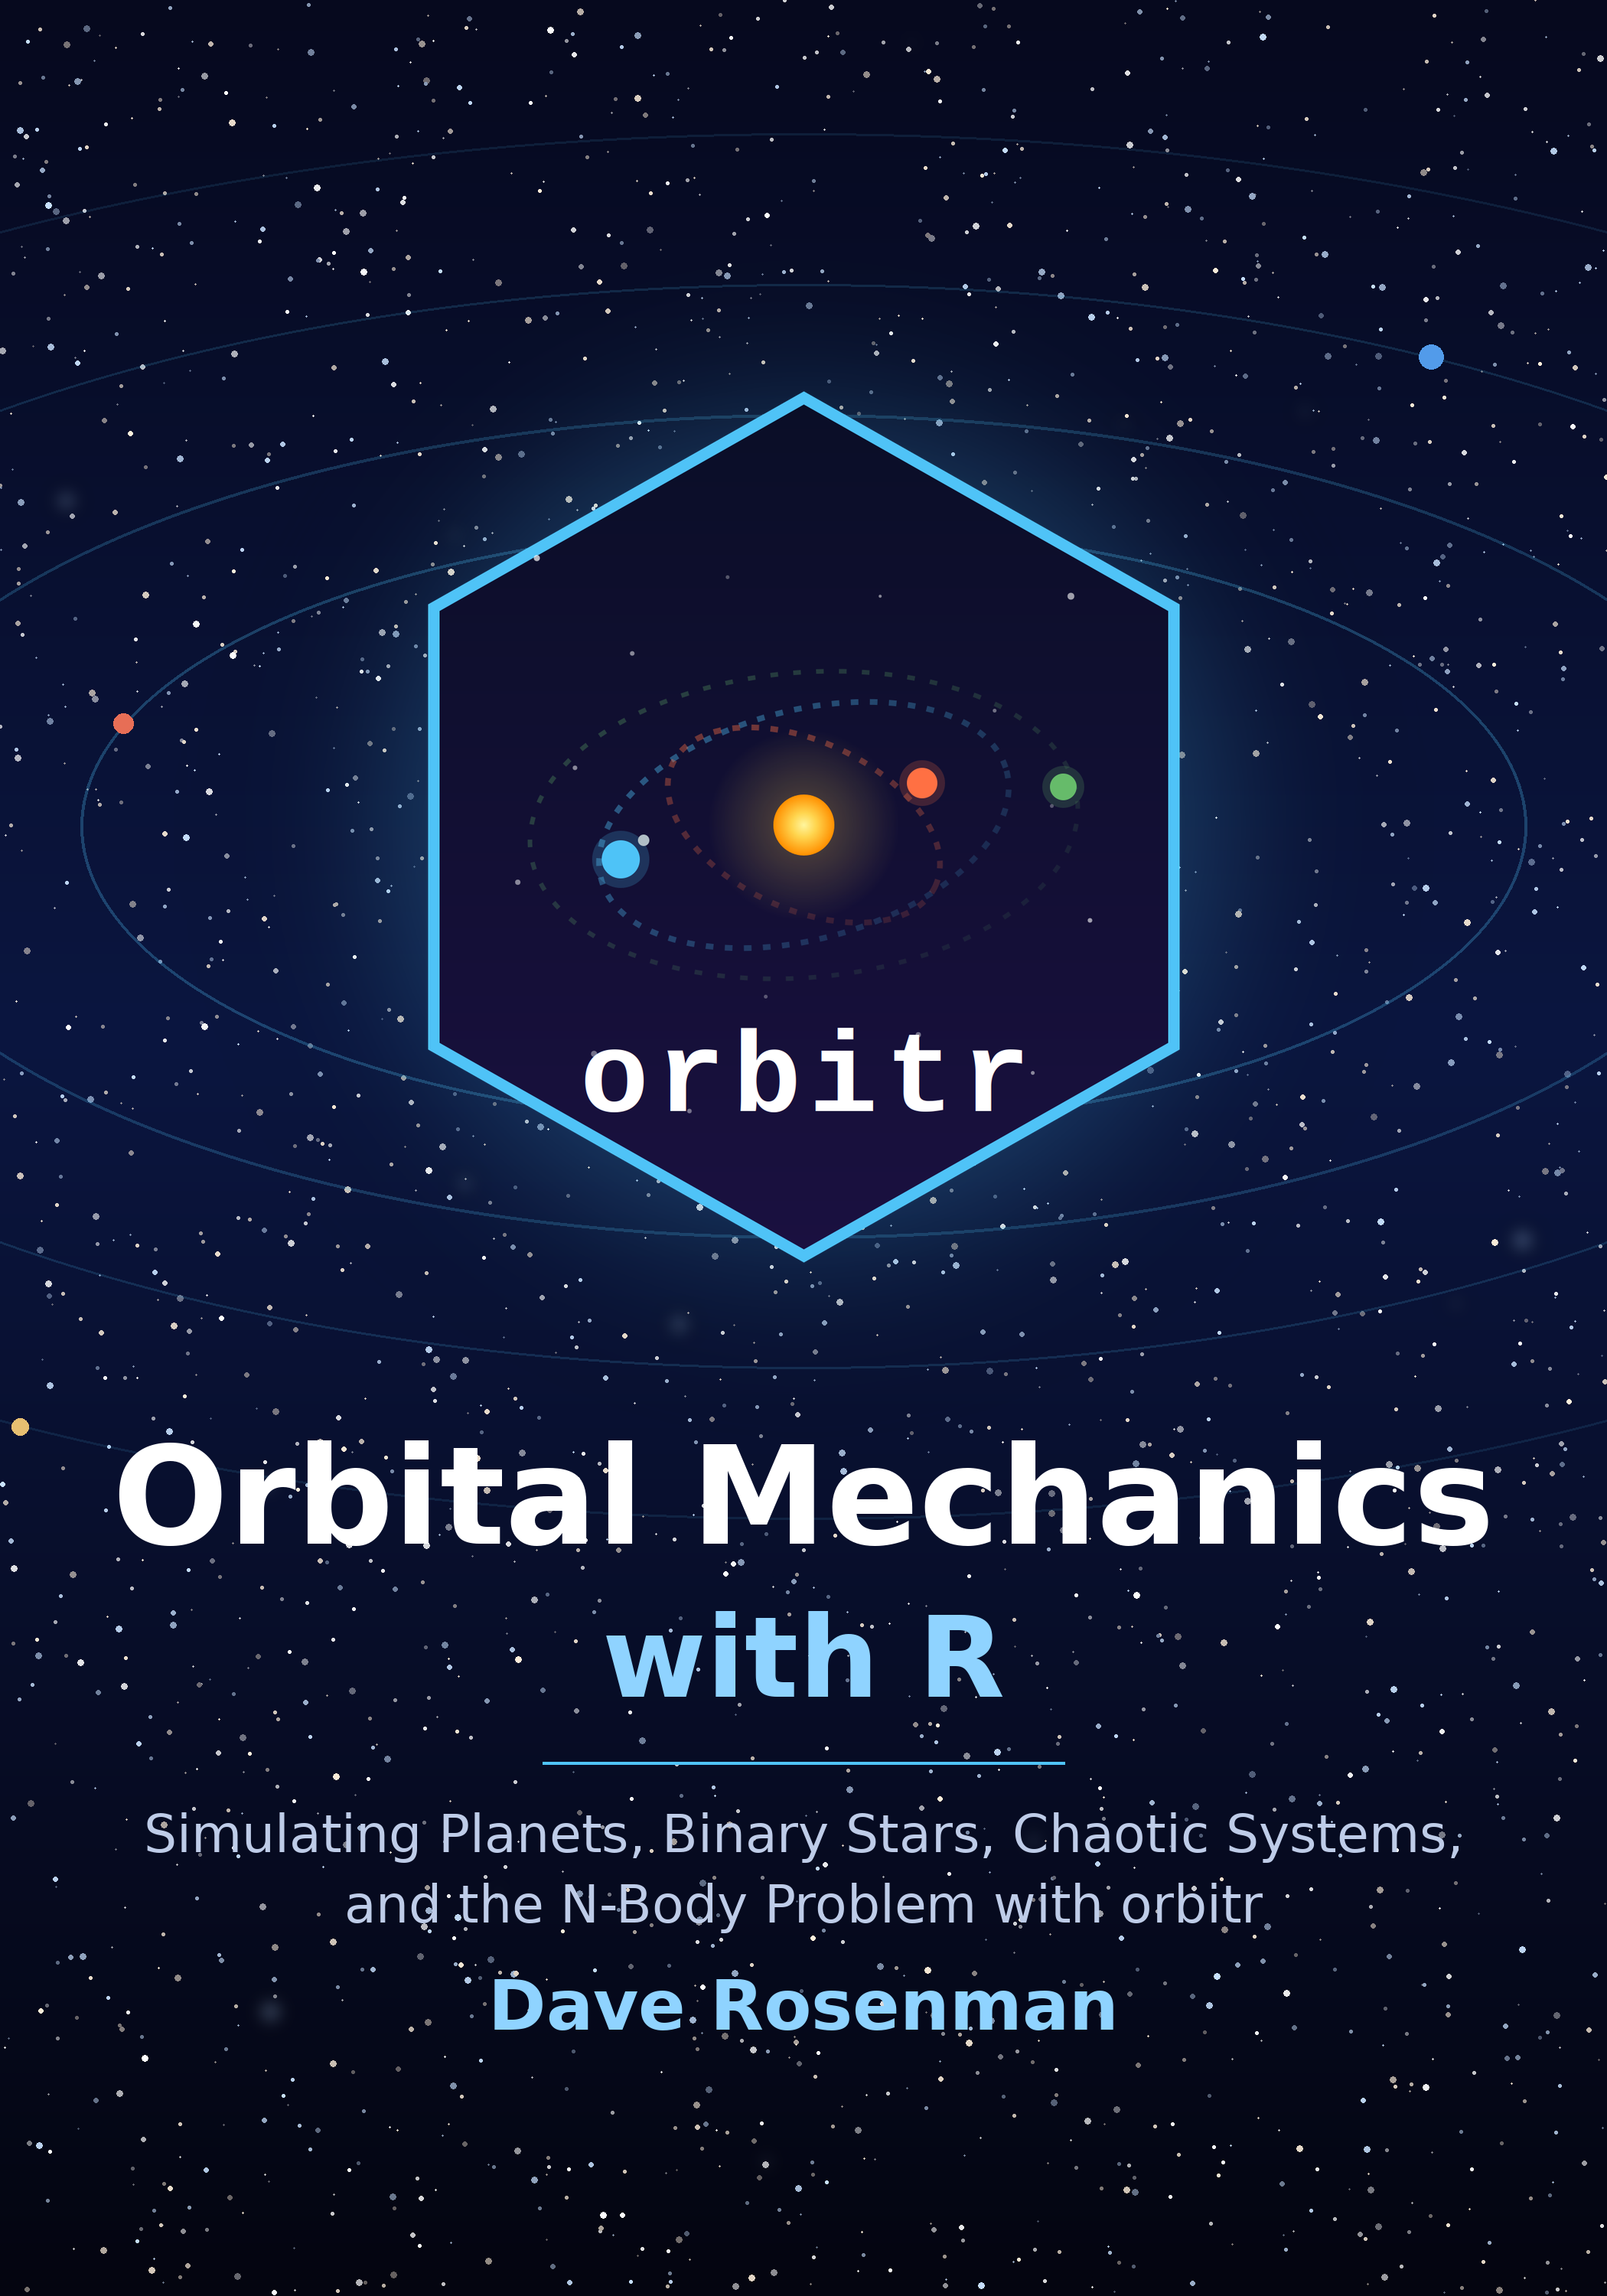
\includegraphics[width=\paperwidth,height=\paperheight]{cover-print.png}%
    \restoregeometry
  \end{titlepage}%
  \cleardoublepage
}

% Copyright page on the back of the title page (KOMA-Script prints
% \lowertitleback on the verso of the title page automatically).
\lowertitleback{%
  \small
  Copyright \textcopyright{} 2026 David P.~Rosenman\\[0.5ex]
  All rights reserved. No part of this book may be reproduced in any form
  without written permission from the author, except for brief quotations
  in reviews.\\[1.5ex]
  The orbitr package is free software released under the MIT License;
  see \url{https://orbit-r.com}. All code listings in this book may be
  used freely.\\[1.5ex]
  Written for orbitr version 1.0.0.\\[0.5ex]
  First edition.\\[1.5ex]
  % ISBN assigned by KDP:
  % ISBN 978-0-0000000-0-0
}
\makeatletter
\@ifpackageloaded{tcolorbox}{}{\usepackage[skins,breakable]{tcolorbox}}
\@ifpackageloaded{fontawesome5}{}{\usepackage{fontawesome5}}
\definecolor{quarto-callout-color}{HTML}{909090}
\definecolor{quarto-callout-note-color}{HTML}{0758E5}
\definecolor{quarto-callout-important-color}{HTML}{CC1914}
\definecolor{quarto-callout-warning-color}{HTML}{EB9113}
\definecolor{quarto-callout-tip-color}{HTML}{00A047}
\definecolor{quarto-callout-caution-color}{HTML}{FC5300}
\definecolor{quarto-callout-color-frame}{HTML}{acacac}
\definecolor{quarto-callout-note-color-frame}{HTML}{4582ec}
\definecolor{quarto-callout-important-color-frame}{HTML}{d9534f}
\definecolor{quarto-callout-warning-color-frame}{HTML}{f0ad4e}
\definecolor{quarto-callout-tip-color-frame}{HTML}{02b875}
\definecolor{quarto-callout-caution-color-frame}{HTML}{fd7e14}
\makeatother
\makeatletter
\@ifpackageloaded{bookmark}{}{\usepackage{bookmark}}
\makeatother
\makeatletter
\@ifpackageloaded{caption}{}{\usepackage{caption}}
\AtBeginDocument{%
\ifdefined\contentsname
  \renewcommand*\contentsname{Table of contents}
\else
  \newcommand\contentsname{Table of contents}
\fi
\ifdefined\listfigurename
  \renewcommand*\listfigurename{List of Figures}
\else
  \newcommand\listfigurename{List of Figures}
\fi
\ifdefined\listtablename
  \renewcommand*\listtablename{List of Tables}
\else
  \newcommand\listtablename{List of Tables}
\fi
\ifdefined\figurename
  \renewcommand*\figurename{Figure}
\else
  \newcommand\figurename{Figure}
\fi
\ifdefined\tablename
  \renewcommand*\tablename{Table}
\else
  \newcommand\tablename{Table}
\fi
}
\@ifpackageloaded{float}{}{\usepackage{float}}
\floatstyle{ruled}
\@ifundefined{c@chapter}{\newfloat{codelisting}{h}{lop}}{\newfloat{codelisting}{h}{lop}[chapter]}
\floatname{codelisting}{Listing}
\newcommand*\listoflistings{\listof{codelisting}{List of Listings}}
\usepackage{amsthm}
\theoremstyle{plain}
\newtheorem{theorem}{Theorem}[chapter]
\theoremstyle{remark}
\AtBeginDocument{\renewcommand*{\proofname}{Proof}}
\newtheorem*{remark}{Remark}
\newtheorem*{solution}{Solution}
\newtheorem{refremark}{Remark}[chapter]
\newtheorem{refsolution}{Solution}[chapter]
\makeatother
\makeatletter
\makeatother
\makeatletter
\@ifpackageloaded{caption}{}{\usepackage{caption}}
\@ifpackageloaded{subcaption}{}{\usepackage{subcaption}}
\makeatother
\usepackage{bookmark}
\IfFileExists{xurl.sty}{\usepackage{xurl}}{} % add URL line breaks if available
\urlstyle{same}
% fallback for those not using the hyperref driver hyperxmp:
\makeatletter
\@ifundefined{xmpquote}{\newcommand{\xmpquote}[1]{#1}}{}
\makeatother
\hypersetup{
  pdftitle={Orbital Mechanics with R},
  pdfauthor={Dave Rosenman},
  hidelinks,
  pdfcreator={LaTeX via pandoc}}


\title{Orbital Mechanics with R}
\usepackage{etoolbox}
\makeatletter
\providecommand{\subtitle}[1]{% add subtitle to \maketitle
  \apptocmd{\@title}{\par {\large #1 \par}}{}{}
}
\makeatother
\subtitle{Simulating Planets, Binary Stars, Chaotic Systems, and the
N-Body Problem with orbitr}
\author{Dave Rosenman}
\date{}
\begin{document}
\frontmatter
\maketitle

\renewcommand*\contentsname{Table of contents}
{
\setcounter{tocdepth}{1}
\tableofcontents
}

\mainmatter
\bookmarksetup{startatroot}

\chapter*{Preface}\label{preface}
\addcontentsline{toc}{chapter}{Preface}

\markboth{Preface}{Preface}

The documentation for orbitr lives at \url{https://orbit-r.com}, and it
is free. It will show you how to put a planet around a star in four
lines of R, how to load the whole solar system from real JPL data, and
how to animate a planet orbiting two suns. If all you want is to drive
the package, you may not need this book.

This book is about everything the documentation leaves out. The
documentation says that \texttt{simulate\_system()} uses the Velocity
Verlet method by default because it ``conserves energy over long
timescales.'' It does not say \emph{why} Verlet conserves energy when
the textbook Euler method does not, or where the method came from (a
1907 paper about the aurora, as it turns out), or how you would check
for yourself that it is doing its job. The documentation gives you the
circular-orbit speed \(v_{\mathrm{circ}} = \sqrt{GM/r}\) as a fact. It
does not derive it, and it does not tell you how that one formula,
pushed a little further, gives you Kepler's three laws, the shape of
every orbit in the solar system, and the velocity formulas that make the
Kepler-16 example work.

So this is two books in one. The first is a physics book that uses
orbitr the way a lab course uses a bench: every result gets derived on
paper and then checked against a simulation you can run yourself. The
second is an applications book that uses the physics to do real
astrophysics: verifying Kepler's third law across the solar system,
building a binary star from conservation of momentum, watching Mars go
retrograde from a geocentric frame, measuring how fast a chaotic triple
system forgets its initial conditions.

\section*{Who this book is for}\label{who-this-book-is-for}
\addcontentsline{toc}{section}{Who this book is for}

\markright{Who this book is for}

Two kinds of readers.

If you know R and are curious about how orbits work, this book will
teach you the physics using tools you already have. You will need
calculus and vectors, and it helps to have met Newton's laws once, but
you do not need to have taken a mechanics course. Where a derivation
needs a fact from mechanics, the fact is stated and explained.

If you are a physics or astronomy student and want to \emph{compute},
this book will show you how to turn the equations in your mechanics
course into working simulations, and how to use tidy data tools to
analyze what comes out. You do not need to know R at all.
Appendix~\ref{sec-r-basics} gets you from nothing to running the book's
code (installing R, packages, the pipe, the handful of dplyr and ggplot2
functions the book uses) in an hour, and points to the free books to
read when you want more. Every piece of code in the chapters is
explained, and the whole book uses a small, consistent vocabulary.

If the mathematics is the uncertain part, Appendix~\ref{sec-math}
collects everything the derivations assume (vectors and their products,
derivatives of vectors, polar coordinates, Taylor series, the geometry
of an ellipse) in one place, with the specific identities the book uses.

If you are both, you will find the two halves of the book talk to each
other more than you might expect. The best way to understand a
symplectic integrator is to watch a non-symplectic one fail; the best
way to understand an orbital element is to vary it and look.

\section*{What is in this book}\label{what-is-in-this-book}
\addcontentsline{toc}{section}{What is in this book}

\markright{What is in this book}

\textbf{Part I, First Orbits}, gets you running. Chapter 1 explains what
an N-body simulation is and why anyone bothers when Kepler already
solved the two-body problem. Chapter 2 walks through the four-line
pipeline and the tidy table it produces.

\textbf{Part II, Where the Physics Comes From}, is the heart of the
book. Chapter 3 starts from Newton's law and builds the N-body equations
of motion that the package integrates. Chapter 4 solves the two-body
problem by hand and derives everything the documentation states as fact:
the orbit equation, Kepler's laws, the vis-viva equation, circular and
escape velocity. Chapter 5 derives the three integrators (Euler,
Euler-Cromer, Velocity Verlet), shows why only two of them are fit for
orbits, and traces the Verlet method back through molecular dynamics,
the aurora, and the \emph{Principia}. Chapter 6 explains gravitational
softening. Chapter 7 derives the conversion from Keplerian orbital
elements to the Cartesian state vectors the engine actually uses.

\textbf{Part III, Doing Astrophysics with orbitr}, is the applications
half. Each chapter takes a problem from astronomy, sets it up from the
physics in Part II, runs it, and analyzes the result with dplyr and
ggplot2.

\textbf{Part IV, Under the Hood}, looks at the C++ engine and at the
places where a point-mass Newtonian model stops being enough.

The appendices collect the mathematical background the derivations
assume, the R needed to run the book, a quick function reference, and
the built-in physical constants with their sources.

\section*{What you need}\label{what-you-need}
\addcontentsline{toc}{section}{What you need}

\markright{What you need}

\begin{itemize}
\tightlist
\item
  R, version 4.1 or later, from \url{https://cran.r-project.org}. The
  book uses R's native pipe \texttt{\textbar{}\textgreater{}}
  everywhere.
\item
  The orbitr package, version 1.0.0 or later, from CRAN (see the box
  below).
\item
  The dplyr and ggplot2 packages. They are installed automatically with
  orbitr. A few chapters also use tidyr.
\item
  For the interactive 3D plots and the animations, the plotly,
  gganimate, and gifski packages. These are optional; the book tells you
  when it uses them.
\end{itemize}

An editor that runs R code chunks (RStudio or Positron, from
\url{https://posit.co}) makes it easy to run the book's examples as you
read.

\begin{tcolorbox}[enhanced jigsaw, arc=.35mm, bottomrule=.15mm, bottomtitle=1mm, breakable, colback=white, colbacktitle=quarto-callout-note-color!10!white, colframe=quarto-callout-note-color-frame, coltitle=black, left=2mm, leftrule=.75mm, opacityback=0, opacitybacktitle=0.6, rightrule=.15mm, title={Installing orbitr}, titlerule=0mm, toprule=.15mm, toptitle=1mm]

This book needs orbitr 1.0.0 or later, which is on CRAN:

\begin{Shaded}
\begin{Highlighting}[]
\FunctionTok{install.packages}\NormalTok{(}\StringTok{"orbitr"}\NormalTok{)}
\end{Highlighting}
\end{Shaded}

\texttt{packageVersion("orbitr")} should then report 1.0.0 or higher.
The development version, with whatever has been added since, is at
\url{https://github.com/DRosenman/orbitr} and installs with
\texttt{remotes::install\_github("DRosenman/orbitr")}; it compiles the
package's C++ engine, so on Windows that needs Rtools and on a Mac the
Xcode command-line tools. For this book, the CRAN version is the one to
use.

\end{tcolorbox}

The optional packages, in one line:

\begin{Shaded}
\begin{Highlighting}[]
\FunctionTok{install.packages}\NormalTok{(}\FunctionTok{c}\NormalTok{(}\StringTok{"tidyr"}\NormalTok{, }\StringTok{"plotly"}\NormalTok{, }\StringTok{"gganimate"}\NormalTok{, }\StringTok{"gifski"}\NormalTok{))}
\end{Highlighting}
\end{Shaded}

\section*{A note on versions}\label{a-note-on-versions}
\addcontentsline{toc}{section}{A note on versions}

\markright{A note on versions}

This book is written for orbitr 1.0.0, and every figure in it was
produced by that version. Version 1.0 is the point at which the
package's function names, arguments, and defaults became stable:
anything that changes afterwards will be deprecated first, so code in
this book should keep running on later versions, possibly with a warning
pointing at the replacement. Several of the analysis functions the book
uses (\texttt{get\_orbital\_elements()}, \texttt{get\_energy()},
\texttt{conserved\_quantities()}, \texttt{continue\_simulation()}, the
barycentric reference frame) were added in 1.0.0 because this book
needed them, so it will not run on 0.3.0. The physics in Part II does
not depend on the version at all.

\section*{How the code works}\label{how-the-code-works}
\addcontentsline{toc}{section}{How the code works}

\markright{How the code works}

Every figure and every number in this book was produced by the code
shown next to it, when the book was built. Nothing was pasted in from
elsewhere. That means two things for you as a reader. First, if you run
the code, you should get the same picture. Second, when the text says a
simulated period is ``about 27 days,'' that number came out of the
simulation, not out of my head.

Code appears in blocks like this, with output marked by
\texttt{\#\textgreater{}}:

\begin{Shaded}
\begin{Highlighting}[]
\FunctionTok{sqrt}\NormalTok{(gravitational\_constant }\SpecialCharTok{*}\NormalTok{ mass\_earth }\SpecialCharTok{/}\NormalTok{ distance\_earth\_moon)}
\CommentTok{\#\textgreater{} [1] 1018.289}
\end{Highlighting}
\end{Shaded}

Two kinds of output from orbitr do not survive the trip to paper.
Interactive 3D plots (\texttt{plot\_orbits\_3d()}, and
\texttt{plot\_orbits()} whenever a body moves in \(z\)) are plotly
widgets, and animations (\texttt{animate\_system()}) are GIFs.
Throughout the book I use static ggplot2 figures, which are the same in
every edition, and pass \texttt{three\_d\ =\ FALSE} wherever a system
has three-dimensional motion so that the figure stays flat.

Where the text discusses an animation or an interactive plot, the
printed book shows the call you would make and a static snapshot from
\texttt{plot\_system()} in place of the result. The online edition at
\url{https://book.orbit-r.com} shows them live.

\section*{Conventions}\label{conventions}
\addcontentsline{toc}{section}{Conventions}

\markright{Conventions}

All quantities are in SI units: meters, kilograms, seconds. The built-in
constants (\texttt{mass\_earth}, \texttt{distance\_earth\_sun},
\texttt{speed\_moon}, \ldots) are all SI, and all of the package's
arguments expect SI. Vectors are set in bold, \(\mathbf{r}\), and their
magnitudes in italic, \(r = |\mathbf{r}|\). Unit vectors wear a hat,
\(\hat{\mathbf{r}} = \mathbf{r}/r\). Dots denote time derivatives:
\(\dot{\mathbf{r}}\) is velocity and \(\ddot{\mathbf{r}}\) is
acceleration.

The symbol \(\mu\) always means the gravitational parameter
\(\mu = G(M + m)\) of a pair of bodies (or \(GM\) when one is much
heavier). Some mechanics texts use \(\mu\) for the reduced mass; this
book writes the reduced mass as \(m_r\) to avoid the clash.

A few helper functions that the text defines for the derivations
(measuring a period from a time series, solving Kepler's equation,
converting elements to a state vector by hand) are collected in the file
\texttt{R/helpers.R} in the book's source, which every chapter loads, so
later chapters use them without repeating the definitions. Everything
else is a package function.

Boxes marked \textbf{Where it comes from} give the history of a method
or a formula: who found it, what problem they were working on, and how
it ended up in the package. Boxes marked \textbf{Key result} collect the
formulas you will reuse.

\section*{Try it first: the orbitr
app}\label{try-it-first-the-orbitr-app}
\addcontentsline{toc}{section}{Try it first: the orbitr app}

\markright{Try it first: the orbitr app}

Before any code, it helps to have \emph{seen} an orbit respond to a
change: a planet given a little more speed and swinging out into an
ellipse, a time step pushed too far and the orbit falling apart. The
orbitr app is the package with a control panel on it. It runs in a
browser, needs no installation, and does nothing the code in this book
cannot do, which is the point: every control in it corresponds to an
argument of a function you will meet in Chapter 2, and when you later
type
\texttt{add\_body("Moon",\ mass\ =\ mass\_moon,\ x\ =\ distance\_earth\_moon,\ vy\ =\ speed\_moon)}
you will already know what happens when that \texttt{vy} goes up. The
app's \textbf{Code} tab makes that correspondence explicit: whatever
system you have set up, it shows the R code that produces exactly what
is on the screen. Set up a system by clicking, read the code, paste it
into R, and you have run your first simulation.

The app is at \url{https://daverosenman.shinyapps.io/orbitr/}, or scan
the code below. The online edition of this book at
\url{https://book.orbit-r.com} embeds it in this page, with a guided
walkthrough of what to try.

\begin{center}

\includegraphics[width=0.38\linewidth,height=\textheight,keepaspectratio]{qr-app.png}
\end{center}

Ten minutes with it is a good investment before Chapter 2. Suggested
experiments, in order: pick a preset system and run it as is; change one
body's starting speed by ten percent in each direction and run again;
shorten and lengthen the time step until something looks wrong; switch
the integrator from Verlet to Euler and run the same system. After each
one, open the Code tab and see which argument changed. Chapters 4 and 5
explain what you just saw.

\section*{Acknowledgments}\label{acknowledgments}
\addcontentsline{toc}{section}{Acknowledgments}

\markright{Acknowledgments}

The physics in this book was shaped by Thornton and Marion's
\emph{Classical Dynamics} (Thornton and Marion 2004) and Newman's
\emph{Computational Physics} (Newman 2012), the two books I kept open
while writing the engine. The N-body methods follow Aarseth (Aarseth
2003).

\section*{Dedication}\label{dedication}
\addcontentsline{toc}{section}{Dedication}

\markright{Dedication}

For Kerry, a true academic, with a mind so beautiful it is hard to
believe it runs on the laws of physics.

For my parents, who supported me through not one undergraduate degree
but two: political science at Temple, and then, when I announced the
crazy idea of studying theoretical physics, that one as well.

And for my grandfather, a math teacher, for a million things, among them
the algebra and trigonometry he taught me all over again before I could
start on physics; and for my grandmother, who powered every one of those
sessions with the best Italian food on the planet.

\part{First Orbits}

\chapter{Why Simulate Gravity?}\label{sec-why-simulate}

In 1609 Johannes Kepler published the first two of his three laws of
planetary motion, and in 1687 Isaac Newton showed that all three follow
from a single inverse-square force law (Kepler 1609; Newton 1687). For
one planet going around one star, the problem is \emph{solved}: write
down the initial position and velocity, and the orbit is an ellipse
whose size, shape, and orientation you can compute by hand, exactly, for
all time. Chapter 4 does exactly that.

So why would anyone simulate it?

\section{Three reasons}\label{three-reasons}

\textbf{Because two is a special number.} Add a third body and the exact
solution disappears. Newton knew it; he spent years on the Moon's motion
under the combined pull of the Earth and the Sun and reportedly said it
was the only problem that ever made his head ache. In 1890 Henri
Poincaré proved that the three-body problem has no general solution of
the kind Kepler's ellipses provide, and in doing so discovered what we
now call chaos (Poincaré 1890). Our own solar system has one star, eight
planets, hundreds of moons, and a great many smaller things, every one
of which pulls on every other. The planets follow Kepler's ellipses
\emph{almost}, and the ``almost'' contains all of the interesting
physics: Jupiter tugging Earth's orbit, resonances in the asteroid belt,
the slow precession of Mercury's perihelion. None of it can be written
down in closed form. All of it can be simulated.

\textbf{Because the solution and the understanding are different
things.} Even for the two-body problem, knowing that the answer is an
ellipse is not the same as knowing what happens when you give a planet
20\% too much speed, or launch it at the wrong angle, or put it around a
star of twice the mass. A simulation lets you ask those questions in
seconds and \emph{see} the answer. Most of the intuition that working
astronomers have about orbits was built this way, by changing something
and looking.

\textbf{Because the simulation is the check on the theory.} When you
derive, on paper, that a body launched at \(\sqrt{2}\) times the
circular speed should just barely escape, you can set up that exact
situation and watch. If the simulation agrees, you understand both the
physics and the code a little better. If it disagrees, one of them is
wrong, and finding out which is where the learning is. Part II of this
book is built around that loop: derive, simulate, compare.

\section{What a simulation actually
is}\label{what-a-simulation-actually-is}

Here is the whole idea in four sentences. At any instant, every body has
a position and a velocity. Newton's law tells you the acceleration of
every body from the positions of all the others. If you know where
things are and how fast they are moving right now, you can estimate
where they will be a short time \(\Delta t\) later. Do that, then do it
again from the new state, and again, and you have an orbit.

The ``estimate'' is the whole subject of numerical integration, and it
is where the craft is. The computer never solves the equations of
motion. It takes small steps and hopes the error in each step is small
enough, and cancels well enough, that the result after a million steps
still means something. Whether that hope is justified depends entirely
on \emph{how} you take the step. Chapter 5 derives three ways of doing
it, and shows that the most obvious one, the one every introductory text
starts with, produces orbits that spiral outward and planets that
quietly gain energy from nowhere. The one the package uses by default
was invented for a different problem entirely and has a surprisingly
deep reason for working.

This discreteness is the one thing to keep in mind every time you look
at a simulation result. A simulated orbit is not the true orbit; it is
the true orbit plus an error that depends on the step size and the
method. Most of the time the error is invisible. Part of learning to
simulate is learning when it is not.

\section{What orbitr is}\label{what-orbitr-is}

orbitr is an N-body gravitational simulator written for R (Rosenman
2026). You build a system by adding bodies to it with masses, positions,
and velocities, run it forward in time, and get back a table. A few
things make it different from the N-body codes that research astronomers
use, and they are the reasons this book is possible:

\begin{itemize}
\tightlist
\item
  \textbf{The output is a tibble.} One row per body per time step, with
  columns for time, position, and velocity. There is no special result
  object to learn. Every tool in the R data-analysis ecosystem (dplyr,
  ggplot2, plotly, anything that takes a data frame) works on it
  directly. Most of the analysis in this book is a \texttt{filter()}, a
  \texttt{mutate()}, and a \texttt{ggplot()}.
\item
  \textbf{It is built for the pipe.} A simulation reads top to bottom:
  create a system, add bodies, simulate, plot.
\item
  \textbf{Analysis is built in.} The output can be re-centered on any
  body or on the system's center of mass, reduced to orbital elements,
  checked against the conservation laws, and continued from where it
  stopped, each with one function.
\item
  \textbf{The physics is visible.} Three integration methods are
  available, so you can compare them. Softening is optional and off by
  default, so you get exact Newtonian gravity unless you ask otherwise.
  The gravitational constant is an argument, so you can turn gravity up,
  down, or off.
\item
  \textbf{Real data is built in.} Masses, orbital distances, and speeds
  for the Sun, the planets, and the Moon are included as constants, and
  the planets' orbital elements come from the JPL DE440 ephemeris (Park
  et al. 2021), so \texttt{add\_planet("Mars",\ parent\ =\ "Sun")} puts
  Mars where Mars actually is.
\item
  \textbf{The inner loop is compiled.} The pairwise force calculation
  runs in C++ through Rcpp (Eddelbuettel and François 2011), with a
  pure-R fallback, so systems of a few dozen bodies simulate in seconds.
\end{itemize}

\section{What orbitr is not}\label{what-orbitr-is-not}

It is not an ephemeris. If you need to know where Mars will be on a
given date to arc-second precision, use JPL Horizons, which fits decades
of radar and spacecraft tracking data and includes effects this package
ignores. orbitr starts from JPL's orbital elements at one epoch and
integrates pure point-mass Newtonian gravity forward. Over a few years
the planets land close to where they should; over centuries, small
omitted effects accumulate.

The omissions are deliberate, and knowing them tells you what the
package can and cannot answer:

\begin{itemize}
\tightlist
\item
  Bodies are point masses. Gravity outside a spherically symmetric body
  is exactly that of a point mass at its center (Chapter 3 proves this),
  so for orbital distances this costs nothing. But there is no notion of
  two bodies touching, no oblateness, no tides.
\item
  Gravity is Newtonian. General relativity's correction to Mercury's
  perihelion precession, 43 arcseconds per century, is not in the model.
\item
  There are no non-gravitational forces: no atmospheric drag, no
  radiation pressure, no thrust.
\item
  The time step is fixed. Orbits that pass very close to a massive body
  need small steps near periapsis and would happily take large ones
  elsewhere; orbitr takes the same step throughout. Chapter 13 shows
  where this bites and how to handle it.
\end{itemize}

Chapter 16 returns to each of these, and to the package roadmap.

\section{How to read this book}\label{how-to-read-this-book}

If you want to get something running first, go to Chapter 2 now, then
come back. Part II can be read straight through as a physics text; the
code is there to check the physics, not the other way round. Part III
assumes Part II but each chapter stands alone, so you can go straight to
binary stars or chaos if that is what you came for.

The most useful habit while reading is to predict before you run. Each
chapter's code sets up something whose outcome the physics tells you in
advance; say what you expect, then look. When the two disagree, one of
them is wrong, and finding out which is where the learning is.

\section{Setting up}\label{setting-up}

The preface lists what to install and how; the short version is R,
orbitr 1.0.0 or later, and an editor that runs code chunks. Once that is
done, compare your versions with the ones this book was built with:

\begin{Shaded}
\begin{Highlighting}[]
\FunctionTok{packageVersion}\NormalTok{(}\StringTok{"orbitr"}\NormalTok{)}
\CommentTok{\#\textgreater{} [1] \textquotesingle{}1.0.0\textquotesingle{}}
\NormalTok{R.version.string}
\CommentTok{\#\textgreater{} [1] "R version 4.6.1 (2026{-}06{-}24 ucrt)"}
\end{Highlighting}
\end{Shaded}

If \texttt{packageVersion("orbitr")} reports something older than 1.0.0,
update: the analysis functions this book relies on were added in 1.0.0.
Anything newer should run the book's code unchanged; the changelog
(\texttt{NEWS.md} in the GitHub repository,
\url{https://github.com/DRosenman/orbitr}) lists any deprecations.

\chapter{Four Lines to an Orbit}\label{sec-four-lines}

This chapter gets you from nothing to a working simulation, then slows
down and looks carefully at each piece. By the end you will know what
every argument in the four-line pipeline does, what the table it
produces looks like, and one subtle thing the four-line version gets
slightly wrong, which turns out to be a preview of a real conservation
law.

\section{The Moon in four lines}\label{the-moon-in-four-lines}

\begin{Shaded}
\begin{Highlighting}[]
\FunctionTok{library}\NormalTok{(orbitr)}

\FunctionTok{create\_system}\NormalTok{() }\SpecialCharTok{|\textgreater{}}
  \FunctionTok{add\_body}\NormalTok{(}\StringTok{"Earth"}\NormalTok{, }\AttributeTok{mass =}\NormalTok{ mass\_earth) }\SpecialCharTok{|\textgreater{}}
  \FunctionTok{add\_body}\NormalTok{(}\StringTok{"Moon"}\NormalTok{, }\AttributeTok{mass =}\NormalTok{ mass\_moon, }\AttributeTok{x =}\NormalTok{ distance\_earth\_moon, }\AttributeTok{vy =}\NormalTok{ speed\_moon) }\SpecialCharTok{|\textgreater{}}
  \FunctionTok{simulate\_system}\NormalTok{(}\AttributeTok{time\_step =}\NormalTok{ seconds\_per\_hour, }\AttributeTok{duration =}\NormalTok{ seconds\_per\_day }\SpecialCharTok{*} \DecValTok{28}\NormalTok{) }\SpecialCharTok{|\textgreater{}}
  \FunctionTok{plot\_orbits}\NormalTok{()}
\end{Highlighting}
\end{Shaded}

\begin{figure}[tbp]

\centering{

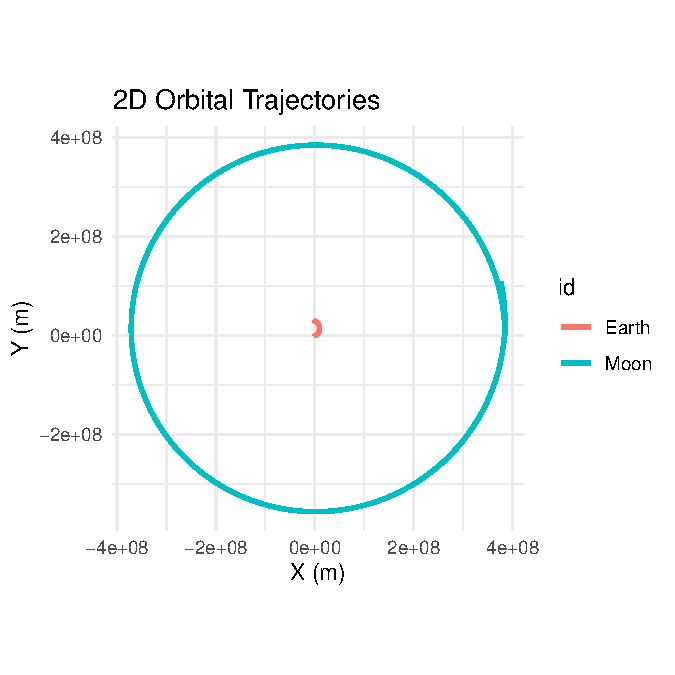
\includegraphics[width=0.7\linewidth,height=\textheight,keepaspectratio]{02-four-lines-to-an-orbit_files/figure-pdf/fig-moon-four-lines-1.pdf}

}

\caption{\label{fig-moon-four-lines}The Moon's orbit around Earth over
28 days, simulated one hour at a time.}

\end{figure}%

Earth sits at the origin. The Moon starts 384,400 km away along the
\(x\) axis, moving at 1,022 m/s in the \(+y\) direction, and 28 days
later it has gone around once. (The Earth's own path is in there too; it
is too small to see at this scale. We will come back to it.)

\section{What each line does}\label{what-each-line-does}

\textbf{\texttt{create\_system()}} makes an empty system. Its one
argument is the gravitational constant, \texttt{G}, which defaults to
the real value, \(6.6743\times10^{-11}\ \mathrm{m^3\,kg^{-1}\,s^{-2}}\).
You will almost never change it, but it is there, and setting it to zero
is a quick way to confirm that a body with no forces on it moves in a
straight line.

\textbf{\texttt{add\_body()}} adds one body. It needs a name
(\texttt{id}) and a \texttt{mass}; everything else defaults to zero. The
position arguments \texttt{x}, \texttt{y}, \texttt{z} are in meters and
the velocity arguments \texttt{vx}, \texttt{vy}, \texttt{vz} in meters
per second. Earth gets only a mass, so it starts at the origin at rest.
The Moon gets a mass, an \(x\) position, and a \(y\) velocity. The
constants \texttt{mass\_earth}, \texttt{mass\_moon},
\texttt{distance\_earth\_moon}, and \texttt{speed\_moon} are exported by
the package; Appendix~\ref{sec-constants} lists all of them with their
sources.

\textbf{\texttt{simulate\_system()}} runs the integration.
\texttt{time\_step} is the size of each step in seconds and
\texttt{duration} is how long to run, also in seconds. Here that is one
hour per step for 28 days, or \(28\times24 = 672\) steps. The defaults
are one hour and one year. Two more arguments matter and have sensible
defaults: \texttt{method}, which picks the integrator (\texttt{"verlet"}
by default; Chapter 5), and \texttt{softening}, which is zero by
default, meaning exact Newtonian gravity (Chapter 6).

\textbf{\texttt{plot\_orbits()}} draws the path of every body with
ggplot2 and returns the plot. Because it is an ordinary ggplot object
you can add layers to it with \texttt{+}.

The constants \texttt{seconds\_per\_hour}, \texttt{seconds\_per\_day},
and \texttt{seconds\_per\_year} exist because every time argument in the
package is in seconds, and nobody wants to type 2419200.

\section{What came back}\label{what-came-back}

Drop the plotting step and keep the result:

\begin{Shaded}
\begin{Highlighting}[]
\NormalTok{moon }\OtherTok{\textless{}{-}} \FunctionTok{create\_system}\NormalTok{() }\SpecialCharTok{|\textgreater{}}
  \FunctionTok{add\_body}\NormalTok{(}\StringTok{"Earth"}\NormalTok{, }\AttributeTok{mass =}\NormalTok{ mass\_earth) }\SpecialCharTok{|\textgreater{}}
  \FunctionTok{add\_body}\NormalTok{(}\StringTok{"Moon"}\NormalTok{, }\AttributeTok{mass =}\NormalTok{ mass\_moon, }\AttributeTok{x =}\NormalTok{ distance\_earth\_moon, }\AttributeTok{vy =}\NormalTok{ speed\_moon) }\SpecialCharTok{|\textgreater{}}
  \FunctionTok{simulate\_system}\NormalTok{(}\AttributeTok{time\_step =}\NormalTok{ seconds\_per\_hour, }\AttributeTok{duration =}\NormalTok{ seconds\_per\_day }\SpecialCharTok{*} \DecValTok{28}\NormalTok{)}

\NormalTok{moon}
\CommentTok{\#\textgreater{} \# A tibble: 1,346 x 9}
\CommentTok{\#\textgreater{}    id       mass          x           y     z      vx          vy    vz  time}
\CommentTok{\#\textgreater{}    \textless{}chr\textgreater{}   \textless{}dbl\textgreater{}      \textless{}dbl\textgreater{}       \textless{}dbl\textgreater{} \textless{}dbl\textgreater{}   \textless{}dbl\textgreater{}       \textless{}dbl\textgreater{} \textless{}dbl\textgreater{} \textless{}dbl\textgreater{}}
\CommentTok{\#\textgreater{}  1 Earth 5.97e24         0         0        0   0        0            0     0}
\CommentTok{\#\textgreater{}  2 Moon  7.34e22 384400000         0        0   0     1022            0     0}
\CommentTok{\#\textgreater{}  3 Earth 5.97e24       215.        0        0   0.119    0.000571     0  3600}
\CommentTok{\#\textgreater{}  4 Moon  7.34e22 384382520.  3679200        0  {-}9.71  1022.           0  3600}
\CommentTok{\#\textgreater{}  5 Earth 5.97e24       860.        4.11     0   0.239    0.00229      0  7200}
\CommentTok{\#\textgreater{}  6 Moon  7.34e22 384330083.  7358065.       0 {-}19.4   1022.           0  7200}
\CommentTok{\#\textgreater{}  7 Earth 5.97e24      1934.       16.5      0   0.358    0.00514      0 10800}
\CommentTok{\#\textgreater{}  8 Moon  7.34e22 384242692. 11036262.       0 {-}29.1   1022.           0 10800}
\CommentTok{\#\textgreater{}  9 Earth 5.97e24      3438.       41.1      0   0.477    0.00914      0 14400}
\CommentTok{\#\textgreater{} 10 Moon  7.34e22 384120357. 14713454.       0 {-}38.8   1021.           0 14400}
\CommentTok{\#\textgreater{} \# i 1,336 more rows}
\end{Highlighting}
\end{Shaded}

It is a tibble. Each row is one body at one instant. There are 1346
rows: two bodies, times 673 time steps, which is the 672 steps plus the
initial state. The columns are the body's \texttt{id}, its
\texttt{mass}, its position \texttt{x,\ y,\ z}, its velocity
\texttt{vx,\ vy,\ vz}, and \texttt{time} in seconds from the start.

That is the entire output format. There is nothing else to learn, which
is the point: everything you already know how to do with a data frame
works. How far is the Moon from the origin at the end of the run?

\begin{Shaded}
\begin{Highlighting}[]
\NormalTok{moon }\SpecialCharTok{|\textgreater{}}
  \FunctionTok{filter}\NormalTok{(time }\SpecialCharTok{==} \FunctionTok{max}\NormalTok{(time)) }\SpecialCharTok{|\textgreater{}}
  \FunctionTok{mutate}\NormalTok{(}\AttributeTok{r\_km =} \FunctionTok{sqrt}\NormalTok{(x}\SpecialCharTok{\^{}}\DecValTok{2} \SpecialCharTok{+}\NormalTok{ y}\SpecialCharTok{\^{}}\DecValTok{2} \SpecialCharTok{+}\NormalTok{ z}\SpecialCharTok{\^{}}\DecValTok{2}\NormalTok{) }\SpecialCharTok{/} \FloatTok{1e3}\NormalTok{) }\SpecialCharTok{|\textgreater{}}
  \FunctionTok{select}\NormalTok{(id, time, r\_km)}
\CommentTok{\#\textgreater{} \# A tibble: 2 x 3}
\CommentTok{\#\textgreater{}   id       time    r\_km}
\CommentTok{\#\textgreater{}   \textless{}chr\textgreater{}   \textless{}dbl\textgreater{}   \textless{}dbl\textgreater{}}
\CommentTok{\#\textgreater{} 1 Earth 2419200  29053.}
\CommentTok{\#\textgreater{} 2 Moon  2419200 391550.}
\end{Highlighting}
\end{Shaded}

How does the Moon's distance change over the month?

\begin{Shaded}
\begin{Highlighting}[]
\FunctionTok{library}\NormalTok{(dplyr)}
\FunctionTok{library}\NormalTok{(ggplot2)}

\NormalTok{moon }\SpecialCharTok{|\textgreater{}}
  \FunctionTok{filter}\NormalTok{(id }\SpecialCharTok{==} \StringTok{"Moon"}\NormalTok{) }\SpecialCharTok{|\textgreater{}}
  \FunctionTok{mutate}\NormalTok{(}\AttributeTok{r\_km =} \FunctionTok{sqrt}\NormalTok{(x}\SpecialCharTok{\^{}}\DecValTok{2} \SpecialCharTok{+}\NormalTok{ y}\SpecialCharTok{\^{}}\DecValTok{2} \SpecialCharTok{+}\NormalTok{ z}\SpecialCharTok{\^{}}\DecValTok{2}\NormalTok{) }\SpecialCharTok{/} \FloatTok{1e3}\NormalTok{) }\SpecialCharTok{|\textgreater{}}
  \FunctionTok{ggplot}\NormalTok{(}\FunctionTok{aes}\NormalTok{(time }\SpecialCharTok{/}\NormalTok{ seconds\_per\_day, r\_km)) }\SpecialCharTok{+}
  \FunctionTok{geom\_line}\NormalTok{() }\SpecialCharTok{+}
  \FunctionTok{labs}\NormalTok{(}\AttributeTok{x =} \StringTok{"Day"}\NormalTok{, }\AttributeTok{y =} \StringTok{"Distance from origin (km)"}\NormalTok{)}
\end{Highlighting}
\end{Shaded}

\begin{figure}[tbp]

\centering{

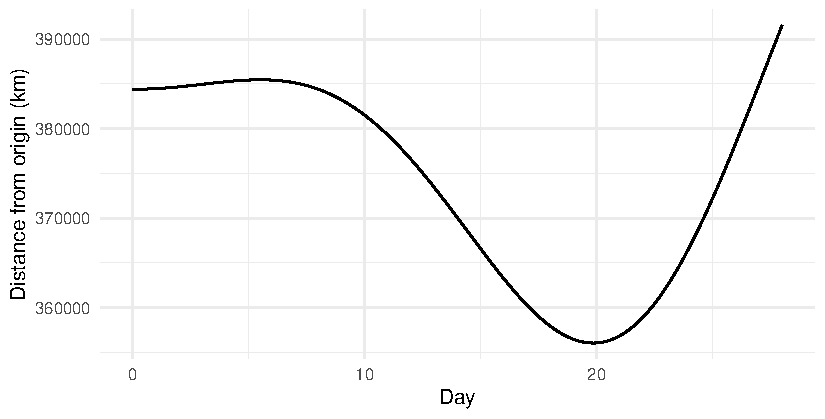
\includegraphics[width=1\linewidth,height=\textheight,keepaspectratio]{02-four-lines-to-an-orbit_files/figure-pdf/fig-moon-distance-1.pdf}

}

\caption{\label{fig-moon-distance}The Moon's distance from the origin
over the 28-day run. It is not quite constant: the orbit is slightly
elliptical.}

\end{figure}%

The distance dips and recovers: the orbit is an ellipse, not a circle,
because 1,022 m/s is not exactly the speed that produces a circle at
this distance. The speed that does is \(\sqrt{G(M+m)/r}\), which
evaluates to

\begin{Shaded}
\begin{Highlighting}[]
\FunctionTok{sqrt}\NormalTok{(gravitational\_constant }\SpecialCharTok{*}\NormalTok{ (mass\_earth }\SpecialCharTok{+}\NormalTok{ mass\_moon) }\SpecialCharTok{/}\NormalTok{ distance\_earth\_moon)}
\CommentTok{\#\textgreater{} [1] 1024.529}
\end{Highlighting}
\end{Shaded}

m/s. Chapter 4 derives that formula and shows how the small gap between
it and 1,022 m/s determines the eccentricity of the orbit in
Figure~\ref{fig-moon-distance}. For now, just notice that the simulation
knows about it without being told.

\section{Where did Earth go?}\label{where-did-earth-go}

I said Earth's path was too small to see. Let's look at it on its own:

\begin{Shaded}
\begin{Highlighting}[]
\NormalTok{moon }\SpecialCharTok{|\textgreater{}}
  \FunctionTok{filter}\NormalTok{(id }\SpecialCharTok{==} \StringTok{"Earth"}\NormalTok{) }\SpecialCharTok{|\textgreater{}}
  \FunctionTok{ggplot}\NormalTok{(}\FunctionTok{aes}\NormalTok{(x }\SpecialCharTok{/} \FloatTok{1e3}\NormalTok{, y }\SpecialCharTok{/} \FloatTok{1e3}\NormalTok{)) }\SpecialCharTok{+}
  \FunctionTok{geom\_path}\NormalTok{() }\SpecialCharTok{+}
  \FunctionTok{coord\_equal}\NormalTok{() }\SpecialCharTok{+}
  \FunctionTok{labs}\NormalTok{(}\AttributeTok{x =} \StringTok{"x (km)"}\NormalTok{, }\AttributeTok{y =} \StringTok{"y (km)"}\NormalTok{)}
\end{Highlighting}
\end{Shaded}

\begin{figure}[tbp]

\centering{

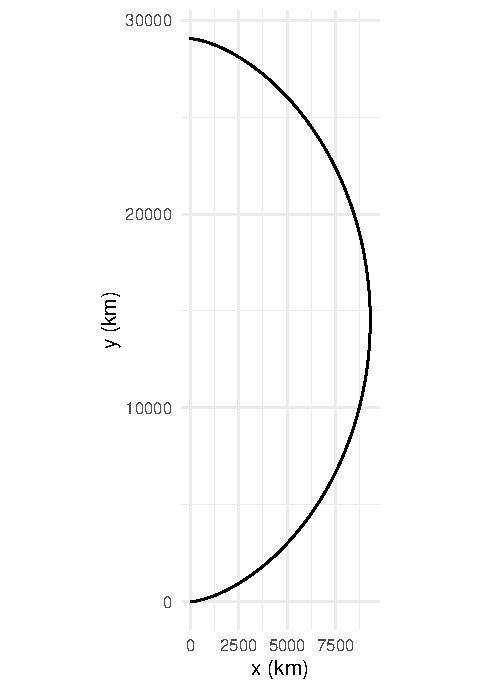
\includegraphics[width=0.45\linewidth,height=\textheight,keepaspectratio]{02-four-lines-to-an-orbit_files/figure-pdf/fig-earth-drift-1.pdf}

}

\caption{\label{fig-earth-drift}Earth's own motion during the 28-day
run. It loops once around the pair's center of mass while the whole
system drifts in the \(+y\) direction.}

\end{figure}%

Earth does not stay at the origin. It makes a small loop, as it should,
because the Moon pulls on Earth just as Earth pulls on the Moon, and the
two orbit their common center of mass. But the loop also \emph{drifts}:
after 28 days Earth has moved about

\begin{Shaded}
\begin{Highlighting}[]
\NormalTok{drift\_km }\OtherTok{\textless{}{-}}\NormalTok{ moon }\SpecialCharTok{|\textgreater{}}
  \FunctionTok{filter}\NormalTok{(id }\SpecialCharTok{==} \StringTok{"Earth"}\NormalTok{, time }\SpecialCharTok{==} \FunctionTok{max}\NormalTok{(time)) }\SpecialCharTok{|\textgreater{}}
  \FunctionTok{mutate}\NormalTok{(}\AttributeTok{r\_km =} \FunctionTok{sqrt}\NormalTok{(x}\SpecialCharTok{\^{}}\DecValTok{2} \SpecialCharTok{+}\NormalTok{ y}\SpecialCharTok{\^{}}\DecValTok{2}\NormalTok{) }\SpecialCharTok{/} \FloatTok{1e3}\NormalTok{) }\SpecialCharTok{|\textgreater{}}
  \FunctionTok{pull}\NormalTok{(r\_km)}
\FunctionTok{round}\NormalTok{(drift\_km)}
\CommentTok{\#\textgreater{} [1] 29053}
\end{Highlighting}
\end{Shaded}

kilometers from where it started. Nothing is wrong with the simulation.
The drift is the simulation being \emph{right} about something we got
wrong in the setup.

We gave the Moon momentum,
\(m_{\mathrm{Moon}} \times 1022\ \mathrm{m/s}\) in the \(+y\) direction,
and gave Earth none. The total momentum of the system is therefore not
zero, and since gravity is an internal force, total momentum is
conserved: the system's center of mass has to keep moving at a constant
velocity forever. That velocity is the Moon's momentum divided by the
total mass,

\begin{Shaded}
\begin{Highlighting}[]
\NormalTok{v\_com }\OtherTok{\textless{}{-}}\NormalTok{ mass\_moon }\SpecialCharTok{*}\NormalTok{ speed\_moon }\SpecialCharTok{/}\NormalTok{ (mass\_earth }\SpecialCharTok{+}\NormalTok{ mass\_moon)}
\NormalTok{v\_com}
\CommentTok{\#\textgreater{} [1] 12.41192}
\end{Highlighting}
\end{Shaded}

about 12 m/s, which over 28 days is \ensuremath{3.0027\times 10^{4}} km.
That is the drift in Figure~\ref{fig-earth-drift}, exactly.

The fix is to give Earth the equal and opposite momentum so the total is
zero. Earth's velocity must be
\(-v_{\mathrm{Moon}}\, m_{\mathrm{Moon}}/m_{\mathrm{Earth}}\):

\begin{Shaded}
\begin{Highlighting}[]
\NormalTok{v\_earth }\OtherTok{\textless{}{-}} \SpecialCharTok{{-}}\NormalTok{speed\_moon }\SpecialCharTok{*}\NormalTok{ mass\_moon }\SpecialCharTok{/}\NormalTok{ mass\_earth}

\NormalTok{moon\_fixed }\OtherTok{\textless{}{-}} \FunctionTok{create\_system}\NormalTok{() }\SpecialCharTok{|\textgreater{}}
  \FunctionTok{add\_body}\NormalTok{(}\StringTok{"Earth"}\NormalTok{, }\AttributeTok{mass =}\NormalTok{ mass\_earth, }\AttributeTok{vy =}\NormalTok{ v\_earth) }\SpecialCharTok{|\textgreater{}}
  \FunctionTok{add\_body}\NormalTok{(}\StringTok{"Moon"}\NormalTok{, }\AttributeTok{mass =}\NormalTok{ mass\_moon, }\AttributeTok{x =}\NormalTok{ distance\_earth\_moon, }\AttributeTok{vy =}\NormalTok{ speed\_moon) }\SpecialCharTok{|\textgreater{}}
  \FunctionTok{simulate\_system}\NormalTok{(}\AttributeTok{time\_step =}\NormalTok{ seconds\_per\_hour, }\AttributeTok{duration =}\NormalTok{ seconds\_per\_day }\SpecialCharTok{*} \DecValTok{28}\NormalTok{)}

\NormalTok{moon\_fixed }\SpecialCharTok{|\textgreater{}}
  \FunctionTok{filter}\NormalTok{(id }\SpecialCharTok{==} \StringTok{"Earth"}\NormalTok{) }\SpecialCharTok{|\textgreater{}}
  \FunctionTok{ggplot}\NormalTok{(}\FunctionTok{aes}\NormalTok{(x }\SpecialCharTok{/} \FloatTok{1e3}\NormalTok{, y }\SpecialCharTok{/} \FloatTok{1e3}\NormalTok{)) }\SpecialCharTok{+}
  \FunctionTok{geom\_path}\NormalTok{() }\SpecialCharTok{+}
  \FunctionTok{coord\_equal}\NormalTok{() }\SpecialCharTok{+}
  \FunctionTok{labs}\NormalTok{(}\AttributeTok{x =} \StringTok{"x (km)"}\NormalTok{, }\AttributeTok{y =} \StringTok{"y (km)"}\NormalTok{)}
\end{Highlighting}
\end{Shaded}

\begin{figure}[tbp]

\centering{

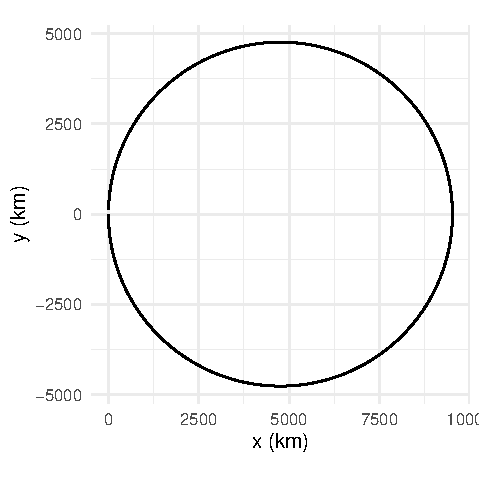
\includegraphics[width=0.45\linewidth,height=\textheight,keepaspectratio]{02-four-lines-to-an-orbit_files/figure-pdf/fig-earth-fixed-1.pdf}

}

\caption{\label{fig-earth-fixed}With zero total momentum, Earth's path
closes: a small circle around the center of mass, about 4,700 km from
the origin.}

\end{figure}%

Now Earth's path closes. For a Sun-planet system the same drift exists
and is a thousand times smaller, which is why the package's
\texttt{add\_sun()} puts the Sun at rest at the origin and nobody
notices. For a binary star, where the two masses are comparable, getting
the momentum right is the whole problem, and Chapter 9 builds the
Kepler-16 system from exactly this principle.

If you just want to \emph{look} at the Moon going around Earth without
thinking about the center of mass, there is a shortcut: re-center the
data on Earth after the fact.

\begin{Shaded}
\begin{Highlighting}[]
\NormalTok{moon }\SpecialCharTok{|\textgreater{}}
  \FunctionTok{shift\_reference\_frame}\NormalTok{(}\StringTok{"Earth"}\NormalTok{) }\SpecialCharTok{|\textgreater{}}
  \FunctionTok{plot\_orbits}\NormalTok{()}
\end{Highlighting}
\end{Shaded}

\texttt{shift\_reference\_frame()} subtracts Earth's position and
velocity from every body at every time step, which puts Earth at the
origin for the whole run. And if what you want is the drift gone without
re-running anything,
\texttt{shift\_reference\_frame(moon,\ "barycenter")} re-centers every
step on the pair's center of mass, which is where the system was sitting
all along. Chapter 10 is about what you can learn by doing this.

\section{Real bodies without looking anything
up}\label{real-bodies-without-looking-anything-up}

Typing masses, distances, and speeds works for any system you can
imagine. For the real solar system there is an easier way.
\texttt{add\_sun()} places the Sun at the origin at rest, and
\texttt{add\_planet()} places a planet using its real orbital elements
from the JPL DE440 ephemeris:

\begin{Shaded}
\begin{Highlighting}[]
\FunctionTok{create\_system}\NormalTok{() }\SpecialCharTok{|\textgreater{}}
  \FunctionTok{add\_sun}\NormalTok{() }\SpecialCharTok{|\textgreater{}}
  \FunctionTok{add\_planet}\NormalTok{(}\StringTok{"Mercury"}\NormalTok{, }\AttributeTok{parent =} \StringTok{"Sun"}\NormalTok{) }\SpecialCharTok{|\textgreater{}}
  \FunctionTok{add\_planet}\NormalTok{(}\StringTok{"Venus"}\NormalTok{,   }\AttributeTok{parent =} \StringTok{"Sun"}\NormalTok{) }\SpecialCharTok{|\textgreater{}}
  \FunctionTok{add\_planet}\NormalTok{(}\StringTok{"Earth"}\NormalTok{,   }\AttributeTok{parent =} \StringTok{"Sun"}\NormalTok{) }\SpecialCharTok{|\textgreater{}}
  \FunctionTok{add\_planet}\NormalTok{(}\StringTok{"Mars"}\NormalTok{,    }\AttributeTok{parent =} \StringTok{"Sun"}\NormalTok{) }\SpecialCharTok{|\textgreater{}}
  \FunctionTok{simulate\_system}\NormalTok{(}\AttributeTok{time\_step =}\NormalTok{ seconds\_per\_day, }\AttributeTok{duration =}\NormalTok{ seconds\_per\_year) }\SpecialCharTok{|\textgreater{}}
  \FunctionTok{plot\_orbits}\NormalTok{(}\AttributeTok{three\_d =} \ConstantTok{FALSE}\NormalTok{)}
\end{Highlighting}
\end{Shaded}

\begin{figure}[tbp]

\centering{

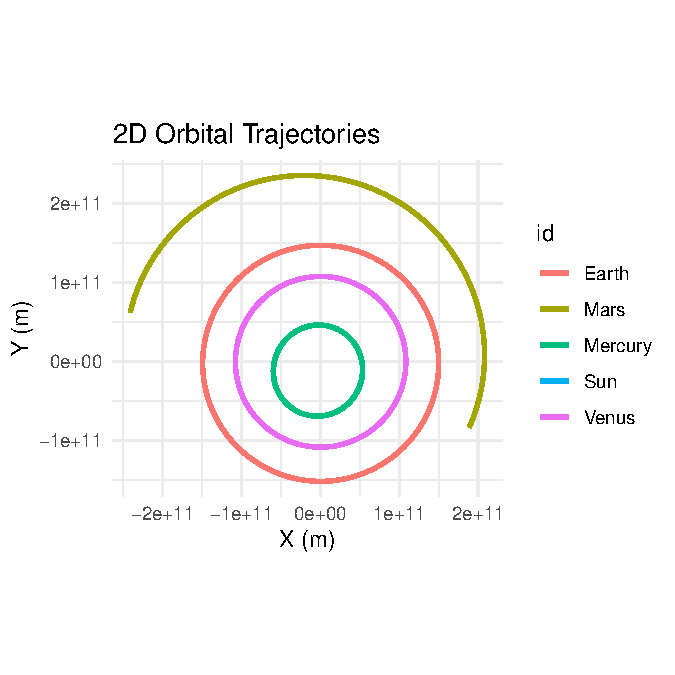
\includegraphics[width=0.7\linewidth,height=\textheight,keepaspectratio]{02-four-lines-to-an-orbit_files/figure-pdf/fig-inner-solar-system-1.pdf}

}

\caption{\label{fig-inner-solar-system}Mercury, Venus, Earth, and Mars
for one Earth year, placed from JPL orbital elements.}

\end{figure}%

\texttt{parent\ =\ "Sun"} tells \texttt{add\_planet()} which body the
orbit is around; the parent must already be in the system. Mercury
completes about four orbits in the time Earth completes one, and you can
see that its orbit is noticeably off-center: Mercury's eccentricity is
0.21, the largest of any planet.

\begin{tcolorbox}[enhanced jigsaw, arc=.35mm, bottomrule=.15mm, bottomtitle=1mm, breakable, colback=white, colbacktitle=quarto-callout-note-color!10!white, colframe=quarto-callout-note-color-frame, coltitle=black, left=2mm, leftrule=.75mm, opacityback=0, opacitybacktitle=0.6, rightrule=.15mm, title={Why three\_d = FALSE?}, titlerule=0mm, toprule=.15mm, toptitle=1mm]

The real planets' orbits are slightly tilted relative to one another, so
once you use \texttt{add\_planet()} the bodies have \(z\) motion.
\texttt{plot\_orbits()} notices and, by default, returns an interactive
3D plotly widget instead of a ggplot. That is the right thing on screen
and the wrong thing on paper, so throughout this book I pass
\texttt{three\_d\ =\ FALSE} for any system with real orbital elements.
On your own screen, leave it off and rotate the view.

\end{tcolorbox}

\texttt{load\_solar\_system()} builds the Sun, all eight planets, the
Moon, and Pluto in one call, and \texttt{remove\_body()} drops the ones
you do not want:

\begin{Shaded}
\begin{Highlighting}[]
\FunctionTok{load\_solar\_system}\NormalTok{() }\SpecialCharTok{|\textgreater{}}
  \FunctionTok{remove\_body}\NormalTok{(}\FunctionTok{c}\NormalTok{(}\StringTok{"Moon"}\NormalTok{, }\StringTok{"Pluto"}\NormalTok{)) }\SpecialCharTok{|\textgreater{}}
  \FunctionTok{simulate\_system}\NormalTok{(}\AttributeTok{time\_step =}\NormalTok{ seconds\_per\_day, }\AttributeTok{duration =}\NormalTok{ seconds\_per\_year }\SpecialCharTok{*} \DecValTok{12}\NormalTok{) }\SpecialCharTok{|\textgreater{}}
  \FunctionTok{plot\_orbits}\NormalTok{(}\AttributeTok{three\_d =} \ConstantTok{FALSE}\NormalTok{)}
\end{Highlighting}
\end{Shaded}

\begin{figure}[tbp]

\centering{

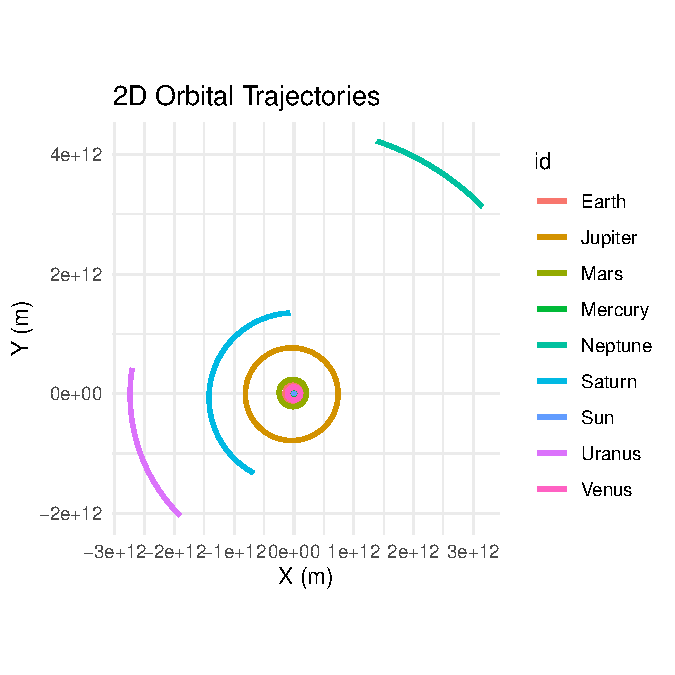
\includegraphics[width=0.7\linewidth,height=\textheight,keepaspectratio]{02-four-lines-to-an-orbit_files/figure-pdf/fig-outer-solar-system-1.pdf}

}

\caption{\label{fig-outer-solar-system}The whole solar system for twelve
years. The inner planets are a smudge at this scale; Neptune has
completed less than a tenth of an orbit.}

\end{figure}%

The Moon and Pluto are removed here for different reasons. Pluto's orbit
is large and does not change the picture. The Moon is removed because
simulating it correctly needs a time step of an hour or so, and a
twelve-year run at hourly steps is over a hundred thousand steps. One of
the first things you learn about N-body simulation is that the time step
is set by the \emph{fastest} orbit in the system, not the one you care
about. Chapter 5 explains why.

\section{Looking before you leap}\label{looking-before-you-leap}

A system is an object you can inspect before you run it. Printing one
shows the gravitational constant and the table of bodies:

\begin{Shaded}
\begin{Highlighting}[]
\NormalTok{sys }\OtherTok{\textless{}{-}} \FunctionTok{create\_system}\NormalTok{() }\SpecialCharTok{|\textgreater{}}
  \FunctionTok{add\_sun}\NormalTok{() }\SpecialCharTok{|\textgreater{}}
  \FunctionTok{add\_planet}\NormalTok{(}\StringTok{"Earth"}\NormalTok{, }\AttributeTok{parent =} \StringTok{"Sun"}\NormalTok{) }\SpecialCharTok{|\textgreater{}}
  \FunctionTok{add\_planet}\NormalTok{(}\StringTok{"Mars"}\NormalTok{,  }\AttributeTok{parent =} \StringTok{"Sun"}\NormalTok{)}

\NormalTok{sys}
\CommentTok{\#\textgreater{} ───────────────────────────────── orbit\_system ───────────────────────────────── }
\CommentTok{\#\textgreater{} G: 6.6743e{-}11 (standard)}
\CommentTok{\#\textgreater{} Bodies: 3}
\CommentTok{\#\textgreater{} }
\CommentTok{\#\textgreater{} \# A tibble: 3 x 8}
\CommentTok{\#\textgreater{}   id       mass             x             y            z      vx     vy    vz}
\CommentTok{\#\textgreater{}   \textless{}chr\textgreater{}   \textless{}dbl\textgreater{}         \textless{}dbl\textgreater{}         \textless{}dbl\textgreater{}        \textless{}dbl\textgreater{}   \textless{}dbl\textgreater{}  \textless{}dbl\textgreater{} \textless{}dbl\textgreater{}}
\CommentTok{\#\textgreater{} 1 Sun   1.99e30            0             0            0       0      0     0 }
\CommentTok{\#\textgreater{} 2 Earth 5.97e24 {-}32965585121. 143360295956.           0  {-}29520. {-}6788.    0 }
\CommentTok{\#\textgreater{} 3 Mars  6.42e23 188789951360. {-}83706961610. {-}6395443036.  10750. 24226.  243.}
\end{Highlighting}
\end{Shaded}

\texttt{get\_bodies()} returns that table as a plain tibble, which is
useful for checking that a hand-built system has the positions and
velocities you intended:

\begin{Shaded}
\begin{Highlighting}[]
\FunctionTok{get\_bodies}\NormalTok{(sys) }\SpecialCharTok{|\textgreater{}}
  \FunctionTok{mutate}\NormalTok{(}\AttributeTok{speed =} \FunctionTok{sqrt}\NormalTok{(vx}\SpecialCharTok{\^{}}\DecValTok{2} \SpecialCharTok{+}\NormalTok{ vy}\SpecialCharTok{\^{}}\DecValTok{2} \SpecialCharTok{+}\NormalTok{ vz}\SpecialCharTok{\^{}}\DecValTok{2}\NormalTok{)) }\SpecialCharTok{|\textgreater{}}
  \FunctionTok{select}\NormalTok{(id, speed)}
\CommentTok{\#\textgreater{} \# A tibble: 3 x 2}
\CommentTok{\#\textgreater{}   id     speed}
\CommentTok{\#\textgreater{}   \textless{}chr\textgreater{}  \textless{}dbl\textgreater{}}
\CommentTok{\#\textgreater{} 1 Sun       0 }
\CommentTok{\#\textgreater{} 2 Earth 30291.}
\CommentTok{\#\textgreater{} 3 Mars  26505.}
\end{Highlighting}
\end{Shaded}

Earth's initial speed is a little over its mean orbital speed of 29,780
m/s, because \texttt{add\_planet()} starts each body at periapsis (its
closest approach to the Sun), where it moves fastest. The \texttt{nu}
argument changes the starting point along the orbit; Chapter 7 covers it
with the rest of the orbital elements.

\section{Snapshots and animation}\label{snapshots-and-animation}

\texttt{plot\_orbits()} draws whole trajectories.
\texttt{plot\_system()} draws where everything is at one instant,
optionally with the trajectories drawn faintly behind:

\begin{Shaded}
\begin{Highlighting}[]
\NormalTok{inner }\OtherTok{\textless{}{-}} \FunctionTok{create\_system}\NormalTok{() }\SpecialCharTok{|\textgreater{}}
  \FunctionTok{add\_sun}\NormalTok{() }\SpecialCharTok{|\textgreater{}}
  \FunctionTok{add\_planet}\NormalTok{(}\StringTok{"Mercury"}\NormalTok{, }\AttributeTok{parent =} \StringTok{"Sun"}\NormalTok{) }\SpecialCharTok{|\textgreater{}}
  \FunctionTok{add\_planet}\NormalTok{(}\StringTok{"Venus"}\NormalTok{,   }\AttributeTok{parent =} \StringTok{"Sun"}\NormalTok{) }\SpecialCharTok{|\textgreater{}}
  \FunctionTok{add\_planet}\NormalTok{(}\StringTok{"Earth"}\NormalTok{,   }\AttributeTok{parent =} \StringTok{"Sun"}\NormalTok{) }\SpecialCharTok{|\textgreater{}}
  \FunctionTok{add\_planet}\NormalTok{(}\StringTok{"Mars"}\NormalTok{,    }\AttributeTok{parent =} \StringTok{"Sun"}\NormalTok{) }\SpecialCharTok{|\textgreater{}}
  \FunctionTok{simulate\_system}\NormalTok{(}\AttributeTok{time\_step =}\NormalTok{ seconds\_per\_day, }\AttributeTok{duration =}\NormalTok{ seconds\_per\_year)}

\FunctionTok{plot\_system}\NormalTok{(inner, }\AttributeTok{time =}\NormalTok{ seconds\_per\_day }\SpecialCharTok{*} \DecValTok{200}\NormalTok{, }\AttributeTok{trails =} \ConstantTok{TRUE}\NormalTok{, }\AttributeTok{three\_d =} \ConstantTok{FALSE}\NormalTok{)}
\end{Highlighting}
\end{Shaded}

\begin{figure}[tbp]

\centering{

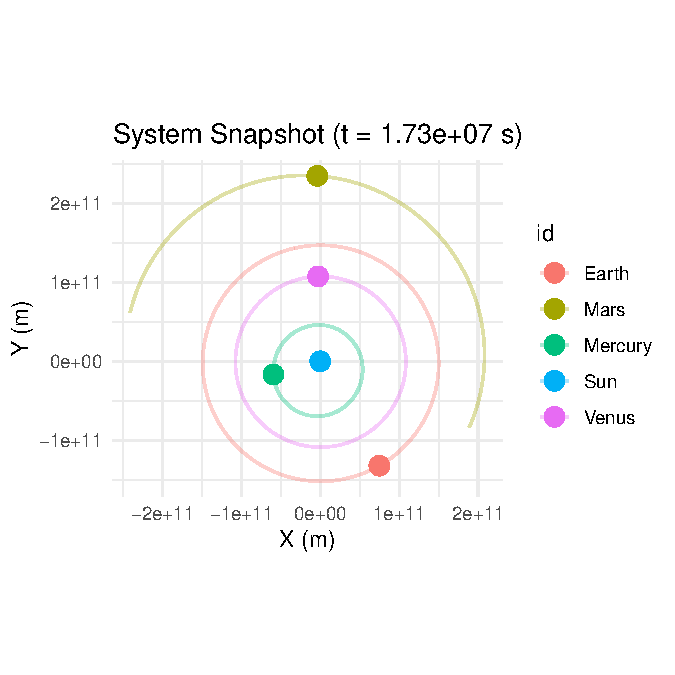
\includegraphics[width=0.7\linewidth,height=\textheight,keepaspectratio]{02-four-lines-to-an-orbit_files/figure-pdf/fig-snapshot-1.pdf}

}

\caption{\label{fig-snapshot}The inner solar system at day 200 of the
run, with trails.}

\end{figure}%

The \texttt{time} argument is in simulation seconds and snaps to the
nearest available step. A sequence of snapshots at different times is
how the printed book shows motion. On screen, use the animation:

\begin{Shaded}
\begin{Highlighting}[]
\FunctionTok{animate\_system}\NormalTok{(inner, }\AttributeTok{fps =} \DecValTok{15}\NormalTok{, }\AttributeTok{duration =} \DecValTok{6}\NormalTok{, }\AttributeTok{trails =} \ConstantTok{TRUE}\NormalTok{)}
\end{Highlighting}
\end{Shaded}

This samples the run down to \texttt{fps\ *\ duration} frames and
renders a GIF with gganimate (which you need to have installed, along
with gifski). Each body leaves a fading wake. Rendering takes tens of
seconds, so get the static plot right first.

\section{Saving and sharing}\label{saving-and-sharing}

\texttt{save\_system()} writes a system, bodies and all, to an
\texttt{.rds} file and \texttt{load\_system()} reads it back, so a
carefully tuned setup does not have to be rebuilt:

\begin{Shaded}
\begin{Highlighting}[]
\FunctionTok{save\_system}\NormalTok{(sys, }\StringTok{"earth{-}mars.rds"}\NormalTok{)}
\NormalTok{sys2 }\OtherTok{\textless{}{-}} \FunctionTok{load\_system}\NormalTok{(}\StringTok{"earth{-}mars.rds"}\NormalTok{)}
\end{Highlighting}
\end{Shaded}

\texttt{export\_bodies()} writes the body table to CSV, which is the
right format for handing initial conditions to someone who is not using
R:

\begin{Shaded}
\begin{Highlighting}[]
\FunctionTok{export\_bodies}\NormalTok{(sys, }\StringTok{"earth{-}mars{-}bodies.csv"}\NormalTok{)}
\end{Highlighting}
\end{Shaded}

The simulation output is just a tibble, so \texttt{readr::write\_csv()}
or \texttt{saveRDS()} handle it like any other data.

\part{Where the Physics Comes From}

\chapter{Newton's Law and the N-Body Problem}\label{sec-newton}

Everything orbitr does rests on one equation. This chapter writes it
down carefully, in the vector form the code actually uses, and then asks
the questions a careful reader should ask about it: why the mass of the
body being pulled drops out, why a planet can be treated as a point,
what the constant \(G\) is and how well it is known, and what the
computer does with the equation once it has it. By the end of the
chapter you will have written your own version of orbitr's inner loop in
plain R and checked it against the package.

\section{From the apple to the Moon}\label{from-the-apple-to-the-moon}

Newton's law of universal gravitation says that two point masses \(m_1\)
and \(m_2\) separated by a distance \(r\) attract each other with a
force of magnitude

\begin{equation}\protect\phantomsection\label{eq-newton-scalar}{
F = \frac{G\,m_1 m_2}{r^2}.
}\end{equation}

The force is along the line joining them, and it falls off as the
inverse square of the distance.

\begin{tcolorbox}[enhanced jigsaw, arc=.35mm, bottomrule=.15mm, bottomtitle=1mm, breakable, colback=white, colbacktitle=quarto-callout-note-color!10!white, colframe=quarto-callout-note-color-frame, coltitle=black, left=2mm, leftrule=.75mm, opacityback=0, opacitybacktitle=0.6, rightrule=.15mm, title={Where it comes from}, titlerule=0mm, toprule=.15mm, toptitle=1mm]

The inverse-square law was in the air in the 1670s. Robert Hooke, Edmond
Halley, and Christopher Wren all suspected that a force falling off as
\(1/r^2\) would produce Kepler's ellipses; none of them could prove it.
In 1684 Halley asked Newton what orbit such a force would produce.
Newton said an ellipse, that he had worked it out years before, and that
he had lost the calculation. He redid it, and the redoing grew into the
\emph{Principia} (Newton 1687).

The famous test is the Moon. If the same force that makes an apple fall
also holds the Moon in orbit, then since the Moon is about 60 Earth
radii away, its acceleration toward Earth should be \(1/60^2 = 1/3600\)
of \(g\). The acceleration needed to keep a body on a circle of radius
\(r\) with period \(T\) is \(4\pi^2 r/T^2\), and both numbers were known
in Newton's time. Here is the comparison with modern values:

\begin{Shaded}
\begin{Highlighting}[]
\NormalTok{R\_earth }\OtherTok{\textless{}{-}} \FloatTok{6.371e6}                           \CommentTok{\# m}
\NormalTok{g       }\OtherTok{\textless{}{-}} \FloatTok{9.81}                              \CommentTok{\# m/s\^{}2}
\NormalTok{T\_moon  }\OtherTok{\textless{}{-}} \FloatTok{27.32} \SpecialCharTok{*}\NormalTok{ seconds\_per\_day           }\CommentTok{\# sidereal month}

\NormalTok{g }\SpecialCharTok{*}\NormalTok{ (R\_earth }\SpecialCharTok{/}\NormalTok{ distance\_earth\_moon)}\SpecialCharTok{\^{}}\DecValTok{2}        \CommentTok{\# inverse{-}square prediction}
\CommentTok{\#\textgreater{} [1] 0.002694744}
\DecValTok{4} \SpecialCharTok{*}\NormalTok{ pi}\SpecialCharTok{\^{}}\DecValTok{2} \SpecialCharTok{*}\NormalTok{ distance\_earth\_moon }\SpecialCharTok{/}\NormalTok{ T\_moon}\SpecialCharTok{\^{}}\DecValTok{2}    \CommentTok{\# centripetal, from the orbit}
\CommentTok{\#\textgreater{} [1] 0.002723668}
\end{Highlighting}
\end{Shaded}

They agree to about one percent. The residual is mostly the Moon's own
mass: the orbit's period is set by the combined mass, \(G(M+m)\), which
is 1.2\% larger than \(GM\) alone. Chapter 4 makes this precise.
Newton's own first calculation, in the 1660s, used an inaccurate figure
for the size of the Earth and did not agree well; he returned to the
problem years later when Picard's survey gave a better one.

\end{tcolorbox}

\section{The law in vector form}\label{the-law-in-vector-form}

A simulation needs directions, not just magnitudes. Let \(\mathbf{r}_j\)
be the position vector of body \(j\). The vector from body \(j\) to body
\(k\) is \(\mathbf{r}_k - \mathbf{r}_j\), its length is
\(r_{jk} = |\mathbf{r}_k - \mathbf{r}_j|\), and the unit vector pointing
from \(j\) toward \(k\) is

\[
\hat{\mathbf{r}}_{jk} = \frac{\mathbf{r}_k - \mathbf{r}_j}{r_{jk}}.
\]

The force on \(j\) due to \(k\) points \emph{toward} \(k\) (gravity
attracts), so

\begin{equation}\protect\phantomsection\label{eq-newton-vector}{
\mathbf{F}_{jk} = \frac{G\,m_j m_k}{r_{jk}^2}\,\hat{\mathbf{r}}_{jk}.
}\end{equation}

Swapping \(j\) and \(k\) flips the unit vector and nothing else, so
\(\mathbf{F}_{kj} = -\mathbf{F}_{jk}\): Newton's third law is built in.
This is the fact behind the drifting Earth in Chapter 2. Because every
internal force comes in an equal and opposite pair, the total momentum
of a system of gravitating bodies never changes, no matter how
complicated the motion.

\section{Superposition: the N-body
acceleration}\label{superposition-the-n-body-acceleration}

Newton's second law gives the acceleration of body \(j\) from the net
force on it, \(m_j \ddot{\mathbf{r}}_j = \sum_k \mathbf{F}_{jk}\).
Gravitational forces add as vectors; the pull of the Sun on Earth does
not care that the Moon is also pulling. Summing
Equation~\ref{eq-newton-vector} over every other body and dividing by
\(m_j\),

\begin{equation}\protect\phantomsection\label{eq-nbody}{
\ddot{\mathbf{r}}_j = \sum_{k \neq j} \frac{G\,m_k}{r_{jk}^2}\,\hat{\mathbf{r}}_{jk}
= \sum_{k \neq j} G\,m_k\,\frac{\mathbf{r}_k - \mathbf{r}_j}{|\mathbf{r}_k - \mathbf{r}_j|^3}.
}\end{equation}

This is the equation. The first form is the one in the package
documentation; the second is the one the code uses, because it avoids
computing the unit vector separately. The cube in the denominator is one
power for turning the difference vector into a unit vector and two for
the inverse-square law.

Two things to notice.

\textbf{The mass of body \(j\) has cancelled.} The acceleration of a
body in a gravitational field does not depend on its own mass. A feather
and a hammer fall together; the International Space Station and an
astronaut floating inside it follow the same orbit. This is only true
because the \(m_j\) in Newton's second law (inertial mass, the
resistance to being accelerated) is the same quantity as the \(m_j\) in
the law of gravitation (gravitational mass, the thing that gravity pulls
on). Nothing in Newtonian mechanics requires those to be equal; they
just are. The equality has been tested to about one part in \(10^{15}\)
({Touboul et al.} 2022), and Einstein took it as the starting point of
general relativity. For the simulation it means something practical: a
body's mass matters for how it pulls on the others, but a test particle
of negligible mass follows exactly the same path it would with any other
negligible mass.

\textbf{The sum is over every pair.} With \(N\) bodies there are
\(N(N-1)\) ordered pairs, and each needs a subtraction, a norm, and a
division. Doubling the number of bodies quadruples the work. This
\(O(N^2)\) scaling is the single fact that dominates the design of every
N-body code ever written, and it is why orbitr's inner loop is in C++
(Chapter 15). For the handful of bodies in this book it is not a
problem.

\section{Why point masses are enough}\label{why-point-masses-are-enough}

Earth is not a point. It is a ball 12,742 km across, and every piece of
it pulls on the Moon from a slightly different direction and distance.
Why is it legitimate to write Equation~\ref{eq-nbody} with a single
\(\mathbf{r}_{\mathrm{Earth}}\)?

\begin{theorem}[Newton's shell
theorem]\protect\hypertarget{thm-shell}{}\label{thm-shell}

A spherically symmetric body attracts an external point mass exactly as
if all of its mass were concentrated at its center. A spherically
symmetric shell exerts no net gravitational force on a point mass
anywhere inside it.

\end{theorem}

Newton proved this geometrically in the \emph{Principia} (Book I,
Propositions 70 and 71), and he is often said to have delayed publishing
the theory of gravitation until he had the proof, since without it the
Moon test above is not justified. The modern proof takes three lines if
you know Gauss's law for gravity, which says that the flux of the
gravitational field \(\mathbf{g}\) through any closed surface is
proportional to the mass enclosed:

\[
\oint \mathbf{g}\cdot d\mathbf{A} = -4\pi G\,M_{\mathrm{enc}}.
\]

Take the surface to be a sphere of radius \(r\) centered on the body. By
symmetry, \(\mathbf{g}\) points radially and has the same magnitude
\(g(r)\) everywhere on the sphere, so the integral is
\(-g(r)\cdot 4\pi r^2\) (negative because the field points inward).
Hence \(g(r) = G M_{\mathrm{enc}}/r^2\), directed toward the center.
Outside the body, \(M_{\mathrm{enc}}\) is the whole mass, and the field
is that of a point mass. Inside a shell, \(M_{\mathrm{enc}} = 0\), and
the field vanishes.

So for any body whose mass is arranged in spherical shells, which is a
very good description of stars and planets, the point-mass equation is
not an approximation at all. It is exact, as long as the bodies do not
overlap.

Where it fails is instructive. Earth bulges at the equator by about 21
km because it spins; the extra mass there pulls satellites in low orbit
slightly off the point-mass prediction, and the orbits of GPS satellites
precess measurably because of it. Astronomers call the leading
correction \(J_2\). Two stars in a close binary raise tides on each
other and are not spherical either. orbitr ignores all of this, which is
the right choice for orbital distances and the wrong one for anything
skimming a surface. The package roadmap lists \(J_2\) as a possible
addition; Chapter 16 discusses what it would take.

\section{\texorpdfstring{Units, \(G\), and how well we know
it}{Units, G, and how well we know it}}\label{units-g-and-how-well-we-know-it}

Everything in orbitr is in SI: meters, kilograms, seconds. The
gravitational constant is

\begin{Shaded}
\begin{Highlighting}[]
\NormalTok{gravitational\_constant}
\CommentTok{\#\textgreater{} [1] 6.6743e{-}11}
\end{Highlighting}
\end{Shaded}

in \(\mathrm{m^3\,kg^{-1}\,s^{-2}}\). That is the CODATA 2018
recommended value, \(6.67430(15)\times10^{-11}\) (Tiesinga et al. 2021),
and the digits in parentheses are the uncertainty in the last two
places: about 2 parts in \(10^5\). By the standards of fundamental
constants that is terrible. The speed of light is exact by definition;
Planck's constant is now exact by definition; the fine-structure
constant is known to a few parts in \(10^{10}\). \(G\) is hard to
measure because gravity is so weak that laboratory experiments have to
detect the pull of a kilogram-scale mass on another, and because there
is no way to shield the apparatus from everything else.

The constant that astronomy actually uses is not \(G\) but the product
\(GM\) for each body, called the gravitational parameter and written
\(\mu\). For the Sun, \(GM_\odot\) is known to about one part in
\(10^{10}\), because it is what you get directly from fitting planetary
orbits and spacecraft trajectories, no laboratory required. When the
package reports the Sun's mass as \(1.989\times10^{30}\) kg, that number
is \(GM_\odot\) divided by a poorly known \(G\), and its uncertainty is
essentially the uncertainty in \(G\). None of this affects a simulation,
because the equations of motion only ever contain \(G\) and a mass
together. It does mean that if you ever compare a simulated orbital
period to a measured one at the fifth significant figure, the
discrepancy may be in \(G\), not in the integrator.

\section{The equations of motion as a
system}\label{the-equations-of-motion-as-a-system}

Equation~\ref{eq-nbody} is a second-order differential equation for each
of \(N\) bodies. A simulation does not work with second-order equations;
it works with a \emph{state} and a rule for advancing it. The state of
the system at time \(t\) is the list of all positions and velocities,

\[
\big(\mathbf{r}_1, \ldots, \mathbf{r}_N,\ \mathbf{v}_1, \ldots, \mathbf{v}_N\big),
\]

\(6N\) numbers in all. The rule for how the state changes is a pair of
first-order equations for each body,

\begin{equation}\protect\phantomsection\label{eq-state}{
\dot{\mathbf{r}}_j = \mathbf{v}_j, \qquad
\dot{\mathbf{v}}_j = \mathbf{a}_j(\mathbf{r}_1, \ldots, \mathbf{r}_N),
}\end{equation}

where \(\mathbf{a}_j\) is the right-hand side of
Equation~\ref{eq-nbody}. The accelerations depend only on positions, not
on velocities. That is a special feature of gravity (and of any force
that comes from a potential), and Chapter 5 will show that the best
integrators exploit it.

Here is the structure of every N-body code, including this one, in
pseudo-code:

\begin{verbatim}
state <- initial positions and velocities
for each time step:
    a     <- accelerations(state)        # the N-body sum, all pairs
    state <- advance(state, a, dt)       # the integrator
    record state
\end{verbatim}

The \texttt{accelerations()} function is the physics. The
\texttt{advance()} function is the numerics. orbitr keeps them separate,
and so will this book: this chapter is about the first function, Chapter
5 is about the second.

\section{Writing the acceleration
yourself}\label{writing-the-acceleration-yourself}

The best way to be sure what Equation~\ref{eq-nbody} says is to
implement it. Here it is in plain R, with no attempt at speed:

\begin{Shaded}
\begin{Highlighting}[]
\NormalTok{accelerations }\OtherTok{\textless{}{-}} \ControlFlowTok{function}\NormalTok{(bodies, }\AttributeTok{G =}\NormalTok{ gravitational\_constant) \{}
\NormalTok{  n   }\OtherTok{\textless{}{-}} \FunctionTok{nrow}\NormalTok{(bodies)}
\NormalTok{  pos }\OtherTok{\textless{}{-}} \FunctionTok{as.matrix}\NormalTok{(bodies[, }\FunctionTok{c}\NormalTok{(}\StringTok{"x"}\NormalTok{, }\StringTok{"y"}\NormalTok{, }\StringTok{"z"}\NormalTok{)])}
\NormalTok{  a   }\OtherTok{\textless{}{-}} \FunctionTok{matrix}\NormalTok{(}\DecValTok{0}\NormalTok{, }\AttributeTok{nrow =}\NormalTok{ n, }\AttributeTok{ncol =} \DecValTok{3}\NormalTok{)}
  \ControlFlowTok{for}\NormalTok{ (j }\ControlFlowTok{in} \FunctionTok{seq\_len}\NormalTok{(n)) \{}
    \ControlFlowTok{for}\NormalTok{ (k }\ControlFlowTok{in} \FunctionTok{seq\_len}\NormalTok{(n)) \{}
      \ControlFlowTok{if}\NormalTok{ (j }\SpecialCharTok{==}\NormalTok{ k) }\ControlFlowTok{next}
\NormalTok{      d }\OtherTok{\textless{}{-}}\NormalTok{ pos[k, ] }\SpecialCharTok{{-}}\NormalTok{ pos[j, ]         }\CommentTok{\# vector from j toward k}
\NormalTok{      r }\OtherTok{\textless{}{-}} \FunctionTok{sqrt}\NormalTok{(}\FunctionTok{sum}\NormalTok{(d}\SpecialCharTok{\^{}}\DecValTok{2}\NormalTok{))              }\CommentTok{\# distance}
\NormalTok{      a[j, ] }\OtherTok{\textless{}{-}}\NormalTok{ a[j, ] }\SpecialCharTok{+}\NormalTok{ G }\SpecialCharTok{*}\NormalTok{ bodies}\SpecialCharTok{$}\NormalTok{mass[k] }\SpecialCharTok{*}\NormalTok{ d }\SpecialCharTok{/}\NormalTok{ r}\SpecialCharTok{\^{}}\DecValTok{3}
\NormalTok{    \}}
\NormalTok{  \}}
  \FunctionTok{tibble}\NormalTok{(}\AttributeTok{id =}\NormalTok{ bodies}\SpecialCharTok{$}\NormalTok{id, }\AttributeTok{ax =}\NormalTok{ a[, }\DecValTok{1}\NormalTok{], }\AttributeTok{ay =}\NormalTok{ a[, }\DecValTok{2}\NormalTok{], }\AttributeTok{az =}\NormalTok{ a[, }\DecValTok{3}\NormalTok{])}
\NormalTok{\}}
\end{Highlighting}
\end{Shaded}

The double loop runs over all ordered pairs \((j, k)\) with
\(j \neq k\). For each pair it forms the difference vector, its length,
and the term in the sum. \texttt{bodies} is any data frame with columns
\texttt{id}, \texttt{mass}, \texttt{x}, \texttt{y}, \texttt{z}, which is
exactly what \texttt{get\_bodies()} returns:

\begin{Shaded}
\begin{Highlighting}[]
\NormalTok{em }\OtherTok{\textless{}{-}} \FunctionTok{create\_system}\NormalTok{() }\SpecialCharTok{|\textgreater{}}
  \FunctionTok{add\_body}\NormalTok{(}\StringTok{"Earth"}\NormalTok{, }\AttributeTok{mass =}\NormalTok{ mass\_earth) }\SpecialCharTok{|\textgreater{}}
  \FunctionTok{add\_body}\NormalTok{(}\StringTok{"Moon"}\NormalTok{,  }\AttributeTok{mass =}\NormalTok{ mass\_moon, }\AttributeTok{x =}\NormalTok{ distance\_earth\_moon, }\AttributeTok{vy =}\NormalTok{ speed\_moon)}

\FunctionTok{accelerations}\NormalTok{(}\FunctionTok{get\_bodies}\NormalTok{(em))}
\CommentTok{\#\textgreater{} \# A tibble: 2 x 4}
\CommentTok{\#\textgreater{}   id            ax    ay    az}
\CommentTok{\#\textgreater{}   \textless{}chr\textgreater{}      \textless{}dbl\textgreater{} \textless{}dbl\textgreater{} \textless{}dbl\textgreater{}}
\CommentTok{\#\textgreater{} 1 Earth  0.0000332     0     0}
\CommentTok{\#\textgreater{} 2 Moon  {-}0.00270       0     0}
\end{Highlighting}
\end{Shaded}

The Moon's acceleration is in the \(-x\) direction, toward Earth, with
magnitude \(G M_{\mathrm{Earth}}/r^2\):

\begin{Shaded}
\begin{Highlighting}[]
\NormalTok{gravitational\_constant }\SpecialCharTok{*}\NormalTok{ mass\_earth }\SpecialCharTok{/}\NormalTok{ distance\_earth\_moon}\SpecialCharTok{\^{}}\DecValTok{2}
\CommentTok{\#\textgreater{} [1] 0.002697483}
\end{Highlighting}
\end{Shaded}

and Earth's is in the \(+x\) direction, toward the Moon, smaller by the
mass ratio \(m_{\mathrm{Moon}}/M_{\mathrm{Earth}} \approx 1/81\). Equal
and opposite \emph{forces}; unequal accelerations.

Now a check against the package. The package's output does not include
accelerations, but it does include velocities at every step, and over
one hour the velocity change of the Moon should be close to
\(\mathbf{a}\,\Delta t\):

\begin{Shaded}
\begin{Highlighting}[]
\NormalTok{sim }\OtherTok{\textless{}{-}} \FunctionTok{simulate\_system}\NormalTok{(em, }\AttributeTok{time\_step =}\NormalTok{ seconds\_per\_hour,}
                       \AttributeTok{duration =}\NormalTok{ seconds\_per\_hour)}

\NormalTok{sim }\SpecialCharTok{|\textgreater{}}
  \FunctionTok{filter}\NormalTok{(id }\SpecialCharTok{==} \StringTok{"Moon"}\NormalTok{) }\SpecialCharTok{|\textgreater{}}
  \FunctionTok{summarise}\NormalTok{(}\AttributeTok{dvx\_per\_second =} \FunctionTok{diff}\NormalTok{(vx) }\SpecialCharTok{/}\NormalTok{ seconds\_per\_hour)}
\CommentTok{\#\textgreater{} \# A tibble: 1 x 1}
\CommentTok{\#\textgreater{}   dvx\_per\_second}
\CommentTok{\#\textgreater{}            \textless{}dbl\textgreater{}}
\CommentTok{\#\textgreater{} 1       {-}0.00270}
\end{Highlighting}
\end{Shaded}

That is the \(x\) acceleration computed above, to about four significant
figures. (It is not exact because the acceleration changes slightly
during the hour as the Moon moves; the integrator uses the average of
the accelerations at the start and end of the step, which is one of the
things that makes it good.)

\section{A three-body example}\label{a-three-body-example}

With three bodies the sums in Equation~\ref{eq-nbody} have two terms
each. Put the Sun at the origin, Earth at 1 AU, and the Moon 384,400 km
beyond Earth, and ask how hard the Sun pulls on the Moon compared to how
hard Earth does:

\begin{Shaded}
\begin{Highlighting}[]
\NormalTok{sem }\OtherTok{\textless{}{-}} \FunctionTok{create\_system}\NormalTok{() }\SpecialCharTok{|\textgreater{}}
  \FunctionTok{add\_sun}\NormalTok{() }\SpecialCharTok{|\textgreater{}}
  \FunctionTok{add\_body}\NormalTok{(}\StringTok{"Earth"}\NormalTok{, }\AttributeTok{mass =}\NormalTok{ mass\_earth, }\AttributeTok{x =}\NormalTok{ distance\_earth\_sun) }\SpecialCharTok{|\textgreater{}}
  \FunctionTok{add\_body}\NormalTok{(}\StringTok{"Moon"}\NormalTok{,  }\AttributeTok{mass =}\NormalTok{ mass\_moon,}
           \AttributeTok{x =}\NormalTok{ distance\_earth\_sun }\SpecialCharTok{+}\NormalTok{ distance\_earth\_moon)}

\NormalTok{a\_sun\_on\_moon   }\OtherTok{\textless{}{-}}\NormalTok{ gravitational\_constant }\SpecialCharTok{*}\NormalTok{ mass\_sun }\SpecialCharTok{/}
\NormalTok{                   (distance\_earth\_sun }\SpecialCharTok{+}\NormalTok{ distance\_earth\_moon)}\SpecialCharTok{\^{}}\DecValTok{2}
\NormalTok{a\_earth\_on\_moon }\OtherTok{\textless{}{-}}\NormalTok{ gravitational\_constant }\SpecialCharTok{*}\NormalTok{ mass\_earth }\SpecialCharTok{/}
\NormalTok{                   distance\_earth\_moon}\SpecialCharTok{\^{}}\DecValTok{2}

\NormalTok{a\_sun\_on\_moon }\SpecialCharTok{/}\NormalTok{ a\_earth\_on\_moon}
\CommentTok{\#\textgreater{} [1] 2.187709}
\end{Highlighting}
\end{Shaded}

The Sun pulls on the Moon more than twice as hard as Earth does. This
surprises almost everyone the first time. The Moon orbits Earth not
because Earth's pull is stronger but because Earth and the Moon are
\emph{both} falling toward the Sun together, at nearly the same rate;
what keeps the Moon bound to Earth is the small \emph{difference}
between the Sun's pull on the two of them. Seen from the Sun, the Moon's
path is a slightly wobbly ellipse that is everywhere concave toward the
Sun. Chapter 10 draws it.

The full acceleration of the Moon is the vector sum of both terms, and
our function gets it right with no changes:

\begin{Shaded}
\begin{Highlighting}[]
\FunctionTok{accelerations}\NormalTok{(}\FunctionTok{get\_bodies}\NormalTok{(sem)) }\SpecialCharTok{|\textgreater{}}
  \FunctionTok{filter}\NormalTok{(id }\SpecialCharTok{==} \StringTok{"Moon"}\NormalTok{)}
\CommentTok{\#\textgreater{} \# A tibble: 1 x 4}
\CommentTok{\#\textgreater{}   id          ax    ay    az}
\CommentTok{\#\textgreater{}   \textless{}chr\textgreater{}    \textless{}dbl\textgreater{} \textless{}dbl\textgreater{} \textless{}dbl\textgreater{}}
\CommentTok{\#\textgreater{} 1 Moon  {-}0.00860     0     0}
\end{Highlighting}
\end{Shaded}

\section{What the engine does
differently}\label{what-the-engine-does-differently}

The function above is correct and slow. Each call does \(N(N-1)\)
iterations of interpreted R, and a simulation calls it once or twice per
step for hundreds of thousands of steps. The package's pure-R fallback
vectorizes the same computation with matrix outer products so that R
does the loop in compiled code internally; its C++ engine writes the
double loop directly in C++ and runs about as fast as the hardware
allows. Both compute exactly Equation~\ref{eq-nbody}, with one small
addition: an optional softening length \(\varepsilon\) that replaces
\(r^3\) in the denominator with \((r^2 + \varepsilon^2)^{3/2}\). With
\(\varepsilon = 0\), the default, there is no difference. Chapter 6
explains what softening is for.

\begin{tcolorbox}[enhanced jigsaw, arc=.35mm, bottomrule=.15mm, bottomtitle=1mm, breakable, colback=white, colbacktitle=quarto-callout-tip-color!10!white, colframe=quarto-callout-tip-color-frame, coltitle=black, left=2mm, leftrule=.75mm, opacityback=0, opacitybacktitle=0.6, rightrule=.15mm, title={Key results}, titlerule=0mm, toprule=.15mm, toptitle=1mm]

\begin{itemize}
\tightlist
\item
  The acceleration of body \(j\) is
  \(\displaystyle \ddot{\mathbf{r}}_j = \sum_{k \neq j} G\,m_k\,\frac{\mathbf{r}_k - \mathbf{r}_j}{|\mathbf{r}_k - \mathbf{r}_j|^3}\).
  It does not depend on \(m_j\).
\item
  Internal forces come in equal and opposite pairs, so total momentum is
  conserved: the center of mass of any isolated system moves at constant
  velocity.
\item
  A spherically symmetric body gravitates exactly like a point mass at
  its center (shell theorem).
\item
  The computational cost grows as \(N^2\).
\end{itemize}

\end{tcolorbox}

\chapter{The Two-Body Problem, Solved by Hand}\label{sec-two-body}

The package documentation hands you a handful of formulas. The
circular-orbit speed is \(\sqrt{GM/r}\); escape speed is \(\sqrt{2}\)
times that; an orbit's period is \(2\pi\sqrt{a^3/\mu}\); the distance
from the parent at true anomaly \(\nu\) is \(a(1-e^2)/(1+e\cos\nu)\).
Every one of them is true, and every one of them follows from Newton's
law in a few lines of vector algebra. This chapter does the algebra. It
is the one place in the book where the derivations come first and the
code comes second, and it will repay the effort: these are the formulas
you will use to set up every system in Part III.

The strategy is the physicist's standard one. First find the quantities
that \emph{do not change} as the bodies move, the conserved quantities.
Then use them to pin down the shape of the orbit without ever
integrating anything. Along the way, Kepler's three laws drop out as
consequences.

\section{Two bodies become one}\label{two-bodies-become-one}

Take two point masses, \(m_1\) at \(\mathbf{r}_1\) and \(m_2\) at
\(\mathbf{r}_2\), with nothing else in the universe. From
Equation~\ref{eq-nbody},

\[
\ddot{\mathbf{r}}_1 = G m_2 \frac{\mathbf{r}_2 - \mathbf{r}_1}{r^3}, \qquad
\ddot{\mathbf{r}}_2 = G m_1 \frac{\mathbf{r}_1 - \mathbf{r}_2}{r^3},
\]

where \(r = |\mathbf{r}_2 - \mathbf{r}_1|\). Subtract the first from the
second. Writing \(\mathbf{r} = \mathbf{r}_2 - \mathbf{r}_1\) for the
\emph{relative} position of body 2 as seen from body 1,

\begin{equation}\protect\phantomsection\label{eq-relative}{
\ddot{\mathbf{r}} = -\frac{\mu}{r^3}\,\mathbf{r}, \qquad \mu = G(m_1 + m_2).
}\end{equation}

Two coupled equations in six coordinates have become one equation in
three. It says the relative position vector accelerates toward the
origin as if there were a single fixed mass \(m_1 + m_2\) sitting there.
The combination \(\mu = G(m_1+m_2)\) is called the gravitational
parameter, and it is the only combination of \(G\) and the masses that
the relative motion knows about.

What happened to the other three coordinates? Add \(m_1\) times the
first equation to \(m_2\) times the second: the right-hand sides cancel,
so the center of mass
\(\mathbf{R} = (m_1\mathbf{r}_1 + m_2\mathbf{r}_2)/(m_1+m_2)\) has
\(\ddot{\mathbf{R}} = 0\). It moves in a straight line at constant
velocity, which is the drift we met in Chapter 2. Given \(\mathbf{R}\)
and \(\mathbf{r}\), the individual positions are

\begin{equation}\protect\phantomsection\label{eq-individual}{
\mathbf{r}_1 = \mathbf{R} - \frac{m_2}{m_1+m_2}\,\mathbf{r}, \qquad
\mathbf{r}_2 = \mathbf{R} + \frac{m_1}{m_1+m_2}\,\mathbf{r}.
}\end{equation}

Both bodies trace the same shape of orbit around the center of mass,
scaled by the mass ratio. In Chapter 2's fixed Earth-Moon system,
Earth's little circle had a radius
\(m_{\mathrm{Moon}}/(m_{\mathrm{Earth}}+m_{\mathrm{Moon}}) \approx 1/82\)
of the Moon's.

When one body is much heavier, \(m_1 \gg m_2\), two things happen at
once: \(\mu \approx G m_1\), and \(\mathbf{r}_1 \approx \mathbf{R}\), so
the heavy body sits essentially at the center of mass and the light body
orbits it. That is the ``fixed central body'' picture of the two-body
vignette, and the approximation is excellent for the Sun and any planet
(the Sun outweighs Jupiter a thousand to one) and merely good for Earth
and the Moon, where the correction is 1.2\%. From here on the derivation
is exact for the relative motion; whether you then set \(\mu = GM\) or
\(\mu = G(M+m)\) is a choice about how much precision you need.

\section{Angular momentum is conserved, and the orbit is
flat}\label{angular-momentum-is-conserved-and-the-orbit-is-flat}

Define the \emph{specific angular momentum} (angular momentum per unit
mass) of the relative motion,

\[
\mathbf{h} = \mathbf{r} \times \dot{\mathbf{r}}.
\]

Differentiate it using the product rule:

\[
\dot{\mathbf{h}} = \dot{\mathbf{r}} \times \dot{\mathbf{r}} + \mathbf{r} \times \ddot{\mathbf{r}}
= \mathbf{0} + \mathbf{r} \times \left(-\frac{\mu}{r^3}\mathbf{r}\right) = \mathbf{0}.
\]

The first term is a vector crossed with itself and the second is
\(\mathbf{r}\) crossed with a multiple of \(\mathbf{r}\); both vanish.
So \(\mathbf{h}\) is a constant of the motion. This works for \emph{any}
force directed along \(\mathbf{r}\), not just inverse-square: it is a
consequence of the force being central.

Two consequences follow immediately. Since \(\mathbf{h}\) is
perpendicular to both \(\mathbf{r}\) and \(\dot{\mathbf{r}}\) at every
instant, and \(\mathbf{h}\) never changes, the position and velocity are
confined forever to the plane perpendicular to \(\mathbf{h}\).
\textbf{Every two-body orbit is planar.} And the magnitude
\(h = |\mathbf{r}\times\dot{\mathbf{r}}|\) is constant. In a small time
\(dt\) the position vector sweeps out a thin triangle with sides
\(\mathbf{r}\) and \(\dot{\mathbf{r}}\,dt\), whose area is half the
magnitude of their cross product:

\begin{equation}\protect\phantomsection\label{eq-areal}{
\frac{dA}{dt} = \frac{1}{2}\,|\mathbf{r} \times \dot{\mathbf{r}}| = \frac{h}{2}.
}\end{equation}

The line from the central body to the orbiting one sweeps out equal
areas in equal times. That is \textbf{Kepler's second law}, and it took
one line.

\section{Energy is conserved}\label{energy-is-conserved}

Now dot Equation~\ref{eq-relative} with the velocity:

\[
\dot{\mathbf{r}}\cdot\ddot{\mathbf{r}} = -\frac{\mu}{r^3}\,\mathbf{r}\cdot\dot{\mathbf{r}}.
\]

The left side is
\(\frac{d}{dt}\left(\tfrac12 \dot{\mathbf{r}}\cdot\dot{\mathbf{r}}\right) = \frac{d}{dt}\left(\tfrac12 v^2\right)\).
For the right side, note that \(r^2 = \mathbf{r}\cdot\mathbf{r}\), so
\(2r\dot{r} = 2\,\mathbf{r}\cdot\dot{\mathbf{r}}\) and
\(\mathbf{r}\cdot\dot{\mathbf{r}} = r\dot{r}\). Then
\(-\mu\,\mathbf{r}\cdot\dot{\mathbf{r}}/r^3 = -\mu\dot{r}/r^2 = \frac{d}{dt}(\mu/r)\).
Moving everything to one side,

\begin{equation}\protect\phantomsection\label{eq-energy}{
\frac{d}{dt}\left(\frac{v^2}{2} - \frac{\mu}{r}\right) = 0, \qquad
\varepsilon \equiv \frac{v^2}{2} - \frac{\mu}{r} = \text{const}.
}\end{equation}

\(\varepsilon\) is the \emph{specific orbital energy}: kinetic energy
per unit mass plus gravitational potential energy per unit mass. If
\(\varepsilon < 0\) the body cannot reach \(r = \infty\) (it would need
negative kinetic energy there), so it is bound. If \(\varepsilon \ge 0\)
it can, and it escapes.

Chapter 12 turns both of these conservation laws into diagnostics: a
simulation that lets \(\varepsilon\) or \(\mathbf{h}\) drift is a
simulation with a problem.

\section{The orbit equation}\label{the-orbit-equation}

Here is the step that makes the whole chapter work. Conservation of
\(\mathbf{h}\) and \(\varepsilon\) constrains the motion but does not by
itself give the shape of the path. For the inverse-square force, and
essentially only for it, there is a \emph{third} conserved vector, and
it hands you the orbit directly.

Start from the time derivative of \(\dot{\mathbf{r}}\times\mathbf{h}\).
Since \(\mathbf{h}\) is constant,

\[
\frac{d}{dt}\left(\dot{\mathbf{r}}\times\mathbf{h}\right) = \ddot{\mathbf{r}}\times\mathbf{h}
= -\frac{\mu}{r^3}\,\mathbf{r}\times(\mathbf{r}\times\dot{\mathbf{r}}).
\]

Expand the triple product with the identity
\(\mathbf{a}\times(\mathbf{b}\times\mathbf{c}) = \mathbf{b}(\mathbf{a}\cdot\mathbf{c}) - \mathbf{c}(\mathbf{a}\cdot\mathbf{b})\):

\[
\mathbf{r}\times(\mathbf{r}\times\dot{\mathbf{r}}) = \mathbf{r}\,(\mathbf{r}\cdot\dot{\mathbf{r}}) - \dot{\mathbf{r}}\,r^2
= \mathbf{r}\,r\dot{r} - \dot{\mathbf{r}}\,r^2,
\]

so

\[
\frac{d}{dt}\left(\dot{\mathbf{r}}\times\mathbf{h}\right)
= \mu\left(\frac{\dot{\mathbf{r}}}{r} - \frac{\dot{r}\,\mathbf{r}}{r^2}\right)
= \mu\,\frac{d}{dt}\left(\frac{\mathbf{r}}{r}\right).
\]

The last equality is just the quotient rule applied to \(\mathbf{r}/r\).
Both sides are total time derivatives, so their difference is a constant
vector. Divide by \(\mu\) and call the constant \(\mathbf{e}\):

\begin{equation}\protect\phantomsection\label{eq-ecc-vector}{
\mathbf{e} = \frac{\dot{\mathbf{r}}\times\mathbf{h}}{\mu} - \frac{\mathbf{r}}{r}.
}\end{equation}

This is the \emph{eccentricity vector} (also called the
Laplace-Runge-Lenz vector, in various normalizations). It lies in the
orbital plane, because both terms do. To see what it means, take its dot
product with \(\mathbf{r}\). The first term gives
\(\mathbf{r}\cdot(\dot{\mathbf{r}}\times\mathbf{h})/\mu = \mathbf{h}\cdot(\mathbf{r}\times\dot{\mathbf{r}})/\mu = h^2/\mu\),
using the cyclic property of the scalar triple product; the second gives
\(-r\). If \(\nu\) is the angle between \(\mathbf{e}\) and
\(\mathbf{r}\), the dot product is also \(e\,r\cos\nu\). So

\begin{equation}\protect\phantomsection\label{eq-orbit}{
e\,r\cos\nu = \frac{h^2}{\mu} - r
\quad\Longrightarrow\quad
r = \frac{h^2/\mu}{1 + e\cos\nu}.
}\end{equation}

This is the \textbf{orbit equation}: the distance from the central body
as a function of the angle \(\nu\) measured from the direction of
\(\mathbf{e}\). The quantity \(p = h^2/\mu\) is called the semi-latus
rectum, and \(e = |\mathbf{e}|\) is the eccentricity. The distance \(r\)
is smallest when \(\cos\nu = 1\), so \(\mathbf{e}\) points toward the
point of closest approach, the \emph{periapsis}, and \(\nu\), the
\emph{true anomaly}, is the angle from periapsis.
Equation~\ref{eq-orbit} is a conic section with one focus at the origin:

\begin{longtable}[]{@{}llll@{}}
\caption{The four kinds of two-body
orbit.}\label{tbl-conics}\tabularnewline
\toprule\noalign{}
\(e\) & \(\varepsilon\) & shape & \(r_{\max}\) \\
\midrule\noalign{}
\endfirsthead
\toprule\noalign{}
\(e\) & \(\varepsilon\) & shape & \(r_{\max}\) \\
\midrule\noalign{}
\endhead
\bottomrule\noalign{}
\endlastfoot
\(0\) & \(-\mu^2/2h^2\) & circle & \(= r_{\min}\) \\
\(0 < e < 1\) & \(< 0\) & ellipse & finite \\
\(1\) & \(0\) & parabola & \(\infty\) \\
\(> 1\) & \(> 0\) & hyperbola & \(\infty\) \\
\end{longtable}

Bound orbits are ellipses with the central body at a focus. That is
\textbf{Kepler's first law}, and it has now been derived from the
inverse-square law, which is the thing Halley asked Newton about in
1684.

The relation between \(e\) and \(\varepsilon\) in the table comes from
squaring Equation~\ref{eq-ecc-vector}. Since
\(\dot{\mathbf{r}} \perp \mathbf{h}\),
\(|\dot{\mathbf{r}}\times\mathbf{h}| = vh\), and the cross term is
\(-2\,\mathbf{r}\cdot(\dot{\mathbf{r}}\times\mathbf{h})/(\mu r) = -2h^2/(\mu r)\),
so

\begin{equation}\protect\phantomsection\label{eq-e-energy}{
e^2 = \frac{v^2 h^2}{\mu^2} - \frac{2h^2}{\mu r} + 1 = 1 + \frac{2\varepsilon h^2}{\mu^2}.
}\end{equation}

Negative energy means \(e<1\): bound orbits are ellipses, as the table
says.

\begin{tcolorbox}[enhanced jigsaw, arc=.35mm, bottomrule=.15mm, bottomtitle=1mm, breakable, colback=white, colbacktitle=quarto-callout-note-color!10!white, colframe=quarto-callout-note-color-frame, coltitle=black, left=2mm, leftrule=.75mm, opacityback=0, opacitybacktitle=0.6, rightrule=.15mm, title={Where it comes from}, titlerule=0mm, toprule=.15mm, toptitle=1mm]

Kepler extracted his first two laws from Tycho Brahe's observations of
Mars, published in \emph{Astronomia Nova} in 1609 (Kepler 1609), and the
third from the periods and distances of all the planets, published in
\emph{Harmonices Mundi} in 1619 (Kepler 1619). He had no theory of why;
he had tried circles and epicycles for years and the data would not fit.
Newton's \emph{Principia} (Newton 1687) showed that all three laws
follow from an inverse-square force (Book I, Propositions 11 to 15),
using geometry rather than vectors. The vector form here is the standard
modern one; Goldstein (Goldstein et al. 2002) and Bate, Mueller, and
White (Bate et al. 1971) both present it, and the eccentricity vector is
the starting point of every algorithm that turns a position and velocity
into orbital elements, including the one in Chapter 7.

\end{tcolorbox}

\section{The geometry of an ellipse}\label{the-geometry-of-an-ellipse}

An ellipse has a longest diameter, the major axis, of length \(2a\);
\(a\) is the semi-major axis. From Equation~\ref{eq-orbit} the nearest
and farthest points are at \(\nu = 0\) and \(\nu = \pi\):

\[
r_p = \frac{p}{1+e}, \qquad r_a = \frac{p}{1-e}, \qquad a = \frac{r_p + r_a}{2} = \frac{p}{1-e^2}.
\]

So \(p = a(1-e^2)\), and the orbit equation takes the form the package
uses:

\begin{equation}\protect\phantomsection\label{eq-orbit-a}{
r = \frac{a(1-e^2)}{1+e\cos\nu}, \qquad r_p = a(1-e), \qquad r_a = a(1+e).
}\end{equation}

The semi-minor axis is \(b = a\sqrt{1-e^2}\). Two more facts fall out of
these. First, given any two-body orbit, you can read off its
eccentricity from its extreme distances alone:

\begin{equation}\protect\phantomsection\label{eq-e-from-extremes}{
e = \frac{r_a - r_p}{r_a + r_p}.
}\end{equation}

Second, substituting \(h^2 = \mu p = \mu a(1-e^2)\) into
Equation~\ref{eq-e-energy} and simplifying (try it; everything but one
factor cancels) gives the energy in terms of the size of the orbit
alone:

\begin{equation}\protect\phantomsection\label{eq-energy-a}{
\varepsilon = -\frac{\mu}{2a}.
}\end{equation}

The energy of an orbit depends only on its semi-major axis, not on its
eccentricity. A circle of radius \(a\) and a needle-thin ellipse of
semi-major axis \(a\) have the same energy.

\section{Vis-viva, circular speed, and escape
speed}\label{vis-viva-circular-speed-and-escape-speed}

Put Equation~\ref{eq-energy-a} into the definition of \(\varepsilon\)
and solve for the speed:

\begin{equation}\protect\phantomsection\label{eq-vis-viva}{
v^2 = \mu\left(\frac{2}{r} - \frac{1}{a}\right).
}\end{equation}

This is the \emph{vis-viva} equation (Latin for ``living force,'' an old
name for kinetic energy). It gives the speed at any distance \(r\) along
an orbit of semi-major axis \(a\), and it is the formula you want
whenever you know where a body is and need to know how fast it should be
going.

Two special cases are the ones the documentation quotes. On a circular
orbit, \(r = a\) always, so

\begin{equation}\protect\phantomsection\label{eq-v-circ}{
v_{\mathrm{circ}} = \sqrt{\frac{\mu}{r}}.
}\end{equation}

On a parabolic orbit, \(a \to \infty\) and the \(1/a\) term vanishes, so
the speed that just barely escapes from distance \(r\) is

\begin{equation}\protect\phantomsection\label{eq-v-esc}{
v_{\mathrm{esc}} = \sqrt{\frac{2\mu}{r}} = \sqrt{2}\,v_{\mathrm{circ}}.
}\end{equation}

Now the rules of thumb in the two-body vignette can be made exact.
Suppose you place a body at distance \(r\) from the central mass and
launch it perpendicular to the radius at speed
\(v = k\,v_{\mathrm{circ}}\). Then \(h = rv\), so
\(p = h^2/\mu = r^2v^2/\mu = k^2 r\). The launch point has
\(\dot{r} = 0\), so it is either periapsis or apoapsis, and
Equation~\ref{eq-orbit} gives \(r = p/(1\pm e)\), or

\begin{equation}\protect\phantomsection\label{eq-e-from-k}{
e = \left|k^2 - 1\right|.
}\end{equation}

If \(k > 1\) the launch point is periapsis and the orbit swings outward;
if \(k < 1\) it is apoapsis and the orbit dips inward; \(k = 1\) is a
circle; \(k = \sqrt{2}\) gives \(e = 1\), a parabola. A planet launched
at 1.2 times circular speed has \(e = 0.44\); at 1.4 times,
\(e = 0.96\), a sliver away from escape. We will check both numbers in a
moment.

\section{Kepler's third law}\label{keplers-third-law}

The area of an ellipse is \(\pi a b\). By Equation~\ref{eq-areal} the
orbit sweeps area at the constant rate \(h/2\), so one full orbit takes
\(T = 2\pi ab/h\). Substitute \(b = a\sqrt{1-e^2}\) and
\(h = \sqrt{\mu a (1-e^2)}\):

\begin{equation}\protect\phantomsection\label{eq-kepler3}{
T = \frac{2\pi a^2\sqrt{1-e^2}}{\sqrt{\mu a(1-e^2)}} = 2\pi\sqrt{\frac{a^3}{\mu}}.
}\end{equation}

The eccentricity has cancelled: \textbf{Kepler's third law}. The period
depends on the semi-major axis and the total mass and on nothing else.
Kepler's own statement, that \(T^2/a^3\) is the same number for every
planet, holds only because every planet's mass is negligible next to the
Sun's, so \(\mu \approx GM_\odot\) for all of them. The correction for
Jupiter is one part in a thousand in \(\mu\), half that in \(T\).

This is also the law that weighs things. Measure a moon's period and
orbital radius and Equation~\ref{eq-kepler3} gives you the mass of its
planet; this is how the masses in Appendix~\ref{sec-constants} were
obtained, and it is how we know the mass of the Sun, of Jupiter, and of
the black hole at the center of the Milky Way.

\section{Checking everything against the
simulation}\label{checking-everything-against-the-simulation}

Time to see whether the package agrees with the algebra. The derivations
above are exact for two bodies; the simulation is approximate; if they
match, both the physics and the numerics are in good shape. To keep the
comparison honest I will compute every prediction with the full
\(\mu = G(M+m)\).

\subsection{The speed sweep}\label{the-speed-sweep}

Set up the vignette's star and planet, and launch the planet at several
multiples of circular speed:

\begin{Shaded}
\begin{Highlighting}[]
\NormalTok{M  }\OtherTok{\textless{}{-}} \FloatTok{1e30}
\NormalTok{m  }\OtherTok{\textless{}{-}} \FloatTok{1e24}
\NormalTok{r0 }\OtherTok{\textless{}{-}} \FloatTok{1e11}
\NormalTok{mu }\OtherTok{\textless{}{-}}\NormalTok{ gravitational\_constant }\SpecialCharTok{*}\NormalTok{ (M }\SpecialCharTok{+}\NormalTok{ m)}
\NormalTok{v\_circ }\OtherTok{\textless{}{-}} \FunctionTok{sqrt}\NormalTok{(mu }\SpecialCharTok{/}\NormalTok{ r0)}

\NormalTok{make\_sim }\OtherTok{\textless{}{-}} \ControlFlowTok{function}\NormalTok{(k, }\AttributeTok{duration =}\NormalTok{ seconds\_per\_year }\SpecialCharTok{*} \DecValTok{2}\NormalTok{) \{}
  \FunctionTok{create\_system}\NormalTok{() }\SpecialCharTok{|\textgreater{}}
    \FunctionTok{add\_body}\NormalTok{(}\StringTok{"Star"}\NormalTok{,   }\AttributeTok{mass =}\NormalTok{ M) }\SpecialCharTok{|\textgreater{}}
    \FunctionTok{add\_body}\NormalTok{(}\StringTok{"Planet"}\NormalTok{, }\AttributeTok{mass =}\NormalTok{ m, }\AttributeTok{x =}\NormalTok{ r0, }\AttributeTok{vy =}\NormalTok{ k }\SpecialCharTok{*}\NormalTok{ v\_circ) }\SpecialCharTok{|\textgreater{}}
    \FunctionTok{simulate\_system}\NormalTok{(}\AttributeTok{time\_step =}\NormalTok{ seconds\_per\_hour, }\AttributeTok{duration =}\NormalTok{ duration) }\SpecialCharTok{|\textgreater{}}
    \FunctionTok{mutate}\NormalTok{(}\AttributeTok{k =}\NormalTok{ k)}
\NormalTok{\}}

\NormalTok{sweep }\OtherTok{\textless{}{-}} \FunctionTok{bind\_rows}\NormalTok{(}\FunctionTok{lapply}\NormalTok{(}\FunctionTok{c}\NormalTok{(}\FloatTok{0.7}\NormalTok{, }\FloatTok{1.0}\NormalTok{, }\FloatTok{1.2}\NormalTok{, }\FloatTok{1.4}\NormalTok{), make\_sim))}
\end{Highlighting}
\end{Shaded}

\begin{Shaded}
\begin{Highlighting}[]
\NormalTok{sweep }\SpecialCharTok{|\textgreater{}}
  \FunctionTok{filter}\NormalTok{(id }\SpecialCharTok{==} \StringTok{"Planet"}\NormalTok{) }\SpecialCharTok{|\textgreater{}}
  \FunctionTok{ggplot}\NormalTok{(}\FunctionTok{aes}\NormalTok{(x, y, }\AttributeTok{color =} \FunctionTok{factor}\NormalTok{(k))) }\SpecialCharTok{+}
  \FunctionTok{geom\_path}\NormalTok{() }\SpecialCharTok{+}
  \FunctionTok{annotate}\NormalTok{(}\StringTok{"point"}\NormalTok{, }\AttributeTok{x =} \DecValTok{0}\NormalTok{, }\AttributeTok{y =} \DecValTok{0}\NormalTok{, }\AttributeTok{size =} \DecValTok{3}\NormalTok{) }\SpecialCharTok{+}
  \FunctionTok{coord\_equal}\NormalTok{() }\SpecialCharTok{+}
  \FunctionTok{labs}\NormalTok{(}\AttributeTok{x =} \ConstantTok{NULL}\NormalTok{, }\AttributeTok{y =} \ConstantTok{NULL}\NormalTok{, }\AttributeTok{color =} \FunctionTok{expression}\NormalTok{(v }\SpecialCharTok{/}\NormalTok{ v[circ]))}
\end{Highlighting}
\end{Shaded}

\begin{figure}[tbp]

\centering{

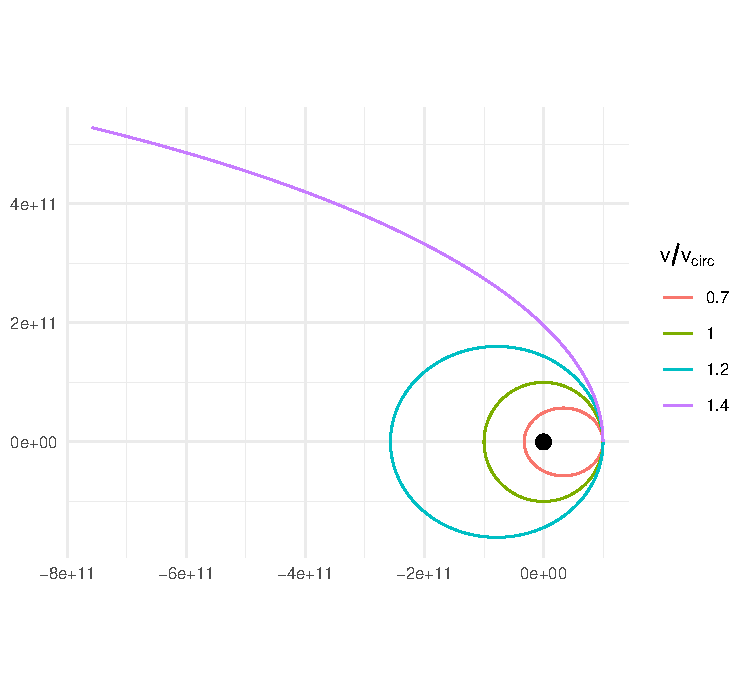
\includegraphics[width=0.8\linewidth,height=\textheight,keepaspectratio]{04-the-two-body-problem_files/figure-pdf/fig-speed-sweep-1.pdf}

}

\caption{\label{fig-speed-sweep}The same launch point, four launch
speeds. The circle is \(k = 1\); slower launches dip inward from
apoapsis, faster ones swing outward from periapsis. The \(k = 1.4\)
orbit has \(e = 0.96\) and a period of nearly a century, so two years
show only its beginning.}

\end{figure}%

\subsection{Measuring eccentricity from a single
state}\label{measuring-eccentricity-from-a-single-state}

Equation~\ref{eq-ecc-vector} is more than a derivation device. It gives
the eccentricity from the position and velocity at \emph{any one
instant}, no full orbit required. Two helpers make that easy. The first
extracts the relative motion of one body about another, the quantity all
of this chapter's formulas are about:

\begin{Shaded}
\begin{Highlighting}[]
\NormalTok{relative\_state }\OtherTok{\textless{}{-}} \ControlFlowTok{function}\NormalTok{(sim, body, center, }\AttributeTok{G =}\NormalTok{ gravitational\_constant) \{}
\NormalTok{  ctr }\OtherTok{\textless{}{-}}\NormalTok{ sim }\SpecialCharTok{|\textgreater{}}
    \FunctionTok{filter}\NormalTok{(id }\SpecialCharTok{==}\NormalTok{ center) }\SpecialCharTok{|\textgreater{}}
    \FunctionTok{select}\NormalTok{(time, }\AttributeTok{m\_c =}\NormalTok{ mass, }\AttributeTok{x\_c =}\NormalTok{ x, }\AttributeTok{y\_c =}\NormalTok{ y, }\AttributeTok{z\_c =}\NormalTok{ z,}
           \AttributeTok{vx\_c =}\NormalTok{ vx, }\AttributeTok{vy\_c =}\NormalTok{ vy, }\AttributeTok{vz\_c =}\NormalTok{ vz)}
\NormalTok{  sim }\SpecialCharTok{|\textgreater{}}
    \FunctionTok{filter}\NormalTok{(id }\SpecialCharTok{==}\NormalTok{ body) }\SpecialCharTok{|\textgreater{}}
    \FunctionTok{inner\_join}\NormalTok{(ctr, }\AttributeTok{by =} \StringTok{"time"}\NormalTok{) }\SpecialCharTok{|\textgreater{}}
    \FunctionTok{mutate}\NormalTok{(}\AttributeTok{mu =}\NormalTok{ G }\SpecialCharTok{*}\NormalTok{ (mass }\SpecialCharTok{+}\NormalTok{ m\_c),}
           \AttributeTok{rx =}\NormalTok{ x }\SpecialCharTok{{-}}\NormalTok{ x\_c,   }\AttributeTok{ry =}\NormalTok{ y }\SpecialCharTok{{-}}\NormalTok{ y\_c,   }\AttributeTok{rz =}\NormalTok{ z }\SpecialCharTok{{-}}\NormalTok{ z\_c,}
           \AttributeTok{ux =}\NormalTok{ vx }\SpecialCharTok{{-}}\NormalTok{ vx\_c, }\AttributeTok{uy =}\NormalTok{ vy }\SpecialCharTok{{-}}\NormalTok{ vy\_c, }\AttributeTok{uz =}\NormalTok{ vz }\SpecialCharTok{{-}}\NormalTok{ vz\_c) }\SpecialCharTok{|\textgreater{}}
    \FunctionTok{select}\NormalTok{(time, mu, rx, ry, rz, ux, uy, uz)}
\NormalTok{\}}
\end{Highlighting}
\end{Shaded}

The second computes \(\mathbf{h} = \mathbf{r}\times\mathbf{u}\) and then
\(\mathbf{e} = (\mathbf{u}\times\mathbf{h})/\mu - \mathbf{r}/r\)
component by component:

\begin{Shaded}
\begin{Highlighting}[]
\NormalTok{eccentricity }\OtherTok{\textless{}{-}} \ControlFlowTok{function}\NormalTok{(sim, body, center, }\AttributeTok{G =}\NormalTok{ gravitational\_constant) \{}
  \FunctionTok{relative\_state}\NormalTok{(sim, body, center, G) }\SpecialCharTok{|\textgreater{}}
    \FunctionTok{mutate}\NormalTok{(}\AttributeTok{r  =} \FunctionTok{sqrt}\NormalTok{(rx}\SpecialCharTok{\^{}}\DecValTok{2} \SpecialCharTok{+}\NormalTok{ ry}\SpecialCharTok{\^{}}\DecValTok{2} \SpecialCharTok{+}\NormalTok{ rz}\SpecialCharTok{\^{}}\DecValTok{2}\NormalTok{),}
           \AttributeTok{hx =}\NormalTok{ ry }\SpecialCharTok{*}\NormalTok{ uz }\SpecialCharTok{{-}}\NormalTok{ rz }\SpecialCharTok{*}\NormalTok{ uy,                   }\CommentTok{\# h = r x u}
           \AttributeTok{hy =}\NormalTok{ rz }\SpecialCharTok{*}\NormalTok{ ux }\SpecialCharTok{{-}}\NormalTok{ rx }\SpecialCharTok{*}\NormalTok{ uz,}
           \AttributeTok{hz =}\NormalTok{ rx }\SpecialCharTok{*}\NormalTok{ uy }\SpecialCharTok{{-}}\NormalTok{ ry }\SpecialCharTok{*}\NormalTok{ ux,}
           \AttributeTok{ex =}\NormalTok{ (uy }\SpecialCharTok{*}\NormalTok{ hz }\SpecialCharTok{{-}}\NormalTok{ uz }\SpecialCharTok{*}\NormalTok{ hy) }\SpecialCharTok{/}\NormalTok{ mu }\SpecialCharTok{{-}}\NormalTok{ rx }\SpecialCharTok{/}\NormalTok{ r,  }\CommentTok{\# e = (u x h)/mu {-} r/r}
           \AttributeTok{ey =}\NormalTok{ (uz }\SpecialCharTok{*}\NormalTok{ hx }\SpecialCharTok{{-}}\NormalTok{ ux }\SpecialCharTok{*}\NormalTok{ hz) }\SpecialCharTok{/}\NormalTok{ mu }\SpecialCharTok{{-}}\NormalTok{ ry }\SpecialCharTok{/}\NormalTok{ r,}
           \AttributeTok{ez =}\NormalTok{ (ux }\SpecialCharTok{*}\NormalTok{ hy }\SpecialCharTok{{-}}\NormalTok{ uy }\SpecialCharTok{*}\NormalTok{ hx) }\SpecialCharTok{/}\NormalTok{ mu }\SpecialCharTok{{-}}\NormalTok{ rz }\SpecialCharTok{/}\NormalTok{ r,}
           \AttributeTok{e  =} \FunctionTok{sqrt}\NormalTok{(ex}\SpecialCharTok{\^{}}\DecValTok{2} \SpecialCharTok{+}\NormalTok{ ey}\SpecialCharTok{\^{}}\DecValTok{2} \SpecialCharTok{+}\NormalTok{ ez}\SpecialCharTok{\^{}}\DecValTok{2}\NormalTok{)) }\SpecialCharTok{|\textgreater{}}
    \FunctionTok{select}\NormalTok{(time, e, ex, ey, ez)}
\NormalTok{\}}
\end{Highlighting}
\end{Shaded}

Now compare the prediction \(e = |k^2 - 1|\) with the eccentricity
measured from the simulated state at the \emph{end} of each run, two
years of integration away from the initial conditions:

\begin{Shaded}
\begin{Highlighting}[]
\NormalTok{sweep }\SpecialCharTok{|\textgreater{}}
  \FunctionTok{group\_by}\NormalTok{(k) }\SpecialCharTok{|\textgreater{}}
  \FunctionTok{group\_modify}\NormalTok{(}\SpecialCharTok{\textasciitilde{}} \FunctionTok{eccentricity}\NormalTok{(.x, }\StringTok{"Planet"}\NormalTok{, }\StringTok{"Star"}\NormalTok{) }\SpecialCharTok{|\textgreater{}}
                 \FunctionTok{filter}\NormalTok{(time }\SpecialCharTok{==} \FunctionTok{max}\NormalTok{(time))) }\SpecialCharTok{|\textgreater{}}
  \FunctionTok{ungroup}\NormalTok{() }\SpecialCharTok{|\textgreater{}}
  \FunctionTok{mutate}\NormalTok{(}\AttributeTok{predicted =} \FunctionTok{abs}\NormalTok{(k}\SpecialCharTok{\^{}}\DecValTok{2} \SpecialCharTok{{-}} \DecValTok{1}\NormalTok{)) }\SpecialCharTok{|\textgreater{}}
  \FunctionTok{select}\NormalTok{(k, predicted, }\AttributeTok{measured =}\NormalTok{ e)}
\CommentTok{\#\textgreater{} \# A tibble: 4 x 3}
\CommentTok{\#\textgreater{}       k predicted    measured}
\CommentTok{\#\textgreater{}   \textless{}dbl\textgreater{}     \textless{}dbl\textgreater{}       \textless{}dbl\textgreater{}}
\CommentTok{\#\textgreater{} 1   0.7      0.51 0.510      }
\CommentTok{\#\textgreater{} 2   1        0    0.000000413}
\CommentTok{\#\textgreater{} 3   1.2      0.44 0.440      }
\CommentTok{\#\textgreater{} 4   1.4      0.96 0.960}
\end{Highlighting}
\end{Shaded}

The agreement is to many decimal places. And since \(\mathbf{e}\) is
supposed to be a constant of the motion, we can ask how constant the
simulation kept it over the whole two years for the \(k = 1.2\) orbit:

\begin{Shaded}
\begin{Highlighting}[]
\NormalTok{e\_track }\OtherTok{\textless{}{-}} \FunctionTok{eccentricity}\NormalTok{(}\FunctionTok{filter}\NormalTok{(sweep, k }\SpecialCharTok{==} \FloatTok{1.2}\NormalTok{), }\StringTok{"Planet"}\NormalTok{, }\StringTok{"Star"}\NormalTok{)}
\FunctionTok{range}\NormalTok{(e\_track}\SpecialCharTok{$}\NormalTok{e)}
\CommentTok{\#\textgreater{} [1] 0.4400000 0.4400002}
\end{Highlighting}
\end{Shaded}

The spread between the smallest and largest value is the integrator's
error. It is small. Chapter 5 explains why it is small and what it
depends on, and shows what the same test looks like with a worse
integrator.

The package does this computation for you.
\texttt{get\_orbital\_elements()} applies exactly the
eccentricity-vector and vis-viva formulas of this chapter to every time
step and returns the full set of orbital elements, with the semi-major
axis and the Kepler's-third-law period alongside the eccentricity:

\begin{Shaded}
\begin{Highlighting}[]
\FunctionTok{get\_orbital\_elements}\NormalTok{(}\FunctionTok{filter}\NormalTok{(sweep, k }\SpecialCharTok{==} \FloatTok{1.2}\NormalTok{), }\StringTok{"Planet"}\NormalTok{, }\StringTok{"Star"}\NormalTok{,}
                     \AttributeTok{mu =}\NormalTok{ gravitational\_constant }\SpecialCharTok{*}\NormalTok{ (M }\SpecialCharTok{+}\NormalTok{ m)) }\SpecialCharTok{|\textgreater{}}
  \FunctionTok{summarise}\NormalTok{(}\AttributeTok{e =} \FunctionTok{mean}\NormalTok{(e), }\AttributeTok{a =} \FunctionTok{mean}\NormalTok{(a), }\AttributeTok{period\_days =} \FunctionTok{mean}\NormalTok{(period) }\SpecialCharTok{/}\NormalTok{ seconds\_per\_day)}
\CommentTok{\#\textgreater{} \# A tibble: 1 x 3}
\CommentTok{\#\textgreater{}       e             a period\_days}
\CommentTok{\#\textgreater{}   \textless{}dbl\textgreater{}         \textless{}dbl\textgreater{}       \textless{}dbl\textgreater{}}
\CommentTok{\#\textgreater{} 1 0.440 178571465973.        672.}
\end{Highlighting}
\end{Shaded}

(The \texttt{mu} argument is there because, by default, the function
uses the parent's mass alone, which is the convention of
\texttt{add\_body\_keplerian()} and is exact in the test-particle limit;
passing \(G(M+m)\) gives the exact two-body elements, which is what the
derivations here are about.) I wrote \texttt{eccentricity()} out by hand
above so that you could see the formula do its work; from here on the
book uses the package function, and Chapter 7 derives the rest of what
it computes.

\subsection{Measuring the period}\label{measuring-the-period}

Kepler's third law needs a period. \texttt{get\_orbital\_elements()}
reports one, but it is computed \emph{from} the third law,
\(T = 2\pi\sqrt{a^3/\mu}\), so using it to check the third law would be
circular. An independent measurement means finding when the body has
actually gone all the way round. The cleanest way is to track the polar
angle of the relative position, unwrap the jump from \(+\pi\) to
\(-\pi\), and interpolate to the moment the total angle reaches
\(2\pi\):

\begin{Shaded}
\begin{Highlighting}[]
\NormalTok{measure\_period }\OtherTok{\textless{}{-}} \ControlFlowTok{function}\NormalTok{(sim, body, }\AttributeTok{center =} \ConstantTok{NULL}\NormalTok{, }\AttributeTok{G =}\NormalTok{ gravitational\_constant) \{}
  \ControlFlowTok{if}\NormalTok{ (}\FunctionTok{is.null}\NormalTok{(center)) \{                              }\CommentTok{\# measure about the origin}
\NormalTok{    rel }\OtherTok{\textless{}{-}}\NormalTok{ sim }\SpecialCharTok{|\textgreater{}} \FunctionTok{filter}\NormalTok{(id }\SpecialCharTok{==}\NormalTok{ body) }\SpecialCharTok{|\textgreater{}} \FunctionTok{transmute}\NormalTok{(time, }\AttributeTok{rx =}\NormalTok{ x, }\AttributeTok{ry =}\NormalTok{ y)}
\NormalTok{  \} }\ControlFlowTok{else}\NormalTok{ \{}
\NormalTok{    rel }\OtherTok{\textless{}{-}} \FunctionTok{relative\_state}\NormalTok{(sim, body, center, G)}
\NormalTok{  \}}
\NormalTok{  theta  }\OtherTok{\textless{}{-}} \FunctionTok{atan2}\NormalTok{(rel}\SpecialCharTok{$}\NormalTok{ry, rel}\SpecialCharTok{$}\NormalTok{rx)}
\NormalTok{  dtheta }\OtherTok{\textless{}{-}}\NormalTok{ ((}\FunctionTok{diff}\NormalTok{(theta) }\SpecialCharTok{+}\NormalTok{ pi) }\SpecialCharTok{\%\%}\NormalTok{ (}\DecValTok{2} \SpecialCharTok{*}\NormalTok{ pi)) }\SpecialCharTok{{-}}\NormalTok{ pi   }\CommentTok{\# unwrap the jump at +/{-} pi}
\NormalTok{  swept  }\OtherTok{\textless{}{-}} \FunctionTok{abs}\NormalTok{(}\FunctionTok{cumsum}\NormalTok{(}\FunctionTok{c}\NormalTok{(}\DecValTok{0}\NormalTok{, dtheta)))                }\CommentTok{\# total angle travelled}
\NormalTok{  i }\OtherTok{\textless{}{-}} \FunctionTok{which}\NormalTok{(swept }\SpecialCharTok{\textgreater{}=} \DecValTok{2} \SpecialCharTok{*}\NormalTok{ pi)[}\DecValTok{1}\NormalTok{]}
  \ControlFlowTok{if}\NormalTok{ (}\FunctionTok{is.na}\NormalTok{(i)) }\FunctionTok{return}\NormalTok{(}\ConstantTok{NA\_real\_}\NormalTok{)                     }\CommentTok{\# the run was too short}
\NormalTok{  f }\OtherTok{\textless{}{-}}\NormalTok{ (}\DecValTok{2} \SpecialCharTok{*}\NormalTok{ pi }\SpecialCharTok{{-}}\NormalTok{ swept[i }\SpecialCharTok{{-}} \DecValTok{1}\NormalTok{]) }\SpecialCharTok{/}\NormalTok{ (swept[i] }\SpecialCharTok{{-}}\NormalTok{ swept[i }\SpecialCharTok{{-}} \DecValTok{1}\NormalTok{])}
\NormalTok{  rel}\SpecialCharTok{$}\NormalTok{time[i }\SpecialCharTok{{-}} \DecValTok{1}\NormalTok{] }\SpecialCharTok{+}\NormalTok{ f }\SpecialCharTok{*}\NormalTok{ (rel}\SpecialCharTok{$}\NormalTok{time[i] }\SpecialCharTok{{-}}\NormalTok{ rel}\SpecialCharTok{$}\NormalTok{time[i }\SpecialCharTok{{-}} \DecValTok{1}\NormalTok{])}
\NormalTok{\}}
\end{Highlighting}
\end{Shaded}

For the circular case, Equation~\ref{eq-kepler3} with \(a = r_0\):

\begin{Shaded}
\begin{Highlighting}[]
\NormalTok{T\_pred }\OtherTok{\textless{}{-}} \DecValTok{2} \SpecialCharTok{*}\NormalTok{ pi }\SpecialCharTok{*} \FunctionTok{sqrt}\NormalTok{(r0}\SpecialCharTok{\^{}}\DecValTok{3} \SpecialCharTok{/}\NormalTok{ mu)}
\NormalTok{T\_meas }\OtherTok{\textless{}{-}} \FunctionTok{measure\_period}\NormalTok{(}\FunctionTok{filter}\NormalTok{(sweep, k }\SpecialCharTok{==} \DecValTok{1}\NormalTok{), }\StringTok{"Planet"}\NormalTok{, }\StringTok{"Star"}\NormalTok{)}

\FunctionTok{c}\NormalTok{(}\AttributeTok{predicted\_days =}\NormalTok{ T\_pred }\SpecialCharTok{/}\NormalTok{ seconds\_per\_day,}
  \AttributeTok{measured\_days  =}\NormalTok{ T\_meas }\SpecialCharTok{/}\NormalTok{ seconds\_per\_day)}
\CommentTok{\#\textgreater{} predicted\_days  measured\_days }
\CommentTok{\#\textgreater{}       281.4900       281.4901}
\end{Highlighting}
\end{Shaded}

For the \(k = 1.2\) ellipse the semi-major axis is \(a = r_p/(1-e)\)
with \(r_p = r_0\) and \(e = 0.44\), which makes the orbit larger and
the period longer:

\begin{Shaded}
\begin{Highlighting}[]
\NormalTok{a\_12   }\OtherTok{\textless{}{-}}\NormalTok{ r0 }\SpecialCharTok{/}\NormalTok{ (}\DecValTok{1} \SpecialCharTok{{-}} \FloatTok{0.44}\NormalTok{)}
\NormalTok{T\_pred }\OtherTok{\textless{}{-}} \DecValTok{2} \SpecialCharTok{*}\NormalTok{ pi }\SpecialCharTok{*} \FunctionTok{sqrt}\NormalTok{(a\_12}\SpecialCharTok{\^{}}\DecValTok{3} \SpecialCharTok{/}\NormalTok{ mu)}
\NormalTok{T\_meas }\OtherTok{\textless{}{-}} \FunctionTok{measure\_period}\NormalTok{(}\FunctionTok{filter}\NormalTok{(sweep, k }\SpecialCharTok{==} \FloatTok{1.2}\NormalTok{), }\StringTok{"Planet"}\NormalTok{, }\StringTok{"Star"}\NormalTok{)}

\FunctionTok{c}\NormalTok{(}\AttributeTok{predicted\_days =}\NormalTok{ T\_pred }\SpecialCharTok{/}\NormalTok{ seconds\_per\_day,}
  \AttributeTok{measured\_days  =}\NormalTok{ T\_meas }\SpecialCharTok{/}\NormalTok{ seconds\_per\_day)}
\CommentTok{\#\textgreater{} predicted\_days  measured\_days }
\CommentTok{\#\textgreater{}       671.7088       671.7090}
\end{Highlighting}
\end{Shaded}

\subsection{The Moon, revisited}\label{the-moon-revisited}

Chapter 2's four-line Moon started at the semi-major-axis distance of
384,400 km with the mean orbital speed of 1,022 m/s. We can now say
exactly what orbit that is. The circular speed at that distance, with
the full \(\mu = G(M_{\mathrm{Earth}} + m_{\mathrm{Moon}})\), is a
little \emph{higher} than 1,022 m/s, so the launch point is apoapsis and
the orbit dips inward:

\begin{Shaded}
\begin{Highlighting}[]
\NormalTok{mu\_em  }\OtherTok{\textless{}{-}}\NormalTok{ gravitational\_constant }\SpecialCharTok{*}\NormalTok{ (mass\_earth }\SpecialCharTok{+}\NormalTok{ mass\_moon)}
\NormalTok{k\_moon }\OtherTok{\textless{}{-}}\NormalTok{ speed\_moon }\SpecialCharTok{/} \FunctionTok{sqrt}\NormalTok{(mu\_em }\SpecialCharTok{/}\NormalTok{ distance\_earth\_moon)}
\NormalTok{e\_moon }\OtherTok{\textless{}{-}} \FunctionTok{abs}\NormalTok{(k\_moon}\SpecialCharTok{\^{}}\DecValTok{2} \SpecialCharTok{{-}} \DecValTok{1}\NormalTok{)}
\NormalTok{a\_moon }\OtherTok{\textless{}{-}}\NormalTok{ distance\_earth\_moon }\SpecialCharTok{/}\NormalTok{ (}\DecValTok{1} \SpecialCharTok{+}\NormalTok{ e\_moon)      }\CommentTok{\# launch point is apoapsis}
\NormalTok{T\_moon }\OtherTok{\textless{}{-}} \DecValTok{2} \SpecialCharTok{*}\NormalTok{ pi }\SpecialCharTok{*} \FunctionTok{sqrt}\NormalTok{(a\_moon}\SpecialCharTok{\^{}}\DecValTok{3} \SpecialCharTok{/}\NormalTok{ mu\_em)}

\FunctionTok{c}\NormalTok{(}\AttributeTok{k =}\NormalTok{ k\_moon, }\AttributeTok{e =}\NormalTok{ e\_moon, }\AttributeTok{a\_km =}\NormalTok{ a\_moon }\SpecialCharTok{/} \FloatTok{1e3}\NormalTok{, }\AttributeTok{T\_days =}\NormalTok{ T\_moon }\SpecialCharTok{/}\NormalTok{ seconds\_per\_day)}
\CommentTok{\#\textgreater{}            k            e         a\_km       T\_days }
\CommentTok{\#\textgreater{} 9.975312e{-}01 4.931523e{-}03 3.825136e+05 2.708447e+01}
\end{Highlighting}
\end{Shaded}

Against the simulation:

\begin{Shaded}
\begin{Highlighting}[]
\NormalTok{moon }\OtherTok{\textless{}{-}} \FunctionTok{create\_system}\NormalTok{() }\SpecialCharTok{|\textgreater{}}
  \FunctionTok{add\_body}\NormalTok{(}\StringTok{"Earth"}\NormalTok{, }\AttributeTok{mass =}\NormalTok{ mass\_earth) }\SpecialCharTok{|\textgreater{}}
  \FunctionTok{add\_body}\NormalTok{(}\StringTok{"Moon"}\NormalTok{,  }\AttributeTok{mass =}\NormalTok{ mass\_moon, }\AttributeTok{x =}\NormalTok{ distance\_earth\_moon, }\AttributeTok{vy =}\NormalTok{ speed\_moon) }\SpecialCharTok{|\textgreater{}}
  \FunctionTok{simulate\_system}\NormalTok{(}\AttributeTok{time\_step =}\NormalTok{ seconds\_per\_hour, }\AttributeTok{duration =}\NormalTok{ seconds\_per\_day }\SpecialCharTok{*} \DecValTok{28}\NormalTok{)}

\FunctionTok{measure\_period}\NormalTok{(moon, }\StringTok{"Moon"}\NormalTok{, }\StringTok{"Earth"}\NormalTok{) }\SpecialCharTok{/}\NormalTok{ seconds\_per\_day}
\CommentTok{\#\textgreater{} [1] 27.08531}
\end{Highlighting}
\end{Shaded}

The simulation and the formula agree. But the real Moon's sidereal
period is 27.32 days, and the four-line Moon's is about 27.1. The
simulation is not wrong; the \emph{setup} describes a slightly different
orbit from the real one. ``Semi-major axis'' and ``mean speed'' are two
properties of the real elliptical orbit, but using one as a starting
distance and the other as a starting speed does not reproduce that
ellipse; it produces a nearby one with a smaller \(a\) and hence a
shorter period. The right way to put a body on its real orbit is to
specify the orbit itself, by its orbital elements, and let the package
compute a consistent position and velocity. That is what
\texttt{add\_planet()} does and what Chapter 7 derives.

\begin{tcolorbox}[enhanced jigsaw, arc=.35mm, bottomrule=.15mm, bottomtitle=1mm, breakable, colback=white, colbacktitle=quarto-callout-tip-color!10!white, colframe=quarto-callout-tip-color-frame, coltitle=black, left=2mm, leftrule=.75mm, opacityback=0, opacitybacktitle=0.6, rightrule=.15mm, title={Key results}, titlerule=0mm, toprule=.15mm, toptitle=1mm]

For the relative motion of two bodies with \(\mu = G(m_1 + m_2)\):

\begin{itemize}
\tightlist
\item
  \(\mathbf{h} = \mathbf{r}\times\dot{\mathbf{r}}\) and
  \(\varepsilon = v^2/2 - \mu/r\) are constant; the orbit is planar and
  sweeps equal areas in equal times.
\item
  Orbit equation: \(r = a(1-e^2)/(1+e\cos\nu)\), with the central body
  at a focus. \(e<1\) bound, \(e \ge 1\) unbound.
\item
  \(\varepsilon = -\mu/2a\), independent of \(e\).
\item
  Vis-viva: \(v^2 = \mu(2/r - 1/a)\). Circular speed \(\sqrt{\mu/r}\);
  escape speed \(\sqrt{2\mu/r}\).
\item
  Launching perpendicular to the radius at \(k\) times circular speed
  gives \(e = |k^2-1|\).
\item
  Period: \(T = 2\pi\sqrt{a^3/\mu}\).
\item
  \(e = (r_a - r_p)/(r_a + r_p)\), and
  \(\mathbf{e} = (\dot{\mathbf{r}}\times\mathbf{h})/\mu - \mathbf{r}/r\)
  from any single state.
\end{itemize}

\end{tcolorbox}

\chapter{Integrators: Euler, Euler-Cromer, and Velocity
Verlet}\label{sec-integrators}

Chapter 3 ended with the two halves of every N-body code: a function
that computes accelerations from positions, and a function that advances
the state by one step. This chapter is about the second one.
\texttt{simulate\_system()} offers three choices for it, through its
\texttt{method} argument: \texttt{"euler"}, \texttt{"euler\_cromer"},
and \texttt{"verlet"}, the default. They differ by a few characters of
code and by everything that matters. The textbook method quietly feeds
energy into every orbit it touches; the default keeps a planet on a
closed ellipse for as long as you care to run it. The reason is not that
Verlet is ``more accurate'' in the usual sense. It is that Verlet
respects a geometric property of Newton's equations that Euler violates,
and the goal of this chapter is to make that property concrete enough
that you could check for it yourself.

\section{The problem of taking a
step}\label{the-problem-of-taking-a-step}

The state of a body is its position \(\mathbf{x}\) and velocity
\(\mathbf{v}\), and the equations of motion say
\(\dot{\mathbf{x}} = \mathbf{v}\) and
\(\dot{\mathbf{v}} = \mathbf{a}(\mathbf{x})\), where the acceleration
depends only on positions (Chapter 3). Given the state at time \(t\), we
want the state at \(t + \Delta t\).

Taylor's theorem is the whole toolkit. For a smooth trajectory,

\begin{equation}\protect\phantomsection\label{eq-taylor}{
\begin{aligned}
\mathbf{x}(t+\Delta t) &= \mathbf{x} + \mathbf{v}\,\Delta t + \tfrac12\,\mathbf{a}\,\Delta t^2 + \tfrac16\,\dot{\mathbf{a}}\,\Delta t^3 + O(\Delta t^4), \\
\mathbf{v}(t+\Delta t) &= \mathbf{v} + \mathbf{a}\,\Delta t + \tfrac12\,\dot{\mathbf{a}}\,\Delta t^2 + O(\Delta t^3),
\end{aligned}
}\end{equation}

where everything on the right is evaluated at \(t\). We know
\(\mathbf{x}\) and \(\mathbf{v}\), and we can compute \(\mathbf{a}\)
from \(\mathbf{x}\). We do not know \(\dot{\mathbf{a}}\) or anything
beyond it. Every integrator is a decision about what to do with the
terms we cannot compute.

A method whose single-step error is \(O(\Delta t^{p+1})\) is said to be
of \emph{order} \(p\), because over a fixed total time \(T\) there are
\(T/\Delta t\) steps and the errors accumulate to \(O(\Delta t^p)\).
Halve the step and a first-order method's error halves; a second-order
method's error drops by four. That is the usual way to grade
integrators, and it will turn out to be only half the story.

\section{Euler's method}\label{eulers-method}

The simplest decision is to keep only the terms we can compute exactly
and drop the rest:

\begin{equation}\protect\phantomsection\label{eq-euler}{
\begin{aligned}
\mathbf{x}_{n+1} &= \mathbf{x}_n + \mathbf{v}_n\,\Delta t, \\
\mathbf{v}_{n+1} &= \mathbf{v}_n + \mathbf{a}_n\,\Delta t.
\end{aligned}
}\end{equation}

Both updates truncate Equation~\ref{eq-taylor} after the first power of
\(\Delta t\), so the local error is \(O(\Delta t^2)\) and the method is
first order. It is what every introductory text starts with, and it is
\texttt{method\ =\ "euler"}.

It is also wrong for orbits in a way that halving the step does not fix.
Consider a body on a circular orbit, where
\(\mathbf{v} \perp \mathbf{x}\) and \(\mathbf{a} \perp \mathbf{v}\).
After one Euler step,

\[
|\mathbf{x}_{n+1}|^2 = |\mathbf{x}_n|^2 + 2\Delta t\,\mathbf{x}_n\cdot\mathbf{v}_n + \Delta t^2 |\mathbf{v}_n|^2 = r^2 + v^2\Delta t^2,
\]

so the body ends the step slightly farther out, and

\[
|\mathbf{v}_{n+1}|^2 = v^2 + 2\Delta t\,\mathbf{v}_n\cdot\mathbf{a}_n + \Delta t^2 a^2 = v^2 + a^2\Delta t^2,
\]

so it also ends the step slightly faster. Farther out means higher
potential energy; faster means higher kinetic energy. Every single step
adds energy to the orbit, in both accounts at once, and there is no step
that ever takes any back. The orbit spirals outward, forever. A smaller
\(\Delta t\) makes each step's contribution smaller, but there are
correspondingly more steps, and the sign never changes.

There is a cleaner way to see what is going on, using the simplest
oscillating system there is: a mass on a spring,
\(\ddot{x} = -\omega^2 x\), with state \((x, v)\). One Euler step is a
linear map,

\begin{equation}\protect\phantomsection\label{eq-euler-matrix}{
\begin{pmatrix} x_{n+1} \\ v_{n+1} \end{pmatrix}
= \underbrace{\begin{pmatrix} 1 & \Delta t \\ -\omega^2\Delta t & 1 \end{pmatrix}}_{M_{\mathrm{E}}}
\begin{pmatrix} x_n \\ v_n \end{pmatrix},
\qquad \det M_{\mathrm{E}} = 1 + \omega^2\Delta t^2.
}\end{equation}

The determinant of a linear map is the factor by which it scales areas.
The true dynamics of the oscillator carries any region of the \((x, v)\)
plane around an ellipse without changing its area, a fact that holds for
every Hamiltonian system and is known as Liouville's theorem. Euler's
map scales area by \(1 + \omega^2\Delta t^2 > 1\) on every step. The
oscillator's energy is proportional to the area of the ellipse it traces
in the \((x, v)\) plane, so a map that inflates areas inflates energies.
Nothing about that depends on \(\Delta t\) being large.

\section{Euler-Cromer}\label{euler-cromer}

Here is a change so small it looks like a typo:

\begin{equation}\protect\phantomsection\label{eq-euler-cromer}{
\begin{aligned}
\mathbf{v}_{n+1} &= \mathbf{v}_n + \mathbf{a}_n\,\Delta t, \\
\mathbf{x}_{n+1} &= \mathbf{x}_n + \mathbf{v}_{n+1}\,\Delta t.
\end{aligned}
}\end{equation}

The velocity is updated first, and the position update uses the
\emph{new} velocity. This is \texttt{method\ =\ "euler\_cromer"}, also
called the semi-implicit Euler method or symplectic Euler. Its local
error is still \(O(\Delta t^2)\): it is a first-order method, no more
accurate than plain Euler by the usual grading. But redo the oscillator
calculation. Substituting the first line into the second,
\(x_{n+1} = x_n + (v_n - \omega^2 x_n \Delta t)\Delta t\), so

\begin{equation}\protect\phantomsection\label{eq-ec-matrix}{
M_{\mathrm{EC}} = \begin{pmatrix} 1 - \omega^2\Delta t^2 & \Delta t \\ -\omega^2\Delta t & 1 \end{pmatrix},
\qquad \det M_{\mathrm{EC}} = (1 - \omega^2\Delta t^2) + \omega^2\Delta t^2 = 1.
}\end{equation}

Exactly one. The Euler-Cromer map preserves area, for every
\(\Delta t\), just as the true dynamics does. An integrator with this
property is called \emph{symplectic}. (In one spatial dimension,
symplectic means area-preserving; in more dimensions it is a slightly
stronger condition that reduces to the same idea.) A symplectic
integrator cannot have the systematic energy drift that Euler has,
because energy drift is area growth. Its energy error oscillates, and
for a small enough step it stays bounded forever.

\begin{tcolorbox}[enhanced jigsaw, arc=.35mm, bottomrule=.15mm, bottomtitle=1mm, breakable, colback=white, colbacktitle=quarto-callout-note-color!10!white, colframe=quarto-callout-note-color-frame, coltitle=black, left=2mm, leftrule=.75mm, opacityback=0, opacitybacktitle=0.6, rightrule=.15mm, title={Where it comes from}, titlerule=0mm, toprule=.15mm, toptitle=1mm]

The method is named for Alan Cromer, who published it in a two-page note
in the \emph{American Journal of Physics} in 1981 (Cromer 1981). He
reports that the reordering was found by one of his students, who
noticed that it made the Euler method work on oscillators when it
otherwise would not. The method itself had been known to numerical
analysts under other names, but Cromer's note is where the
physics-teaching community learned that the order of two lines of code
could be the difference between a stable orbit and an unstable one.

\end{tcolorbox}

Why does this version work when the other does not? The position update
in Equation~\ref{eq-euler-cromer} uses \(\mathbf{v}_{n+1}\), which is
the velocity at the \emph{end} of the step. In effect it averages a
forward-looking velocity with a backward-looking acceleration, and the
two mistakes cancel in exactly the way needed to preserve area. There is
a deeper structure here: the map is the composition of two exact flows,
a ``kick'' that changes only the velocity and a ``drift'' that changes
only the position, and each of those is itself symplectic because it is
the exact solution of a Hamiltonian system (a free particle for the
drift, a particle frozen in place for the kick). Composing symplectic
maps gives a symplectic map. Plain Euler is not a composition of exact
flows, and that is what it costs.

Euler-Cromer is fast, needing one acceleration evaluation per step, and
is a reasonable choice for a quick preview. But first order is first
order. Its positions drift in \emph{phase} along the orbit at a rate
proportional to \(\Delta t\) even when the energy is right, so a planet
simulated with Euler-Cromer is on the correct ellipse at the wrong time.
Something better is needed for real work.

\section{Velocity Verlet}\label{velocity-verlet}

Go back to Equation~\ref{eq-taylor} and keep one more term. The position
expansion through \(\Delta t^2\) uses only quantities we have,

\[
\mathbf{x}_{n+1} = \mathbf{x}_n + \mathbf{v}_n\Delta t + \tfrac12\mathbf{a}_n\Delta t^2,
\]

with local error \(O(\Delta t^3)\). For the velocity, the troublesome
term is \(\tfrac12\dot{\mathbf{a}}\Delta t^2\). We cannot compute
\(\dot{\mathbf{a}}\) directly, but having just computed
\(\mathbf{x}_{n+1}\), we can compute
\(\mathbf{a}_{n+1} = \mathbf{a}(\mathbf{x}_{n+1})\), and then
approximate the derivative by the difference quotient
\(\dot{\mathbf{a}} \approx (\mathbf{a}_{n+1} - \mathbf{a}_n)/\Delta t\).
Substituting,

\[
\mathbf{v}_{n+1} = \mathbf{v}_n + \mathbf{a}_n\Delta t + \tfrac12(\mathbf{a}_{n+1} - \mathbf{a}_n)\Delta t
= \mathbf{v}_n + \tfrac12(\mathbf{a}_n + \mathbf{a}_{n+1})\Delta t.
\]

Together:

\begin{equation}\protect\phantomsection\label{eq-verlet}{
\begin{aligned}
\mathbf{x}_{n+1} &= \mathbf{x}_n + \mathbf{v}_n\,\Delta t + \tfrac12\,\mathbf{a}_n\,\Delta t^2, \\
\mathbf{a}_{n+1} &= \mathbf{a}(\mathbf{x}_{n+1}), \\
\mathbf{v}_{n+1} &= \mathbf{v}_n + \tfrac12\left(\mathbf{a}_n + \mathbf{a}_{n+1}\right)\Delta t.
\end{aligned}
}\end{equation}

This is \textbf{Velocity Verlet}, \texttt{method\ =\ "verlet"}. Position
first, then the new acceleration, then the velocity using the average of
the old and new accelerations, which is exactly the recipe in the
package documentation. It is second order: halving the step divides the
error by four.

Second order is nice, but it is not why the method is the default. Redo
the oscillator one more time. With \(\mathbf{a} = -\omega^2 x\), the
position update is
\(x_{n+1} = (1 - \tfrac12\omega^2\Delta t^2)\,x_n + \Delta t\, v_n\),
and substituting into the velocity update gives, after a few lines of
algebra,

\begin{equation}\protect\phantomsection\label{eq-vv-matrix}{
M_{\mathrm{VV}} = \begin{pmatrix}
1 - \tfrac12\omega^2\Delta t^2 & \Delta t \\[2pt]
-\omega^2\Delta t\left(1 - \tfrac14\omega^2\Delta t^2\right) & 1 - \tfrac12\omega^2\Delta t^2
\end{pmatrix},
\qquad \det M_{\mathrm{VV}} = 1.
}\end{equation}

(Multiply out the determinant: the \(\omega^2\Delta t^2\) and
\(\omega^4\Delta t^4\) terms cancel exactly.) Velocity Verlet is
symplectic. It is also \emph{time-reversible}: if you take a step
forward and then a step backward with the velocity reversed, you land
exactly where you started, which is a symmetry the true equations of
motion have and Euler and Euler-Cromer do not. Symplectic,
time-reversible, and second order, at the cost of a second acceleration
evaluation per step. (orbitr computes \(\mathbf{a}_n\) at the top of
each step and \(\mathbf{a}_{n+1}\) after the position update, so a
Verlet step costs two force evaluations to Euler-Cromer's one. Since
\(\mathbf{a}_{n+1}\) is the next step's \(\mathbf{a}_n\), an
implementation that kept it would pay for only one; Chapter 15 comes
back to this.) For gravitational dynamics, that combination is very hard
to beat.

\subsection{Three names for one
method}\label{three-names-for-one-method}

Velocity Verlet has two other common forms, and recognizing them will
save you confusion when reading other codes.

\textbf{The Størmer, or position, form.} Write the Taylor expansion of
\(\mathbf{x}\) both forward and backward in time and add them. The odd
powers of \(\Delta t\) cancel:

\[
\mathbf{x}(t+\Delta t) + \mathbf{x}(t-\Delta t) = 2\mathbf{x}(t) + \mathbf{a}(t)\Delta t^2 + O(\Delta t^4),
\]

so

\begin{equation}\protect\phantomsection\label{eq-stormer}{
\mathbf{x}_{n+1} = 2\mathbf{x}_n - \mathbf{x}_{n-1} + \mathbf{a}_n\Delta t^2.
}\end{equation}

No velocities appear at all, and the local error in position is
\(O(\Delta t^4)\), one order better than the derivation of
Equation~\ref{eq-verlet} suggested. Subtracting consecutive position
updates of Equation~\ref{eq-verlet} and using the velocity update to
eliminate \(\mathbf{v}\) (a few lines of algebra worth doing once) shows
that velocity Verlet produces exactly the same sequence of positions as
Equation~\ref{eq-stormer}. Velocity Verlet is just the Störmer form with
the velocity carried along explicitly, which is convenient because you
usually want the velocity.

\textbf{The leapfrog, or kick-drift-kick, form.} Split the velocity
update of Equation~\ref{eq-verlet} in half, doing the first half before
the position update and the second half after:

\begin{equation}\protect\phantomsection\label{eq-leapfrog}{
\mathbf{v}_{n+\frac12} = \mathbf{v}_n + \tfrac12\mathbf{a}_n\Delta t, \qquad
\mathbf{x}_{n+1} = \mathbf{x}_n + \mathbf{v}_{n+\frac12}\Delta t, \qquad
\mathbf{v}_{n+1} = \mathbf{v}_{n+\frac12} + \tfrac12\mathbf{a}_{n+1}\Delta t.
}\end{equation}

Substitute the first line into the second and you recover the position
update of Equation~\ref{eq-verlet}; substitute it into the third and you
recover the velocity update. The three forms are algebraically
identical. The leapfrog form makes the kick-drift-kick structure
explicit, and like Euler-Cromer it is a composition of exact flows,
which is the structural reason it is symplectic. Astrophysicists usually
say ``leapfrog''; chemists say ``velocity Verlet''; numerical analysts
say ``Störmer-Verlet.'' They are all talking about
Equation~\ref{eq-verlet}.

\begin{tcolorbox}[enhanced jigsaw, arc=.35mm, bottomrule=.15mm, bottomtitle=1mm, breakable, colback=white, colbacktitle=quarto-callout-note-color!10!white, colframe=quarto-callout-note-color-frame, coltitle=black, left=2mm, leftrule=.75mm, opacityback=0, opacitybacktitle=0.6, rightrule=.15mm, title={Where it comes from}, titlerule=0mm, toprule=.15mm, toptitle=1mm]

The method has been discovered at least four times, by people working on
completely different problems.

The first was Newton. Proposition 1 of Book I of the \emph{Principia}
(Newton 1687) proves Kepler's area law by imagining the central force
acting as a sequence of discrete impulses: the body drifts in a straight
line, receives a kick toward the center, drifts again. Newton then lets
the interval between kicks go to zero. But stop before the limit and
what you have is the leapfrog scheme, exactly. Hairer, Lubich, and
Wanner make this point in their survey of the method (Hairer et al.
2003), and it is a satisfying one: the very first proof about orbits
under gravity was, in effect, a symplectic integrator.

The second was Carl Størmer, a Norwegian mathematician who in 1907
wanted to understand the aurora (Størmer 1907). He computed the paths of
charged particles in Earth's magnetic field, by hand, with a team of
assistants, using the position form Equation~\ref{eq-stormer}. The name
``Størmer's method'' (usually spelled Störmer in the numerical-analysis
literature) stuck.

The third was Loup Verlet, in 1967 (Verlet 1967), simulating liquid
argon as a few hundred Lennard-Jones atoms, one of the first molecular
dynamics simulations. He needed a method that would keep the total
energy of the fluid constant over long runs, found the position form,
and the chemistry community has called it the Verlet algorithm ever
since. The velocity form Equation~\ref{eq-verlet} was written down by
Swope, Andersen, Berens, and Wilson in 1982 (Swope et al. 1982), in a
paper about water clusters.

Somewhere in between, Richard Feynman taught the method to Caltech
freshmen. Chapter 9 of the first volume of the \emph{Lectures on
Physics} (Feynman et al. 1963) integrates a planetary orbit by hand,
step by step, with the velocities evaluated at the half-steps, which is
the leapfrog form. He does not give it a name.

The reason the same method keeps turning up is the reason it is orbitr's
default: anyone who needs long-time stability in a conservative system,
and tries the obvious thing first, ends up here.

\end{tcolorbox}

\subsection{What ``conserves energy'' really
means}\label{what-conserves-energy-really-means}

Velocity Verlet does \emph{not} conserve energy exactly. No method with
a fixed step can, for a nonlinear force. What it does is better than it
sounds. A symplectic integrator applied to a Hamiltonian \(H\) turns out
to be the \emph{exact} solution of a slightly different Hamiltonian,
\(\tilde H = H + \Delta t^2 H_2 + \Delta t^4 H_4 + \cdots\), called the
modified or shadow Hamiltonian. The integrator conserves \(\tilde H\)
exactly, step after step (more precisely, over exponentially long
times), so the true energy \(H\) can only wander as far from its
starting value as \(\tilde H\) differs from \(H\), which is
\(O(\Delta t^2)\). The energy error oscillates within a band and never
leaves it. This is called backward error analysis, and Hairer, Lubich,
and Wanner's book is the standard reference (Hairer et al. 2006).

Euler has no shadow Hamiltonian, because it is not symplectic, and so
its energy error is free to grow without bound. The difference between a
bounded oscillation and a secular drift is the difference between a
planet that is still there after a million years and one that is not.

\section{Seeing it in orbitr}\label{seeing-it-in-orbitr}

Here is the vignette's comparison. A star and a planet, launched at 30
km/s from \(10^{11}\) m, which is an ellipse with \(e \approx 0.35\) and
a period of about 535 days. To make the differences obvious I use a time
step of six hours rather than the vignette's one hour; with hourly steps
the same things happen, more slowly.

\begin{Shaded}
\begin{Highlighting}[]
\NormalTok{star\_planet }\OtherTok{\textless{}{-}} \FunctionTok{create\_system}\NormalTok{() }\SpecialCharTok{|\textgreater{}}
  \FunctionTok{add\_body}\NormalTok{(}\StringTok{"Star"}\NormalTok{,   }\AttributeTok{mass =} \FloatTok{1e30}\NormalTok{) }\SpecialCharTok{|\textgreater{}}
  \FunctionTok{add\_body}\NormalTok{(}\StringTok{"Planet"}\NormalTok{, }\AttributeTok{mass =} \FloatTok{1e24}\NormalTok{, }\AttributeTok{x =} \FloatTok{1e11}\NormalTok{, }\AttributeTok{vy =} \DecValTok{30000}\NormalTok{)}

\NormalTok{run }\OtherTok{\textless{}{-}} \ControlFlowTok{function}\NormalTok{(method, }\AttributeTok{time\_step =}\NormalTok{ seconds\_per\_hour }\SpecialCharTok{*} \DecValTok{6}\NormalTok{,}
                \AttributeTok{duration =}\NormalTok{ seconds\_per\_year }\SpecialCharTok{*} \DecValTok{10}\NormalTok{) \{}
\NormalTok{  star\_planet }\SpecialCharTok{|\textgreater{}}
    \FunctionTok{simulate\_system}\NormalTok{(}\AttributeTok{time\_step =}\NormalTok{ time\_step, }\AttributeTok{duration =}\NormalTok{ duration,}
                    \AttributeTok{method =}\NormalTok{ method) }\SpecialCharTok{|\textgreater{}}
    \FunctionTok{mutate}\NormalTok{(}\AttributeTok{method =}\NormalTok{ method)}
\NormalTok{\}}

\NormalTok{runs }\OtherTok{\textless{}{-}} \FunctionTok{bind\_rows}\NormalTok{(}\FunctionTok{run}\NormalTok{(}\StringTok{"verlet"}\NormalTok{), }\FunctionTok{run}\NormalTok{(}\StringTok{"euler\_cromer"}\NormalTok{), }\FunctionTok{run}\NormalTok{(}\StringTok{"euler"}\NormalTok{))}
\end{Highlighting}
\end{Shaded}

\begin{Shaded}
\begin{Highlighting}[]
\NormalTok{runs }\SpecialCharTok{|\textgreater{}}
  \FunctionTok{filter}\NormalTok{(id }\SpecialCharTok{==} \StringTok{"Planet"}\NormalTok{) }\SpecialCharTok{|\textgreater{}}
  \FunctionTok{ggplot}\NormalTok{(}\FunctionTok{aes}\NormalTok{(x, y, }\AttributeTok{color =}\NormalTok{ method)) }\SpecialCharTok{+}
  \FunctionTok{geom\_path}\NormalTok{(}\AttributeTok{alpha =} \FloatTok{0.7}\NormalTok{) }\SpecialCharTok{+}
  \FunctionTok{annotate}\NormalTok{(}\StringTok{"point"}\NormalTok{, }\AttributeTok{x =} \DecValTok{0}\NormalTok{, }\AttributeTok{y =} \DecValTok{0}\NormalTok{, }\AttributeTok{size =} \DecValTok{3}\NormalTok{) }\SpecialCharTok{+}
  \FunctionTok{coord\_equal}\NormalTok{() }\SpecialCharTok{+}
  \FunctionTok{labs}\NormalTok{(}\AttributeTok{x =} \ConstantTok{NULL}\NormalTok{, }\AttributeTok{y =} \ConstantTok{NULL}\NormalTok{, }\AttributeTok{color =} \ConstantTok{NULL}\NormalTok{)}
\end{Highlighting}
\end{Shaded}

\begin{figure}[tbp]

\centering{

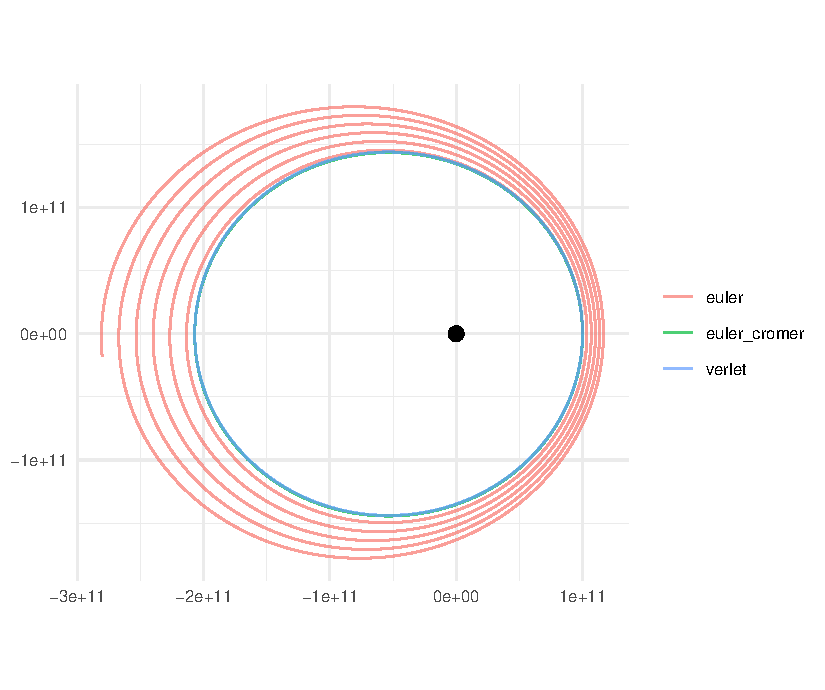
\includegraphics[width=0.85\linewidth,height=\textheight,keepaspectratio]{05-integrators_files/figure-pdf/fig-three-methods-1.pdf}

}

\caption{\label{fig-three-methods}Ten years of the same orbit with three
integrators and a six-hour step. Verlet retraces one ellipse;
Euler-Cromer stays on an ellipse of the right size but slips in phase;
Euler spirals outward.}

\end{figure}%

The picture is the one in the documentation. Now the number behind it.
The total energy of any N-body system is the kinetic energy of every
body plus the potential energy of every \emph{pair},

\begin{equation}\protect\phantomsection\label{eq-total-energy}{
E = \sum_j \tfrac12 m_j v_j^2 \;-\; \sum_{j<k} \frac{G m_j m_k}{r_{jk}},
}\end{equation}

and both are easy to compute from the output tibble. The potential
energy needs every pair at every time step, which is a self-join on
\texttt{time}:

\begin{Shaded}
\begin{Highlighting}[]
\NormalTok{total\_energy }\OtherTok{\textless{}{-}} \ControlFlowTok{function}\NormalTok{(sim, }\AttributeTok{G =}\NormalTok{ gravitational\_constant) \{}
\NormalTok{  kinetic }\OtherTok{\textless{}{-}}\NormalTok{ sim }\SpecialCharTok{|\textgreater{}}
    \FunctionTok{group\_by}\NormalTok{(time) }\SpecialCharTok{|\textgreater{}}
    \FunctionTok{summarise}\NormalTok{(}\AttributeTok{KE =} \FunctionTok{sum}\NormalTok{(}\FloatTok{0.5} \SpecialCharTok{*}\NormalTok{ mass }\SpecialCharTok{*}\NormalTok{ (vx}\SpecialCharTok{\^{}}\DecValTok{2} \SpecialCharTok{+}\NormalTok{ vy}\SpecialCharTok{\^{}}\DecValTok{2} \SpecialCharTok{+}\NormalTok{ vz}\SpecialCharTok{\^{}}\DecValTok{2}\NormalTok{)))}

\NormalTok{  potential }\OtherTok{\textless{}{-}}\NormalTok{ sim }\SpecialCharTok{|\textgreater{}}
    \FunctionTok{select}\NormalTok{(time, id, mass, x, y, z) }\SpecialCharTok{|\textgreater{}}
    \FunctionTok{inner\_join}\NormalTok{(sim }\SpecialCharTok{|\textgreater{}} \FunctionTok{select}\NormalTok{(time, }\AttributeTok{id2 =}\NormalTok{ id, }\AttributeTok{mass2 =}\NormalTok{ mass,}
                             \AttributeTok{x2 =}\NormalTok{ x, }\AttributeTok{y2 =}\NormalTok{ y, }\AttributeTok{z2 =}\NormalTok{ z),}
               \AttributeTok{by =} \StringTok{"time"}\NormalTok{, }\AttributeTok{relationship =} \StringTok{"many{-}to{-}many"}\NormalTok{) }\SpecialCharTok{|\textgreater{}}
    \FunctionTok{filter}\NormalTok{(id }\SpecialCharTok{\textless{}}\NormalTok{ id2) }\SpecialCharTok{|\textgreater{}}                       \CommentTok{\# each unordered pair once}
    \FunctionTok{mutate}\NormalTok{(}\AttributeTok{r =} \FunctionTok{sqrt}\NormalTok{((x }\SpecialCharTok{{-}}\NormalTok{ x2)}\SpecialCharTok{\^{}}\DecValTok{2} \SpecialCharTok{+}\NormalTok{ (y }\SpecialCharTok{{-}}\NormalTok{ y2)}\SpecialCharTok{\^{}}\DecValTok{2} \SpecialCharTok{+}\NormalTok{ (z }\SpecialCharTok{{-}}\NormalTok{ z2)}\SpecialCharTok{\^{}}\DecValTok{2}\NormalTok{)) }\SpecialCharTok{|\textgreater{}}
    \FunctionTok{group\_by}\NormalTok{(time) }\SpecialCharTok{|\textgreater{}}
    \FunctionTok{summarise}\NormalTok{(}\AttributeTok{PE =} \SpecialCharTok{{-}}\FunctionTok{sum}\NormalTok{(G }\SpecialCharTok{*}\NormalTok{ mass }\SpecialCharTok{*}\NormalTok{ mass2 }\SpecialCharTok{/}\NormalTok{ r))}

  \FunctionTok{inner\_join}\NormalTok{(kinetic, potential, }\AttributeTok{by =} \StringTok{"time"}\NormalTok{) }\SpecialCharTok{|\textgreater{}}
    \FunctionTok{mutate}\NormalTok{(}\AttributeTok{E =}\NormalTok{ KE }\SpecialCharTok{+}\NormalTok{ PE,}
           \AttributeTok{rel\_error =}\NormalTok{ (E }\SpecialCharTok{{-}} \FunctionTok{first}\NormalTok{(E)) }\SpecialCharTok{/} \FunctionTok{abs}\NormalTok{(}\FunctionTok{first}\NormalTok{(E)))}
\NormalTok{\}}
\end{Highlighting}
\end{Shaded}

This is what the package's \texttt{get\_energy()} computes, one row per
time step with \texttt{kinetic}, \texttt{potential}, and \texttt{energy}
columns (and it reads the softening length from the run, so the
potential matches the force law that was actually used).
\texttt{conserved\_quantities()} goes one step further and adds the
relative error \((E - E_0)/|E_0|\) as \texttt{energy\_error}, together
with the total momentum and angular momentum, which Chapter 12 uses.
Having seen the sum written out once, I will use those from here on.

\begin{Shaded}
\begin{Highlighting}[]
\NormalTok{energy }\OtherTok{\textless{}{-}}\NormalTok{ runs }\SpecialCharTok{|\textgreater{}}
  \FunctionTok{group\_by}\NormalTok{(method) }\SpecialCharTok{|\textgreater{}}
  \FunctionTok{group\_modify}\NormalTok{(}\SpecialCharTok{\textasciitilde{}} \FunctionTok{conserved\_quantities}\NormalTok{(.x)) }\SpecialCharTok{|\textgreater{}}
  \FunctionTok{ungroup}\NormalTok{()}

\NormalTok{energy }\SpecialCharTok{|\textgreater{}}
  \FunctionTok{ggplot}\NormalTok{(}\FunctionTok{aes}\NormalTok{(time }\SpecialCharTok{/}\NormalTok{ seconds\_per\_year, energy\_error)) }\SpecialCharTok{+}
  \FunctionTok{geom\_line}\NormalTok{() }\SpecialCharTok{+}
  \FunctionTok{facet\_wrap}\NormalTok{(}\SpecialCharTok{\textasciitilde{}}\NormalTok{ method, }\AttributeTok{scales =} \StringTok{"free\_y"}\NormalTok{, }\AttributeTok{ncol =} \DecValTok{1}\NormalTok{) }\SpecialCharTok{+}
  \FunctionTok{labs}\NormalTok{(}\AttributeTok{x =} \StringTok{"Years"}\NormalTok{, }\AttributeTok{y =} \StringTok{"Relative energy error"}\NormalTok{)}
\end{Highlighting}
\end{Shaded}

\begin{figure}[tbp]

\centering{

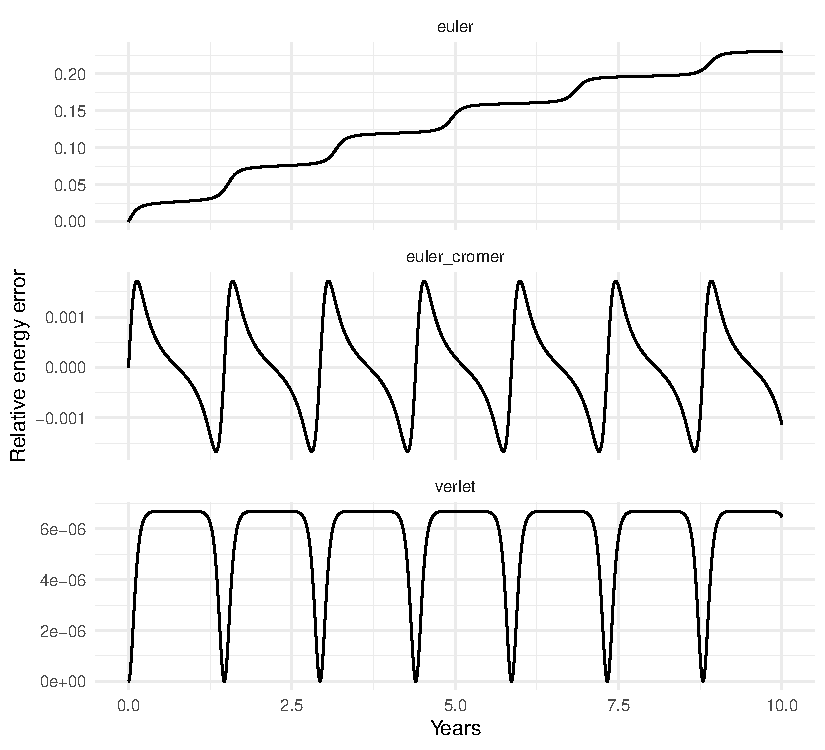
\includegraphics[width=0.9\linewidth,height=\textheight,keepaspectratio]{05-integrators_files/figure-pdf/fig-energy-drift-1.pdf}

}

\caption{\label{fig-energy-drift}Relative energy error
\((E - E_0)/|E_0|\) for the three runs. Note the different vertical
scales: Euler's error grows without limit, while the two symplectic
methods oscillate within a fixed band, with spikes at each periapsis
passage where the step is effectively largest.}

\end{figure}%

The Euler run gains tens of percent of its binding energy in ten years
and would eventually escape. The two symplectic runs show the bounded
oscillation that backward error analysis promises: the error rises and
falls once per orbit, biggest near periapsis where the planet moves
fastest and a fixed step covers the most angle, and comes back to nearly
zero each time. It does not accumulate.

\subsection{Order, measured}\label{order-measured}

The last claim to check is the order. Run Euler and Verlet at four step
sizes and record the worst energy error over two years:

\begin{Shaded}
\begin{Highlighting}[]
\NormalTok{steps }\OtherTok{\textless{}{-}}\NormalTok{ seconds\_per\_day }\SpecialCharTok{*} \FunctionTok{c}\NormalTok{(}\DecValTok{1}\NormalTok{, }\FloatTok{0.5}\NormalTok{, }\FloatTok{0.25}\NormalTok{, }\FloatTok{0.125}\NormalTok{)}

\NormalTok{convergence }\OtherTok{\textless{}{-}} \FunctionTok{bind\_rows}\NormalTok{(}\FunctionTok{lapply}\NormalTok{(}\FunctionTok{c}\NormalTok{(}\StringTok{"euler"}\NormalTok{, }\StringTok{"verlet"}\NormalTok{), }\ControlFlowTok{function}\NormalTok{(m) \{}
  \FunctionTok{bind\_rows}\NormalTok{(}\FunctionTok{lapply}\NormalTok{(steps, }\ControlFlowTok{function}\NormalTok{(dt) \{}
\NormalTok{    star\_planet }\SpecialCharTok{|\textgreater{}}
      \FunctionTok{simulate\_system}\NormalTok{(}\AttributeTok{time\_step =}\NormalTok{ dt, }\AttributeTok{duration =}\NormalTok{ seconds\_per\_year }\SpecialCharTok{*} \DecValTok{2}\NormalTok{,}
                      \AttributeTok{method =}\NormalTok{ m) }\SpecialCharTok{|\textgreater{}}
      \FunctionTok{conserved\_quantities}\NormalTok{() }\SpecialCharTok{|\textgreater{}}
      \FunctionTok{summarise}\NormalTok{(}\AttributeTok{max\_rel\_error =} \FunctionTok{max}\NormalTok{(}\FunctionTok{abs}\NormalTok{(energy\_error))) }\SpecialCharTok{|\textgreater{}}
      \FunctionTok{mutate}\NormalTok{(}\AttributeTok{method =}\NormalTok{ m, }\AttributeTok{step\_days =}\NormalTok{ dt }\SpecialCharTok{/}\NormalTok{ seconds\_per\_day)}
\NormalTok{  \}))}
\NormalTok{\}))}

\NormalTok{convergence }\SpecialCharTok{|\textgreater{}}
  \FunctionTok{group\_by}\NormalTok{(method) }\SpecialCharTok{|\textgreater{}}
  \FunctionTok{mutate}\NormalTok{(}\AttributeTok{ratio =} \FunctionTok{lag}\NormalTok{(max\_rel\_error) }\SpecialCharTok{/}\NormalTok{ max\_rel\_error) }\SpecialCharTok{|\textgreater{}}
  \FunctionTok{ungroup}\NormalTok{() }\SpecialCharTok{|\textgreater{}}
  \FunctionTok{select}\NormalTok{(method, step\_days, max\_rel\_error, ratio)}
\CommentTok{\#\textgreater{} \# A tibble: 8 x 4}
\CommentTok{\#\textgreater{}   method step\_days max\_rel\_error ratio}
\CommentTok{\#\textgreater{}   \textless{}chr\textgreater{}      \textless{}dbl\textgreater{}         \textless{}dbl\textgreater{} \textless{}dbl\textgreater{}}
\CommentTok{\#\textgreater{} 1 euler      1        0.238      NA   }
\CommentTok{\#\textgreater{} 2 euler      0.5      0.137       1.74}
\CommentTok{\#\textgreater{} 3 euler      0.25     0.0736      1.86}
\CommentTok{\#\textgreater{} 4 euler      0.125    0.0383      1.92}
\CommentTok{\#\textgreater{} 5 verlet     1        0.000107   NA   }
\CommentTok{\#\textgreater{} 6 verlet     0.5      0.0000268   4.00}
\CommentTok{\#\textgreater{} 7 verlet     0.25     0.00000669  4.00}
\CommentTok{\#\textgreater{} 8 verlet     0.125    0.00000167  4.00}
\end{Highlighting}
\end{Shaded}

Each halving of the step cuts Euler's error by about two and Verlet's by
about four: first order and second order, as derived. The ratios are not
exactly 2 and 4 because the error has higher-order pieces too, and
because the ``worst'' error for Verlet is set by the periapsis passages,
which a coarser step samples differently each time. They are close.

\section{Choosing a time step}\label{choosing-a-time-step}

Everything above gives you the tools to choose \texttt{time\_step}
sensibly rather than by habit.

\textbf{The fastest orbit sets the step.} The error in a step depends on
how much the acceleration changes during it, which is to say on how
large a fraction of an orbit the step covers. In a system with the Sun,
Earth, and the Moon, the Moon's 27-day orbit, not Earth's year, decides
the step. A good rule of thumb is a few hundred to a thousand steps per
orbit of the tightest orbit in the system: an hour for the Moon, a day
for the planets, as the package defaults suggest.

\textbf{Periapsis is where it hurts.} For an eccentric orbit the body
moves fastest at periapsis, and the angular rate there is \(h/r_p^2\),
larger than the mean rate by a factor of roughly \((1+e)/(1-e)\) when
\(e\) is substantial. A comet with \(e = 0.97\) moves through periapsis
about sixty times faster than its average, and a step that is fine at
aphelion is useless at perihelion. Chapter 13 deals with this.

\textbf{Stability is not accuracy.} For the oscillator, the Verlet map
is stable (its eigenvalues stay on the unit circle) as long as
\(\omega\Delta t < 2\), which is only about three steps per orbit.
Beyond that the solution blows up; short of it, the solution is bounded
but may be badly wrong. Do not take ``it didn't blow up'' as evidence
that the step was small enough.

\textbf{Test by halving.} The convergence table is the test. Run the
simulation, halve \texttt{time\_step}, run it again, and compare the
quantities you care about: final positions, periods, the energy band. If
the answers move by less than you care about, the step was fine. If they
move a lot, halve again. This costs a factor of two or three in compute
time once and saves you from publishing a numerical artifact.

\begin{tcolorbox}[enhanced jigsaw, arc=.35mm, bottomrule=.15mm, bottomtitle=1mm, breakable, colback=white, colbacktitle=quarto-callout-tip-color!10!white, colframe=quarto-callout-tip-color-frame, coltitle=black, left=2mm, leftrule=.75mm, opacityback=0, opacitybacktitle=0.6, rightrule=.15mm, title={Key results}, titlerule=0mm, toprule=.15mm, toptitle=1mm]

\begin{itemize}
\tightlist
\item
  Euler: first order, increases phase-space area every step, energy
  grows without bound. Educational only.
\item
  Euler-Cromer: first order, symplectic. Energy error bounded, phase
  error \(O(\Delta t)\). Fast previews.
\item
  Velocity Verlet (= Störmer = leapfrog): second order, symplectic,
  time-reversible. Energy error bounded and \(O(\Delta t^2)\). Use it.
\item
  Total energy of an N-body system:
  \(E = \sum_j \tfrac12 m_j v_j^2 - \sum_{j<k} G m_j m_k / r_{jk}\).
\item
  Choose the step from the fastest orbit in the system, check it by
  halving.
\end{itemize}

\end{tcolorbox}

\chapter{Softening: What Happens When Bodies Get
Close}\label{sec-softening}

The inverse-square force has a hole in it. As two point masses approach,
\(1/r^2\) grows without limit, and at \(r = 0\) it is infinite. Nothing
in the real universe does this, because nothing in the real universe is
a point: two stars that get close enough touch, and from then on gravity
is the least of their problems. But the simulation does not know that.
\texttt{simulate\_system()} has an argument, \texttt{softening}, whose
entire purpose is to paper over the hole. This chapter explains what the
argument does to the force law, where the formula comes from, what it
costs you when bodies are far apart, and when you should use it. The
short version: softening is a model of bodies having size, not a fix for
a time step that is too large, and it is off by default for a reason.

\section{The singularity,
numerically}\label{the-singularity-numerically}

An integrator with a fixed step assumes the acceleration does not change
much during a step. Near a close encounter that assumption fails
completely. The characteristic time of the encounter is roughly the
periapsis distance divided by the periapsis speed, and for a deep
encounter that can be minutes while the step is an hour. The integrator
then takes one enormous kick in a direction computed from a position
that is already wrong, and the result is two bodies flying apart with
far more energy than they came in with. Nothing blows up to
\texttt{NaN}; it just produces garbage that looks like physics.

Here is a deliberately bad encounter: two Sun-mass stars approaching
each other on a path that would bring them within about two-thirds of a
solar radius, which for real stars is a collision.

\begin{Shaded}
\begin{Highlighting}[]
\NormalTok{M  }\OtherTok{\textless{}{-}} \FloatTok{1e30}
\NormalTok{mu }\OtherTok{\textless{}{-}}\NormalTok{ gravitational\_constant }\SpecialCharTok{*} \DecValTok{2} \SpecialCharTok{*}\NormalTok{ M}
\NormalTok{u  }\OtherTok{\textless{}{-}} \FloatTok{1.2e5}     \CommentTok{\# initial relative speed, m/s}
\NormalTok{b  }\OtherTok{\textless{}{-}} \FloatTok{3e9}       \CommentTok{\# initial sideways offset, m}

\NormalTok{encounter }\OtherTok{\textless{}{-}} \ControlFlowTok{function}\NormalTok{(}\AttributeTok{softening =} \DecValTok{0}\NormalTok{, }\AttributeTok{time\_step =} \DecValTok{600}\NormalTok{,}
                      \AttributeTok{duration =} \DecValTok{4} \SpecialCharTok{*}\NormalTok{ seconds\_per\_day) \{}
  \FunctionTok{create\_system}\NormalTok{() }\SpecialCharTok{|\textgreater{}}
    \FunctionTok{add\_body}\NormalTok{(}\StringTok{"A"}\NormalTok{, }\AttributeTok{mass =}\NormalTok{ M, }\AttributeTok{x =} \SpecialCharTok{{-}}\FloatTok{1e10}\NormalTok{, }\AttributeTok{y =} \SpecialCharTok{{-}}\NormalTok{b }\SpecialCharTok{/} \DecValTok{2}\NormalTok{, }\AttributeTok{vx =}\NormalTok{  u }\SpecialCharTok{/} \DecValTok{2}\NormalTok{) }\SpecialCharTok{|\textgreater{}}
    \FunctionTok{add\_body}\NormalTok{(}\StringTok{"B"}\NormalTok{, }\AttributeTok{mass =}\NormalTok{ M, }\AttributeTok{x =}  \FloatTok{1e10}\NormalTok{, }\AttributeTok{y =}\NormalTok{  b }\SpecialCharTok{/} \DecValTok{2}\NormalTok{, }\AttributeTok{vx =} \SpecialCharTok{{-}}\NormalTok{u }\SpecialCharTok{/} \DecValTok{2}\NormalTok{) }\SpecialCharTok{|\textgreater{}}
    \FunctionTok{simulate\_system}\NormalTok{(}\AttributeTok{time\_step =}\NormalTok{ time\_step, }\AttributeTok{duration =}\NormalTok{ duration,}
                    \AttributeTok{softening =}\NormalTok{ softening)}
\NormalTok{\}}
\end{Highlighting}
\end{Shaded}

Before running anything, Chapter 4 tells us what should happen. From the
initial relative state we can get the eccentricity, and from the
eccentricity the periapsis distance and the angle through which the
stars should be deflected. For a hyperbola, each asymptote makes an
angle \(\arccos(-1/e)\) with the periapsis direction, so the total
deflection is \(\delta = 2\arcsin(1/e)\):

\begin{Shaded}
\begin{Highlighting}[]
\NormalTok{start }\OtherTok{\textless{}{-}} \FunctionTok{encounter}\NormalTok{(}\AttributeTok{duration =} \DecValTok{600}\NormalTok{)        }\CommentTok{\# one step: just the initial state}
\NormalTok{e0    }\OtherTok{\textless{}{-}} \FunctionTok{get\_orbital\_elements}\NormalTok{(start, }\StringTok{"B"}\NormalTok{, }\StringTok{"A"}\NormalTok{, }\AttributeTok{mu =}\NormalTok{ mu)}\SpecialCharTok{$}\NormalTok{e[}\DecValTok{1}\NormalTok{]   }\CommentTok{\# mu = G(M\_A + M\_B)}
\NormalTok{r\_p   }\OtherTok{\textless{}{-}}\NormalTok{ (b }\SpecialCharTok{*}\NormalTok{ u)}\SpecialCharTok{\^{}}\DecValTok{2} \SpecialCharTok{/}\NormalTok{ mu }\SpecialCharTok{/}\NormalTok{ (}\DecValTok{1} \SpecialCharTok{+}\NormalTok{ e0)        }\CommentTok{\# p / (1 + e), with h = b u}

\FunctionTok{c}\NormalTok{(}\AttributeTok{e =}\NormalTok{ e0, }\AttributeTok{periapsis\_solar\_radii =}\NormalTok{ r\_p }\SpecialCharTok{/} \FloatTok{6.957e8}\NormalTok{,}
  \AttributeTok{deflection\_deg =} \DecValTok{2} \SpecialCharTok{*} \FunctionTok{asin}\NormalTok{(}\DecValTok{1} \SpecialCharTok{/}\NormalTok{ e0) }\SpecialCharTok{*} \DecValTok{180} \SpecialCharTok{/}\NormalTok{ pi)}
\CommentTok{\#\textgreater{}                     e periapsis\_solar\_radii        deflection\_deg }
\CommentTok{\#\textgreater{}             1.0043512             0.6962632           169.3294587}
\end{Highlighting}
\end{Shaded}

The stars should swing around each other through about 169 degrees,
nearly reversing direction, and leave with exactly the eccentricity and
energy they arrived with. Now run it with a ten-minute step and no
softening:

\begin{Shaded}
\begin{Highlighting}[]
\NormalTok{bad }\OtherTok{\textless{}{-}} \FunctionTok{encounter}\NormalTok{(}\AttributeTok{softening =} \DecValTok{0}\NormalTok{, }\AttributeTok{time\_step =} \DecValTok{600}\NormalTok{)}

\FunctionTok{c}\NormalTok{(}\AttributeTok{e\_start =} \FunctionTok{get\_orbital\_elements}\NormalTok{(bad, }\StringTok{"B"}\NormalTok{, }\StringTok{"A"}\NormalTok{, }\AttributeTok{mu =}\NormalTok{ mu)}\SpecialCharTok{$}\NormalTok{e[}\DecValTok{1}\NormalTok{],}
  \AttributeTok{e\_end   =} \FunctionTok{get\_orbital\_elements}\NormalTok{(bad, }\StringTok{"B"}\NormalTok{, }\StringTok{"A"}\NormalTok{, }\AttributeTok{mu =}\NormalTok{ mu)}\SpecialCharTok{$}\NormalTok{e[}\FunctionTok{nrow}\NormalTok{(bad) }\SpecialCharTok{/} \DecValTok{2}\NormalTok{],}
  \AttributeTok{max\_energy\_error =} \FunctionTok{max}\NormalTok{(}\FunctionTok{abs}\NormalTok{(}\FunctionTok{conserved\_quantities}\NormalTok{(bad)}\SpecialCharTok{$}\NormalTok{energy\_error)))}
\CommentTok{\#\textgreater{}          e\_start            e\_end max\_energy\_error }
\CommentTok{\#\textgreater{}         1.004351         1.005115        21.463194}
\end{Highlighting}
\end{Shaded}

The eccentricity, which should be a constant of the motion, is not even
close, and the energy error is enormous. The time step was far too large
for the periapsis passage, and the integrator did what integrators do
with too large a step: it invented energy. The paths look like a
slingshot because that is what a huge spurious kick looks like.

\section{Plummer softening}\label{plummer-softening}

The package's remedy replaces the distance in the force law:

\[
r \;\longrightarrow\; r_{\mathrm{soft}} = \sqrt{r^2 + \varepsilon^2},
\]

so the acceleration of body \(j\) due to body \(k\) becomes

\begin{equation}\protect\phantomsection\label{eq-softened}{
\mathbf{a}_{jk} = G m_k \,\frac{\mathbf{r}_k - \mathbf{r}_j}{\left(r_{jk}^2 + \varepsilon^2\right)^{3/2}}.
}\end{equation}

The difference vector in the numerator is untouched; only the \(r^3\) in
the denominator is softened. At \(r = 0\) the acceleration is now zero,
not infinite, and its maximum magnitude, which occurs at
\(r = \varepsilon/\sqrt2\), is about \(0.38\,G m_k/\varepsilon^2\).

\begin{tcolorbox}[enhanced jigsaw, arc=.35mm, bottomrule=.15mm, bottomtitle=1mm, breakable, colback=white, colbacktitle=quarto-callout-note-color!10!white, colframe=quarto-callout-note-color-frame, coltitle=black, left=2mm, leftrule=.75mm, opacityback=0, opacitybacktitle=0.6, rightrule=.15mm, title={Where it comes from}, titlerule=0mm, toprule=.15mm, toptitle=1mm]

In 1911 H. C. Plummer was fitting the observed brightness profiles of
globular clusters and found that a density law of the form
\(\rho(r) \propto (1 + r^2/\varepsilon^2)^{-5/2}\) matched them well
(Plummer 1911). The gravitational potential of that density distribution
works out to

\[
\Phi(r) = -\frac{GM}{\sqrt{r^2 + \varepsilon^2}},
\]

a potential that looks exactly like a point mass at large \(r\) and
flattens out smoothly to a finite value at the center. Differentiating,
the acceleration is \(-d\Phi/dr = -GMr/(r^2+\varepsilon^2)^{3/2}\),
which is Equation~\ref{eq-softened}. So softening is not an ad hoc
patch: it replaces each point mass by a small Plummer sphere of scale
radius \(\varepsilon\), and the resulting force is still exactly the
gradient of a potential, which means the softened system still conserves
energy (its own softened energy) and angular momentum. When N-body
simulation of star clusters began in earnest in the 1960s, Aarseth and
others adopted the Plummer form because it was the simplest potential
that was both finite at the origin and physically interpretable (Aarseth
2003), and it has been the default ever since.

\end{tcolorbox}

Figure~\ref{fig-softened-force} shows what the softened force looks
like. Inside \(\varepsilon\) it falls to zero; outside a few
\(\varepsilon\) it is indistinguishable from the point-mass force.

\begin{Shaded}
\begin{Highlighting}[]
\FunctionTok{tibble}\NormalTok{(}\AttributeTok{x =} \FunctionTok{seq}\NormalTok{(}\FloatTok{0.05}\NormalTok{, }\DecValTok{5}\NormalTok{, }\AttributeTok{by =} \FloatTok{0.01}\NormalTok{)) }\SpecialCharTok{|\textgreater{}}
  \FunctionTok{mutate}\NormalTok{(}\AttributeTok{point\_mass =} \DecValTok{1} \SpecialCharTok{/}\NormalTok{ x}\SpecialCharTok{\^{}}\DecValTok{2}\NormalTok{,}
         \AttributeTok{softened   =}\NormalTok{ x }\SpecialCharTok{/}\NormalTok{ (}\DecValTok{1} \SpecialCharTok{+}\NormalTok{ x}\SpecialCharTok{\^{}}\DecValTok{2}\NormalTok{)}\SpecialCharTok{\^{}}\FloatTok{1.5}\NormalTok{) }\SpecialCharTok{|\textgreater{}}
\NormalTok{  tidyr}\SpecialCharTok{::}\FunctionTok{pivot\_longer}\NormalTok{(}\SpecialCharTok{{-}}\NormalTok{x, }\AttributeTok{names\_to =} \StringTok{"law"}\NormalTok{, }\AttributeTok{values\_to =} \StringTok{"a"}\NormalTok{) }\SpecialCharTok{|\textgreater{}}
  \FunctionTok{ggplot}\NormalTok{(}\FunctionTok{aes}\NormalTok{(x, a, }\AttributeTok{linetype =}\NormalTok{ law)) }\SpecialCharTok{+}
  \FunctionTok{geom\_line}\NormalTok{() }\SpecialCharTok{+}
  \FunctionTok{coord\_cartesian}\NormalTok{(}\AttributeTok{ylim =} \FunctionTok{c}\NormalTok{(}\DecValTok{0}\NormalTok{, }\DecValTok{2}\NormalTok{)) }\SpecialCharTok{+}
  \FunctionTok{labs}\NormalTok{(}\AttributeTok{x =} \FunctionTok{expression}\NormalTok{(r }\SpecialCharTok{/}\NormalTok{ epsilon), }\AttributeTok{y =} \StringTok{"Acceleration"}\NormalTok{, }\AttributeTok{linetype =} \ConstantTok{NULL}\NormalTok{)}
\end{Highlighting}
\end{Shaded}

\begin{figure}[tbp]

\centering{

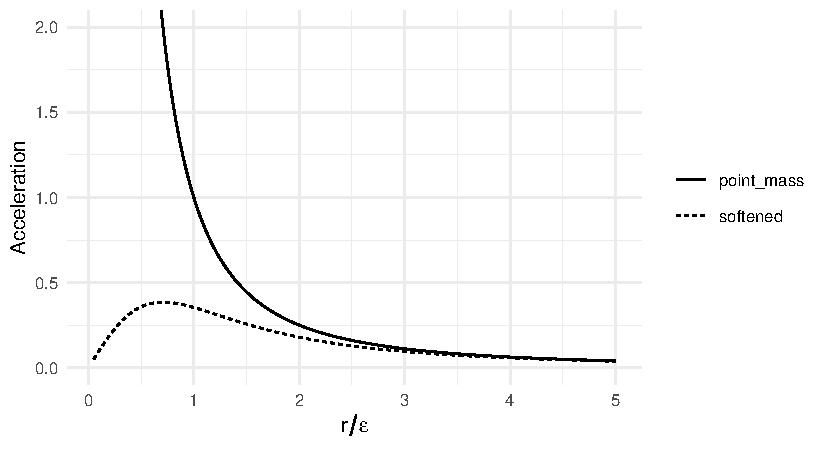
\includegraphics[width=1\linewidth,height=\textheight,keepaspectratio]{06-softening_files/figure-pdf/fig-softened-force-1.pdf}

}

\caption{\label{fig-softened-force}The softened acceleration (solid)
compared with the point-mass \(1/r^2\) law (dashed), in units where
\(Gm/\varepsilon^2 = 1\). Beyond \(r \approx 3\varepsilon\) the two
agree to a few percent.}

\end{figure}%

\section{What softening costs}\label{what-softening-costs}

The softened force is weaker than the true force at \emph{every}
distance, not just inside \(\varepsilon\). The ratio is

\begin{equation}\protect\phantomsection\label{eq-softening-error}{
\frac{a_{\mathrm{soft}}}{a} = \left(1 + \frac{\varepsilon^2}{r^2}\right)^{-3/2} \approx 1 - \frac{3}{2}\frac{\varepsilon^2}{r^2}
\qquad (r \gg \varepsilon).
}\end{equation}

For a circular orbit the period goes as the inverse square root of the
force, so softening lengthens every period by a fraction of about
\(\tfrac34\,\varepsilon^2/r^2\). Put numbers in. The documentation
suggests \texttt{softening\ =\ 1e4} (10 km) as reasonable for planetary
systems; at Earth's distance from the Sun,
\(\varepsilon/r \approx 7\times10^{-8}\) and the period changes by one
part in \(10^{14}\). You could not detect that with a million years of
simulation. At \(\varepsilon = 10^9\) m the change at 1 AU is
\(3\times10^{-5}\), about a quarter of an hour per year, which starts to
matter for precise work. At \(\varepsilon = 10^{10}\) m, a bit under a
tenth of an AU, Earth's year would be about three days too long.

The lesson is that softening is cheap as long as \(\varepsilon\) is much
smaller than every orbital separation you care about, and it is never
free. With \texttt{softening\ =\ 0}, the default, there is no error of
this kind at all, and for planetary systems, where nothing ever gets
close to anything, the default is the right choice.

\section{The encounter, softened}\label{the-encounter-softened}

Run the same encounter with the same ten-minute step and a softening
length of \(3\times10^9\) m, about four solar radii, which is a crude
way of saying ``these stars have size'':

\begin{Shaded}
\begin{Highlighting}[]
\NormalTok{soft }\OtherTok{\textless{}{-}} \FunctionTok{encounter}\NormalTok{(}\AttributeTok{softening =} \FloatTok{3e9}\NormalTok{, }\AttributeTok{time\_step =} \DecValTok{600}\NormalTok{)}

\FunctionTok{c}\NormalTok{(}\AttributeTok{e\_start =} \FunctionTok{get\_orbital\_elements}\NormalTok{(soft, }\StringTok{"B"}\NormalTok{, }\StringTok{"A"}\NormalTok{, }\AttributeTok{mu =}\NormalTok{ mu)}\SpecialCharTok{$}\NormalTok{e[}\DecValTok{1}\NormalTok{],}
  \AttributeTok{e\_end   =} \FunctionTok{get\_orbital\_elements}\NormalTok{(soft, }\StringTok{"B"}\NormalTok{, }\StringTok{"A"}\NormalTok{, }\AttributeTok{mu =}\NormalTok{ mu)}\SpecialCharTok{$}\NormalTok{e[}\FunctionTok{nrow}\NormalTok{(soft) }\SpecialCharTok{/} \DecValTok{2}\NormalTok{],}
  \AttributeTok{max\_energy\_error =} \FunctionTok{max}\NormalTok{(}\FunctionTok{abs}\NormalTok{(}\FunctionTok{conserved\_quantities}\NormalTok{(soft)}\SpecialCharTok{$}\NormalTok{energy\_error)))}
\CommentTok{\#\textgreater{}          e\_start            e\_end max\_energy\_error }
\CommentTok{\#\textgreater{}        1.0043512        1.0047221        0.0140379}
\end{Highlighting}
\end{Shaded}

Two things changed. First, the energy is now conserved to a fraction of
a percent, because the softened force varies slowly enough during the
encounter for a ten-minute step to follow it. Second, the eccentricity
after the encounter is different from the eccentricity before, \emph{and
that is correct}: the stars did not interact through a point-mass force,
so they are not on the point-mass hyperbola. Softening changed the
physics, which is what it is for. The energy diagnostic needs the same
softening, so that it computes the potential energy of the force that
was actually used. \texttt{conserved\_quantities()} reads the softening
length from the simulation output and replaces \(r\) with
\(\sqrt{r^2+\varepsilon^2}\) in the potential automatically; if you
compute the energy yourself, you have to do the same.

The third run is the honest one: no softening, and a step small enough
for the point-mass physics.

\begin{Shaded}
\begin{Highlighting}[]
\NormalTok{fine }\OtherTok{\textless{}{-}} \FunctionTok{encounter}\NormalTok{(}\AttributeTok{softening =} \DecValTok{0}\NormalTok{, }\AttributeTok{time\_step =} \DecValTok{20}\NormalTok{)}

\FunctionTok{c}\NormalTok{(}\AttributeTok{e\_start =} \FunctionTok{get\_orbital\_elements}\NormalTok{(fine, }\StringTok{"B"}\NormalTok{, }\StringTok{"A"}\NormalTok{, }\AttributeTok{mu =}\NormalTok{ mu)}\SpecialCharTok{$}\NormalTok{e[}\DecValTok{1}\NormalTok{],}
  \AttributeTok{e\_end   =} \FunctionTok{get\_orbital\_elements}\NormalTok{(fine, }\StringTok{"B"}\NormalTok{, }\StringTok{"A"}\NormalTok{, }\AttributeTok{mu =}\NormalTok{ mu)}\SpecialCharTok{$}\NormalTok{e[}\FunctionTok{nrow}\NormalTok{(fine) }\SpecialCharTok{/} \DecValTok{2}\NormalTok{],}
  \AttributeTok{max\_energy\_error =} \FunctionTok{max}\NormalTok{(}\FunctionTok{abs}\NormalTok{(}\FunctionTok{conserved\_quantities}\NormalTok{(fine)}\SpecialCharTok{$}\NormalTok{energy\_error)))}
\CommentTok{\#\textgreater{}          e\_start            e\_end max\_energy\_error }
\CommentTok{\#\textgreater{}        1.0043512        1.0043512        0.0270577}
\end{Highlighting}
\end{Shaded}

Now the eccentricity survives the encounter and the energy error is
small. That cost thirty times as many steps as the softened run, and it
is the only one of the three that answers the question ``what would two
point masses do?''

\begin{Shaded}
\begin{Highlighting}[]
\FunctionTok{bind\_rows}\NormalTok{(bad  }\SpecialCharTok{|\textgreater{}} \FunctionTok{mutate}\NormalTok{(}\AttributeTok{run =} \StringTok{"softening = 0, dt = 10 min"}\NormalTok{),}
\NormalTok{          soft }\SpecialCharTok{|\textgreater{}} \FunctionTok{mutate}\NormalTok{(}\AttributeTok{run =} \StringTok{"softening = 3e9 m, dt = 10 min"}\NormalTok{),}
\NormalTok{          fine }\SpecialCharTok{|\textgreater{}} \FunctionTok{mutate}\NormalTok{(}\AttributeTok{run =} \StringTok{"softening = 0, dt = 20 s"}\NormalTok{)) }\SpecialCharTok{|\textgreater{}}
  \FunctionTok{ggplot}\NormalTok{(}\FunctionTok{aes}\NormalTok{(x, y, }\AttributeTok{color =}\NormalTok{ id)) }\SpecialCharTok{+}
  \FunctionTok{geom\_path}\NormalTok{() }\SpecialCharTok{+}
  \FunctionTok{coord\_equal}\NormalTok{() }\SpecialCharTok{+}
  \FunctionTok{facet\_wrap}\NormalTok{(}\SpecialCharTok{\textasciitilde{}}\NormalTok{ run) }\SpecialCharTok{+}
  \FunctionTok{labs}\NormalTok{(}\AttributeTok{x =} \ConstantTok{NULL}\NormalTok{, }\AttributeTok{y =} \ConstantTok{NULL}\NormalTok{, }\AttributeTok{color =} \ConstantTok{NULL}\NormalTok{) }\SpecialCharTok{+}
  \FunctionTok{theme}\NormalTok{(}\AttributeTok{axis.text =} \FunctionTok{element\_blank}\NormalTok{())}
\end{Highlighting}
\end{Shaded}

\begin{figure}[tbp]

\centering{

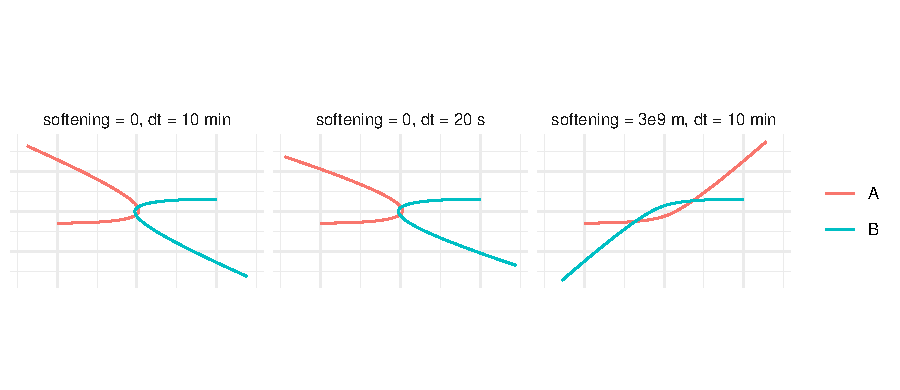
\includegraphics[width=1\linewidth,height=\textheight,keepaspectratio]{06-softening_files/figure-pdf/fig-encounter-1.pdf}

}

\caption{\label{fig-encounter}The same two stars in three runs. Left:
unsoftened, ten-minute step, a spurious kick at periapsis. Center:
softened to \(3\times 10^9\) m, same step, a smooth but physically
different encounter. Right: unsoftened, twenty-second step, the true
point-mass deflection.}

\end{figure}%

\section{When to use it}\label{when-to-use-it}

\textbf{Use softening when bodies have size and you care about what
happens when they meet.} Stars in a cluster, a planetesimal disk,
anything with many bodies and frequent close passages. Set
\(\varepsilon\) to something like the physical size of the bodies, or to
a fraction of the typical spacing, and accept that encounters closer
than \(\varepsilon\) are not being modeled correctly, because they would
not be point-mass encounters in reality either. In this regime a modest
softening also lets you use a larger time step than the closest passage
would otherwise demand, which for a thousand-body system is the
difference between a run that finishes and one that does not.

\textbf{Do not use softening to rescue a bad time step in a few-body
system.} If two planets, or a comet and the Sun, pass close and the
energy jumps, the cure is a smaller step (Chapter 13 shows how to afford
one), not a softened force that changes the answer. The only exception
is when you have decided that the close approach is a collision and you
do not care about the trajectory afterward; then softening is a cheap
way to keep the simulation from flinging things to infinity.

\textbf{Keep \(\varepsilon\) far below the smallest orbit.}
Equation~\ref{eq-softening-error} is the rule: the relative error in the
force is about \(\tfrac32(\varepsilon/r)^2\), so a softening of one
percent of the smallest orbital radius changes periods by about one part
in ten thousand. Decide what precision you need and work backward.

\textbf{Account for it in diagnostics.} The softened system conserves
the softened energy. \texttt{get\_energy()} and
\texttt{conserved\_quantities()} take the softening length from the run;
if you hand-compute energies, use the softened distance, or you will
diagnose a drift that is not there.

\begin{tcolorbox}[enhanced jigsaw, arc=.35mm, bottomrule=.15mm, bottomtitle=1mm, breakable, colback=white, colbacktitle=quarto-callout-tip-color!10!white, colframe=quarto-callout-tip-color-frame, coltitle=black, left=2mm, leftrule=.75mm, opacityback=0, opacitybacktitle=0.6, rightrule=.15mm, title={Key results}, titlerule=0mm, toprule=.15mm, toptitle=1mm]

\begin{itemize}
\tightlist
\item
  Softening replaces \(r^3\) in the force denominator with
  \((r^2+\varepsilon^2)^{3/2}\). The force is finite everywhere and zero
  at \(r = 0\).
\item
  It is the force of a Plummer sphere of scale radius \(\varepsilon\):
  still conservative, still central.
\item
  Relative error in the force at distance \(r \gg \varepsilon\): about
  \(\tfrac32(\varepsilon/r)^2\). Periods lengthen by about
  \(\tfrac34(\varepsilon/r)^2\).
\item
  Softening models bodies having size. It does not fix a time step that
  is too large for the physics you asked for.
\end{itemize}

\end{tcolorbox}

\chapter{From Orbital Elements to State Vectors}\label{sec-keplerian}

\texttt{add\_body()} wants six numbers: three for position, three for
velocity. Astronomers describe orbits with six different numbers, the
classical orbital elements, and \texttt{add\_body\_keplerian()} and
\texttt{add\_planet()} translate between the two. Chapter 4 ended with a
reason to care: the four-line Moon was on the wrong orbit because a
distance and a speed, chosen separately, do not describe the real
ellipse. The elements do. This chapter derives the translation,
implements it in plain R, checks it against the package, derives the
reverse translation, and then uses it to do two things the package does
not do on its own: put a planet where it was on a given date, and watch
an orbit's elements drift under the pull of a third body.

\section{Six numbers}\label{six-numbers}

A two-body orbit is an ellipse in a plane. Two numbers fix the ellipse's
size and shape, three fix the plane's orientation in space and the
ellipse's orientation within it, and one says where along the ellipse
the body is right now.

\begin{itemize}
\tightlist
\item
  \textbf{Semi-major axis, \(a\).} The size. Half the longest diameter,
  in meters. Sets the period through \(T = 2\pi\sqrt{a^3/\mu}\).
\item
  \textbf{Eccentricity, \(e\).} The shape. \(0\) is a circle, values
  approaching \(1\) are increasingly stretched.
\item
  \textbf{Inclination, \(i\).} The tilt of the orbital plane relative to
  the reference plane (for the solar system, the ecliptic, the plane of
  Earth's orbit). \(0°\) is flat; \(90°\) is a polar orbit.
\item
  \textbf{Longitude of the ascending node, \(\Omega\)} (\texttt{lan} in
  the package). Where the tilt points. The orbit crosses the reference
  plane twice; the \emph{ascending node} is the crossing where the body
  moves from below to above, and \(\Omega\) is the angle from the
  reference \(x\) axis to that point, measured in the reference plane.
\item
  \textbf{Argument of periapsis, \(\omega\)} (\texttt{arg\_pe}). The
  angle, measured within the orbital plane, from the ascending node to
  periapsis. It rotates the ellipse within its own plane.
\item
  \textbf{True anomaly, \(\nu\)} (\texttt{nu}). The angle from periapsis
  to the body's current position, measured in the orbital plane in the
  direction of motion. Chapter 4's orbit equation is written in terms of
  it.
\end{itemize}

All angles are in degrees in the package's arguments and in radians in
this chapter's formulas. The documentation's Keplerian Elements article
shows each element varied in turn, with pictures; what follows is the
algebra underneath those pictures.

\section{Position and velocity in the orbital
plane}\label{position-and-velocity-in-the-orbital-plane}

Set up coordinates in the orbital plane with the \(x\) axis pointing
toward periapsis and the \(y\) axis \(90°\) ahead in the direction of
motion. This is the \emph{perifocal} frame. In it the position is simply
polar coordinates with the orbit equation Equation~\ref{eq-orbit-a} for
the radius:

\begin{equation}\protect\phantomsection\label{eq-pf-position}{
r = \frac{a(1-e^2)}{1 + e\cos\nu}, \qquad
\mathbf{r}_{\mathrm{pf}} = \big(r\cos\nu,\ r\sin\nu,\ 0\big).
}\end{equation}

The velocity takes a short derivation. Differentiate the position:

\[
\dot x_{\mathrm{pf}} = \dot r\cos\nu - r\dot\nu\sin\nu, \qquad
\dot y_{\mathrm{pf}} = \dot r\sin\nu + r\dot\nu\cos\nu.
\]

We need \(\dot r\) and \(\dot\nu\). The angular momentum in polar
coordinates is \(h = r^2\dot\nu\), so \(\dot\nu = h/r^2\) and
\(r\dot\nu = h/r\). Using the orbit equation with
\(p = a(1-e^2) = h^2/\mu\),

\[
r\dot\nu = \frac{h}{r} = \frac{h(1+e\cos\nu)}{p} = \frac{\mu}{h}(1 + e\cos\nu).
\]

For \(\dot r\), differentiate \(r = p/(1+e\cos\nu)\) with respect to
time:

\[
\dot r = \frac{p\,e\sin\nu\,\dot\nu}{(1+e\cos\nu)^2} = \frac{r^2 e\sin\nu}{p}\,\dot\nu = \frac{r^2 e\sin\nu}{p}\cdot\frac{h}{r^2} = \frac{h e}{p}\sin\nu = \frac{\mu}{h}\,e\sin\nu.
\]

Substituting both into the velocity components and simplifying (the
\(e\sin\nu\cos\nu\) terms cancel in \(\dot x\), and
\(\sin^2\nu + \cos^2\nu = 1\) collapses \(\dot y\)):

\begin{equation}\protect\phantomsection\label{eq-pf-velocity}{
\dot x_{\mathrm{pf}} = -\frac{\mu}{h}\sin\nu, \qquad
\dot y_{\mathrm{pf}} = \frac{\mu}{h}\,(e + \cos\nu), \qquad
h = \sqrt{\mu\,a(1-e^2)}.
}\end{equation}

These are the formulas in the package documentation. They have a nice
interpretation: in the perifocal frame the velocity vector traces a
\emph{circle} of radius \(\mu/h\) centered at \((0, \mu e/h)\) as the
body goes around. That is Hamilton's hodograph theorem, and it is
another way of saying the eccentricity vector is conserved.

At periapsis, \(\nu = 0\) and the speed is \((\mu/h)(1+e)\); at
apoapsis, \(\nu = \pi\) and it is \((\mu/h)(1-e)\). Their ratio is
\((1+e)/(1-e)\), which for Halley's Comet (\(e = 0.967\)) is about 60.
Chapter 5's warning about periapsis is this ratio.

\section{Three rotations}\label{three-rotations}

The perifocal frame is tied to the orbit. The simulation frame is tied
to the reference plane. Getting from one to the other takes three
rotations, applied to both the position and the velocity vectors, and
the only hard part is keeping the order and the signs straight.

Start with the orbit lying in the reference plane with periapsis along
\(+x\); that is the perifocal frame itself. Then:

\begin{enumerate}
\def\labelenumi{\arabic{enumi}.}
\tightlist
\item
  Rotate about the \(z\) axis by \(\omega\). Periapsis moves away from
  the \(x\) axis; the \(x\) axis is now where the ascending node will
  be.
\item
  Rotate about the (new) \(x\) axis by \(i\). The orbital plane tilts
  out of the reference plane, hinged on the node line.
\item
  Rotate about the (original) \(z\) axis by \(\Omega\). The node line
  swings around to its proper direction.
\end{enumerate}

With the standard rotation matrices

\[
R_z(\theta) = \begin{pmatrix} \cos\theta & -\sin\theta & 0 \\ \sin\theta & \cos\theta & 0 \\ 0 & 0 & 1 \end{pmatrix}, \qquad
R_x(\theta) = \begin{pmatrix} 1 & 0 & 0 \\ 0 & \cos\theta & -\sin\theta \\ 0 & \sin\theta & \cos\theta \end{pmatrix},
\]

the combined transformation is

\begin{equation}\protect\phantomsection\label{eq-rotations}{
\mathbf{r} = R_z(\Omega)\,R_x(i)\,R_z(\omega)\,\mathbf{r}_{\mathrm{pf}}, \qquad
\mathbf{v} = R_z(\Omega)\,R_x(i)\,R_z(\omega)\,\mathbf{v}_{\mathrm{pf}}.
}\end{equation}

Matrices act right to left, so \(R_z(\omega)\) is applied first, which
matches the list above. The package documentation writes the same
product as \(R_z(-\Omega)R_x(-i)R_z(-\omega)\); the sign difference is a
convention about whether a rotation matrix rotates the vector or the
coordinate axes, and the two descriptions produce the same state vector.
The code below is the test of that claim.

Finally, the elements describe the orbit \emph{relative to the parent},
so the parent's own position and velocity are added at the end. That is
why \texttt{parent} must already be in the system, and it is what lets
\texttt{add\_planet("Moon",\ parent\ =\ "Earth")} work when Earth is
itself moving around the Sun.

\section{Implementing it}\label{implementing-it}

\begin{Shaded}
\begin{Highlighting}[]
\NormalTok{rot\_x }\OtherTok{\textless{}{-}} \ControlFlowTok{function}\NormalTok{(theta) \{}
\NormalTok{  co }\OtherTok{\textless{}{-}} \FunctionTok{cos}\NormalTok{(theta); si }\OtherTok{\textless{}{-}} \FunctionTok{sin}\NormalTok{(theta)}
  \FunctionTok{matrix}\NormalTok{(}\FunctionTok{c}\NormalTok{(}\DecValTok{1}\NormalTok{, }\DecValTok{0}\NormalTok{, }\DecValTok{0}\NormalTok{,   }\DecValTok{0}\NormalTok{, co, si,   }\DecValTok{0}\NormalTok{, }\SpecialCharTok{{-}}\NormalTok{si, co), }\AttributeTok{nrow =} \DecValTok{3}\NormalTok{)}
\NormalTok{\}}
\NormalTok{rot\_z }\OtherTok{\textless{}{-}} \ControlFlowTok{function}\NormalTok{(theta) \{}
\NormalTok{  co }\OtherTok{\textless{}{-}} \FunctionTok{cos}\NormalTok{(theta); si }\OtherTok{\textless{}{-}} \FunctionTok{sin}\NormalTok{(theta)}
  \FunctionTok{matrix}\NormalTok{(}\FunctionTok{c}\NormalTok{(co, si, }\DecValTok{0}\NormalTok{,   }\SpecialCharTok{{-}}\NormalTok{si, co, }\DecValTok{0}\NormalTok{,   }\DecValTok{0}\NormalTok{, }\DecValTok{0}\NormalTok{, }\DecValTok{1}\NormalTok{), }\AttributeTok{nrow =} \DecValTok{3}\NormalTok{)}
\NormalTok{\}}

\NormalTok{keplerian\_to\_state }\OtherTok{\textless{}{-}} \ControlFlowTok{function}\NormalTok{(a, }\AttributeTok{e =} \DecValTok{0}\NormalTok{, }\AttributeTok{i =} \DecValTok{0}\NormalTok{, }\AttributeTok{lan =} \DecValTok{0}\NormalTok{, }\AttributeTok{arg\_pe =} \DecValTok{0}\NormalTok{,}
                               \AttributeTok{nu =} \DecValTok{0}\NormalTok{, mu) \{}
\NormalTok{  rad }\OtherTok{\textless{}{-}}\NormalTok{ pi }\SpecialCharTok{/} \DecValTok{180}
\NormalTok{  i }\OtherTok{\textless{}{-}}\NormalTok{ i }\SpecialCharTok{*}\NormalTok{ rad; lan }\OtherTok{\textless{}{-}}\NormalTok{ lan }\SpecialCharTok{*}\NormalTok{ rad; w }\OtherTok{\textless{}{-}}\NormalTok{ arg\_pe }\SpecialCharTok{*}\NormalTok{ rad; nu }\OtherTok{\textless{}{-}}\NormalTok{ nu }\SpecialCharTok{*}\NormalTok{ rad}

\NormalTok{  p }\OtherTok{\textless{}{-}}\NormalTok{ a }\SpecialCharTok{*}\NormalTok{ (}\DecValTok{1} \SpecialCharTok{{-}}\NormalTok{ e}\SpecialCharTok{\^{}}\DecValTok{2}\NormalTok{)}
\NormalTok{  h }\OtherTok{\textless{}{-}} \FunctionTok{sqrt}\NormalTok{(mu }\SpecialCharTok{*}\NormalTok{ p)}
\NormalTok{  r }\OtherTok{\textless{}{-}}\NormalTok{ p }\SpecialCharTok{/}\NormalTok{ (}\DecValTok{1} \SpecialCharTok{+}\NormalTok{ e }\SpecialCharTok{*} \FunctionTok{cos}\NormalTok{(nu))}

\NormalTok{  r\_pf }\OtherTok{\textless{}{-}} \FunctionTok{c}\NormalTok{(r }\SpecialCharTok{*} \FunctionTok{cos}\NormalTok{(nu), r }\SpecialCharTok{*} \FunctionTok{sin}\NormalTok{(nu), }\DecValTok{0}\NormalTok{)}
\NormalTok{  v\_pf }\OtherTok{\textless{}{-}} \FunctionTok{c}\NormalTok{(}\SpecialCharTok{{-}}\NormalTok{mu }\SpecialCharTok{/}\NormalTok{ h }\SpecialCharTok{*} \FunctionTok{sin}\NormalTok{(nu), mu }\SpecialCharTok{/}\NormalTok{ h }\SpecialCharTok{*}\NormalTok{ (e }\SpecialCharTok{+} \FunctionTok{cos}\NormalTok{(nu)), }\DecValTok{0}\NormalTok{)}

\NormalTok{  Q }\OtherTok{\textless{}{-}} \FunctionTok{rot\_z}\NormalTok{(lan) }\SpecialCharTok{\%*\%} \FunctionTok{rot\_x}\NormalTok{(i) }\SpecialCharTok{\%*\%} \FunctionTok{rot\_z}\NormalTok{(w)}
\NormalTok{  r\_in }\OtherTok{\textless{}{-}} \FunctionTok{as.vector}\NormalTok{(Q }\SpecialCharTok{\%*\%}\NormalTok{ r\_pf)}
\NormalTok{  v\_in }\OtherTok{\textless{}{-}} \FunctionTok{as.vector}\NormalTok{(Q }\SpecialCharTok{\%*\%}\NormalTok{ v\_pf)}

  \FunctionTok{tibble}\NormalTok{(}\AttributeTok{x =}\NormalTok{ r\_in[}\DecValTok{1}\NormalTok{], }\AttributeTok{y =}\NormalTok{ r\_in[}\DecValTok{2}\NormalTok{], }\AttributeTok{z =}\NormalTok{ r\_in[}\DecValTok{3}\NormalTok{],}
         \AttributeTok{vx =}\NormalTok{ v\_in[}\DecValTok{1}\NormalTok{], }\AttributeTok{vy =}\NormalTok{ v\_in[}\DecValTok{2}\NormalTok{], }\AttributeTok{vz =}\NormalTok{ v\_in[}\DecValTok{3}\NormalTok{])}
\NormalTok{\}}
\end{Highlighting}
\end{Shaded}

(\texttt{matrix()} fills column by column, which is why the entries in
\texttt{rot\_x()} and \texttt{rot\_z()} are listed one column at a
time.) Now a test against the package, using Mars with all six elements
non-trivial:

\begin{Shaded}
\begin{Highlighting}[]
\NormalTok{mars }\OtherTok{\textless{}{-}} \FunctionTok{list}\NormalTok{(}\AttributeTok{a =}\NormalTok{ distance\_mars\_sun, }\AttributeTok{e =} \FloatTok{0.0934}\NormalTok{, }\AttributeTok{i =} \FloatTok{1.85}\NormalTok{,}
             \AttributeTok{lan =} \FloatTok{49.6}\NormalTok{, }\AttributeTok{arg\_pe =} \FloatTok{286.5}\NormalTok{, }\AttributeTok{nu =} \DecValTok{120}\NormalTok{)}

\NormalTok{from\_package }\OtherTok{\textless{}{-}} \FunctionTok{create\_system}\NormalTok{() }\SpecialCharTok{|\textgreater{}}
  \FunctionTok{add\_sun}\NormalTok{() }\SpecialCharTok{|\textgreater{}}
  \FunctionTok{add\_body\_keplerian}\NormalTok{(}\StringTok{"Mars"}\NormalTok{, }\AttributeTok{mass =}\NormalTok{ mass\_mars, }\AttributeTok{parent =} \StringTok{"Sun"}\NormalTok{,}
                     \AttributeTok{a =}\NormalTok{ mars}\SpecialCharTok{$}\NormalTok{a, }\AttributeTok{e =}\NormalTok{ mars}\SpecialCharTok{$}\NormalTok{e, }\AttributeTok{i =}\NormalTok{ mars}\SpecialCharTok{$}\NormalTok{i,}
                     \AttributeTok{lan =}\NormalTok{ mars}\SpecialCharTok{$}\NormalTok{lan, }\AttributeTok{arg\_pe =}\NormalTok{ mars}\SpecialCharTok{$}\NormalTok{arg\_pe, }\AttributeTok{nu =}\NormalTok{ mars}\SpecialCharTok{$}\NormalTok{nu) }\SpecialCharTok{|\textgreater{}}
  \FunctionTok{get\_bodies}\NormalTok{() }\SpecialCharTok{|\textgreater{}}
  \FunctionTok{filter}\NormalTok{(id }\SpecialCharTok{==} \StringTok{"Mars"}\NormalTok{) }\SpecialCharTok{|\textgreater{}}
  \FunctionTok{select}\NormalTok{(x, y, z, vx, vy, vz)}

\NormalTok{by\_hand }\OtherTok{\textless{}{-}} \FunctionTok{keplerian\_to\_state}\NormalTok{(}\AttributeTok{a =}\NormalTok{ mars}\SpecialCharTok{$}\NormalTok{a, }\AttributeTok{e =}\NormalTok{ mars}\SpecialCharTok{$}\NormalTok{e, }\AttributeTok{i =}\NormalTok{ mars}\SpecialCharTok{$}\NormalTok{i,}
                              \AttributeTok{lan =}\NormalTok{ mars}\SpecialCharTok{$}\NormalTok{lan, }\AttributeTok{arg\_pe =}\NormalTok{ mars}\SpecialCharTok{$}\NormalTok{arg\_pe,}
                              \AttributeTok{nu =}\NormalTok{ mars}\SpecialCharTok{$}\NormalTok{nu,}
                              \AttributeTok{mu =}\NormalTok{ gravitational\_constant }\SpecialCharTok{*}\NormalTok{ mass\_sun)}

\FunctionTok{bind\_rows}\NormalTok{(}\AttributeTok{package =}\NormalTok{ from\_package, }\AttributeTok{by\_hand =}\NormalTok{ by\_hand, }\AttributeTok{.id =} \StringTok{"source"}\NormalTok{)}
\CommentTok{\#\textgreater{} \# A tibble: 2 x 7}
\CommentTok{\#\textgreater{}   source              x             y           z      vx    vy    vz}
\CommentTok{\#\textgreater{}   \textless{}chr\textgreater{}           \textless{}dbl\textgreater{}         \textless{}dbl\textgreater{}       \textless{}dbl\textgreater{}   \textless{}dbl\textgreater{} \textless{}dbl\textgreater{} \textless{}dbl\textgreater{}}
\CommentTok{\#\textgreater{} 1 package {-}25114100376. 235578953124. 5549391368. {-}23180. {-}512.  559.}
\CommentTok{\#\textgreater{} 2 by\_hand {-}25114100376. 235578953124. 5549391368. {-}23180. {-}512.  559.}
\end{Highlighting}
\end{Shaded}

\begin{Shaded}
\begin{Highlighting}[]
\FunctionTok{max}\NormalTok{(}\FunctionTok{abs}\NormalTok{(}\FunctionTok{as.numeric}\NormalTok{(from\_package) }\SpecialCharTok{{-}} \FunctionTok{as.numeric}\NormalTok{(by\_hand)) }\SpecialCharTok{/}
      \FunctionTok{abs}\NormalTok{(}\FunctionTok{as.numeric}\NormalTok{(by\_hand)))}
\CommentTok{\#\textgreater{} [1] 3.553888e{-}15}
\end{Highlighting}
\end{Shaded}

The two agree to floating-point precision, which settles the sign
convention. One detail worth noticing: the gravitational parameter I
passed is \(\mu = GM_{\odot}\), the parent's mass alone, which is what
\texttt{add\_body\_keplerian()} uses. For Mars the difference from
\(G(M_\odot + m_{\mathrm{Mars}})\) is three parts in ten million. For
the Moon it is not negligible, and we will come back to it.

\section{The inverse problem}\label{the-inverse-problem}

Going the other way, from a state vector to elements, is the step that
tells you what orbit a simulated body is \emph{actually} on, and every
piece of it was derived in Chapter 4. Given relative position
\(\mathbf{r}\) and velocity \(\mathbf{v}\):

\begin{itemize}
\tightlist
\item
  \(\mathbf{h} = \mathbf{r}\times\mathbf{v}\) is normal to the orbital
  plane, so \(\cos i = h_z/h\).
\item
  The \emph{node vector}
  \(\mathbf{n} = \hat{\mathbf{z}}\times\mathbf{h}\) lies along the line
  of nodes, pointing to the ascending node, so
  \(\Omega = \operatorname{atan2}(n_y, n_x)\).
\item
  The eccentricity vector
  \(\mathbf{e} = (\mathbf{v}\times\mathbf{h})/\mu - \mathbf{r}/r\)
  points to periapsis, so \(\omega\) is the angle from \(\mathbf{n}\) to
  \(\mathbf{e}\), and \(\nu\) is the angle from \(\mathbf{e}\) to
  \(\mathbf{r}\), both measured in the orbital plane.
\item
  Vis-viva, solved for \(a\): \(a = 1/(2/r - v^2/\mu)\).
\end{itemize}

The angles in the orbital plane need a sign, which comes from whether
the cross product of the two vectors points along \(\mathbf{h}\) or
against it. Two degenerate cases need a convention: a flat orbit has no
ascending node (take \(\mathbf{n} = \hat{\mathbf{x}}\), so \(\omega\)
becomes the angle from the \(x\) axis to periapsis), and a circular
orbit has no periapsis (take \(\mathbf{e}\) along \(\mathbf{n}\), so
\(\nu\) is measured from the node).

\begin{Shaded}
\begin{Highlighting}[]
\NormalTok{state\_to\_elements }\OtherTok{\textless{}{-}} \ControlFlowTok{function}\NormalTok{(x, y, z, vx, vy, vz, mu) \{}
\NormalTok{  cross }\OtherTok{\textless{}{-}} \ControlFlowTok{function}\NormalTok{(a, b) }\FunctionTok{c}\NormalTok{(a[}\DecValTok{2}\NormalTok{] }\SpecialCharTok{*}\NormalTok{ b[}\DecValTok{3}\NormalTok{] }\SpecialCharTok{{-}}\NormalTok{ a[}\DecValTok{3}\NormalTok{] }\SpecialCharTok{*}\NormalTok{ b[}\DecValTok{2}\NormalTok{],}
\NormalTok{                            a[}\DecValTok{3}\NormalTok{] }\SpecialCharTok{*}\NormalTok{ b[}\DecValTok{1}\NormalTok{] }\SpecialCharTok{{-}}\NormalTok{ a[}\DecValTok{1}\NormalTok{] }\SpecialCharTok{*}\NormalTok{ b[}\DecValTok{3}\NormalTok{],}
\NormalTok{                            a[}\DecValTok{1}\NormalTok{] }\SpecialCharTok{*}\NormalTok{ b[}\DecValTok{2}\NormalTok{] }\SpecialCharTok{{-}}\NormalTok{ a[}\DecValTok{2}\NormalTok{] }\SpecialCharTok{*}\NormalTok{ b[}\DecValTok{1}\NormalTok{])}
\NormalTok{  norm  }\OtherTok{\textless{}{-}} \ControlFlowTok{function}\NormalTok{(a) }\FunctionTok{sqrt}\NormalTok{(}\FunctionTok{sum}\NormalTok{(a}\SpecialCharTok{\^{}}\DecValTok{2}\NormalTok{))}
\NormalTok{  deg   }\OtherTok{\textless{}{-}} \ControlFlowTok{function}\NormalTok{(theta) (theta }\SpecialCharTok{*} \DecValTok{180} \SpecialCharTok{/}\NormalTok{ pi) }\SpecialCharTok{\%\%} \DecValTok{360}

\NormalTok{  r }\OtherTok{\textless{}{-}} \FunctionTok{c}\NormalTok{(x, y, z); v }\OtherTok{\textless{}{-}} \FunctionTok{c}\NormalTok{(vx, vy, vz)}
\NormalTok{  h }\OtherTok{\textless{}{-}} \FunctionTok{cross}\NormalTok{(r, v)}
\NormalTok{  n }\OtherTok{\textless{}{-}} \FunctionTok{cross}\NormalTok{(}\FunctionTok{c}\NormalTok{(}\DecValTok{0}\NormalTok{, }\DecValTok{0}\NormalTok{, }\DecValTok{1}\NormalTok{), h)}
\NormalTok{  e\_vec }\OtherTok{\textless{}{-}} \FunctionTok{cross}\NormalTok{(v, h) }\SpecialCharTok{/}\NormalTok{ mu }\SpecialCharTok{{-}}\NormalTok{ r }\SpecialCharTok{/} \FunctionTok{norm}\NormalTok{(r)}
\NormalTok{  e }\OtherTok{\textless{}{-}} \FunctionTok{norm}\NormalTok{(e\_vec)}
\NormalTok{  a }\OtherTok{\textless{}{-}} \DecValTok{1} \SpecialCharTok{/}\NormalTok{ (}\DecValTok{2} \SpecialCharTok{/} \FunctionTok{norm}\NormalTok{(r) }\SpecialCharTok{{-}} \FunctionTok{sum}\NormalTok{(v}\SpecialCharTok{\^{}}\DecValTok{2}\NormalTok{) }\SpecialCharTok{/}\NormalTok{ mu)}
\NormalTok{  i }\OtherTok{\textless{}{-}} \FunctionTok{acos}\NormalTok{(h[}\DecValTok{3}\NormalTok{] }\SpecialCharTok{/} \FunctionTok{norm}\NormalTok{(h))}

  \ControlFlowTok{if}\NormalTok{ (}\FunctionTok{norm}\NormalTok{(n) }\SpecialCharTok{\textless{}} \FloatTok{1e{-}12} \SpecialCharTok{*} \FunctionTok{norm}\NormalTok{(h)) n }\OtherTok{\textless{}{-}} \FunctionTok{c}\NormalTok{(}\DecValTok{1}\NormalTok{, }\DecValTok{0}\NormalTok{, }\DecValTok{0}\NormalTok{)       }\CommentTok{\# flat orbit}
\NormalTok{  e\_dir }\OtherTok{\textless{}{-}} \ControlFlowTok{if}\NormalTok{ (e }\SpecialCharTok{\textgreater{}} \FloatTok{1e{-}12}\NormalTok{) e\_vec }\SpecialCharTok{/}\NormalTok{ e }\ControlFlowTok{else}\NormalTok{ n }\SpecialCharTok{/} \FunctionTok{norm}\NormalTok{(n)   }\CommentTok{\# circular orbit}
\NormalTok{  h\_hat }\OtherTok{\textless{}{-}}\NormalTok{ h }\SpecialCharTok{/} \FunctionTok{norm}\NormalTok{(h)}

\NormalTok{  lan    }\OtherTok{\textless{}{-}} \FunctionTok{atan2}\NormalTok{(n[}\DecValTok{2}\NormalTok{], n[}\DecValTok{1}\NormalTok{])}
\NormalTok{  arg\_pe }\OtherTok{\textless{}{-}} \FunctionTok{atan2}\NormalTok{(}\FunctionTok{sum}\NormalTok{(}\FunctionTok{cross}\NormalTok{(n, e\_dir) }\SpecialCharTok{*}\NormalTok{ h\_hat), }\FunctionTok{sum}\NormalTok{(n }\SpecialCharTok{*}\NormalTok{ e\_dir))}
\NormalTok{  nu     }\OtherTok{\textless{}{-}} \FunctionTok{atan2}\NormalTok{(}\FunctionTok{sum}\NormalTok{(}\FunctionTok{cross}\NormalTok{(e\_dir, r) }\SpecialCharTok{*}\NormalTok{ h\_hat), }\FunctionTok{sum}\NormalTok{(e\_dir }\SpecialCharTok{*}\NormalTok{ r))}

  \FunctionTok{tibble}\NormalTok{(}\AttributeTok{a =}\NormalTok{ a, }\AttributeTok{e =}\NormalTok{ e, }\AttributeTok{i =} \FunctionTok{deg}\NormalTok{(i), }\AttributeTok{lan =} \FunctionTok{deg}\NormalTok{(lan),}
         \AttributeTok{arg\_pe =} \FunctionTok{deg}\NormalTok{(arg\_pe), }\AttributeTok{nu =} \FunctionTok{deg}\NormalTok{(nu))}
\NormalTok{\}}
\end{Highlighting}
\end{Shaded}

Round trip:

\begin{Shaded}
\begin{Highlighting}[]
\FunctionTok{state\_to\_elements}\NormalTok{(by\_hand}\SpecialCharTok{$}\NormalTok{x, by\_hand}\SpecialCharTok{$}\NormalTok{y, by\_hand}\SpecialCharTok{$}\NormalTok{z,}
\NormalTok{                  by\_hand}\SpecialCharTok{$}\NormalTok{vx, by\_hand}\SpecialCharTok{$}\NormalTok{vy, by\_hand}\SpecialCharTok{$}\NormalTok{vz,}
                  \AttributeTok{mu =}\NormalTok{ gravitational\_constant }\SpecialCharTok{*}\NormalTok{ mass\_sun)}
\CommentTok{\#\textgreater{} \# A tibble: 1 x 6}
\CommentTok{\#\textgreater{}              a      e     i   lan arg\_pe    nu}
\CommentTok{\#\textgreater{}          \textless{}dbl\textgreater{}  \textless{}dbl\textgreater{} \textless{}dbl\textgreater{} \textless{}dbl\textgreater{}  \textless{}dbl\textgreater{} \textless{}dbl\textgreater{}}
\CommentTok{\#\textgreater{} 1 227900000000 0.0934  1.85  49.6   286.  120.}
\end{Highlighting}
\end{Shaded}

Mars's elements come back. Now the question Chapter 4 left open: what
orbit was the four-line Moon on?

\begin{Shaded}
\begin{Highlighting}[]
\FunctionTok{state\_to\_elements}\NormalTok{(distance\_earth\_moon, }\DecValTok{0}\NormalTok{, }\DecValTok{0}\NormalTok{, }\DecValTok{0}\NormalTok{, speed\_moon, }\DecValTok{0}\NormalTok{,}
                  \AttributeTok{mu =}\NormalTok{ gravitational\_constant }\SpecialCharTok{*}\NormalTok{ (mass\_earth }\SpecialCharTok{+}\NormalTok{ mass\_moon))}
\CommentTok{\#\textgreater{} \# A tibble: 1 x 6}
\CommentTok{\#\textgreater{}            a       e     i   lan arg\_pe    nu}
\CommentTok{\#\textgreater{}        \textless{}dbl\textgreater{}   \textless{}dbl\textgreater{} \textless{}dbl\textgreater{} \textless{}dbl\textgreater{}  \textless{}dbl\textgreater{} \textless{}dbl\textgreater{}}
\CommentTok{\#\textgreater{} 1 382513625. 0.00493     0     0    180   180}
\end{Highlighting}
\end{Shaded}

A nearly circular orbit, starting at apoapsis (\(\nu = 180°\)), with a
semi-major axis a little under 384,400 km, exactly as Chapter 4 computed
by hand.

This inverse conversion is what \texttt{get\_orbital\_elements()} does,
for a whole simulation at once: it takes the position and velocity of a
body relative to a parent at every time step and returns the six
elements, plus the period. Its default \(\mu\) is
\(GM_{\mathrm{parent}}\), matching \texttt{add\_body\_keplerian()}, so
the round trip is exact:

\begin{Shaded}
\begin{Highlighting}[]
\NormalTok{mars\_check }\OtherTok{\textless{}{-}} \FunctionTok{create\_system}\NormalTok{() }\SpecialCharTok{|\textgreater{}}
  \FunctionTok{add\_sun}\NormalTok{() }\SpecialCharTok{|\textgreater{}}
  \FunctionTok{add\_body\_keplerian}\NormalTok{(}\StringTok{"Mars"}\NormalTok{, }\AttributeTok{mass =}\NormalTok{ mass\_mars, }\AttributeTok{parent =} \StringTok{"Sun"}\NormalTok{,}
                     \AttributeTok{a =}\NormalTok{ mars}\SpecialCharTok{$}\NormalTok{a, }\AttributeTok{e =}\NormalTok{ mars}\SpecialCharTok{$}\NormalTok{e, }\AttributeTok{i =}\NormalTok{ mars}\SpecialCharTok{$}\NormalTok{i,}
                     \AttributeTok{lan =}\NormalTok{ mars}\SpecialCharTok{$}\NormalTok{lan, }\AttributeTok{arg\_pe =}\NormalTok{ mars}\SpecialCharTok{$}\NormalTok{arg\_pe, }\AttributeTok{nu =}\NormalTok{ mars}\SpecialCharTok{$}\NormalTok{nu) }\SpecialCharTok{|\textgreater{}}
  \FunctionTok{simulate\_system}\NormalTok{(}\AttributeTok{time\_step =}\NormalTok{ seconds\_per\_day, }\AttributeTok{duration =}\NormalTok{ seconds\_per\_day)}

\FunctionTok{get\_orbital\_elements}\NormalTok{(mars\_check, }\StringTok{"Mars"}\NormalTok{, }\StringTok{"Sun"}\NormalTok{)[}\DecValTok{1}\NormalTok{, ]}
\CommentTok{\#\textgreater{} \# A tibble: 1 x 8}
\CommentTok{\#\textgreater{}    time             a      e     i   lan arg\_pe    nu    period}
\CommentTok{\#\textgreater{}   \textless{}dbl\textgreater{}         \textless{}dbl\textgreater{}  \textless{}dbl\textgreater{} \textless{}dbl\textgreater{} \textless{}dbl\textgreater{}  \textless{}dbl\textgreater{} \textless{}dbl\textgreater{}     \textless{}dbl\textgreater{}}
\CommentTok{\#\textgreater{} 1     0 227900000000. 0.0934  1.85  49.6   286.  120. 59330240.}
\end{Highlighting}
\end{Shaded}

The function is \texttt{state\_to\_elements()} with the bookkeeping
done: the relative state, the join on time, the degenerate cases, and a
\texttt{mu} argument when you want the two-body value. From here on the
book uses it.

\section{The Moon on its real orbit}\label{the-moon-on-its-real-orbit}

The real Moon's orbit has \(a = 384{,}400\) km, \(e = 0.0549\), and
\(i = 5.15°\) to the ecliptic, and
\texttt{add\_planet("Moon",\ parent\ =\ "Earth")} builds it from those
elements. Earth and the Moon are the one pair in the solar system where
the secondary's mass is not negligible, and the conversion uses
\(\mu = GM_{\mathrm{parent}}\), so it is worth checking what orbit the
package actually produces. The simulation always uses both masses, so
the orbit the Moon follows is a two-body orbit with
\(\mu = G(M_\oplus + m_{\mathrm{Moon}})\), and
\texttt{get\_orbital\_elements()} with that \(\mu\) tells us its true
semi-major axis:

\begin{Shaded}
\begin{Highlighting}[]
\NormalTok{em }\OtherTok{\textless{}{-}} \FunctionTok{create\_system}\NormalTok{() }\SpecialCharTok{|\textgreater{}}
  \FunctionTok{add\_body}\NormalTok{(}\StringTok{"Earth"}\NormalTok{, }\AttributeTok{mass =}\NormalTok{ mass\_earth) }\SpecialCharTok{|\textgreater{}}
  \FunctionTok{add\_planet}\NormalTok{(}\StringTok{"Moon"}\NormalTok{, }\AttributeTok{parent =} \StringTok{"Earth"}\NormalTok{)}

\NormalTok{em\_sim }\OtherTok{\textless{}{-}} \FunctionTok{simulate\_system}\NormalTok{(em, }\AttributeTok{time\_step =}\NormalTok{ seconds\_per\_hour,}
                          \AttributeTok{duration =}\NormalTok{ seconds\_per\_day }\SpecialCharTok{*} \DecValTok{30}\NormalTok{)}
\NormalTok{mu\_em  }\OtherTok{\textless{}{-}}\NormalTok{ gravitational\_constant }\SpecialCharTok{*}\NormalTok{ (mass\_earth }\SpecialCharTok{+}\NormalTok{ mass\_moon)}

\NormalTok{actual }\OtherTok{\textless{}{-}} \FunctionTok{get\_orbital\_elements}\NormalTok{(em\_sim, }\StringTok{"Moon"}\NormalTok{, }\StringTok{"Earth"}\NormalTok{, }\AttributeTok{mu =}\NormalTok{ mu\_em)[}\DecValTok{1}\NormalTok{, ]}
\NormalTok{actual}
\CommentTok{\#\textgreater{} \# A tibble: 1 x 8}
\CommentTok{\#\textgreater{}    time          a      e     i   lan arg\_pe       nu   period}
\CommentTok{\#\textgreater{}   \textless{}dbl\textgreater{}      \textless{}dbl\textgreater{}  \textless{}dbl\textgreater{} \textless{}dbl\textgreater{} \textless{}dbl\textgreater{}  \textless{}dbl\textgreater{}    \textless{}dbl\textgreater{}    \textless{}dbl\textgreater{}}
\CommentTok{\#\textgreater{} 1     0 379258886. 0.0421  5.15  125.   318. 1.01e{-}13 2310295.}
\end{Highlighting}
\end{Shaded}

\begin{Shaded}
\begin{Highlighting}[]
\FunctionTok{c}\NormalTok{(}\AttributeTok{a\_ratio =}\NormalTok{ actual}\SpecialCharTok{$}\NormalTok{a }\SpecialCharTok{/} \FloatTok{3.844e8}\NormalTok{,}
  \AttributeTok{T\_predicted\_days =} \DecValTok{2} \SpecialCharTok{*}\NormalTok{ pi }\SpecialCharTok{*} \FunctionTok{sqrt}\NormalTok{(actual}\SpecialCharTok{$}\NormalTok{a}\SpecialCharTok{\^{}}\DecValTok{3} \SpecialCharTok{/}\NormalTok{ mu\_em) }\SpecialCharTok{/}\NormalTok{ seconds\_per\_day)}
\CommentTok{\#\textgreater{}          a\_ratio T\_predicted\_days }
\CommentTok{\#\textgreater{}        0.9866256       26.7395241}
\end{Highlighting}
\end{Shaded}

The ratio is not 1. The velocity the conversion assigned is right for
\(\mu = GM_\oplus\) but slightly too small for the \(\mu\) the
simulation actually runs with, so the Moon settles onto a slightly
smaller, faster orbit, with a period a couple of percent short of the
real 27.32 days. The simulation confirms it:

\begin{Shaded}
\begin{Highlighting}[]
\FunctionTok{measure\_period}\NormalTok{(em\_sim, }\StringTok{"Moon"}\NormalTok{, }\StringTok{"Earth"}\NormalTok{) }\SpecialCharTok{/}\NormalTok{ seconds\_per\_day}
\CommentTok{\#\textgreater{} [1] 26.74042}
\end{Highlighting}
\end{Shaded}

If you need the Moon's period right to better than a percent, build it
with \texttt{keplerian\_to\_state()} using the combined \(\mu\) and pass
the result to \texttt{add\_body()}; \texttt{measure\_period()} then
returns the real 27.32 days. For every other body in the solar system
the question does not arise: the heaviest planet is a thousandth of the
Sun, and the error is a twentieth of a percent in its period.

\section{Where is Mars today? Kepler's
equation}\label{where-is-mars-today-keplers-equation}

The elements fix the orbit, and \(\nu\) fixes the position on it, but
\(\nu\) is not what an ephemeris gives you. An ephemeris gives you the
\emph{time of perihelion passage} or, equivalently, the \emph{mean
anomaly} \(M\) at some epoch, and converting a time into a true anomaly
is a problem Kepler himself posed and could not solve in closed form.
Nobody can; it has to be done numerically. The package starts every body
at \(\nu = 0\) by default and lets you set \texttt{nu} yourself, so if
you want the planets where they were on a particular date, this is the
calculation you have to do.

Define the mean anomaly as the angle a body would have moved through if
it went around uniformly:

\[
M = \frac{2\pi}{T}\,(t - t_p) = \sqrt{\frac{\mu}{a^3}}\,(t - t_p),
\]

where \(t_p\) is the time of periapsis. The link between \(M\) and
\(\nu\) goes through a third angle, the \emph{eccentric anomaly} \(E\),
defined geometrically: draw the circle of radius \(a\) that
circumscribes the ellipse, project the body's position straight up
(perpendicular to the major axis) onto that circle, and \(E\) is the
angle of that projected point from the center of the ellipse. Standard
ellipse geometry then gives

\begin{equation}\protect\phantomsection\label{eq-eccentric-anomaly}{
r = a(1 - e\cos E), \qquad
\tan\frac{\nu}{2} = \sqrt{\frac{1+e}{1-e}}\,\tan\frac{E}{2}.
}\end{equation}

The area swept from periapsis, computed in the auxiliary circle and
scaled by \(b/a\), comes out to \(\tfrac12 ab\,(E - e\sin E)\). Kepler's
second law says the area swept is also
\(\pi ab \cdot (t-t_p)/T = \tfrac12 ab\,M\). Equating them:

\begin{equation}\protect\phantomsection\label{eq-kepler-equation}{
M = E - e\sin E.
}\end{equation}

This is \textbf{Kepler's equation}. Given \(M\), it has to be solved for
\(E\), and since \(E\) appears both bare and inside a sine there is no
algebraic solution. Newton's method does it in a handful of iterations
for any \(e < 1\):

\begin{Shaded}
\begin{Highlighting}[]
\NormalTok{solve\_kepler }\OtherTok{\textless{}{-}} \ControlFlowTok{function}\NormalTok{(M, e, }\AttributeTok{tol =} \FloatTok{1e{-}12}\NormalTok{) \{}
\NormalTok{  E }\OtherTok{\textless{}{-}} \ControlFlowTok{if}\NormalTok{ (e }\SpecialCharTok{\textless{}} \FloatTok{0.8}\NormalTok{) M }\ControlFlowTok{else}\NormalTok{ pi          }\CommentTok{\# a safe starting guess}
  \ControlFlowTok{repeat}\NormalTok{ \{}
\NormalTok{    dE }\OtherTok{\textless{}{-}}\NormalTok{ (E }\SpecialCharTok{{-}}\NormalTok{ e }\SpecialCharTok{*} \FunctionTok{sin}\NormalTok{(E) }\SpecialCharTok{{-}}\NormalTok{ M) }\SpecialCharTok{/}\NormalTok{ (}\DecValTok{1} \SpecialCharTok{{-}}\NormalTok{ e }\SpecialCharTok{*} \FunctionTok{cos}\NormalTok{(E))}
\NormalTok{    E  }\OtherTok{\textless{}{-}}\NormalTok{ E }\SpecialCharTok{{-}}\NormalTok{ dE}
    \ControlFlowTok{if}\NormalTok{ (}\FunctionTok{abs}\NormalTok{(dE) }\SpecialCharTok{\textless{}}\NormalTok{ tol) }\ControlFlowTok{break}
\NormalTok{  \}}
\NormalTok{  E}
\NormalTok{\}}

\NormalTok{true\_anomaly\_at }\OtherTok{\textless{}{-}} \ControlFlowTok{function}\NormalTok{(t\_since\_periapsis, a, e, mu) \{}
\NormalTok{  M  }\OtherTok{\textless{}{-}} \FunctionTok{sqrt}\NormalTok{(mu }\SpecialCharTok{/}\NormalTok{ a}\SpecialCharTok{\^{}}\DecValTok{3}\NormalTok{) }\SpecialCharTok{*}\NormalTok{ t\_since\_periapsis}
\NormalTok{  E  }\OtherTok{\textless{}{-}} \FunctionTok{solve\_kepler}\NormalTok{(M }\SpecialCharTok{\%\%}\NormalTok{ (}\DecValTok{2} \SpecialCharTok{*}\NormalTok{ pi), e)}
\NormalTok{  nu }\OtherTok{\textless{}{-}} \DecValTok{2} \SpecialCharTok{*} \FunctionTok{atan2}\NormalTok{(}\FunctionTok{sqrt}\NormalTok{(}\DecValTok{1} \SpecialCharTok{+}\NormalTok{ e) }\SpecialCharTok{*} \FunctionTok{sin}\NormalTok{(E }\SpecialCharTok{/} \DecValTok{2}\NormalTok{), }\FunctionTok{sqrt}\NormalTok{(}\DecValTok{1} \SpecialCharTok{{-}}\NormalTok{ e) }\SpecialCharTok{*} \FunctionTok{cos}\NormalTok{(E }\SpecialCharTok{/} \DecValTok{2}\NormalTok{))}
\NormalTok{  (nu }\SpecialCharTok{*} \DecValTok{180} \SpecialCharTok{/}\NormalTok{ pi) }\SpecialCharTok{\%\%} \DecValTok{360}
\NormalTok{\}}
\end{Highlighting}
\end{Shaded}

\begin{tcolorbox}[enhanced jigsaw, arc=.35mm, bottomrule=.15mm, bottomtitle=1mm, breakable, colback=white, colbacktitle=quarto-callout-note-color!10!white, colframe=quarto-callout-note-color-frame, coltitle=black, left=2mm, leftrule=.75mm, opacityback=0, opacitybacktitle=0.6, rightrule=.15mm, title={Where it comes from}, titlerule=0mm, toprule=.15mm, toptitle=1mm]

Kepler stated the equation in \emph{Astronomia Nova} (Kepler 1609) and
described solving it by guesswork, apologizing to the reader for not
having anything better. Newton, in the \emph{Principia}, gave a
geometric iteration for it that is essentially the one coded above; the
method now named for him was first published for this very problem. The
hunt for closed-form or series solutions occupied mathematicians for two
centuries and produced, among other things, the Bessel functions, which
Bessel introduced in 1824 to write \(E\) as a Fourier series in \(M\).
In practice everyone just iterates.

\end{tcolorbox}

Check it against the simulation. Mars starts at perihelion, so
\(t_p = 0\); where should it be 100 days later, and where is it?

\begin{Shaded}
\begin{Highlighting}[]
\NormalTok{mars\_sim }\OtherTok{\textless{}{-}} \FunctionTok{create\_system}\NormalTok{() }\SpecialCharTok{|\textgreater{}}
  \FunctionTok{add\_sun}\NormalTok{() }\SpecialCharTok{|\textgreater{}}
  \FunctionTok{add\_planet}\NormalTok{(}\StringTok{"Mars"}\NormalTok{, }\AttributeTok{parent =} \StringTok{"Sun"}\NormalTok{) }\SpecialCharTok{|\textgreater{}}
  \FunctionTok{simulate\_system}\NormalTok{(}\AttributeTok{time\_step =}\NormalTok{ seconds\_per\_day, }\AttributeTok{duration =}\NormalTok{ seconds\_per\_day }\SpecialCharTok{*} \DecValTok{100}\NormalTok{)}

\NormalTok{mu\_sun }\OtherTok{\textless{}{-}}\NormalTok{ gravitational\_constant }\SpecialCharTok{*}\NormalTok{ mass\_sun}
\NormalTok{predicted }\OtherTok{\textless{}{-}} \FunctionTok{true\_anomaly\_at}\NormalTok{(}\DecValTok{100} \SpecialCharTok{*}\NormalTok{ seconds\_per\_day,}
                             \AttributeTok{a =}\NormalTok{ distance\_mars\_sun, }\AttributeTok{e =} \FloatTok{0.0934}\NormalTok{, }\AttributeTok{mu =}\NormalTok{ mu\_sun)}

\NormalTok{simulated }\OtherTok{\textless{}{-}} \FunctionTok{get\_orbital\_elements}\NormalTok{(mars\_sim, }\StringTok{"Mars"}\NormalTok{, }\StringTok{"Sun"}\NormalTok{) }\SpecialCharTok{|\textgreater{}}
  \FunctionTok{filter}\NormalTok{(time }\SpecialCharTok{==} \FunctionTok{max}\NormalTok{(time)) }\SpecialCharTok{|\textgreater{}}
  \FunctionTok{pull}\NormalTok{(nu)}

\FunctionTok{c}\NormalTok{(}\AttributeTok{predicted\_nu =}\NormalTok{ predicted, }\AttributeTok{simulated\_nu =}\NormalTok{ simulated,}
  \AttributeTok{mean\_anomaly =}\NormalTok{ (}\FunctionTok{sqrt}\NormalTok{(mu\_sun }\SpecialCharTok{/}\NormalTok{ distance\_mars\_sun}\SpecialCharTok{\^{}}\DecValTok{3}\NormalTok{) }\SpecialCharTok{*} \DecValTok{100} \SpecialCharTok{*}
\NormalTok{                    seconds\_per\_day) }\SpecialCharTok{*} \DecValTok{180} \SpecialCharTok{/}\NormalTok{ pi)}
\CommentTok{\#\textgreater{} predicted\_nu simulated\_nu mean\_anomaly }
\CommentTok{\#\textgreater{}     61.51723     61.53228     52.42521}
\end{Highlighting}
\end{Shaded}

The true anomaly runs ahead of the mean anomaly by several degrees,
because Mars moves fastest near perihelion, and the simulation agrees
with Kepler's equation to the precision of the daily step. To place a
planet on a given date, then, you need its elements and its time of
perihelion passage from an ephemeris, compute \(\nu\) with
\texttt{true\_anomaly\_at()}, and pass it as \texttt{nu}.
Appendix~\ref{sec-constants} notes that the package's elements are at
the J2000 epoch; for the outer planets, whose elements change slowly,
that is good for decades, and for everything the perihelion time is the
one extra number you need.

\section{Osculating elements}\label{osculating-elements}

In a two-body system the elements are constants. In any other system
they are not, and the elements \texttt{get\_orbital\_elements()} reports
at some instant describe the ellipse the body \emph{would} follow if
every other perturbation switched off at that instant. These are called
\emph{osculating} elements (from the Latin for ``kissing'': the ellipse
that touches the true path at that point), and watching them change is
how astronomers describe perturbations.

Here is Earth with and without Jupiter, over 24 years:

\begin{Shaded}
\begin{Highlighting}[]
\NormalTok{earth\_alone }\OtherTok{\textless{}{-}} \FunctionTok{create\_system}\NormalTok{() }\SpecialCharTok{|\textgreater{}}
  \FunctionTok{add\_sun}\NormalTok{() }\SpecialCharTok{|\textgreater{}}
  \FunctionTok{add\_planet}\NormalTok{(}\StringTok{"Earth"}\NormalTok{, }\AttributeTok{parent =} \StringTok{"Sun"}\NormalTok{) }\SpecialCharTok{|\textgreater{}}
  \FunctionTok{simulate\_system}\NormalTok{(}\AttributeTok{time\_step =}\NormalTok{ seconds\_per\_day, }\AttributeTok{duration =}\NormalTok{ seconds\_per\_year }\SpecialCharTok{*} \DecValTok{24}\NormalTok{)}

\NormalTok{earth\_jupiter }\OtherTok{\textless{}{-}} \FunctionTok{create\_system}\NormalTok{() }\SpecialCharTok{|\textgreater{}}
  \FunctionTok{add\_sun}\NormalTok{() }\SpecialCharTok{|\textgreater{}}
  \FunctionTok{add\_planet}\NormalTok{(}\StringTok{"Earth"}\NormalTok{,   }\AttributeTok{parent =} \StringTok{"Sun"}\NormalTok{) }\SpecialCharTok{|\textgreater{}}
  \FunctionTok{add\_planet}\NormalTok{(}\StringTok{"Jupiter"}\NormalTok{, }\AttributeTok{parent =} \StringTok{"Sun"}\NormalTok{, }\AttributeTok{nu =} \DecValTok{90}\NormalTok{) }\SpecialCharTok{|\textgreater{}}
  \FunctionTok{simulate\_system}\NormalTok{(}\AttributeTok{time\_step =}\NormalTok{ seconds\_per\_day, }\AttributeTok{duration =}\NormalTok{ seconds\_per\_year }\SpecialCharTok{*} \DecValTok{24}\NormalTok{)}
\end{Highlighting}
\end{Shaded}

\begin{Shaded}
\begin{Highlighting}[]
\FunctionTok{bind\_rows}\NormalTok{(}
  \FunctionTok{get\_orbital\_elements}\NormalTok{(earth\_alone,   }\StringTok{"Earth"}\NormalTok{, }\StringTok{"Sun"}\NormalTok{) }\SpecialCharTok{|\textgreater{}} \FunctionTok{mutate}\NormalTok{(}\AttributeTok{system =} \StringTok{"Sun + Earth"}\NormalTok{),}
  \FunctionTok{get\_orbital\_elements}\NormalTok{(earth\_jupiter, }\StringTok{"Earth"}\NormalTok{, }\StringTok{"Sun"}\NormalTok{) }\SpecialCharTok{|\textgreater{}} \FunctionTok{mutate}\NormalTok{(}\AttributeTok{system =} \StringTok{"Sun + Earth + Jupiter"}\NormalTok{)}
\NormalTok{) }\SpecialCharTok{|\textgreater{}}
  \FunctionTok{ggplot}\NormalTok{(}\FunctionTok{aes}\NormalTok{(time }\SpecialCharTok{/}\NormalTok{ seconds\_per\_year, e, }\AttributeTok{color =}\NormalTok{ system)) }\SpecialCharTok{+}
  \FunctionTok{geom\_line}\NormalTok{() }\SpecialCharTok{+}
  \FunctionTok{labs}\NormalTok{(}\AttributeTok{x =} \StringTok{"Years"}\NormalTok{, }\AttributeTok{y =} \StringTok{"Osculating eccentricity"}\NormalTok{, }\AttributeTok{color =} \ConstantTok{NULL}\NormalTok{)}
\end{Highlighting}
\end{Shaded}

\begin{figure}[tbp]

\centering{

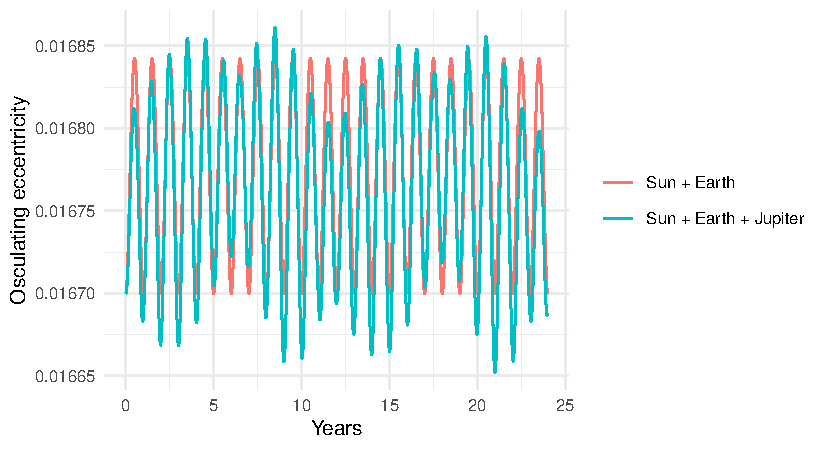
\includegraphics[width=1\linewidth,height=\textheight,keepaspectratio]{07-keplerian-elements_files/figure-pdf/fig-osculating-e-1.pdf}

}

\caption{\label{fig-osculating-e}Earth's osculating eccentricity over 24
years, alone (flat line) and with Jupiter in the system. The wiggles
repeat each time Jupiter laps Earth, every 1.09 years, on top of a
slower drift.}

\end{figure}%

The changes are small, of order \(10^{-4}\), and they are real:
Jupiter's pull on Earth is a few parts in \(10^{5}\) of the Sun's, and
over the long term it drives a slow oscillation of Earth's eccentricity
with a period of about 100,000 years that is one of the Milankovitch
cycles behind the ice ages. A 24-year run shows only the fast part. The
two-body description does not fail here; it just stops being exact, and
the elements become a \emph{description} of the motion rather than a
prediction of it. The package's \texttt{add\_planet()} elements are the
osculating elements at J2000, and the simulation takes it from there.

\begin{tcolorbox}[enhanced jigsaw, arc=.35mm, bottomrule=.15mm, bottomtitle=1mm, breakable, colback=white, colbacktitle=quarto-callout-tip-color!10!white, colframe=quarto-callout-tip-color-frame, coltitle=black, left=2mm, leftrule=.75mm, opacityback=0, opacitybacktitle=0.6, rightrule=.15mm, title={Key results}, titlerule=0mm, toprule=.15mm, toptitle=1mm]

\begin{itemize}
\tightlist
\item
  Perifocal position: \(r = a(1-e^2)/(1+e\cos\nu)\),
  \((r\cos\nu, r\sin\nu)\). Perifocal velocity:
  \((\mu/h)(-\sin\nu,\ e + \cos\nu)\) with \(h = \sqrt{\mu a(1-e^2)}\).
\item
  Inertial state: \(R_z(\Omega)R_x(i)R_z(\omega)\) applied to both, plus
  the parent's state.
\item
  Inverse: \(i\) from \(\mathbf{h}\), \(\Omega\) from
  \(\hat{\mathbf z}\times\mathbf{h}\), \(\omega\) and \(\nu\) from
  \(\mathbf{e}\), \(a\) from vis-viva.
\item
  Time to position: \(M = \sqrt{\mu/a^3}\,(t-t_p)\), solve
  \(M = E - e\sin E\), then
  \(\tan(\nu/2) = \sqrt{(1+e)/(1-e)}\tan(E/2)\).
\item
  In an N-body system the elements are osculating: they describe the
  instantaneous ellipse and drift under perturbation.
\end{itemize}

\end{tcolorbox}

\part{Doing Astrophysics with orbitr}

\chapter{The Solar System from JPL Elements}\label{sec-solar-system}

Part II built the tools. Part III uses them. This chapter takes the one
system everyone knows, asks where the package's numbers for it come
from, and then uses a single long run to do three pieces of real
astronomy: verify Kepler's third law across all eight planets and weigh
the Sun with it, measure how often Earth and Mars line up, and watch the
Sun wobble under Jupiter's pull in the way that lets astronomers find
planets around other stars.

\section{One call}\label{one-call}

\begin{Shaded}
\begin{Highlighting}[]
\NormalTok{solar }\OtherTok{\textless{}{-}} \FunctionTok{load\_solar\_system}\NormalTok{(}\AttributeTok{moon =} \ConstantTok{FALSE}\NormalTok{, }\AttributeTok{pluto =} \ConstantTok{FALSE}\NormalTok{) }\SpecialCharTok{|\textgreater{}}
  \FunctionTok{simulate\_system}\NormalTok{(}\AttributeTok{time\_step =}\NormalTok{ seconds\_per\_day, }\AttributeTok{duration =}\NormalTok{ seconds\_per\_year }\SpecialCharTok{*} \DecValTok{170}\NormalTok{)}

\NormalTok{solar }\SpecialCharTok{|\textgreater{}} \FunctionTok{count}\NormalTok{(id)}
\CommentTok{\#\textgreater{} \# A tibble: 9 x 2}
\CommentTok{\#\textgreater{}   id          n}
\CommentTok{\#\textgreater{}   \textless{}chr\textgreater{}   \textless{}int\textgreater{}}
\CommentTok{\#\textgreater{} 1 Earth   62093}
\CommentTok{\#\textgreater{} 2 Jupiter 62093}
\CommentTok{\#\textgreater{} 3 Mars    62093}
\CommentTok{\#\textgreater{} 4 Mercury 62093}
\CommentTok{\#\textgreater{} 5 Neptune 62093}
\CommentTok{\#\textgreater{} 6 Saturn  62093}
\CommentTok{\#\textgreater{} 7 Sun     62093}
\CommentTok{\#\textgreater{} 8 Uranus  62093}
\CommentTok{\#\textgreater{} 9 Venus   62093}
\end{Highlighting}
\end{Shaded}

Nine bodies for 170 years at a daily step: a little over half a million
rows, which takes a minute or so (Chapter 15 explains where the time
goes). The run is long because Neptune's period is 165 years and I want
to measure it. The Moon is left out because a daily step is far too
coarse for it (Chapter 5), and Pluto because it would need another
century.

Every planet starts at perihelion, which is the package's default, so
the planets begin lined up along their individual perihelion directions
rather than where they were on any real date. Chapter 7 showed how to
fix that with Kepler's equation if you need to; for the measurements
below it does not matter.

\section{Where the numbers come from}\label{where-the-numbers-come-from}

The elements behind \texttt{add\_planet()} are from JPL's DE440
planetary ephemeris (Park et al. 2021). An ephemeris is not a theory; it
is a fit. JPL integrates the full equations of motion of the solar
system, including general relativity, the oblateness of the Sun and
planets, hundreds of asteroids, and the Moon's own rotation, and adjusts
the initial conditions and masses until the model matches every
observation they have: centuries of optical astrometry, decades of radar
ranging to the inner planets, laser ranging to the Moon, and tracking
data from every spacecraft that has flown past or orbited a planet. The
result is positions good to well under a kilometer for the inner
planets, and the masses in Appendix~\ref{sec-constants} are by-products
of the same fit.

What the package takes from DE440 is the \emph{osculating} elements of
each planet at one instant, the J2000 epoch (noon on January 1, 2000, in
Terrestrial Time), in the ecliptic frame of that date. Those elements
describe the ellipse each planet was on at that instant. From there
orbitr integrates point-mass Newtonian gravity, nothing else. Over the
years and decades the planets' orbits stay very close to the real ones;
over centuries the effects JPL includes and orbitr does not (relativity
for Mercury, the asteroids for Mars) accumulate to differences you could
detect with a telescope but not by eye.

\section{Kepler's third law, verified}\label{keplers-third-law-verified}

Chapter 4 derived \(T = 2\pi\sqrt{a^3/\mu}\) for one planet. Kepler's
version, that \(T^2/a^3\) is the same for all planets, is the statement
that \(\mu\) is the same for all of them, which it is to the extent that
every planet's mass is negligible against the Sun's. Let's measure it.
For each planet, the osculating elements at the start give \(a\), and
\texttt{measure\_period()} gives \(T\):

\begin{Shaded}
\begin{Highlighting}[]
\NormalTok{planets }\OtherTok{\textless{}{-}} \FunctionTok{c}\NormalTok{(}\StringTok{"Mercury"}\NormalTok{, }\StringTok{"Venus"}\NormalTok{, }\StringTok{"Earth"}\NormalTok{, }\StringTok{"Mars"}\NormalTok{,}
             \StringTok{"Jupiter"}\NormalTok{, }\StringTok{"Saturn"}\NormalTok{, }\StringTok{"Uranus"}\NormalTok{, }\StringTok{"Neptune"}\NormalTok{)}

\NormalTok{kepler3 }\OtherTok{\textless{}{-}} \FunctionTok{bind\_rows}\NormalTok{(}\FunctionTok{lapply}\NormalTok{(planets, }\ControlFlowTok{function}\NormalTok{(p) \{}
  \FunctionTok{get\_orbital\_elements}\NormalTok{(solar, p, }\StringTok{"Sun"}\NormalTok{, }\AttributeTok{mu =}\NormalTok{ gravitational\_constant }\SpecialCharTok{*}\NormalTok{ mass\_sun)[}\DecValTok{1}\NormalTok{, ] }\SpecialCharTok{|\textgreater{}}
    \FunctionTok{mutate}\NormalTok{(}\AttributeTok{planet =}\NormalTok{ p,}
           \AttributeTok{T\_days =} \FunctionTok{measure\_period}\NormalTok{(solar, p, }\StringTok{"Sun"}\NormalTok{) }\SpecialCharTok{/}\NormalTok{ seconds\_per\_day)}
\NormalTok{\})) }\SpecialCharTok{|\textgreater{}}
  \FunctionTok{select}\NormalTok{(planet, a, e, T\_days)}

\NormalTok{kepler3}
\CommentTok{\#\textgreater{} \# A tibble: 8 x 4}
\CommentTok{\#\textgreater{}   planet        a       e  T\_days}
\CommentTok{\#\textgreater{}   \textless{}chr\textgreater{}     \textless{}dbl\textgreater{}   \textless{}dbl\textgreater{}   \textless{}dbl\textgreater{}}
\CommentTok{\#\textgreater{} 1 Mercury 5.79e10 0.206      88.2}
\CommentTok{\#\textgreater{} 2 Venus   1.08e11 0.00680   225. }
\CommentTok{\#\textgreater{} 3 Earth   1.50e11 0.0167    365. }
\CommentTok{\#\textgreater{} 4 Mars    2.28e11 0.0934    687. }
\CommentTok{\#\textgreater{} 5 Jupiter 7.78e11 0.0489   4329. }
\CommentTok{\#\textgreater{} 6 Saturn  1.43e12 0.0565  10786. }
\CommentTok{\#\textgreater{} 7 Uranus  2.87e12 0.0457  30795. }
\CommentTok{\#\textgreater{} 8 Neptune 4.49e12 0.0113  59514.}
\end{Highlighting}
\end{Shaded}

Mercury's 88 days and Neptune's 165 years come out of the same run. On a
log-log plot, \(T\) against \(a\) should be a straight line of slope
\(3/2\):

\begin{Shaded}
\begin{Highlighting}[]
\NormalTok{fit }\OtherTok{\textless{}{-}} \FunctionTok{lm}\NormalTok{(}\FunctionTok{log}\NormalTok{(T\_days) }\SpecialCharTok{\textasciitilde{}} \FunctionTok{log}\NormalTok{(a), }\AttributeTok{data =}\NormalTok{ kepler3)}

\NormalTok{kepler3 }\SpecialCharTok{|\textgreater{}}
  \FunctionTok{ggplot}\NormalTok{(}\FunctionTok{aes}\NormalTok{(a }\SpecialCharTok{/}\NormalTok{ distance\_earth\_sun, T\_days }\SpecialCharTok{/} \FloatTok{365.25}\NormalTok{)) }\SpecialCharTok{+}
  \FunctionTok{geom\_abline}\NormalTok{(}\AttributeTok{intercept =} \DecValTok{0}\NormalTok{, }\AttributeTok{slope =} \FloatTok{1.5}\NormalTok{, }\AttributeTok{color =} \StringTok{"grey60"}\NormalTok{) }\SpecialCharTok{+}   \CommentTok{\# T = a\^{}(3/2) in AU and years}
  \FunctionTok{geom\_point}\NormalTok{() }\SpecialCharTok{+}
  \FunctionTok{geom\_text}\NormalTok{(}\FunctionTok{aes}\NormalTok{(}\AttributeTok{label =}\NormalTok{ planet), }\AttributeTok{hjust =} \SpecialCharTok{{-}}\FloatTok{0.2}\NormalTok{, }\AttributeTok{vjust =} \FloatTok{0.3}\NormalTok{, }\AttributeTok{size =} \DecValTok{3}\NormalTok{) }\SpecialCharTok{+}
  \FunctionTok{scale\_x\_log10}\NormalTok{() }\SpecialCharTok{+} \FunctionTok{scale\_y\_log10}\NormalTok{() }\SpecialCharTok{+}
  \FunctionTok{labs}\NormalTok{(}\AttributeTok{x =} \StringTok{"Semi{-}major axis (AU)"}\NormalTok{, }\AttributeTok{y =} \StringTok{"Period (years)"}\NormalTok{)}
\end{Highlighting}
\end{Shaded}

\begin{figure}[tbp]

\centering{

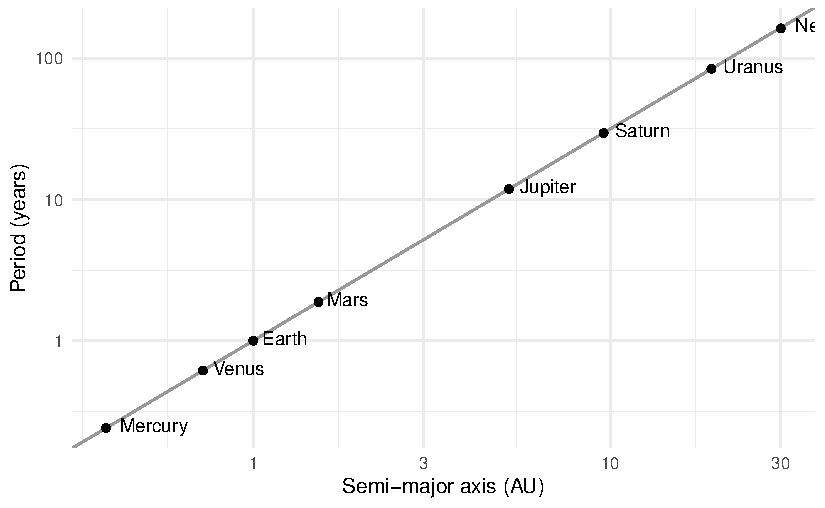
\includegraphics[width=1\linewidth,height=\textheight,keepaspectratio]{08-the-solar-system_files/figure-pdf/fig-kepler3-1.pdf}

}

\caption{\label{fig-kepler3}Orbital period against semi-major axis for
the eight planets, from the simulation. The line has slope exactly
\(3/2\).}

\end{figure}%

\begin{Shaded}
\begin{Highlighting}[]
\FunctionTok{coef}\NormalTok{(fit)[[}\StringTok{"log(a)"}\NormalTok{]]}
\CommentTok{\#\textgreater{} [1] 1.498288}
\end{Highlighting}
\end{Shaded}

That is the exponent. Now the constant. Rearranging,
\(\mu = 4\pi^2 a^3/T^2\), and \(\mu/G\) is a mass:

\begin{Shaded}
\begin{Highlighting}[]
\NormalTok{kepler3 }\SpecialCharTok{|\textgreater{}}
  \FunctionTok{mutate}\NormalTok{(}\AttributeTok{M\_implied =} \DecValTok{4} \SpecialCharTok{*}\NormalTok{ pi}\SpecialCharTok{\^{}}\DecValTok{2} \SpecialCharTok{*}\NormalTok{ a}\SpecialCharTok{\^{}}\DecValTok{3} \SpecialCharTok{/}\NormalTok{ (T\_days }\SpecialCharTok{*}\NormalTok{ seconds\_per\_day)}\SpecialCharTok{\^{}}\DecValTok{2} \SpecialCharTok{/}
\NormalTok{                     gravitational\_constant,}
         \AttributeTok{M\_over\_sun =}\NormalTok{ M\_implied }\SpecialCharTok{/}\NormalTok{ mass\_sun) }\SpecialCharTok{|\textgreater{}}
  \FunctionTok{select}\NormalTok{(planet, M\_over\_sun)}
\CommentTok{\#\textgreater{} \# A tibble: 8 x 2}
\CommentTok{\#\textgreater{}   planet  M\_over\_sun}
\CommentTok{\#\textgreater{}   \textless{}chr\textgreater{}        \textless{}dbl\textgreater{}}
\CommentTok{\#\textgreater{} 1 Mercury      0.994}
\CommentTok{\#\textgreater{} 2 Venus        0.999}
\CommentTok{\#\textgreater{} 3 Earth        1.000}
\CommentTok{\#\textgreater{} 4 Mars         1.000}
\CommentTok{\#\textgreater{} 5 Jupiter      1.00 }
\CommentTok{\#\textgreater{} 6 Saturn       1.01 }
\CommentTok{\#\textgreater{} 7 Uranus       0.994}
\CommentTok{\#\textgreater{} 8 Neptune      1.02}
\end{Highlighting}
\end{Shaded}

Every planet weighs the Sun. The answers agree to better than a part in
a thousand, and the one that disagrees most is Jupiter, because what the
period really measures is \(M_\odot + m_{\mathrm{planet}}\), and Jupiter
is a thousandth of a solar mass. Kepler had no way to know that his
third law was slightly different for each planet; the differences were
far below the precision of Tycho's data. We can see them in a table.

\begin{tcolorbox}[enhanced jigsaw, arc=.35mm, bottomrule=.15mm, bottomtitle=1mm, breakable, colback=white, colbacktitle=quarto-callout-note-color!10!white, colframe=quarto-callout-note-color-frame, coltitle=black, left=2mm, leftrule=.75mm, opacityback=0, opacitybacktitle=0.6, rightrule=.15mm, title={Where it comes from}, titlerule=0mm, toprule=.15mm, toptitle=1mm]

This is exactly how the masses in Appendix~\ref{sec-constants} were
determined, with one twist. For a planet with moons, you watch a moon:
its period and distance give
\(G(M_{\mathrm{planet}} + m_{\mathrm{moon}})\) directly. Jupiter's mass
was known to a fraction of a percent by the 18th century from the
Galilean moons, long before anyone had a good value of \(G\), which is
why astronomers habitually quote \(GM\) rather than \(M\). For Mercury
and Venus, which have no moons, the mass had to wait for spacecraft: the
bending of a spacecraft's path during a flyby is a two-body hyperbola,
and Chapter 4's formulas give the mass from the deflection.

\end{tcolorbox}

\section{How often do Earth and Mars line
up?}\label{how-often-do-earth-and-mars-line-up}

Mars is closest to Earth, and brightest in our sky, at
\emph{opposition}, when Earth passes between Mars and the Sun, so that
the two planets have the same heliocentric longitude. How often does
that happen? Earth laps Mars, and the time between lappings, the
\emph{synodic period}, follows from the angular rates. Earth's longitude
advances at \(2\pi/T_E\) per unit time and Mars's at \(2\pi/T_M\), so
the difference advances at \(2\pi(1/T_E - 1/T_M)\), and one full lap
takes

\begin{equation}\protect\phantomsection\label{eq-synodic}{
\frac{1}{T_{\mathrm{syn}}} = \frac{1}{T_E} - \frac{1}{T_M}.
}\end{equation}

With the measured periods:

\begin{Shaded}
\begin{Highlighting}[]
\NormalTok{T\_E }\OtherTok{\textless{}{-}}\NormalTok{ kepler3}\SpecialCharTok{$}\NormalTok{T\_days[kepler3}\SpecialCharTok{$}\NormalTok{planet }\SpecialCharTok{==} \StringTok{"Earth"}\NormalTok{]}
\NormalTok{T\_M }\OtherTok{\textless{}{-}}\NormalTok{ kepler3}\SpecialCharTok{$}\NormalTok{T\_days[kepler3}\SpecialCharTok{$}\NormalTok{planet }\SpecialCharTok{==} \StringTok{"Mars"}\NormalTok{]}
\DecValTok{1} \SpecialCharTok{/}\NormalTok{ (}\DecValTok{1} \SpecialCharTok{/}\NormalTok{ T\_E }\SpecialCharTok{{-}} \DecValTok{1} \SpecialCharTok{/}\NormalTok{ T\_M)}
\CommentTok{\#\textgreater{} [1] 780.2493}
\end{Highlighting}
\end{Shaded}

About 780 days, or two years and seven weeks. Now from the data
directly. Compute each planet's heliocentric longitude, unwrap it so it
grows continuously, and take the difference:

\begin{Shaded}
\begin{Highlighting}[]
\NormalTok{longitude }\OtherTok{\textless{}{-}} \ControlFlowTok{function}\NormalTok{(sim, body) \{}
  \FunctionTok{relative\_state}\NormalTok{(sim, body, }\StringTok{"Sun"}\NormalTok{) }\SpecialCharTok{|\textgreater{}}
    \FunctionTok{transmute}\NormalTok{(time, }\AttributeTok{lambda =} \FunctionTok{unwrap}\NormalTok{(}\FunctionTok{atan2}\NormalTok{(ry, rx)))}
\NormalTok{\}}

\NormalTok{lap }\OtherTok{\textless{}{-}} \FunctionTok{inner\_join}\NormalTok{(}\FunctionTok{longitude}\NormalTok{(solar, }\StringTok{"Earth"}\NormalTok{), }\FunctionTok{longitude}\NormalTok{(solar, }\StringTok{"Mars"}\NormalTok{),}
                  \AttributeTok{by =} \StringTok{"time"}\NormalTok{, }\AttributeTok{suffix =} \FunctionTok{c}\NormalTok{(}\StringTok{"\_earth"}\NormalTok{, }\StringTok{"\_mars"}\NormalTok{)) }\SpecialCharTok{|\textgreater{}}
  \FunctionTok{mutate}\NormalTok{(}\AttributeTok{lead =}\NormalTok{ lambda\_earth }\SpecialCharTok{{-}}\NormalTok{ lambda\_mars)}
\end{Highlighting}
\end{Shaded}

The lead grows by \(2\pi\) per synodic period, so its average slope
gives \(T_{\mathrm{syn}}\) directly:

\begin{Shaded}
\begin{Highlighting}[]
\NormalTok{slope }\OtherTok{\textless{}{-}} \FunctionTok{coef}\NormalTok{(}\FunctionTok{lm}\NormalTok{(lead }\SpecialCharTok{\textasciitilde{}}\NormalTok{ time, }\AttributeTok{data =}\NormalTok{ lap))[[}\StringTok{"time"}\NormalTok{]]}
\DecValTok{2} \SpecialCharTok{*}\NormalTok{ pi }\SpecialCharTok{/}\NormalTok{ slope }\SpecialCharTok{/}\NormalTok{ seconds\_per\_day}
\CommentTok{\#\textgreater{} [1] 780.2043}
\end{Highlighting}
\end{Shaded}

The two agree. But the lead does not grow uniformly. The times when it
passes a multiple of \(2\pi\) are the oppositions:

\begin{Shaded}
\begin{Highlighting}[]
\NormalTok{oppositions }\OtherTok{\textless{}{-}}\NormalTok{ lap }\SpecialCharTok{|\textgreater{}}
  \FunctionTok{filter}\NormalTok{(}\FunctionTok{floor}\NormalTok{(lead }\SpecialCharTok{/}\NormalTok{ (}\DecValTok{2} \SpecialCharTok{*}\NormalTok{ pi)) }\SpecialCharTok{!=} \FunctionTok{lag}\NormalTok{(}\FunctionTok{floor}\NormalTok{(lead }\SpecialCharTok{/}\NormalTok{ (}\DecValTok{2} \SpecialCharTok{*}\NormalTok{ pi)))) }\SpecialCharTok{|\textgreater{}}
  \FunctionTok{pull}\NormalTok{(time) }\SpecialCharTok{/}\NormalTok{ seconds\_per\_day}

\FunctionTok{head}\NormalTok{(}\FunctionTok{diff}\NormalTok{(oppositions), }\DecValTok{8}\NormalTok{)}
\CommentTok{\#\textgreater{} [1] 783 809 799 775 767 764 767 777}
\end{Highlighting}
\end{Shaded}

The gaps between successive oppositions swing from about 764 to 810
days. The reason is Mars's eccentricity: it moves faster near perihelion
and slower near aphelion, so Earth catches it sooner or later depending
on where in its orbit the catching happens. Oppositions near Mars's
perihelion are also the close ones, when Mars is at its largest and
brightest in our sky; they recur every 15 to 17 years, and the synodic
period alone does not tell you that. The simulation does.

\section{The Sun wobbles}\label{the-sun-wobbles}

The Sun is not fixed. Chapter 4's center-of-mass analysis applies to
every pair, and Jupiter, a thousandth of a solar mass at 5.2 AU, pulls
the Sun around a circle of radius about 0.005 AU, a little more than the
Sun's own radius, once every 11.9 years. The Sun's speed on that circle
is a dozen meters per second. That number is the foundation of the
radial-velocity method for finding planets around other stars: you
cannot see the planet, but a spectrograph can see the star's velocity
along your line of sight change by meters per second as the planet goes
around.

\texttt{load\_solar\_system()} starts the Sun at rest at the origin, so
the system's center of mass drifts slowly (Chapter 2 again). To see the
wobble alone, look at the Sun in the barycentric frame, where the center
of mass is at rest by construction:

\begin{Shaded}
\begin{Highlighting}[]
\NormalTok{sun\_wobble }\OtherTok{\textless{}{-}}\NormalTok{ solar }\SpecialCharTok{|\textgreater{}}
  \FunctionTok{shift\_reference\_frame}\NormalTok{(}\StringTok{"barycenter"}\NormalTok{) }\SpecialCharTok{|\textgreater{}}
  \FunctionTok{filter}\NormalTok{(id }\SpecialCharTok{==} \StringTok{"Sun"}\NormalTok{)}
\end{Highlighting}
\end{Shaded}

\begin{Shaded}
\begin{Highlighting}[]
\NormalTok{sun\_wobble }\SpecialCharTok{|\textgreater{}}
  \FunctionTok{filter}\NormalTok{(time }\SpecialCharTok{\textless{}}\NormalTok{ seconds\_per\_year }\SpecialCharTok{*} \DecValTok{60}\NormalTok{) }\SpecialCharTok{|\textgreater{}}
  \FunctionTok{ggplot}\NormalTok{(}\FunctionTok{aes}\NormalTok{(time }\SpecialCharTok{/}\NormalTok{ seconds\_per\_year, vx)) }\SpecialCharTok{+}
  \FunctionTok{geom\_line}\NormalTok{() }\SpecialCharTok{+}
  \FunctionTok{labs}\NormalTok{(}\AttributeTok{x =} \StringTok{"Years"}\NormalTok{, }\AttributeTok{y =} \StringTok{"Sun\textquotesingle{}s velocity, x component (m/s)"}\NormalTok{)}
\end{Highlighting}
\end{Shaded}

\begin{figure}[tbp]

\centering{

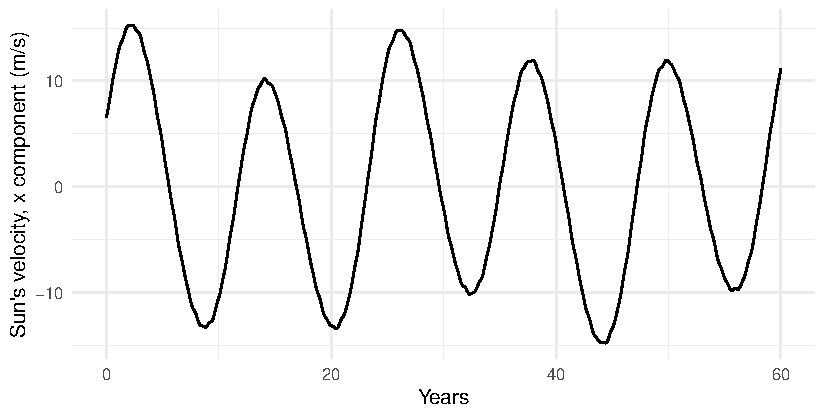
\includegraphics[width=1\linewidth,height=\textheight,keepaspectratio]{08-the-solar-system_files/figure-pdf/fig-sun-wobble-1.pdf}

}

\caption{\label{fig-sun-wobble}The Sun's velocity relative to the solar
system's center of mass, \(x\) component, over 60 years. The 12-year, 12
m/s oscillation is Jupiter; the slower modulation on top of it is
Saturn.}

\end{figure}%

Twelve meters per second is a brisk walking pace, measured on a star.
For a distant observer sitting in the plane of the solar system, that is
the signal the Sun would show. Modern spectrographs reach below one
meter per second, which is enough to find Saturn (about 3 m/s) and, with
patience, Neptune. Earth's contribution is nine centimeters per second,
which is why finding true Earth twins this way is still at the edge of
what is possible.

\section{A long run checked}\label{a-long-run-checked}

A 170-year integration is long enough that it is worth asking whether
the integrator held up. The total energy of a nine-body system needs
every pair at every time step, which for 62,000 steps and 36 pairs is
more rows than we need; sampling every 30 days is plenty for a drift
check:

\begin{Shaded}
\begin{Highlighting}[]
\NormalTok{solar }\SpecialCharTok{|\textgreater{}}
  \FunctionTok{filter}\NormalTok{(time }\SpecialCharTok{\%\%}\NormalTok{ (seconds\_per\_day }\SpecialCharTok{*} \DecValTok{30}\NormalTok{) }\SpecialCharTok{==} \DecValTok{0}\NormalTok{) }\SpecialCharTok{|\textgreater{}}
  \FunctionTok{conserved\_quantities}\NormalTok{() }\SpecialCharTok{|\textgreater{}}
  \FunctionTok{ggplot}\NormalTok{(}\FunctionTok{aes}\NormalTok{(time }\SpecialCharTok{/}\NormalTok{ seconds\_per\_year, energy\_error)) }\SpecialCharTok{+}
  \FunctionTok{geom\_line}\NormalTok{() }\SpecialCharTok{+}
  \FunctionTok{labs}\NormalTok{(}\AttributeTok{x =} \StringTok{"Years"}\NormalTok{, }\AttributeTok{y =} \StringTok{"Relative energy error"}\NormalTok{)}
\end{Highlighting}
\end{Shaded}

\begin{figure}[tbp]

\centering{

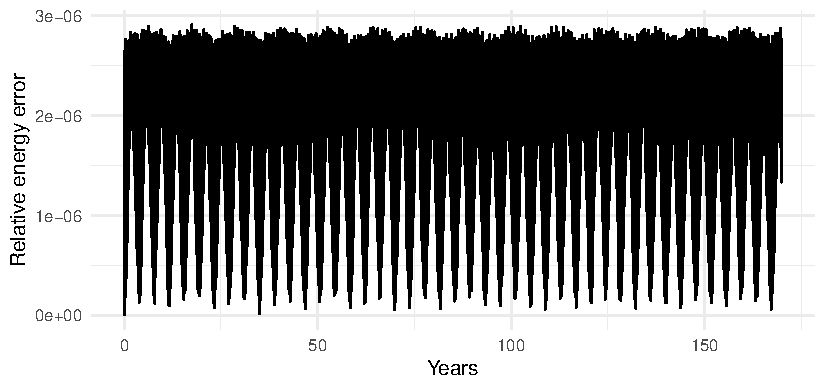
\includegraphics[width=1\linewidth,height=\textheight,keepaspectratio]{08-the-solar-system_files/figure-pdf/fig-solar-energy-1.pdf}

}

\caption{\label{fig-solar-energy}Relative energy error of the 170-year
solar system run, sampled every 30 days. The oscillation is Mercury's
orbit; there is no drift.}

\end{figure}%

The error oscillates at the level set by Mercury, the tightest orbit,
and does not grow, which is Chapter 5's promise kept over 62,000 steps.
If you double the duration, the band stays the same width. If you double
the step, it gets four times wider. Both are worth doing once to see.

\begin{tcolorbox}[enhanced jigsaw, arc=.35mm, bottomrule=.15mm, bottomtitle=1mm, breakable, colback=white, colbacktitle=quarto-callout-tip-color!10!white, colframe=quarto-callout-tip-color-frame, coltitle=black, left=2mm, leftrule=.75mm, opacityback=0, opacitybacktitle=0.6, rightrule=.15mm, title={Key results}, titlerule=0mm, toprule=.15mm, toptitle=1mm]

\begin{itemize}
\tightlist
\item
  The package's planets are osculating J2000 elements from JPL DE440,
  integrated with Newtonian point-mass gravity.
\item
  Kepler's third law holds across all eight planets to better than a
  part in a thousand; the residual is each planet's own mass.
\item
  Synodic period: \(1/T_{\mathrm{syn}} = 1/T_1 - 1/T_2\). Earth-Mars:
  about 780 days, varying by \(\pm 3\%\) because of Mars's eccentricity.
\item
  The Sun moves at about 12 m/s because of Jupiter; this is the
  radial-velocity exoplanet signal.
\end{itemize}

\end{tcolorbox}

\chapter{Binary Stars and Circumbinary Planets}\label{sec-binary-stars}

Most stars are not alone. Roughly half of Sun-like stars have a
companion, and the ``central body at rest at the origin'' picture that
works for the solar system fails completely for a pair of comparable
masses: both stars move, both move a lot, and the only thing that stays
put is the point between them. The Kepler-16 example in the package
documentation sets up a real binary with a planet around it, using four
velocity formulas stated without derivation. This chapter derives them
from Chapter 4, checks each one against the simulation, extends them to
an eccentric binary, and then asks the question the discoverers of
Kepler-16b had to answer: how close to a pair of stars can a planet
orbit and survive?

\section{Two stars}\label{two-stars}

Take stars of mass \(m_A\) and \(m_B\) a distance \(d\) apart on
circular orbits. Chapter 4 reduced this to a single relative orbit with
gravitational parameter \(\mu = G(m_A + m_B)\), so the relative speed on
a circle of radius \(d\) is \(u = \sqrt{G(m_A+m_B)/d}\). Each star's
actual orbit is around the center of mass, and from
Equation~\ref{eq-individual} the two stars sit on opposite sides of it
at distances

\begin{equation}\protect\phantomsection\label{eq-binary-radii}{
r_A = \frac{m_B}{m_A + m_B}\,d, \qquad r_B = \frac{m_A}{m_A + m_B}\,d,
}\end{equation}

so the heavier star makes the smaller circle. The speeds scale the same
way, \(v_A = u\,m_B/(m_A+m_B)\) and \(v_B = u\,m_A/(m_A+m_B)\), and
substituting \(u\):

\begin{equation}\protect\phantomsection\label{eq-binary-speeds}{
v_A = \sqrt{\frac{G\,m_B^2}{(m_A + m_B)\,d}}, \qquad
v_B = \sqrt{\frac{G\,m_A^2}{(m_A + m_B)\,d}}.
}\end{equation}

These are the formulas in the documentation. Note what they say: the
star you are computing the speed \emph{of} appears only in the
denominator, inside the total mass; the numerator has the mass of the
\emph{other} star. A light companion barely moves the heavy primary. The
momenta \(m_A v_A\) and \(m_B v_B\) are equal, so with the stars on
opposite sides moving in opposite directions, the total momentum is zero
and the center of mass stays at the origin. The period, from Kepler's
third law with \(a = d\), is \(T = 2\pi\sqrt{d^3/G(m_A+m_B)}\) for both
stars; they must have the same period, since they are always opposite
each other.

A function that builds any circular binary from these formulas:

\begin{Shaded}
\begin{Highlighting}[]
\NormalTok{add\_binary }\OtherTok{\textless{}{-}} \ControlFlowTok{function}\NormalTok{(system, m\_A, m\_B, d, }\AttributeTok{ids =} \FunctionTok{c}\NormalTok{(}\StringTok{"A"}\NormalTok{, }\StringTok{"B"}\NormalTok{)) \{}
\NormalTok{  r\_A }\OtherTok{\textless{}{-}}\NormalTok{ d }\SpecialCharTok{*}\NormalTok{ m\_B }\SpecialCharTok{/}\NormalTok{ (m\_A }\SpecialCharTok{+}\NormalTok{ m\_B)}
\NormalTok{  r\_B }\OtherTok{\textless{}{-}}\NormalTok{ d }\SpecialCharTok{*}\NormalTok{ m\_A }\SpecialCharTok{/}\NormalTok{ (m\_A }\SpecialCharTok{+}\NormalTok{ m\_B)}
\NormalTok{  v\_A }\OtherTok{\textless{}{-}} \FunctionTok{sqrt}\NormalTok{(gravitational\_constant }\SpecialCharTok{*}\NormalTok{ m\_B}\SpecialCharTok{\^{}}\DecValTok{2} \SpecialCharTok{/}\NormalTok{ ((m\_A }\SpecialCharTok{+}\NormalTok{ m\_B) }\SpecialCharTok{*}\NormalTok{ d))}
\NormalTok{  v\_B }\OtherTok{\textless{}{-}} \FunctionTok{sqrt}\NormalTok{(gravitational\_constant }\SpecialCharTok{*}\NormalTok{ m\_A}\SpecialCharTok{\^{}}\DecValTok{2} \SpecialCharTok{/}\NormalTok{ ((m\_A }\SpecialCharTok{+}\NormalTok{ m\_B) }\SpecialCharTok{*}\NormalTok{ d))}
\NormalTok{  system }\SpecialCharTok{|\textgreater{}}
    \FunctionTok{add\_body}\NormalTok{(ids[}\DecValTok{1}\NormalTok{], }\AttributeTok{mass =}\NormalTok{ m\_A, }\AttributeTok{x =}\NormalTok{  r\_A, }\AttributeTok{vy =}\NormalTok{  v\_A) }\SpecialCharTok{|\textgreater{}}
    \FunctionTok{add\_body}\NormalTok{(ids[}\DecValTok{2}\NormalTok{], }\AttributeTok{mass =}\NormalTok{ m\_B, }\AttributeTok{x =} \SpecialCharTok{{-}}\NormalTok{r\_B, }\AttributeTok{vy =} \SpecialCharTok{{-}}\NormalTok{v\_B)}
\NormalTok{\}}
\end{Highlighting}
\end{Shaded}

Check it on a lopsided pair, a Sun-mass star with a companion of a tenth
of the mass, one AU apart:

\begin{Shaded}
\begin{Highlighting}[]
\NormalTok{pair }\OtherTok{\textless{}{-}} \FunctionTok{create\_system}\NormalTok{() }\SpecialCharTok{|\textgreater{}}
  \FunctionTok{add\_binary}\NormalTok{(}\AttributeTok{m\_A =}\NormalTok{ mass\_sun, }\AttributeTok{m\_B =} \FloatTok{0.1} \SpecialCharTok{*}\NormalTok{ mass\_sun, }\AttributeTok{d =}\NormalTok{ distance\_earth\_sun) }\SpecialCharTok{|\textgreater{}}
  \FunctionTok{simulate\_system}\NormalTok{(}\AttributeTok{time\_step =}\NormalTok{ seconds\_per\_hour }\SpecialCharTok{*} \DecValTok{6}\NormalTok{, }\AttributeTok{duration =}\NormalTok{ seconds\_per\_year }\SpecialCharTok{*} \DecValTok{2}\NormalTok{)}

\NormalTok{pair }\SpecialCharTok{|\textgreater{}}
  \FunctionTok{group\_by}\NormalTok{(id) }\SpecialCharTok{|\textgreater{}}
  \FunctionTok{summarise}\NormalTok{(}\AttributeTok{r\_min\_AU =} \FunctionTok{min}\NormalTok{(}\FunctionTok{sqrt}\NormalTok{(x}\SpecialCharTok{\^{}}\DecValTok{2} \SpecialCharTok{+}\NormalTok{ y}\SpecialCharTok{\^{}}\DecValTok{2}\NormalTok{)) }\SpecialCharTok{/}\NormalTok{ distance\_earth\_sun,}
            \AttributeTok{r\_max\_AU =} \FunctionTok{max}\NormalTok{(}\FunctionTok{sqrt}\NormalTok{(x}\SpecialCharTok{\^{}}\DecValTok{2} \SpecialCharTok{+}\NormalTok{ y}\SpecialCharTok{\^{}}\DecValTok{2}\NormalTok{)) }\SpecialCharTok{/}\NormalTok{ distance\_earth\_sun)}
\CommentTok{\#\textgreater{} \# A tibble: 2 x 3}
\CommentTok{\#\textgreater{}   id    r\_min\_AU r\_max\_AU}
\CommentTok{\#\textgreater{}   \textless{}chr\textgreater{}    \textless{}dbl\textgreater{}    \textless{}dbl\textgreater{}}
\CommentTok{\#\textgreater{} 1 A       0.0909   0.0909}
\CommentTok{\#\textgreater{} 2 B       0.909    0.909}
\end{Highlighting}
\end{Shaded}

Each star stays on a circle (minimum and maximum radius agree), the
radii are in the ratio 1 to 10 as Equation~\ref{eq-binary-radii} says,
and they add to one AU. The period should be shorter than a year by the
factor \(\sqrt{1.1}\), because the total mass is \(1.1\,M_\odot\):

\begin{Shaded}
\begin{Highlighting}[]
\FunctionTok{c}\NormalTok{(}\AttributeTok{predicted =} \FloatTok{365.25} \SpecialCharTok{/} \FunctionTok{sqrt}\NormalTok{(}\FloatTok{1.1}\NormalTok{),}
  \AttributeTok{measured  =} \FunctionTok{measure\_period}\NormalTok{(pair, }\StringTok{"B"}\NormalTok{, }\StringTok{"A"}\NormalTok{) }\SpecialCharTok{/}\NormalTok{ seconds\_per\_day)}
\CommentTok{\#\textgreater{} predicted  measured }
\CommentTok{\#\textgreater{}  348.2522  348.2169}
\end{Highlighting}
\end{Shaded}

For a binary the natural frame is the one centered on the pair's center
of mass, and \texttt{shift\_reference\_frame(sim,\ "barycenter")} puts
every time step in it. In that frame the center of mass sits at the
origin at rest, and a body's distance from the origin is its distance
from the barycenter, which is what a circumbinary planet orbits.
\texttt{measure\_period()} with no \texttt{center} argument measures a
body's period about the origin, which is how the next section uses it.

\section{An eccentric binary}\label{an-eccentric-binary}

Real binaries are rarely circular. Kepler-16's two stars have
\(e = 0.16\). The same reduction handles it: pick the relative orbit,
then split it between the stars by the mass ratio. If the relative orbit
has semi-major axis \(a_{\mathrm{bin}}\) and eccentricity \(e\), start
the stars at periapsis, where the separation is
\(d_p = a_{\mathrm{bin}}(1-e)\) and the relative speed, from vis-viva,
is

\begin{equation}\protect\phantomsection\label{eq-binary-periapsis}{
u_p = \sqrt{\frac{\mu}{a_{\mathrm{bin}}}\cdot\frac{1+e}{1-e}}, \qquad \mu = G(m_A+m_B).
}\end{equation}

Then \(v_A = u_p\,m_B/(m_A+m_B)\) and \(v_B = u_p\,m_A/(m_A+m_B)\) as
before, and the stars are placed at \(d_p\,m_B/(m_A+m_B)\) and
\(d_p\,m_A/(m_A+m_B)\) on either side of the origin.

\begin{Shaded}
\begin{Highlighting}[]
\NormalTok{add\_eccentric\_binary }\OtherTok{\textless{}{-}} \ControlFlowTok{function}\NormalTok{(system, m\_A, m\_B, a\_bin, e, }\AttributeTok{ids =} \FunctionTok{c}\NormalTok{(}\StringTok{"A"}\NormalTok{, }\StringTok{"B"}\NormalTok{)) \{}
\NormalTok{  M   }\OtherTok{\textless{}{-}}\NormalTok{ m\_A }\SpecialCharTok{+}\NormalTok{ m\_B}
\NormalTok{  d\_p }\OtherTok{\textless{}{-}}\NormalTok{ a\_bin }\SpecialCharTok{*}\NormalTok{ (}\DecValTok{1} \SpecialCharTok{{-}}\NormalTok{ e)}
\NormalTok{  u\_p }\OtherTok{\textless{}{-}} \FunctionTok{sqrt}\NormalTok{(gravitational\_constant }\SpecialCharTok{*}\NormalTok{ M }\SpecialCharTok{/}\NormalTok{ a\_bin }\SpecialCharTok{*}\NormalTok{ (}\DecValTok{1} \SpecialCharTok{+}\NormalTok{ e) }\SpecialCharTok{/}\NormalTok{ (}\DecValTok{1} \SpecialCharTok{{-}}\NormalTok{ e))}
\NormalTok{  system }\SpecialCharTok{|\textgreater{}}
    \FunctionTok{add\_body}\NormalTok{(ids[}\DecValTok{1}\NormalTok{], }\AttributeTok{mass =}\NormalTok{ m\_A, }\AttributeTok{x =}\NormalTok{  d\_p }\SpecialCharTok{*}\NormalTok{ m\_B }\SpecialCharTok{/}\NormalTok{ M, }\AttributeTok{vy =}\NormalTok{  u\_p }\SpecialCharTok{*}\NormalTok{ m\_B }\SpecialCharTok{/}\NormalTok{ M) }\SpecialCharTok{|\textgreater{}}
    \FunctionTok{add\_body}\NormalTok{(ids[}\DecValTok{2}\NormalTok{], }\AttributeTok{mass =}\NormalTok{ m\_B, }\AttributeTok{x =} \SpecialCharTok{{-}}\NormalTok{d\_p }\SpecialCharTok{*}\NormalTok{ m\_A }\SpecialCharTok{/}\NormalTok{ M, }\AttributeTok{vy =} \SpecialCharTok{{-}}\NormalTok{u\_p }\SpecialCharTok{*}\NormalTok{ m\_A }\SpecialCharTok{/}\NormalTok{ M)}
\NormalTok{\}}
\end{Highlighting}
\end{Shaded}

The eccentricity vector from Chapter 4 checks that this produced the
orbit it was supposed to:

\begin{Shaded}
\begin{Highlighting}[]
\NormalTok{ecc\_pair }\OtherTok{\textless{}{-}} \FunctionTok{create\_system}\NormalTok{() }\SpecialCharTok{|\textgreater{}}
  \FunctionTok{add\_eccentric\_binary}\NormalTok{(}\AttributeTok{m\_A =}\NormalTok{ mass\_sun, }\AttributeTok{m\_B =} \FloatTok{0.5} \SpecialCharTok{*}\NormalTok{ mass\_sun,}
                       \AttributeTok{a\_bin =}\NormalTok{ distance\_earth\_sun, }\AttributeTok{e =} \FloatTok{0.4}\NormalTok{) }\SpecialCharTok{|\textgreater{}}
  \FunctionTok{simulate\_system}\NormalTok{(}\AttributeTok{time\_step =}\NormalTok{ seconds\_per\_hour }\SpecialCharTok{*} \DecValTok{6}\NormalTok{, }\AttributeTok{duration =}\NormalTok{ seconds\_per\_year)}

\FunctionTok{get\_orbital\_elements}\NormalTok{(ecc\_pair, }\StringTok{"B"}\NormalTok{, }\StringTok{"A"}\NormalTok{, }\AttributeTok{mu =}\NormalTok{ gravitational\_constant }\SpecialCharTok{*} \FloatTok{1.5} \SpecialCharTok{*}\NormalTok{ mass\_sun) }\SpecialCharTok{|\textgreater{}}
  \FunctionTok{summarise}\NormalTok{(}\AttributeTok{e\_min =} \FunctionTok{min}\NormalTok{(e), }\AttributeTok{e\_max =} \FunctionTok{max}\NormalTok{(e))}
\CommentTok{\#\textgreater{} \# A tibble: 1 x 2}
\CommentTok{\#\textgreater{}   e\_min e\_max}
\CommentTok{\#\textgreater{}   \textless{}dbl\textgreater{} \textless{}dbl\textgreater{}}
\CommentTok{\#\textgreater{} 1 0.400 0.400}
\end{Highlighting}
\end{Shaded}

\section{Kepler-16}\label{kepler-16}

Kepler-16b was the first planet confirmed to orbit two stars, found in
2011 by the Kepler spacecraft when it was seen transiting both of them
({Doyle et al.} 2011). The system is a K-type star of \(0.69\,M_\odot\)
and an M-type star of \(0.20\,M_\odot\) in a 41-day orbit with
semi-major axis 0.224 AU and eccentricity 0.16, and a Saturn-mass planet
(\(0.33\,M_{\mathrm{Jup}}\)) orbiting the pair every 229 days at 0.705
AU, on a nearly circular orbit in the same plane. The documentation
builds it with a circular binary; here it is with the real eccentricity.

The planet is far enough out that the two stars act on it almost like a
single star of their combined mass at the barycenter. So the planet goes
on a circle of radius \(0.705\) AU around the origin at the circular
speed for mass \(m_A + m_B\):

\begin{Shaded}
\begin{Highlighting}[]
\NormalTok{AU  }\OtherTok{\textless{}{-}}\NormalTok{ distance\_earth\_sun}
\NormalTok{m\_A }\OtherTok{\textless{}{-}} \FloatTok{0.69} \SpecialCharTok{*}\NormalTok{ mass\_sun}
\NormalTok{m\_B }\OtherTok{\textless{}{-}} \FloatTok{0.20} \SpecialCharTok{*}\NormalTok{ mass\_sun}
\NormalTok{m\_p }\OtherTok{\textless{}{-}} \FloatTok{0.333} \SpecialCharTok{*}\NormalTok{ mass\_jupiter}

\NormalTok{r\_planet }\OtherTok{\textless{}{-}} \FloatTok{0.7048} \SpecialCharTok{*}\NormalTok{ AU}
\NormalTok{v\_planet }\OtherTok{\textless{}{-}} \FunctionTok{sqrt}\NormalTok{(gravitational\_constant }\SpecialCharTok{*}\NormalTok{ (m\_A }\SpecialCharTok{+}\NormalTok{ m\_B) }\SpecialCharTok{/}\NormalTok{ r\_planet)}

\NormalTok{kepler16 }\OtherTok{\textless{}{-}} \FunctionTok{create\_system}\NormalTok{() }\SpecialCharTok{|\textgreater{}}
  \FunctionTok{add\_eccentric\_binary}\NormalTok{(m\_A, m\_B, }\AttributeTok{a\_bin =} \FloatTok{0.2243} \SpecialCharTok{*}\NormalTok{ AU, }\AttributeTok{e =} \FloatTok{0.159}\NormalTok{,}
                       \AttributeTok{ids =} \FunctionTok{c}\NormalTok{(}\StringTok{"Kepler{-}16A"}\NormalTok{, }\StringTok{"Kepler{-}16B"}\NormalTok{)) }\SpecialCharTok{|\textgreater{}}
  \FunctionTok{add\_body}\NormalTok{(}\StringTok{"Kepler{-}16b"}\NormalTok{, }\AttributeTok{mass =}\NormalTok{ m\_p, }\AttributeTok{x =}\NormalTok{ r\_planet, }\AttributeTok{vy =}\NormalTok{ v\_planet) }\SpecialCharTok{|\textgreater{}}
  \FunctionTok{simulate\_system}\NormalTok{(}\AttributeTok{time\_step =}\NormalTok{ seconds\_per\_hour, }\AttributeTok{duration =}\NormalTok{ seconds\_per\_year }\SpecialCharTok{*} \DecValTok{2}\NormalTok{)}
\end{Highlighting}
\end{Shaded}

\begin{Shaded}
\begin{Highlighting}[]
\FunctionTok{plot\_orbits}\NormalTok{(kepler16)}
\end{Highlighting}
\end{Shaded}

\begin{figure}[tbp]

\centering{

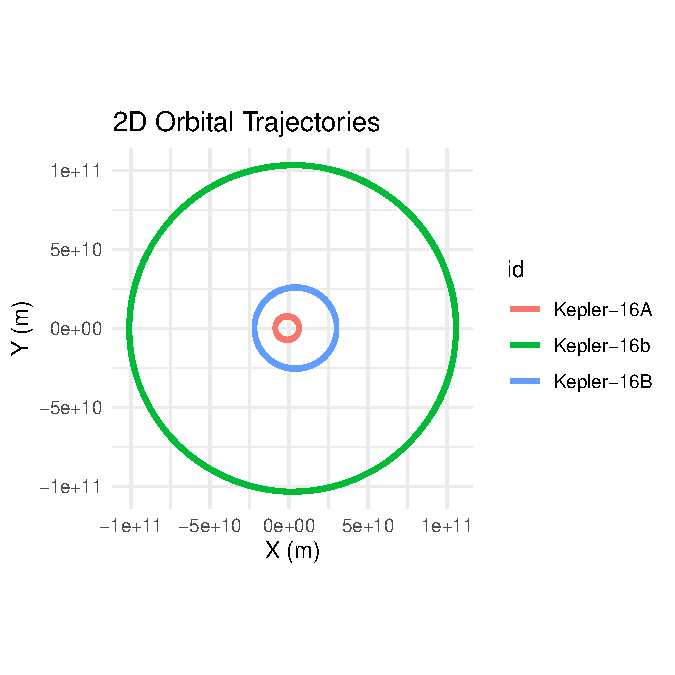
\includegraphics[width=0.7\linewidth,height=\textheight,keepaspectratio]{09-binary-stars_files/figure-pdf/fig-kepler16-1.pdf}

}

\caption{\label{fig-kepler16}Kepler-16 for two years. The two stars
orbit their common center of mass every 41 days while the planet circles
the pair every 229 days.}

\end{figure}%

The planet's orbit is not a two-body orbit about anything, but about the
barycenter it is very nearly one, and the barycentric frame lets us
measure it. The predictions are Kepler's third law with the
\emph{combined} mass of all three bodies, and a period of 229 days for
the planet and 41 days for the stars:

\begin{Shaded}
\begin{Highlighting}[]
\NormalTok{k16 }\OtherTok{\textless{}{-}} \FunctionTok{shift\_reference\_frame}\NormalTok{(kepler16, }\StringTok{"barycenter"}\NormalTok{)}
\NormalTok{mu\_total }\OtherTok{\textless{}{-}}\NormalTok{ gravitational\_constant }\SpecialCharTok{*}\NormalTok{ (m\_A }\SpecialCharTok{+}\NormalTok{ m\_B }\SpecialCharTok{+}\NormalTok{ m\_p)}

\FunctionTok{c}\NormalTok{(}\AttributeTok{planet\_predicted\_days =} \DecValTok{2} \SpecialCharTok{*}\NormalTok{ pi }\SpecialCharTok{*} \FunctionTok{sqrt}\NormalTok{(r\_planet}\SpecialCharTok{\^{}}\DecValTok{3} \SpecialCharTok{/}\NormalTok{ mu\_total) }\SpecialCharTok{/}\NormalTok{ seconds\_per\_day,}
  \AttributeTok{planet\_measured\_days  =} \FunctionTok{measure\_period}\NormalTok{(k16, }\StringTok{"Kepler{-}16b"}\NormalTok{) }\SpecialCharTok{/}\NormalTok{ seconds\_per\_day,}
  \AttributeTok{binary\_measured\_days  =} \FunctionTok{measure\_period}\NormalTok{(k16, }\StringTok{"Kepler{-}16B"}\NormalTok{, }\StringTok{"Kepler{-}16A"}\NormalTok{) }\SpecialCharTok{/}
\NormalTok{                          seconds\_per\_day)}
\CommentTok{\#\textgreater{} planet\_predicted\_days  planet\_measured\_days  binary\_measured\_days }
\CommentTok{\#\textgreater{}             229.01798             220.79718              41.12564}
\end{Highlighting}
\end{Shaded}

Both match the published periods. The planet is not \emph{exactly} on a
circle, because the two stars' pull is not exactly that of a point at
the barycenter; the difference is a small periodic wobble at the
binary's period, and you can see it by plotting the planet's distance
from the barycenter over time. That wobble is real and it is how the
planet's orbit was characterized from the transit timing.

\begin{tcolorbox}[enhanced jigsaw, arc=.35mm, bottomrule=.15mm, bottomtitle=1mm, breakable, colback=white, colbacktitle=quarto-callout-note-color!10!white, colframe=quarto-callout-note-color-frame, coltitle=black, left=2mm, leftrule=.75mm, opacityback=0, opacitybacktitle=0.6, rightrule=.15mm, title={Where it comes from}, titlerule=0mm, toprule=.15mm, toptitle=1mm]

The transit method finds planets by the dip in a star's brightness when
the planet crosses in front of it. For Kepler-16 the light curve showed
the planet crossing \emph{both} stars, and the two stars eclipsing each
other, so the geometry of the whole system could be reconstructed from
timing alone. The paper includes a diagram of the three orbits that
looks almost exactly like Figure~\ref{fig-kepler16}. Working out the
masses needed a full three-body fit, because the planet's orbit is
noticeably non-Keplerian: the stars' motion makes the planet's transit
times and durations vary noticeably from one transit to the next, and
the size of the variation fixes the mass ratio.

\end{tcolorbox}

\section{How close is too close?}\label{how-close-is-too-close}

A planet orbiting a binary can only survive if it is far enough out that
the two stars act like one. Too close, and the alternating pulls of the
stars as they go around pump energy into the planet's orbit until it is
ejected or thrown into one of the stars. The boundary is not sharp, and
it depends on the binary's mass ratio and eccentricity, but it is
roughly two to four times the binary's separation. Holman and Wiegert
(Holman and Wiegert 1999) ran thousands of three-body simulations and
fitted a formula for the critical semi-major axis:

\begin{equation}\protect\phantomsection\label{eq-holman-wiegert}{
\frac{a_{\mathrm{crit}}}{a_{\mathrm{bin}}} = 1.60 + 5.10\,e - 2.22\,e^2 + 4.12\,q - 4.27\,e q - 5.09\,q^2 + 4.61\,e^2 q^2,
\qquad q = \frac{m_B}{m_A + m_B}.
}\end{equation}

For Kepler-16, \(q = 0.22\) and \(e = 0.16\) give
\(a_{\mathrm{crit}} \approx 2.9\,a_{\mathrm{bin}}\), or 0.65 AU. The
planet is at 0.705 AU, nine percent outside the line. It is one of the
closest-in circumbinary planets known, and it sits almost exactly where
the stability boundary says a planet can sit.

We can test the boundary ourselves. Keep the real stars and drop a test
planet at a range of distances, from well inside the critical radius to
well outside, for fifteen years each:

\begin{Shaded}
\begin{Highlighting}[]
\NormalTok{a\_bin }\OtherTok{\textless{}{-}} \FloatTok{0.2243} \SpecialCharTok{*}\NormalTok{ AU}

\NormalTok{trial }\OtherTok{\textless{}{-}} \ControlFlowTok{function}\NormalTok{(ratio) \{}
\NormalTok{  r }\OtherTok{\textless{}{-}}\NormalTok{ ratio }\SpecialCharTok{*}\NormalTok{ a\_bin}
  \FunctionTok{create\_system}\NormalTok{() }\SpecialCharTok{|\textgreater{}}
    \FunctionTok{add\_eccentric\_binary}\NormalTok{(m\_A, m\_B, }\AttributeTok{a\_bin =}\NormalTok{ a\_bin, }\AttributeTok{e =} \FloatTok{0.159}\NormalTok{,}
                         \AttributeTok{ids =} \FunctionTok{c}\NormalTok{(}\StringTok{"Kepler{-}16A"}\NormalTok{, }\StringTok{"Kepler{-}16B"}\NormalTok{)) }\SpecialCharTok{|\textgreater{}}
    \FunctionTok{add\_body}\NormalTok{(}\StringTok{"planet"}\NormalTok{, }\AttributeTok{mass =} \FloatTok{1e20}\NormalTok{, }\AttributeTok{x =}\NormalTok{ r,}
             \AttributeTok{vy =} \FunctionTok{sqrt}\NormalTok{(gravitational\_constant }\SpecialCharTok{*}\NormalTok{ (m\_A }\SpecialCharTok{+}\NormalTok{ m\_B) }\SpecialCharTok{/}\NormalTok{ r)) }\SpecialCharTok{|\textgreater{}}
    \FunctionTok{simulate\_system}\NormalTok{(}\AttributeTok{time\_step =}\NormalTok{ seconds\_per\_hour }\SpecialCharTok{*} \DecValTok{3}\NormalTok{,}
                    \AttributeTok{duration =}\NormalTok{ seconds\_per\_year }\SpecialCharTok{*} \DecValTok{15}\NormalTok{) }\SpecialCharTok{|\textgreater{}}
    \FunctionTok{shift\_reference\_frame}\NormalTok{(}\StringTok{"barycenter"}\NormalTok{) }\SpecialCharTok{|\textgreater{}}
    \FunctionTok{filter}\NormalTok{(id }\SpecialCharTok{==} \StringTok{"planet"}\NormalTok{) }\SpecialCharTok{|\textgreater{}}
    \FunctionTok{mutate}\NormalTok{(}\AttributeTok{r =} \FunctionTok{sqrt}\NormalTok{(x}\SpecialCharTok{\^{}}\DecValTok{2} \SpecialCharTok{+}\NormalTok{ y}\SpecialCharTok{\^{}}\DecValTok{2} \SpecialCharTok{+}\NormalTok{ z}\SpecialCharTok{\^{}}\DecValTok{2}\NormalTok{),}
           \AttributeTok{energy =}\NormalTok{ (vx}\SpecialCharTok{\^{}}\DecValTok{2} \SpecialCharTok{+}\NormalTok{ vy}\SpecialCharTok{\^{}}\DecValTok{2} \SpecialCharTok{+}\NormalTok{ vz}\SpecialCharTok{\^{}}\DecValTok{2}\NormalTok{) }\SpecialCharTok{/} \DecValTok{2} \SpecialCharTok{{-}}
\NormalTok{                    gravitational\_constant }\SpecialCharTok{*}\NormalTok{ (m\_A }\SpecialCharTok{+}\NormalTok{ m\_B }\SpecialCharTok{+} \FloatTok{1e20}\NormalTok{) }\SpecialCharTok{/}\NormalTok{ r) }\SpecialCharTok{|\textgreater{}}
    \FunctionTok{summarise}\NormalTok{(}\AttributeTok{ratio =}\NormalTok{ ratio,}
              \AttributeTok{r\_min =} \FunctionTok{min}\NormalTok{(r) }\SpecialCharTok{/}\NormalTok{ a\_bin, }\AttributeTok{r\_max =} \FunctionTok{max}\NormalTok{(r) }\SpecialCharTok{/}\NormalTok{ a\_bin,}
              \AttributeTok{bound\_at\_end =} \FunctionTok{last}\NormalTok{(energy) }\SpecialCharTok{\textless{}} \DecValTok{0}\NormalTok{)}
\NormalTok{\}}

\NormalTok{stability }\OtherTok{\textless{}{-}} \FunctionTok{bind\_rows}\NormalTok{(}\FunctionTok{lapply}\NormalTok{(}\FunctionTok{c}\NormalTok{(}\FloatTok{1.5}\NormalTok{, }\FloatTok{2.0}\NormalTok{, }\FloatTok{2.5}\NormalTok{, }\FloatTok{2.8}\NormalTok{, }\FloatTok{3.1}\NormalTok{, }\FloatTok{3.5}\NormalTok{, }\FloatTok{4.0}\NormalTok{), trial))}
\NormalTok{stability}
\CommentTok{\#\textgreater{} \# A tibble: 7 x 4}
\CommentTok{\#\textgreater{}   ratio  r\_min   r\_max bound\_at\_end}
\CommentTok{\#\textgreater{}   \textless{}dbl\textgreater{}  \textless{}dbl\textgreater{}   \textless{}dbl\textgreater{} \textless{}lgl\textgreater{}       }
\CommentTok{\#\textgreater{} 1   1.5 0.0661 1459.   FALSE       }
\CommentTok{\#\textgreater{} 2   2   0.0174 3528.   FALSE       }
\CommentTok{\#\textgreater{} 3   2.5 1.80     13.1  TRUE        }
\CommentTok{\#\textgreater{} 4   2.8 2.55      2.90 TRUE        }
\CommentTok{\#\textgreater{} 5   3.1 2.90      3.18 TRUE        }
\CommentTok{\#\textgreater{} 6   3.5 3.33      3.57 TRUE        }
\CommentTok{\#\textgreater{} 7   4   3.87      4.05 TRUE}
\end{Highlighting}
\end{Shaded}

A planet that survives keeps its distance from the barycenter within a
narrow band around where it started and stays bound. One that does not
either wanders far inward and outward or ends with positive energy. The
transition in the table sits near the Holman-Wiegert value of \(2.9\),
which is remarkable agreement for a formula fitted to a different set of
simulations with a different integrator. Fifteen years is not forever,
and a planet that looks stable here might be ejected after a thousand;
the published fit is for runs of ten thousand binary periods. But the
lesson is already visible: there is a hard inner edge to where planets
can live around a binary, and Kepler-16b lives right at it.

\begin{tcolorbox}[enhanced jigsaw, arc=.35mm, bottomrule=.15mm, bottomtitle=1mm, breakable, colback=white, colbacktitle=quarto-callout-tip-color!10!white, colframe=quarto-callout-tip-color-frame, coltitle=black, left=2mm, leftrule=.75mm, opacityback=0, opacitybacktitle=0.6, rightrule=.15mm, title={Key results}, titlerule=0mm, toprule=.15mm, toptitle=1mm]

\begin{itemize}
\tightlist
\item
  A circular binary: stars at \(d\,m_B/M\) and \(d\,m_A/M\) from the
  barycenter, speeds \(\sqrt{G m_B^2/(Md)}\) and
  \(\sqrt{G m_A^2/(Md)}\), \(M = m_A + m_B\). Zero total momentum.
\item
  An eccentric binary: use the periapsis separation \(a(1-e)\) and
  periapsis speed \(\sqrt{(\mu/a)(1+e)/(1-e)}\), split by mass ratio.
\item
  A circumbinary planet far from the pair orbits the barycenter as if
  the stars were one body of mass \(m_A + m_B\).
\item
  Planets inside about \(2\) to \(4\) binary separations
  (Equation~\ref{eq-holman-wiegert}) are unstable.
\end{itemize}

\end{tcolorbox}

\chapter{Reference Frames}\label{sec-reference-frames}

A simulation has to put its origin somewhere, and the place that is
convenient for setting up a system is often the wrong place for
understanding it. The solar system is easiest to build with the Sun at
the origin; the history of astronomy is largely the story of people who
stood on Earth and tried to make sense of what they saw from there.
\texttt{shift\_reference\_frame()} lets you stand anywhere. This chapter
uses it to reproduce the three observations that defined pre-Copernican
astronomy (the Moon's orbit, the retrograde loops of Mars, and the fact
that the planets' loops are tied to the Sun's position), then turns it
on a system no one has ever stood in, Kepler-16b, and finally builds by
hand the one kind of frame the package does not provide: a rotating one.

\section{Moving the camera}\label{moving-the-camera}

\texttt{shift\_reference\_frame(sim,\ "Earth")} subtracts Earth's
position and velocity from every body at every time step:

\[
\mathbf{r}_i' = \mathbf{r}_i - \mathbf{r}_{\mathrm{Earth}}, \qquad
\mathbf{v}_i' = \mathbf{v}_i - \mathbf{v}_{\mathrm{Earth}}.
\]

Earth lands at the origin with zero velocity for the whole run;
everything else is now described relative to Earth. The transformation
is applied after the simulation, to the output tibble, and it changes no
physics: every force was computed in the original frame, and the shifted
data is the same motion seen from a different place.

One subtlety is worth stating because the vignette does not. The new
frame is not inertial. Earth accelerates (it is orbiting the Sun), so a
frame attached to it is an accelerated frame, and if you tried to
\emph{do dynamics} in it, Newton's second law would need fictitious
forces added. For \emph{looking} at a trajectory that has already been
computed, none of that matters. The shifted coordinates are exactly what
an observer riding on Earth would record, fictitious forces and all,
because the observer does not compute anything; they just watch. The
same holds for a frame attached to any body, and later in the chapter
for a rotating frame.

\section{The geocentric Moon}\label{the-geocentric-moon}

Build the Sun, Earth, and Moon heliocentrically, as the documentation
does, by giving the Moon Earth's position and velocity plus its own:

\begin{Shaded}
\begin{Highlighting}[]
\NormalTok{sem }\OtherTok{\textless{}{-}} \FunctionTok{create\_system}\NormalTok{() }\SpecialCharTok{|\textgreater{}}
  \FunctionTok{add\_sun}\NormalTok{() }\SpecialCharTok{|\textgreater{}}
  \FunctionTok{add\_body}\NormalTok{(}\StringTok{"Earth"}\NormalTok{, }\AttributeTok{mass =}\NormalTok{ mass\_earth, }\AttributeTok{x =}\NormalTok{ distance\_earth\_sun, }\AttributeTok{vy =}\NormalTok{ speed\_earth) }\SpecialCharTok{|\textgreater{}}
  \FunctionTok{add\_body}\NormalTok{(}\StringTok{"Moon"}\NormalTok{,  }\AttributeTok{mass =}\NormalTok{ mass\_moon,}
           \AttributeTok{x =}\NormalTok{ distance\_earth\_sun }\SpecialCharTok{+}\NormalTok{ distance\_earth\_moon,}
           \AttributeTok{vy =}\NormalTok{ speed\_earth }\SpecialCharTok{+}\NormalTok{ speed\_moon) }\SpecialCharTok{|\textgreater{}}
  \FunctionTok{simulate\_system}\NormalTok{(}\AttributeTok{time\_step =}\NormalTok{ seconds\_per\_hour, }\AttributeTok{duration =}\NormalTok{ seconds\_per\_year)}
\end{Highlighting}
\end{Shaded}

In the heliocentric frame the Moon's path and Earth's are
indistinguishable: 384,000 km is a quarter of a percent of an AU. In
Earth's frame the Moon is a clean ellipse and the Sun sweeps a wide
circle once a year:

\begin{Shaded}
\begin{Highlighting}[]
\NormalTok{helio }\OtherTok{\textless{}{-}}\NormalTok{ sem }\SpecialCharTok{|\textgreater{}} \FunctionTok{mutate}\NormalTok{(}\AttributeTok{frame =} \StringTok{"Heliocentric"}\NormalTok{)}
\NormalTok{geo   }\OtherTok{\textless{}{-}}\NormalTok{ sem }\SpecialCharTok{|\textgreater{}} \FunctionTok{shift\_reference\_frame}\NormalTok{(}\StringTok{"Earth"}\NormalTok{) }\SpecialCharTok{|\textgreater{}} \FunctionTok{mutate}\NormalTok{(}\AttributeTok{frame =} \StringTok{"Geocentric"}\NormalTok{)}

\FunctionTok{bind\_rows}\NormalTok{(helio, geo) }\SpecialCharTok{|\textgreater{}}
  \FunctionTok{ggplot}\NormalTok{(}\FunctionTok{aes}\NormalTok{(x }\SpecialCharTok{/}\NormalTok{ distance\_earth\_sun, y }\SpecialCharTok{/}\NormalTok{ distance\_earth\_sun, }\AttributeTok{color =}\NormalTok{ id)) }\SpecialCharTok{+}
  \FunctionTok{geom\_path}\NormalTok{() }\SpecialCharTok{+}
  \FunctionTok{coord\_equal}\NormalTok{() }\SpecialCharTok{+}
  \FunctionTok{facet\_wrap}\NormalTok{(}\SpecialCharTok{\textasciitilde{}}\NormalTok{ frame) }\SpecialCharTok{+}
  \FunctionTok{labs}\NormalTok{(}\AttributeTok{x =} \StringTok{"x (AU)"}\NormalTok{, }\AttributeTok{y =} \StringTok{"y (AU)"}\NormalTok{, }\AttributeTok{color =} \ConstantTok{NULL}\NormalTok{)}
\end{Highlighting}
\end{Shaded}

\begin{figure}[tbp]

\centering{

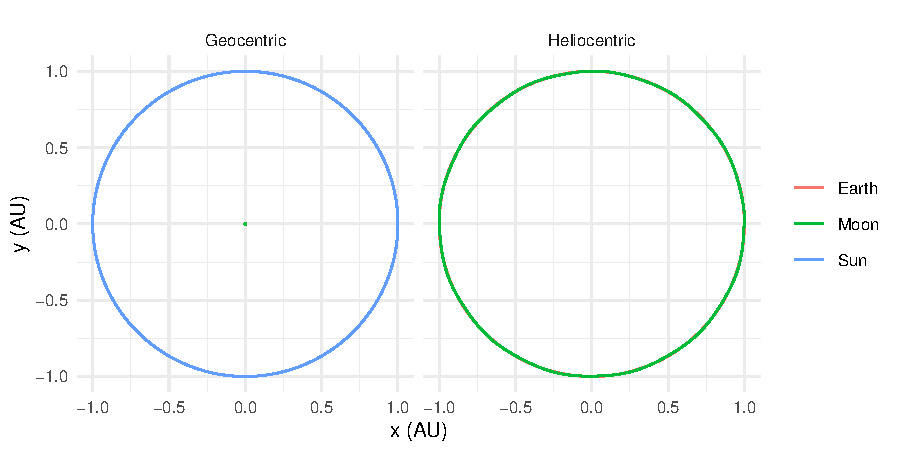
\includegraphics[width=1\linewidth,height=\textheight,keepaspectratio]{10-reference-frames_files/figure-pdf/fig-geocentric-1.pdf}

}

\caption{\label{fig-geocentric}The same year seen from the Sun (left)
and from Earth (right). In the geocentric frame the Moon's thirteen
orbits are visible and the Sun circles once.}

\end{figure}%

The shifted velocities are as useful as the positions. The Moon's speed
relative to Earth, read directly from the shifted \texttt{vx,\ vy,\ vz},
oscillates once per orbit, faster at perigee and slower at apogee, which
is Kepler's second law as a time series:

\begin{Shaded}
\begin{Highlighting}[]
\NormalTok{geo }\SpecialCharTok{|\textgreater{}}
  \FunctionTok{filter}\NormalTok{(id }\SpecialCharTok{==} \StringTok{"Moon"}\NormalTok{) }\SpecialCharTok{|\textgreater{}}
  \FunctionTok{mutate}\NormalTok{(}\AttributeTok{speed =} \FunctionTok{sqrt}\NormalTok{(vx}\SpecialCharTok{\^{}}\DecValTok{2} \SpecialCharTok{+}\NormalTok{ vy}\SpecialCharTok{\^{}}\DecValTok{2} \SpecialCharTok{+}\NormalTok{ vz}\SpecialCharTok{\^{}}\DecValTok{2}\NormalTok{)) }\SpecialCharTok{|\textgreater{}}
  \FunctionTok{ggplot}\NormalTok{(}\FunctionTok{aes}\NormalTok{(time }\SpecialCharTok{/}\NormalTok{ seconds\_per\_day, speed)) }\SpecialCharTok{+}
  \FunctionTok{geom\_line}\NormalTok{() }\SpecialCharTok{+}
  \FunctionTok{labs}\NormalTok{(}\AttributeTok{x =} \StringTok{"Day"}\NormalTok{, }\AttributeTok{y =} \StringTok{"Speed relative to Earth (m/s)"}\NormalTok{)}
\end{Highlighting}
\end{Shaded}

\begin{figure}[tbp]

\centering{

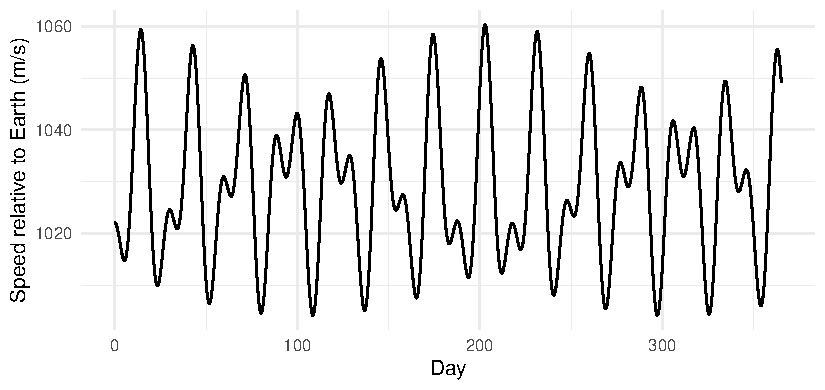
\includegraphics[width=1\linewidth,height=\textheight,keepaspectratio]{10-reference-frames_files/figure-pdf/fig-moon-speed-1.pdf}

}

\caption{\label{fig-moon-speed}The Moon's speed relative to Earth. The
monthly oscillation is the Moon's eccentricity; the slow envelope is the
Sun's perturbation.}

\end{figure}%

\section{Retrograde Mars}\label{retrograde-mars}

For most of the year Mars drifts eastward against the stars. Every 26
months it slows, stops, moves \emph{backward} for about two months,
stops again, and resumes. Ptolemy explained the loops with epicycles;
Copernicus explained them as the view from a moving platform. Here is
the Copernican explanation, run:

\begin{Shaded}
\begin{Highlighting}[]
\NormalTok{sem\_mars }\OtherTok{\textless{}{-}} \FunctionTok{create\_system}\NormalTok{() }\SpecialCharTok{|\textgreater{}}
  \FunctionTok{add\_sun}\NormalTok{() }\SpecialCharTok{|\textgreater{}}
  \FunctionTok{add\_planet}\NormalTok{(}\StringTok{"Earth"}\NormalTok{, }\AttributeTok{parent =} \StringTok{"Sun"}\NormalTok{) }\SpecialCharTok{|\textgreater{}}
  \FunctionTok{add\_planet}\NormalTok{(}\StringTok{"Mars"}\NormalTok{,  }\AttributeTok{parent =} \StringTok{"Sun"}\NormalTok{, }\AttributeTok{nu =} \DecValTok{60}\NormalTok{) }\SpecialCharTok{|\textgreater{}}
  \FunctionTok{simulate\_system}\NormalTok{(}\AttributeTok{time\_step =}\NormalTok{ seconds\_per\_day, }\AttributeTok{duration =}\NormalTok{ seconds\_per\_year }\SpecialCharTok{*} \FloatTok{2.2}\NormalTok{)}

\NormalTok{mars\_geo }\OtherTok{\textless{}{-}}\NormalTok{ sem\_mars }\SpecialCharTok{|\textgreater{}}
  \FunctionTok{shift\_reference\_frame}\NormalTok{(}\StringTok{"Earth"}\NormalTok{, }\AttributeTok{keep\_center =} \ConstantTok{FALSE}\NormalTok{) }\SpecialCharTok{|\textgreater{}}
  \FunctionTok{filter}\NormalTok{(id }\SpecialCharTok{==} \StringTok{"Mars"}\NormalTok{)}
\end{Highlighting}
\end{Shaded}

\begin{Shaded}
\begin{Highlighting}[]
\NormalTok{mars\_geo }\SpecialCharTok{|\textgreater{}}
  \FunctionTok{ggplot}\NormalTok{(}\FunctionTok{aes}\NormalTok{(x }\SpecialCharTok{/}\NormalTok{ distance\_earth\_sun, y }\SpecialCharTok{/}\NormalTok{ distance\_earth\_sun,}
             \AttributeTok{color =}\NormalTok{ time }\SpecialCharTok{/}\NormalTok{ seconds\_per\_year)) }\SpecialCharTok{+}
  \FunctionTok{geom\_path}\NormalTok{(}\AttributeTok{linewidth =} \FloatTok{0.8}\NormalTok{) }\SpecialCharTok{+}
  \FunctionTok{annotate}\NormalTok{(}\StringTok{"point"}\NormalTok{, }\AttributeTok{x =} \DecValTok{0}\NormalTok{, }\AttributeTok{y =} \DecValTok{0}\NormalTok{, }\AttributeTok{size =} \DecValTok{2}\NormalTok{) }\SpecialCharTok{+}
  \FunctionTok{coord\_equal}\NormalTok{() }\SpecialCharTok{+}
  \FunctionTok{labs}\NormalTok{(}\AttributeTok{x =} \StringTok{"x (AU)"}\NormalTok{, }\AttributeTok{y =} \StringTok{"y (AU)"}\NormalTok{, }\AttributeTok{color =} \StringTok{"Years"}\NormalTok{)}
\end{Highlighting}
\end{Shaded}

\begin{figure}[tbp]

\centering{

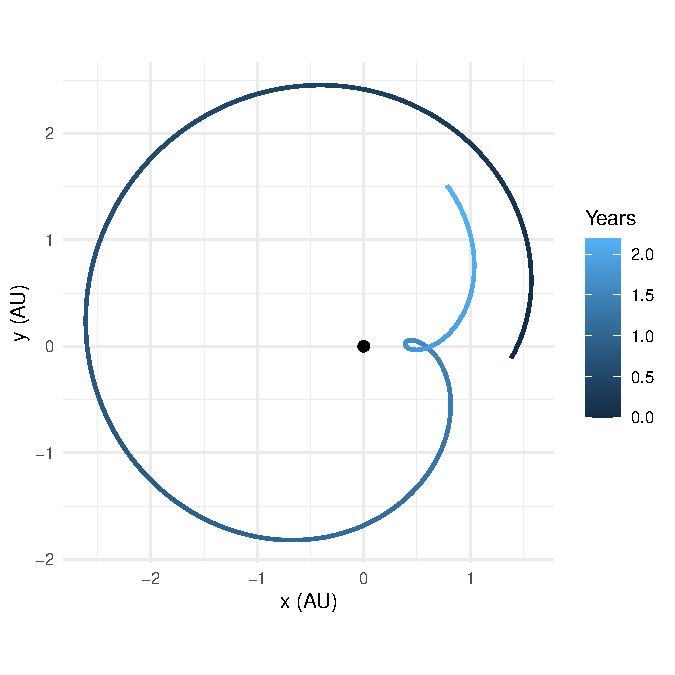
\includegraphics[width=0.65\linewidth,height=\textheight,keepaspectratio]{10-reference-frames_files/figure-pdf/fig-retrograde-1.pdf}

}

\caption{\label{fig-retrograde}Mars seen from Earth over 2.2 years. The
loop is retrograde motion: Earth, on the faster inner orbit, overtakes
Mars, and for a few weeks around opposition Mars appears to move
backward.}

\end{figure}%

The loop is real and it is nothing but geometry. We can measure it.
Mars's geocentric longitude is the angle of its position vector in
Earth's frame; it increases when Mars moves direct and decreases when it
moves retrograde:

\begin{Shaded}
\begin{Highlighting}[]
\NormalTok{retro }\OtherTok{\textless{}{-}}\NormalTok{ mars\_geo }\SpecialCharTok{|\textgreater{}}
  \FunctionTok{mutate}\NormalTok{(}\AttributeTok{longitude =} \FunctionTok{unwrap}\NormalTok{(}\FunctionTok{atan2}\NormalTok{(y, x)),}
         \AttributeTok{direction =} \FunctionTok{if\_else}\NormalTok{(}\FunctionTok{c}\NormalTok{(}\DecValTok{0}\NormalTok{, }\FunctionTok{diff}\NormalTok{(longitude)) }\SpecialCharTok{\textless{}} \DecValTok{0}\NormalTok{, }\StringTok{"retrograde"}\NormalTok{, }\StringTok{"direct"}\NormalTok{))}

\NormalTok{retro }\SpecialCharTok{|\textgreater{}}
  \FunctionTok{filter}\NormalTok{(direction }\SpecialCharTok{==} \StringTok{"retrograde"}\NormalTok{) }\SpecialCharTok{|\textgreater{}}
  \FunctionTok{summarise}\NormalTok{(}\AttributeTok{starts\_day =} \FunctionTok{min}\NormalTok{(time) }\SpecialCharTok{/}\NormalTok{ seconds\_per\_day,}
            \AttributeTok{ends\_day   =} \FunctionTok{max}\NormalTok{(time) }\SpecialCharTok{/}\NormalTok{ seconds\_per\_day,}
            \AttributeTok{duration\_days =}\NormalTok{ (}\FunctionTok{max}\NormalTok{(time) }\SpecialCharTok{{-}} \FunctionTok{min}\NormalTok{(time)) }\SpecialCharTok{/}\NormalTok{ seconds\_per\_day)}
\CommentTok{\#\textgreater{} \# A tibble: 1 x 3}
\CommentTok{\#\textgreater{}   starts\_day ends\_day duration\_days}
\CommentTok{\#\textgreater{}        \textless{}dbl\textgreater{}    \textless{}dbl\textgreater{}         \textless{}dbl\textgreater{}}
\CommentTok{\#\textgreater{} 1        598      659            61}
\end{Highlighting}
\end{Shaded}

About ten weeks of backward motion, which is what the almanacs list, and
the midpoint is the opposition, when Earth passes directly between Mars
and the Sun. The retrograde interval is \emph{always} centered on
opposition. Ptolemy's model had to build that coincidence in by hand, by
tying the epicycle's rotation to the Sun's; Copernicus's gets it for
free, because the loop \emph{is} Earth's motion.

\section{The Moon's path around the
Sun}\label{the-moons-path-around-the-sun}

Here is a puzzle that trips up almost everyone. From Earth, the Moon
goes around us in a circle. From the Sun, what does its path look like?
The tempting answer is a wavy line, looping back on itself as the Moon
swings around Earth. The actual answer is that the Moon's heliocentric
path is \emph{everywhere concave toward the Sun}: it never loops, never
even straightens out, and looks like a slightly wobbly circle. Chapter 3
gave the reason: the Sun's pull on the Moon is more than twice Earth's,
so the Moon's acceleration always points mostly at the Sun, and a path
whose acceleration always points toward a point is always curving toward
that point.

The simulation lets us check the sign of the curvature directly. A curve
bends toward the side its acceleration points to, and the direction of
bending is given by the sign of \(\mathbf{v}\times\mathbf{a}\). For a
path that always bends toward the origin,
\((\mathbf{v}\times\mathbf{a})_z\) never changes sign. Estimate
\(\mathbf{a}\) by differencing the velocity:

\begin{Shaded}
\begin{Highlighting}[]
\NormalTok{sem }\SpecialCharTok{|\textgreater{}}
  \FunctionTok{filter}\NormalTok{(id }\SpecialCharTok{==} \StringTok{"Moon"}\NormalTok{) }\SpecialCharTok{|\textgreater{}}
  \FunctionTok{mutate}\NormalTok{(}\AttributeTok{ax =} \FunctionTok{c}\NormalTok{(}\ConstantTok{NA}\NormalTok{, }\FunctionTok{diff}\NormalTok{(vx)) }\SpecialCharTok{/}\NormalTok{ seconds\_per\_hour,}
         \AttributeTok{ay =} \FunctionTok{c}\NormalTok{(}\ConstantTok{NA}\NormalTok{, }\FunctionTok{diff}\NormalTok{(vy)) }\SpecialCharTok{/}\NormalTok{ seconds\_per\_hour,}
         \AttributeTok{curvature\_sign =} \FunctionTok{sign}\NormalTok{(vx }\SpecialCharTok{*}\NormalTok{ ay }\SpecialCharTok{{-}}\NormalTok{ vy }\SpecialCharTok{*}\NormalTok{ ax)) }\SpecialCharTok{|\textgreater{}}
  \FunctionTok{count}\NormalTok{(curvature\_sign)}
\CommentTok{\#\textgreater{} \# A tibble: 2 x 2}
\CommentTok{\#\textgreater{}   curvature\_sign     n}
\CommentTok{\#\textgreater{}            \textless{}dbl\textgreater{} \textless{}int\textgreater{}}
\CommentTok{\#\textgreater{} 1              1  8766}
\CommentTok{\#\textgreater{} 2             NA     1}
\end{Highlighting}
\end{Shaded}

Every single step curves the same way. Compare Earth seen from the
Moon's frame in the next exercise: there the Sun's effect cancels (both
bodies fall toward it together) and the loop is a loop.

\section{Two sunsets}\label{two-sunsets}

Kepler-16b is a real planet with two suns. From its surface, what does
the sky do? Rebuild the system from Chapter 9 and shift to the planet:

\begin{Shaded}
\begin{Highlighting}[]
\NormalTok{AU  }\OtherTok{\textless{}{-}}\NormalTok{ distance\_earth\_sun}
\NormalTok{m\_A }\OtherTok{\textless{}{-}} \FloatTok{0.69} \SpecialCharTok{*}\NormalTok{ mass\_sun}
\NormalTok{m\_B }\OtherTok{\textless{}{-}} \FloatTok{0.20} \SpecialCharTok{*}\NormalTok{ mass\_sun}
\NormalTok{m\_p }\OtherTok{\textless{}{-}} \FloatTok{0.333} \SpecialCharTok{*}\NormalTok{ mass\_jupiter}

\NormalTok{add\_eccentric\_binary }\OtherTok{\textless{}{-}} \ControlFlowTok{function}\NormalTok{(system, m\_A, m\_B, a\_bin, e, ids) \{}
\NormalTok{  M   }\OtherTok{\textless{}{-}}\NormalTok{ m\_A }\SpecialCharTok{+}\NormalTok{ m\_B}
\NormalTok{  d\_p }\OtherTok{\textless{}{-}}\NormalTok{ a\_bin }\SpecialCharTok{*}\NormalTok{ (}\DecValTok{1} \SpecialCharTok{{-}}\NormalTok{ e)}
\NormalTok{  u\_p }\OtherTok{\textless{}{-}} \FunctionTok{sqrt}\NormalTok{(gravitational\_constant }\SpecialCharTok{*}\NormalTok{ M }\SpecialCharTok{/}\NormalTok{ a\_bin }\SpecialCharTok{*}\NormalTok{ (}\DecValTok{1} \SpecialCharTok{+}\NormalTok{ e) }\SpecialCharTok{/}\NormalTok{ (}\DecValTok{1} \SpecialCharTok{{-}}\NormalTok{ e))}
\NormalTok{  system }\SpecialCharTok{|\textgreater{}}
    \FunctionTok{add\_body}\NormalTok{(ids[}\DecValTok{1}\NormalTok{], }\AttributeTok{mass =}\NormalTok{ m\_A, }\AttributeTok{x =}\NormalTok{  d\_p }\SpecialCharTok{*}\NormalTok{ m\_B }\SpecialCharTok{/}\NormalTok{ M, }\AttributeTok{vy =}\NormalTok{  u\_p }\SpecialCharTok{*}\NormalTok{ m\_B }\SpecialCharTok{/}\NormalTok{ M) }\SpecialCharTok{|\textgreater{}}
    \FunctionTok{add\_body}\NormalTok{(ids[}\DecValTok{2}\NormalTok{], }\AttributeTok{mass =}\NormalTok{ m\_B, }\AttributeTok{x =} \SpecialCharTok{{-}}\NormalTok{d\_p }\SpecialCharTok{*}\NormalTok{ m\_A }\SpecialCharTok{/}\NormalTok{ M, }\AttributeTok{vy =} \SpecialCharTok{{-}}\NormalTok{u\_p }\SpecialCharTok{*}\NormalTok{ m\_A }\SpecialCharTok{/}\NormalTok{ M)}
\NormalTok{\}}

\NormalTok{r\_p }\OtherTok{\textless{}{-}} \FloatTok{0.7048} \SpecialCharTok{*}\NormalTok{ AU}
\NormalTok{kepler16 }\OtherTok{\textless{}{-}} \FunctionTok{create\_system}\NormalTok{() }\SpecialCharTok{|\textgreater{}}
  \FunctionTok{add\_eccentric\_binary}\NormalTok{(m\_A, m\_B, }\AttributeTok{a\_bin =} \FloatTok{0.2243} \SpecialCharTok{*}\NormalTok{ AU, }\AttributeTok{e =} \FloatTok{0.159}\NormalTok{,}
                       \AttributeTok{ids =} \FunctionTok{c}\NormalTok{(}\StringTok{"Kepler{-}16A"}\NormalTok{, }\StringTok{"Kepler{-}16B"}\NormalTok{)) }\SpecialCharTok{|\textgreater{}}
  \FunctionTok{add\_body}\NormalTok{(}\StringTok{"Kepler{-}16b"}\NormalTok{, }\AttributeTok{mass =}\NormalTok{ m\_p, }\AttributeTok{x =}\NormalTok{ r\_p,}
           \AttributeTok{vy =} \FunctionTok{sqrt}\NormalTok{(gravitational\_constant }\SpecialCharTok{*}\NormalTok{ (m\_A }\SpecialCharTok{+}\NormalTok{ m\_B) }\SpecialCharTok{/}\NormalTok{ r\_p)) }\SpecialCharTok{|\textgreater{}}
  \FunctionTok{simulate\_system}\NormalTok{(}\AttributeTok{time\_step =}\NormalTok{ seconds\_per\_hour, }\AttributeTok{duration =}\NormalTok{ seconds\_per\_year)}

\NormalTok{from\_planet }\OtherTok{\textless{}{-}}\NormalTok{ kepler16 }\SpecialCharTok{|\textgreater{}}
  \FunctionTok{shift\_reference\_frame}\NormalTok{(}\StringTok{"Kepler{-}16b"}\NormalTok{, }\AttributeTok{keep\_center =} \ConstantTok{FALSE}\NormalTok{)}
\end{Highlighting}
\end{Shaded}

\begin{Shaded}
\begin{Highlighting}[]
\NormalTok{from\_planet }\SpecialCharTok{|\textgreater{}}
  \FunctionTok{ggplot}\NormalTok{(}\FunctionTok{aes}\NormalTok{(x }\SpecialCharTok{/}\NormalTok{ AU, y }\SpecialCharTok{/}\NormalTok{ AU, }\AttributeTok{color =}\NormalTok{ id)) }\SpecialCharTok{+}
  \FunctionTok{geom\_path}\NormalTok{(}\AttributeTok{linewidth =} \FloatTok{0.6}\NormalTok{) }\SpecialCharTok{+}
  \FunctionTok{annotate}\NormalTok{(}\StringTok{"point"}\NormalTok{, }\AttributeTok{x =} \DecValTok{0}\NormalTok{, }\AttributeTok{y =} \DecValTok{0}\NormalTok{, }\AttributeTok{size =} \DecValTok{2}\NormalTok{) }\SpecialCharTok{+}
  \FunctionTok{coord\_equal}\NormalTok{() }\SpecialCharTok{+}
  \FunctionTok{labs}\NormalTok{(}\AttributeTok{x =} \StringTok{"x (AU)"}\NormalTok{, }\AttributeTok{y =} \StringTok{"y (AU)"}\NormalTok{, }\AttributeTok{color =} \ConstantTok{NULL}\NormalTok{)}
\end{Highlighting}
\end{Shaded}

\begin{figure}[tbp]

\centering{

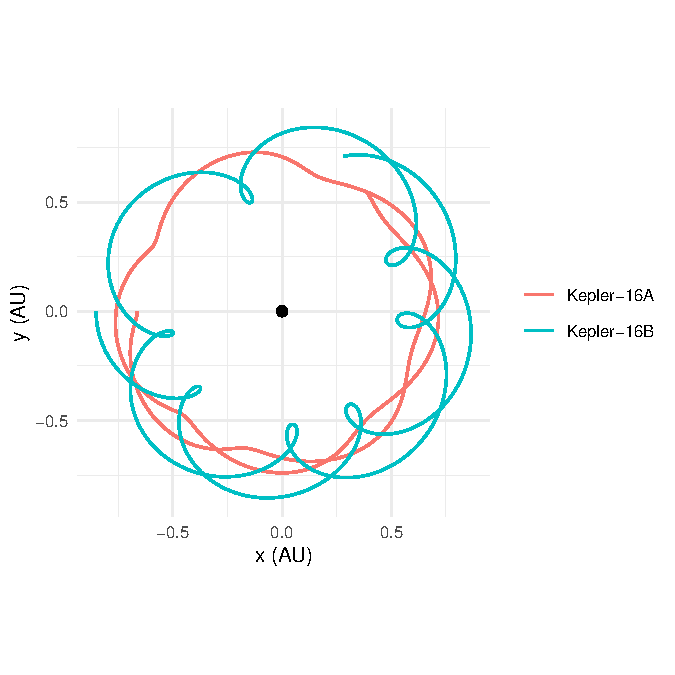
\includegraphics[width=0.65\linewidth,height=\textheight,keepaspectratio]{10-reference-frames_files/figure-pdf/fig-double-sunset-1.pdf}

}

\caption{\label{fig-double-sunset}Kepler-16's two stars as seen from the
planet over one year. Each star's path is the binary's 41-day orbit
wound around the planet's 229-day orbit.}

\end{figure}%

The spirograph pattern is two motions combined: the stars circle the
planet once per planetary year (which is the planet's own orbit, seen
from the planet), and they circle each other every 41 days on top of it.
The quantity an inhabitant would notice is the angle between the two
suns in the sky. With both stars' positions relative to the planet, that
is one arccosine:

\begin{Shaded}
\begin{Highlighting}[]
\NormalTok{star\_a }\OtherTok{\textless{}{-}}\NormalTok{ from\_planet }\SpecialCharTok{|\textgreater{}} \FunctionTok{filter}\NormalTok{(id }\SpecialCharTok{==} \StringTok{"Kepler{-}16A"}\NormalTok{) }\SpecialCharTok{|\textgreater{}} \FunctionTok{select}\NormalTok{(time, }\AttributeTok{xa =}\NormalTok{ x, }\AttributeTok{ya =}\NormalTok{ y, }\AttributeTok{za =}\NormalTok{ z)}
\NormalTok{star\_b }\OtherTok{\textless{}{-}}\NormalTok{ from\_planet }\SpecialCharTok{|\textgreater{}} \FunctionTok{filter}\NormalTok{(id }\SpecialCharTok{==} \StringTok{"Kepler{-}16B"}\NormalTok{) }\SpecialCharTok{|\textgreater{}} \FunctionTok{select}\NormalTok{(time, }\AttributeTok{xb =}\NormalTok{ x, }\AttributeTok{yb =}\NormalTok{ y, }\AttributeTok{zb =}\NormalTok{ z)}

\FunctionTok{inner\_join}\NormalTok{(star\_a, star\_b, }\AttributeTok{by =} \StringTok{"time"}\NormalTok{) }\SpecialCharTok{|\textgreater{}}
  \FunctionTok{mutate}\NormalTok{(}\AttributeTok{cos\_sep =}\NormalTok{ (xa }\SpecialCharTok{*}\NormalTok{ xb }\SpecialCharTok{+}\NormalTok{ ya }\SpecialCharTok{*}\NormalTok{ yb }\SpecialCharTok{+}\NormalTok{ za }\SpecialCharTok{*}\NormalTok{ zb) }\SpecialCharTok{/}
\NormalTok{                   (}\FunctionTok{sqrt}\NormalTok{(xa}\SpecialCharTok{\^{}}\DecValTok{2} \SpecialCharTok{+}\NormalTok{ ya}\SpecialCharTok{\^{}}\DecValTok{2} \SpecialCharTok{+}\NormalTok{ za}\SpecialCharTok{\^{}}\DecValTok{2}\NormalTok{) }\SpecialCharTok{*} \FunctionTok{sqrt}\NormalTok{(xb}\SpecialCharTok{\^{}}\DecValTok{2} \SpecialCharTok{+}\NormalTok{ yb}\SpecialCharTok{\^{}}\DecValTok{2} \SpecialCharTok{+}\NormalTok{ zb}\SpecialCharTok{\^{}}\DecValTok{2}\NormalTok{)),}
         \AttributeTok{separation\_deg =} \FunctionTok{acos}\NormalTok{(cos\_sep) }\SpecialCharTok{*} \DecValTok{180} \SpecialCharTok{/}\NormalTok{ pi) }\SpecialCharTok{|\textgreater{}}
  \FunctionTok{ggplot}\NormalTok{(}\FunctionTok{aes}\NormalTok{(time }\SpecialCharTok{/}\NormalTok{ seconds\_per\_day, separation\_deg)) }\SpecialCharTok{+}
  \FunctionTok{geom\_line}\NormalTok{() }\SpecialCharTok{+}
  \FunctionTok{labs}\NormalTok{(}\AttributeTok{x =} \StringTok{"Day"}\NormalTok{, }\AttributeTok{y =} \StringTok{"Separation of the two suns (degrees)"}\NormalTok{)}
\end{Highlighting}
\end{Shaded}

\begin{figure}[tbp]

\centering{

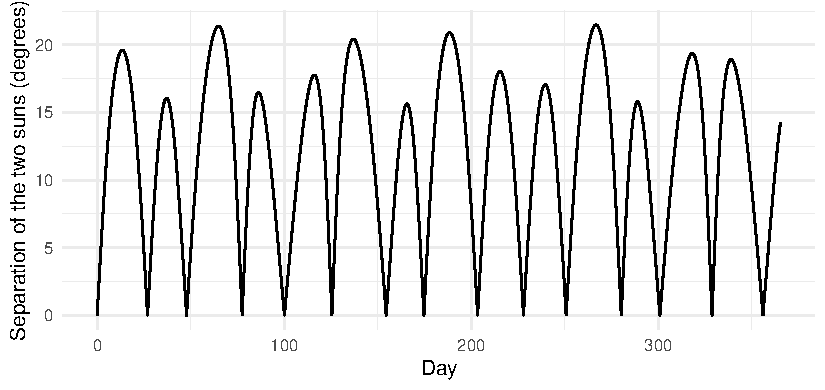
\includegraphics[width=1\linewidth,height=\textheight,keepaspectratio]{10-reference-frames_files/figure-pdf/fig-sun-separation-1.pdf}

}

\caption{\label{fig-sun-separation}Angular separation of Kepler-16's two
stars as seen from the planet. They swing apart and together every 41
days, never reaching more than about twenty degrees apart.}

\end{figure}%

Twice every 41 days the two suns line up (separation near zero, one
eclipsing the other) and twice they stand as far apart as they ever get,
about forty Moon-widths. A double sunset on Kepler-16b would be two suns
a hand's width apart going down together, with the gap between them
changing noticeably from one week to the next.

\section{A rotating frame, by hand}\label{a-rotating-frame-by-hand}

Every frame so far has been a translation: the origin moves, the axes do
not turn. There is one more kind of frame that matters in orbital
mechanics, and it is the one in which a binary star, or the Sun and
Jupiter, stand \emph{still}: a frame that rotates with them. In a
rotating frame the dynamics picks up centrifugal and Coriolis terms, and
the five famous equilibrium points of the three-body problem, the
Lagrange points, are the places where those terms balance gravity. The
package has no rotating-frame function, but dplyr does not need one. If
the frame rotates at angular rate \(\omega\) about the \(z\) axis, the
co-rotating coordinates are

\begin{equation}\protect\phantomsection\label{eq-corotating}{
x' = x\cos\omega t + y\sin\omega t, \qquad y' = -x\sin\omega t + y\cos\omega t,
}\end{equation}

which just undoes the rotation that has accumulated by time \(t\).

Set up the Sun and Jupiter as a circular binary about their barycenter
(Chapter 9's \texttt{add\_binary()}), and a small body at the \(L_4\)
point, which sits at the third corner of an equilateral triangle with
the two masses, 60 degrees ahead of Jupiter. A body exactly at \(L_4\)
moving at exactly the frame's rotation speed stays there forever; nudge
it slightly, and it wanders around \(L_4\) on a \emph{tadpole} orbit.
That is where the Trojan asteroids live.

\begin{Shaded}
\begin{Highlighting}[]
\NormalTok{add\_binary }\OtherTok{\textless{}{-}} \ControlFlowTok{function}\NormalTok{(system, m\_A, m\_B, d, ids) \{}
\NormalTok{  r\_A }\OtherTok{\textless{}{-}}\NormalTok{ d }\SpecialCharTok{*}\NormalTok{ m\_B }\SpecialCharTok{/}\NormalTok{ (m\_A }\SpecialCharTok{+}\NormalTok{ m\_B); r\_B }\OtherTok{\textless{}{-}}\NormalTok{ d }\SpecialCharTok{*}\NormalTok{ m\_A }\SpecialCharTok{/}\NormalTok{ (m\_A }\SpecialCharTok{+}\NormalTok{ m\_B)}
\NormalTok{  v\_A }\OtherTok{\textless{}{-}} \FunctionTok{sqrt}\NormalTok{(gravitational\_constant }\SpecialCharTok{*}\NormalTok{ m\_B}\SpecialCharTok{\^{}}\DecValTok{2} \SpecialCharTok{/}\NormalTok{ ((m\_A }\SpecialCharTok{+}\NormalTok{ m\_B) }\SpecialCharTok{*}\NormalTok{ d))}
\NormalTok{  v\_B }\OtherTok{\textless{}{-}} \FunctionTok{sqrt}\NormalTok{(gravitational\_constant }\SpecialCharTok{*}\NormalTok{ m\_A}\SpecialCharTok{\^{}}\DecValTok{2} \SpecialCharTok{/}\NormalTok{ ((m\_A }\SpecialCharTok{+}\NormalTok{ m\_B) }\SpecialCharTok{*}\NormalTok{ d))}
\NormalTok{  system }\SpecialCharTok{|\textgreater{}}
    \FunctionTok{add\_body}\NormalTok{(ids[}\DecValTok{1}\NormalTok{], }\AttributeTok{mass =}\NormalTok{ m\_A, }\AttributeTok{x =}\NormalTok{  r\_A, }\AttributeTok{vy =}\NormalTok{  v\_A) }\SpecialCharTok{|\textgreater{}}
    \FunctionTok{add\_body}\NormalTok{(ids[}\DecValTok{2}\NormalTok{], }\AttributeTok{mass =}\NormalTok{ m\_B, }\AttributeTok{x =} \SpecialCharTok{{-}}\NormalTok{r\_B, }\AttributeTok{vy =} \SpecialCharTok{{-}}\NormalTok{v\_B)}
\NormalTok{\}}

\NormalTok{d     }\OtherTok{\textless{}{-}}\NormalTok{ distance\_jupiter\_sun}
\NormalTok{omega }\OtherTok{\textless{}{-}} \FunctionTok{sqrt}\NormalTok{(gravitational\_constant }\SpecialCharTok{*}\NormalTok{ (mass\_sun }\SpecialCharTok{+}\NormalTok{ mass\_jupiter) }\SpecialCharTok{/}\NormalTok{ d}\SpecialCharTok{\^{}}\DecValTok{3}\NormalTok{)}

\CommentTok{\# Jupiter sits at angle 180 degrees moving counterclockwise; L4 is 60 degrees}
\CommentTok{\# ahead of it, at the apex of the equilateral triangle below the x axis.}
\NormalTok{sun\_x }\OtherTok{\textless{}{-}}\NormalTok{ d }\SpecialCharTok{*}\NormalTok{ mass\_jupiter }\SpecialCharTok{/}\NormalTok{ (mass\_sun }\SpecialCharTok{+}\NormalTok{ mass\_jupiter)}
\NormalTok{jup\_x }\OtherTok{\textless{}{-}} \SpecialCharTok{{-}}\NormalTok{d }\SpecialCharTok{*}\NormalTok{ mass\_sun }\SpecialCharTok{/}\NormalTok{ (mass\_sun }\SpecialCharTok{+}\NormalTok{ mass\_jupiter)}
\NormalTok{L4    }\OtherTok{\textless{}{-}} \FunctionTok{c}\NormalTok{((sun\_x }\SpecialCharTok{+}\NormalTok{ jup\_x) }\SpecialCharTok{/} \DecValTok{2}\NormalTok{, }\SpecialCharTok{{-}}\FunctionTok{sqrt}\NormalTok{(}\DecValTok{3}\NormalTok{) }\SpecialCharTok{/} \DecValTok{2} \SpecialCharTok{*}\NormalTok{ d)}
\NormalTok{p     }\OtherTok{\textless{}{-}}\NormalTok{ L4 }\SpecialCharTok{*} \FloatTok{1.02}                            \CommentTok{\# nudged 2\% outward}
\NormalTok{v     }\OtherTok{\textless{}{-}}\NormalTok{ omega }\SpecialCharTok{*} \FunctionTok{c}\NormalTok{(}\SpecialCharTok{{-}}\NormalTok{p[}\DecValTok{2}\NormalTok{], p[}\DecValTok{1}\NormalTok{])               }\CommentTok{\# rigid co{-}rotation}

\NormalTok{trojan }\OtherTok{\textless{}{-}} \FunctionTok{create\_system}\NormalTok{() }\SpecialCharTok{|\textgreater{}}
  \FunctionTok{add\_binary}\NormalTok{(mass\_sun, mass\_jupiter, d, }\AttributeTok{ids =} \FunctionTok{c}\NormalTok{(}\StringTok{"Sun"}\NormalTok{, }\StringTok{"Jupiter"}\NormalTok{)) }\SpecialCharTok{|\textgreater{}}
  \FunctionTok{add\_body}\NormalTok{(}\StringTok{"Trojan"}\NormalTok{, }\AttributeTok{mass =} \FloatTok{1e15}\NormalTok{, }\AttributeTok{x =}\NormalTok{ p[}\DecValTok{1}\NormalTok{], }\AttributeTok{y =}\NormalTok{ p[}\DecValTok{2}\NormalTok{], }\AttributeTok{vx =}\NormalTok{ v[}\DecValTok{1}\NormalTok{], }\AttributeTok{vy =}\NormalTok{ v[}\DecValTok{2}\NormalTok{]) }\SpecialCharTok{|\textgreater{}}
  \FunctionTok{simulate\_system}\NormalTok{(}\AttributeTok{time\_step =}\NormalTok{ seconds\_per\_day, }\AttributeTok{duration =}\NormalTok{ seconds\_per\_year }\SpecialCharTok{*} \DecValTok{150}\NormalTok{)}
\end{Highlighting}
\end{Shaded}

\begin{Shaded}
\begin{Highlighting}[]
\NormalTok{trojan }\SpecialCharTok{|\textgreater{}}
  \FunctionTok{mutate}\NormalTok{(}\AttributeTok{theta =}\NormalTok{ omega }\SpecialCharTok{*}\NormalTok{ time,}
         \AttributeTok{xr =}\NormalTok{  x }\SpecialCharTok{*} \FunctionTok{cos}\NormalTok{(theta) }\SpecialCharTok{+}\NormalTok{ y }\SpecialCharTok{*} \FunctionTok{sin}\NormalTok{(theta),}
         \AttributeTok{yr =} \SpecialCharTok{{-}}\NormalTok{x }\SpecialCharTok{*} \FunctionTok{sin}\NormalTok{(theta) }\SpecialCharTok{+}\NormalTok{ y }\SpecialCharTok{*} \FunctionTok{cos}\NormalTok{(theta)) }\SpecialCharTok{|\textgreater{}}
  \FunctionTok{ggplot}\NormalTok{(}\FunctionTok{aes}\NormalTok{(xr }\SpecialCharTok{/}\NormalTok{ AU, yr }\SpecialCharTok{/}\NormalTok{ AU, }\AttributeTok{color =}\NormalTok{ id)) }\SpecialCharTok{+}
  \FunctionTok{geom\_path}\NormalTok{() }\SpecialCharTok{+}
  \FunctionTok{annotate}\NormalTok{(}\StringTok{"point"}\NormalTok{, }\AttributeTok{x =}\NormalTok{ L4[}\DecValTok{1}\NormalTok{] }\SpecialCharTok{/}\NormalTok{ AU, }\AttributeTok{y =}\NormalTok{ L4[}\DecValTok{2}\NormalTok{] }\SpecialCharTok{/}\NormalTok{ AU, }\AttributeTok{shape =} \DecValTok{4}\NormalTok{, }\AttributeTok{size =} \DecValTok{3}\NormalTok{) }\SpecialCharTok{+}
  \FunctionTok{coord\_equal}\NormalTok{() }\SpecialCharTok{+}
  \FunctionTok{labs}\NormalTok{(}\AttributeTok{x =} \StringTok{"x (AU, rotating)"}\NormalTok{, }\AttributeTok{y =} \StringTok{"y (AU, rotating)"}\NormalTok{, }\AttributeTok{color =} \ConstantTok{NULL}\NormalTok{)}
\end{Highlighting}
\end{Shaded}

\begin{figure}[tbp]

\centering{

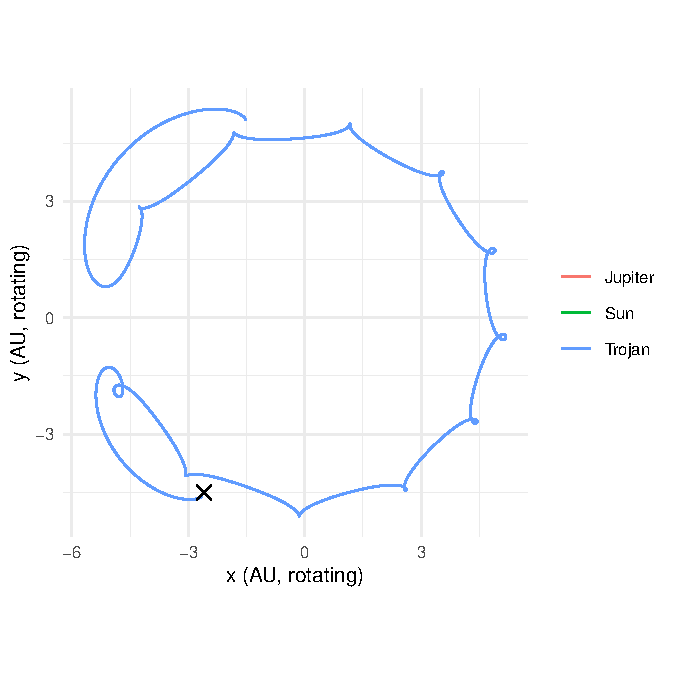
\includegraphics[width=0.65\linewidth,height=\textheight,keepaspectratio]{10-reference-frames_files/figure-pdf/fig-trojan-1.pdf}

}

\caption{\label{fig-trojan}The Sun-Jupiter system in the frame rotating
with Jupiter, over 150 years. The Sun and Jupiter are fixed points; the
nudged Trojan librates around \(L_4\) on a tadpole orbit.}

\end{figure}%

In the inertial frame the Trojan's path is an unremarkable near-circle
at Jupiter's distance. In the rotating frame it is a closed loop around
a point in empty space, held there by nothing but the combined gravity
of the Sun and Jupiter in a frame where that gravity has to fight the
centrifugal force. The \(\times\) marks \(L_4\). Jupiter has about ten
thousand known Trojans doing exactly this, and Earth has two. Chapter 11
looks at the other Lagrange points, which are not so hospitable.

\begin{tcolorbox}[enhanced jigsaw, arc=.35mm, bottomrule=.15mm, bottomtitle=1mm, breakable, colback=white, colbacktitle=quarto-callout-tip-color!10!white, colframe=quarto-callout-tip-color-frame, coltitle=black, left=2mm, leftrule=.75mm, opacityback=0, opacitybacktitle=0.6, rightrule=.15mm, title={Key results}, titlerule=0mm, toprule=.15mm, toptitle=1mm]

\begin{itemize}
\tightlist
\item
  \texttt{shift\_reference\_frame()} is a Galilean translation applied
  to the output: same physics, different observer. The frame it produces
  is accelerated, which is fine for looking and not for computing
  forces.
\item
  Retrograde motion is the view of an outer planet from a faster inner
  one; the retrograde interval is centered on opposition.
\item
  The Moon's heliocentric path is always concave toward the Sun, because
  the Sun's pull on it exceeds Earth's.
\item
  Rotating frame: \(x' = x\cos\omega t + y\sin\omega t\),
  \(y' = -x\sin\omega t + y\cos\omega t\). In the frame co-rotating with
  a circular binary, the Lagrange points are fixed and \(L_4\), \(L_5\)
  are stable.
\end{itemize}

\end{tcolorbox}

\chapter{Chaos and the Three-Body Problem}\label{sec-chaos}

Chapter 4 solved the two-body problem completely, on paper. Add one more
body and the paper runs out: there is no formula, and for most starting
configurations there is not even a stable outcome, only a brief dance
and then an ejection. The package documentation shows one such triple
and says that it is chaotic. This chapter measures the chaos: how fast
two nearly identical triples diverge, what a slingshot ejection does to
the energy budget, and why some three-body systems (ours, for instance)
are perfectly well behaved. It ends with the five points where a third
body can sit still, and why three of them are traps.

\section{What Poincaré proved}\label{what-poincaruxe9-proved}

\begin{tcolorbox}[enhanced jigsaw, arc=.35mm, bottomrule=.15mm, bottomtitle=1mm, breakable, colback=white, colbacktitle=quarto-callout-note-color!10!white, colframe=quarto-callout-note-color-frame, coltitle=black, left=2mm, leftrule=.75mm, opacityback=0, opacitybacktitle=0.6, rightrule=.15mm, title={Where it comes from}, titlerule=0mm, toprule=.15mm, toptitle=1mm]

In 1885 King Oscar II of Sweden offered a prize for a proof that the
solar system is stable. Henri Poincaré did not prove it. He showed
instead that the three-body problem, even in a restricted form, has
orbits so tangled that no formula of the usual kind could ever describe
them, and in the course of correcting an error in his own prize essay he
found the first example of what is now called a homoclinic tangle:
trajectories that wind around each other infinitely often, so that where
a body ends up depends on where it started with a sensitivity no
measurement can satisfy (Poincaré 1890). He later wrote of the resulting
figure that he would not even attempt to draw it. The phenomenon was
named \emph{chaos} seventy years later, when computers made it possible
to draw.

``No general solution'' does not mean the motion cannot be computed. It
means the computation cannot be shortcut. Kepler's ellipse lets you find
a planet's position a million years from now in one step; for three
bodies, the only way to find out what happens is to follow them step by
step, and the simulation is the solution.

\end{tcolorbox}

\section{Sensitive dependence,
measured}\label{sensitive-dependence-measured}

Here is the documentation's triple: three Sun-mass stars at the corners
of a triangle, with velocities that are nearly but not quite symmetric.

\begin{Shaded}
\begin{Highlighting}[]
\NormalTok{triple }\OtherTok{\textless{}{-}} \ControlFlowTok{function}\NormalTok{(}\AttributeTok{dx =} \DecValTok{0}\NormalTok{) \{}
  \FunctionTok{create\_system}\NormalTok{() }\SpecialCharTok{|\textgreater{}}
    \FunctionTok{add\_body}\NormalTok{(}\StringTok{"Star A"}\NormalTok{, }\AttributeTok{mass =} \FloatTok{1e30}\NormalTok{, }\AttributeTok{x =} \FloatTok{1e11} \SpecialCharTok{+}\NormalTok{ dx, }\AttributeTok{y =} \DecValTok{0}\NormalTok{,}
             \AttributeTok{vx =} \DecValTok{0}\NormalTok{, }\AttributeTok{vy =} \DecValTok{15000}\NormalTok{) }\SpecialCharTok{|\textgreater{}}
    \FunctionTok{add\_body}\NormalTok{(}\StringTok{"Star B"}\NormalTok{, }\AttributeTok{mass =} \FloatTok{1e30}\NormalTok{, }\AttributeTok{x =} \SpecialCharTok{{-}}\FloatTok{5e10}\NormalTok{, }\AttributeTok{y =} \FloatTok{8.66e10}\NormalTok{,}
             \AttributeTok{vx =} \SpecialCharTok{{-}}\DecValTok{12990}\NormalTok{, }\AttributeTok{vy =} \SpecialCharTok{{-}}\DecValTok{7500}\NormalTok{) }\SpecialCharTok{|\textgreater{}}
    \FunctionTok{add\_body}\NormalTok{(}\StringTok{"Star C"}\NormalTok{, }\AttributeTok{mass =} \FloatTok{1e30}\NormalTok{, }\AttributeTok{x =} \SpecialCharTok{{-}}\FloatTok{5e10}\NormalTok{, }\AttributeTok{y =} \SpecialCharTok{{-}}\FloatTok{8.66e10}\NormalTok{,}
             \AttributeTok{vx =} \DecValTok{14000}\NormalTok{, }\AttributeTok{vy =} \SpecialCharTok{{-}}\DecValTok{8000}\NormalTok{) }\SpecialCharTok{|\textgreater{}}
    \FunctionTok{simulate\_system}\NormalTok{(}\AttributeTok{time\_step =}\NormalTok{ seconds\_per\_hour, }\AttributeTok{duration =}\NormalTok{ seconds\_per\_year }\SpecialCharTok{*} \DecValTok{3}\NormalTok{)}
\NormalTok{\}}

\NormalTok{run\_1 }\OtherTok{\textless{}{-}} \FunctionTok{triple}\NormalTok{()}
\NormalTok{run\_2 }\OtherTok{\textless{}{-}} \FunctionTok{triple}\NormalTok{(}\AttributeTok{dx =} \DecValTok{1}\NormalTok{)      }\CommentTok{\# Star A starts one meter to the right}
\end{Highlighting}
\end{Shaded}

One meter, in a system a hundred billion meters across: a part in
\(10^{11}\), far below any conceivable measurement of a real star's
position. Track how far apart the two runs drift:

\begin{Shaded}
\begin{Highlighting}[]
\NormalTok{divergence }\OtherTok{\textless{}{-}} \FunctionTok{inner\_join}\NormalTok{(}
\NormalTok{  run\_1 }\SpecialCharTok{|\textgreater{}} \FunctionTok{select}\NormalTok{(time, id, x, y, z),}
\NormalTok{  run\_2 }\SpecialCharTok{|\textgreater{}} \FunctionTok{select}\NormalTok{(time, id, }\AttributeTok{x2 =}\NormalTok{ x, }\AttributeTok{y2 =}\NormalTok{ y, }\AttributeTok{z2 =}\NormalTok{ z),}
  \AttributeTok{by =} \FunctionTok{c}\NormalTok{(}\StringTok{"time"}\NormalTok{, }\StringTok{"id"}\NormalTok{)) }\SpecialCharTok{|\textgreater{}}
  \FunctionTok{mutate}\NormalTok{(}\AttributeTok{d =} \FunctionTok{sqrt}\NormalTok{((x }\SpecialCharTok{{-}}\NormalTok{ x2)}\SpecialCharTok{\^{}}\DecValTok{2} \SpecialCharTok{+}\NormalTok{ (y }\SpecialCharTok{{-}}\NormalTok{ y2)}\SpecialCharTok{\^{}}\DecValTok{2} \SpecialCharTok{+}\NormalTok{ (z }\SpecialCharTok{{-}}\NormalTok{ z2)}\SpecialCharTok{\^{}}\DecValTok{2}\NormalTok{)) }\SpecialCharTok{|\textgreater{}}
  \FunctionTok{group\_by}\NormalTok{(time) }\SpecialCharTok{|\textgreater{}}
  \FunctionTok{summarise}\NormalTok{(}\AttributeTok{separation =} \FunctionTok{sqrt}\NormalTok{(}\FunctionTok{sum}\NormalTok{(d}\SpecialCharTok{\^{}}\DecValTok{2}\NormalTok{)))}
\end{Highlighting}
\end{Shaded}

\begin{Shaded}
\begin{Highlighting}[]
\NormalTok{divergence }\SpecialCharTok{|\textgreater{}}
  \FunctionTok{ggplot}\NormalTok{(}\FunctionTok{aes}\NormalTok{(time }\SpecialCharTok{/}\NormalTok{ seconds\_per\_year, separation)) }\SpecialCharTok{+}
  \FunctionTok{geom\_line}\NormalTok{() }\SpecialCharTok{+}
  \FunctionTok{scale\_y\_log10}\NormalTok{() }\SpecialCharTok{+}
  \FunctionTok{labs}\NormalTok{(}\AttributeTok{x =} \StringTok{"Years"}\NormalTok{, }\AttributeTok{y =} \StringTok{"Separation between runs (m)"}\NormalTok{)}
\end{Highlighting}
\end{Shaded}

\begin{figure}[tbp]

\centering{

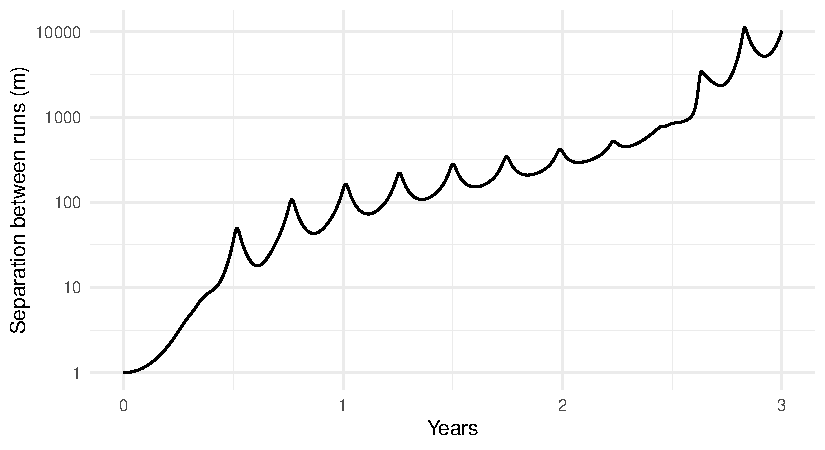
\includegraphics[width=1\linewidth,height=\textheight,keepaspectratio]{11-chaos-and-the-three-body-problem_files/figure-pdf/fig-divergence-1.pdf}

}

\caption{\label{fig-divergence}Distance in configuration space between
two runs of the same triple whose only difference is one meter in one
star's starting position. The vertical axis is logarithmic: the
straight-line section is exponential growth.}

\end{figure}%

The separation grows \emph{exponentially}: a straight line on a log
axis. That is the signature of chaos, and the slope of the line is its
rate. If the separation grows as \(\delta(t) = \delta_0 e^{t/\tau}\),
then \(\tau\) is the \emph{Lyapunov time}, the time for a small error to
grow by a factor of \(e\). Fit it on the part of the curve that is still
growing, before the separation saturates at the size of the system:

\begin{Shaded}
\begin{Highlighting}[]
\NormalTok{growth }\OtherTok{\textless{}{-}}\NormalTok{ divergence }\SpecialCharTok{|\textgreater{}}
  \FunctionTok{filter}\NormalTok{(separation }\SpecialCharTok{\textgreater{}} \FloatTok{1e3}\NormalTok{, separation }\SpecialCharTok{\textless{}} \FloatTok{1e9}\NormalTok{)}

\NormalTok{tau }\OtherTok{\textless{}{-}} \DecValTok{1} \SpecialCharTok{/} \FunctionTok{coef}\NormalTok{(}\FunctionTok{lm}\NormalTok{(}\FunctionTok{log}\NormalTok{(separation) }\SpecialCharTok{\textasciitilde{}}\NormalTok{ time, }\AttributeTok{data =}\NormalTok{ growth))[[}\StringTok{"time"}\NormalTok{]]}
\NormalTok{tau }\SpecialCharTok{/}\NormalTok{ seconds\_per\_day}
\CommentTok{\#\textgreater{} [1] 92.63501}
\end{Highlighting}
\end{Shaded}

A Lyapunov time of a few weeks. Every few weeks the uncertainty in the
system's state grows by a factor of nearly three; in a year it has grown
by a factor of \(e^{365/\tau}\), which is enormous. After the point
where the two curves saturate, the runs have nothing to do with each
other: they are two different triples that happen to share a history.

This has a practical consequence that is easy to miss. Beyond the
Lyapunov horizon, \emph{the simulation is not predicting this system}.
The integrator's own rounding errors, at the \(10^{-16}\) level, are
amplified just like the one-meter nudge, so two runs on different
computers, or the same run with a different time step, will disagree in
detail after a year or two. What the simulation does predict is the
\emph{kind} of thing that happens: the statistics of the dance, the fact
of the ejection, roughly when. For chaotic systems, those are the only
questions with answers.

\section{Slingshot}\label{slingshot}

\begin{Shaded}
\begin{Highlighting}[]
\FunctionTok{plot\_orbits}\NormalTok{(run\_1)}
\end{Highlighting}
\end{Shaded}

\begin{figure}[tbp]

\centering{

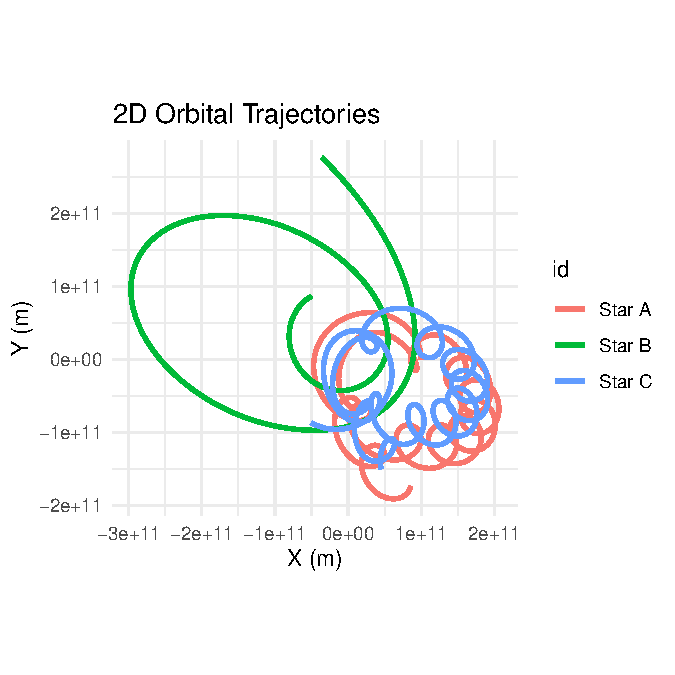
\includegraphics[width=0.65\linewidth,height=\textheight,keepaspectratio]{11-chaos-and-the-three-body-problem_files/figure-pdf/fig-triple-1.pdf}

}

\caption{\label{fig-triple}Three years of the chaotic triple. The static
picture is hard to read; the energy table below says what happened.}

\end{figure}%

The documentation says one star gets flung out. Let's make ``flung out''
precise. A body has escaped a system when its energy relative to the
rest, kinetic energy in the center-of-mass frame plus its potential
energy with every other body, is positive: it has enough speed to climb
out of the potential well of the others and keep going. Here is that
bookkeeping at a single instant:

\begin{Shaded}
\begin{Highlighting}[]
\NormalTok{body\_energies }\OtherTok{\textless{}{-}} \ControlFlowTok{function}\NormalTok{(snapshot, }\AttributeTok{G =}\NormalTok{ gravitational\_constant) \{}
\NormalTok{  M    }\OtherTok{\textless{}{-}} \FunctionTok{sum}\NormalTok{(snapshot}\SpecialCharTok{$}\NormalTok{mass)}
\NormalTok{  v\_cm }\OtherTok{\textless{}{-}} \FunctionTok{c}\NormalTok{(}\FunctionTok{sum}\NormalTok{(snapshot}\SpecialCharTok{$}\NormalTok{mass }\SpecialCharTok{*}\NormalTok{ snapshot}\SpecialCharTok{$}\NormalTok{vx),}
            \FunctionTok{sum}\NormalTok{(snapshot}\SpecialCharTok{$}\NormalTok{mass }\SpecialCharTok{*}\NormalTok{ snapshot}\SpecialCharTok{$}\NormalTok{vy),}
            \FunctionTok{sum}\NormalTok{(snapshot}\SpecialCharTok{$}\NormalTok{mass }\SpecialCharTok{*}\NormalTok{ snapshot}\SpecialCharTok{$}\NormalTok{vz)) }\SpecialCharTok{/}\NormalTok{ M}
\NormalTok{  n }\OtherTok{\textless{}{-}} \FunctionTok{nrow}\NormalTok{(snapshot)}
\NormalTok{  E }\OtherTok{\textless{}{-}} \FunctionTok{numeric}\NormalTok{(n)}
  \ControlFlowTok{for}\NormalTok{ (i }\ControlFlowTok{in} \FunctionTok{seq\_len}\NormalTok{(n)) \{}
\NormalTok{    v\_rel }\OtherTok{\textless{}{-}} \FunctionTok{c}\NormalTok{(snapshot}\SpecialCharTok{$}\NormalTok{vx[i], snapshot}\SpecialCharTok{$}\NormalTok{vy[i], snapshot}\SpecialCharTok{$}\NormalTok{vz[i]) }\SpecialCharTok{{-}}\NormalTok{ v\_cm}
\NormalTok{    KE }\OtherTok{\textless{}{-}} \FloatTok{0.5} \SpecialCharTok{*}\NormalTok{ snapshot}\SpecialCharTok{$}\NormalTok{mass[i] }\SpecialCharTok{*} \FunctionTok{sum}\NormalTok{(v\_rel}\SpecialCharTok{\^{}}\DecValTok{2}\NormalTok{)}
\NormalTok{    PE }\OtherTok{\textless{}{-}} \DecValTok{0}
    \ControlFlowTok{for}\NormalTok{ (j }\ControlFlowTok{in} \FunctionTok{seq\_len}\NormalTok{(n)[}\SpecialCharTok{{-}}\NormalTok{i]) \{}
\NormalTok{      r\_ij }\OtherTok{\textless{}{-}} \FunctionTok{sqrt}\NormalTok{((snapshot}\SpecialCharTok{$}\NormalTok{x[i] }\SpecialCharTok{{-}}\NormalTok{ snapshot}\SpecialCharTok{$}\NormalTok{x[j])}\SpecialCharTok{\^{}}\DecValTok{2} \SpecialCharTok{+}
\NormalTok{                   (snapshot}\SpecialCharTok{$}\NormalTok{y[i] }\SpecialCharTok{{-}}\NormalTok{ snapshot}\SpecialCharTok{$}\NormalTok{y[j])}\SpecialCharTok{\^{}}\DecValTok{2} \SpecialCharTok{+}
\NormalTok{                   (snapshot}\SpecialCharTok{$}\NormalTok{z[i] }\SpecialCharTok{{-}}\NormalTok{ snapshot}\SpecialCharTok{$}\NormalTok{z[j])}\SpecialCharTok{\^{}}\DecValTok{2}\NormalTok{)}
\NormalTok{      PE }\OtherTok{\textless{}{-}}\NormalTok{ PE }\SpecialCharTok{{-}}\NormalTok{ G }\SpecialCharTok{*}\NormalTok{ snapshot}\SpecialCharTok{$}\NormalTok{mass[i] }\SpecialCharTok{*}\NormalTok{ snapshot}\SpecialCharTok{$}\NormalTok{mass[j] }\SpecialCharTok{/}\NormalTok{ r\_ij}
\NormalTok{    \}}
\NormalTok{    E[i] }\OtherTok{\textless{}{-}}\NormalTok{ KE }\SpecialCharTok{+}\NormalTok{ PE}
\NormalTok{  \}}
  \FunctionTok{tibble}\NormalTok{(}\AttributeTok{id =}\NormalTok{ snapshot}\SpecialCharTok{$}\NormalTok{id, }\AttributeTok{energy =}\NormalTok{ E,}
         \AttributeTok{r\_from\_cm =} \FunctionTok{sqrt}\NormalTok{((snapshot}\SpecialCharTok{$}\NormalTok{x }\SpecialCharTok{{-}} \FunctionTok{sum}\NormalTok{(snapshot}\SpecialCharTok{$}\NormalTok{mass }\SpecialCharTok{*}\NormalTok{ snapshot}\SpecialCharTok{$}\NormalTok{x) }\SpecialCharTok{/}\NormalTok{ M)}\SpecialCharTok{\^{}}\DecValTok{2} \SpecialCharTok{+}
\NormalTok{                          (snapshot}\SpecialCharTok{$}\NormalTok{y }\SpecialCharTok{{-}} \FunctionTok{sum}\NormalTok{(snapshot}\SpecialCharTok{$}\NormalTok{mass }\SpecialCharTok{*}\NormalTok{ snapshot}\SpecialCharTok{$}\NormalTok{y) }\SpecialCharTok{/}\NormalTok{ M)}\SpecialCharTok{\^{}}\DecValTok{2}\NormalTok{))}
\NormalTok{\}}

\FunctionTok{bind\_rows}\NormalTok{(}
\NormalTok{  run\_1 }\SpecialCharTok{|\textgreater{}} \FunctionTok{filter}\NormalTok{(time }\SpecialCharTok{==} \FunctionTok{min}\NormalTok{(time)) }\SpecialCharTok{|\textgreater{}} \FunctionTok{body\_energies}\NormalTok{() }\SpecialCharTok{|\textgreater{}} \FunctionTok{mutate}\NormalTok{(}\AttributeTok{when =} \StringTok{"start"}\NormalTok{),}
\NormalTok{  run\_1 }\SpecialCharTok{|\textgreater{}} \FunctionTok{filter}\NormalTok{(time }\SpecialCharTok{==} \FunctionTok{max}\NormalTok{(time)) }\SpecialCharTok{|\textgreater{}} \FunctionTok{body\_energies}\NormalTok{() }\SpecialCharTok{|\textgreater{}} \FunctionTok{mutate}\NormalTok{(}\AttributeTok{when =} \StringTok{"end"}\NormalTok{)}
\NormalTok{) }\SpecialCharTok{|\textgreater{}}
  \FunctionTok{arrange}\NormalTok{(id, when)}
\CommentTok{\#\textgreater{} \# A tibble: 6 x 4}
\CommentTok{\#\textgreater{}   id       energy     r\_from\_cm when }
\CommentTok{\#\textgreater{}   \textless{}chr\textgreater{}     \textless{}dbl\textgreater{}         \textless{}dbl\textgreater{} \textless{}chr\textgreater{}}
\CommentTok{\#\textgreater{} 1 Star A {-}1.31e39 166443322355. end  }
\CommentTok{\#\textgreater{} 2 Star A {-}6.56e38 100000000000  start}
\CommentTok{\#\textgreater{} 3 Star B {-}1.93e38 299192659248. end  }
\CommentTok{\#\textgreater{} 4 Star B {-}6.55e38  99997799976. start}
\CommentTok{\#\textgreater{} 5 Star C {-}1.03e39 134679821974. end  }
\CommentTok{\#\textgreater{} 6 Star C {-}6.47e38  99997799976. start}
\end{Highlighting}
\end{Shaded}

At the start all three stars are bound to the system. At the end, a star
whose energy is positive is leaving and never coming back, and it is the
one farthest from the center of mass. Where did its energy come from?
Total energy is conserved (check it with
\texttt{conserved\_quantities()}), so if one star gained enough to
escape, the other two lost the same amount: the pair left behind is on a
tighter, more negative-energy orbit than any pair was at the start. This
is the \emph{slingshot}, and it is the basic mechanism of stellar
dynamics. In a star cluster, three-body encounters harden binaries and
eject single stars, and over millions of years that is how clusters lose
members and how their cores contract. We can look at the binary that
remains:

\begin{Shaded}
\begin{Highlighting}[]
\NormalTok{final }\OtherTok{\textless{}{-}}\NormalTok{ run\_1 }\SpecialCharTok{|\textgreater{}} \FunctionTok{filter}\NormalTok{(time }\SpecialCharTok{==} \FunctionTok{max}\NormalTok{(time)) }\SpecialCharTok{|\textgreater{}} \FunctionTok{body\_energies}\NormalTok{()}
\NormalTok{bound }\OtherTok{\textless{}{-}}\NormalTok{ final }\SpecialCharTok{|\textgreater{}} \FunctionTok{filter}\NormalTok{(energy }\SpecialCharTok{\textless{}} \DecValTok{0}\NormalTok{) }\SpecialCharTok{|\textgreater{}} \FunctionTok{pull}\NormalTok{(id)}
\NormalTok{bound}
\CommentTok{\#\textgreater{} [1] "Star A" "Star B" "Star C"}
\end{Highlighting}
\end{Shaded}

\begin{Shaded}
\begin{Highlighting}[]
\ControlFlowTok{if}\NormalTok{ (}\FunctionTok{length}\NormalTok{(bound) }\SpecialCharTok{==} \DecValTok{2}\NormalTok{) \{}
\NormalTok{  last\_year }\OtherTok{\textless{}{-}}\NormalTok{ run\_1 }\SpecialCharTok{|\textgreater{}} \FunctionTok{filter}\NormalTok{(time }\SpecialCharTok{\textgreater{}} \FunctionTok{max}\NormalTok{(time) }\SpecialCharTok{{-}}\NormalTok{ seconds\_per\_year)}
  \FunctionTok{get\_orbital\_elements}\NormalTok{(last\_year, bound[}\DecValTok{2}\NormalTok{], bound[}\DecValTok{1}\NormalTok{],}
                       \AttributeTok{mu =}\NormalTok{ gravitational\_constant }\SpecialCharTok{*} \FloatTok{2e30}\NormalTok{) }\SpecialCharTok{|\textgreater{}}
    \FunctionTok{filter}\NormalTok{(time }\SpecialCharTok{==} \FunctionTok{max}\NormalTok{(time)) }\SpecialCharTok{|\textgreater{}}
    \FunctionTok{mutate}\NormalTok{(}\AttributeTok{a\_AU =}\NormalTok{ a }\SpecialCharTok{/}\NormalTok{ distance\_earth\_sun) }\SpecialCharTok{|\textgreater{}}
    \FunctionTok{select}\NormalTok{(a\_AU, e)}
\NormalTok{\}}
\end{Highlighting}
\end{Shaded}

The survivors' orbit is a two-body ellipse, and from here on, unless the
third star comes back, Chapter 4 describes them exactly. A typical
outcome of a three-body breakup is a binary with a substantial
eccentricity: the third body did not leave politely.

\section{Why the Sun, Earth, and Moon are not
chaotic}\label{why-the-sun-earth-and-moon-are-not-chaotic}

If three bodies are chaotic, how does the Moon manage? The
Sun-Earth-Moon system is a three-body system, and the Moon has been in
orbit for four billion years. The answer is \emph{hierarchy}: the Moon
is close to Earth and both are far from the Sun, so the Moon's orbit is
a two-body orbit about Earth with a small perturbation, and Earth's is a
two-body orbit about the Sun with a small perturbation. Chaos needs the
three bodies to interact as equals.

How close is close enough? Think about it in the frame rotating with
Earth around the Sun. A satellite of Earth is held by Earth's gravity,
\(G m_\oplus / r^2\), and pulled away by the difference between the
Sun's gravity at its position and at Earth's, plus the centrifugal
effect of the rotation. Along the Sun-Earth line, that \emph{tidal}
acceleration works out to \(3\,G M_\odot\, r / R^3\), where \(R\) is
Earth's distance from the Sun (two parts from the Sun's gradient, one
from the centrifugal term). The two balance at

\begin{equation}\protect\phantomsection\label{eq-hill}{
r_{\mathrm{H}} = R\left(\frac{m_\oplus}{3 M_\odot}\right)^{1/3},
}\end{equation}

the \emph{Hill radius}. Inside it, Earth wins; outside it, the Sun does.
For Earth it is

\begin{Shaded}
\begin{Highlighting}[]
\NormalTok{r\_H }\OtherTok{\textless{}{-}}\NormalTok{ distance\_earth\_sun }\SpecialCharTok{*}\NormalTok{ (mass\_earth }\SpecialCharTok{/}\NormalTok{ (}\DecValTok{3} \SpecialCharTok{*}\NormalTok{ mass\_sun))}\SpecialCharTok{\^{}}\NormalTok{(}\DecValTok{1} \SpecialCharTok{/} \DecValTok{3}\NormalTok{)}
\FunctionTok{c}\NormalTok{(}\AttributeTok{r\_H\_km =}\NormalTok{ r\_H }\SpecialCharTok{/} \FloatTok{1e3}\NormalTok{, }\AttributeTok{in\_lunar\_distances =}\NormalTok{ r\_H }\SpecialCharTok{/}\NormalTok{ distance\_earth\_moon)}
\CommentTok{\#\textgreater{}             r\_H\_km in\_lunar\_distances }
\CommentTok{\#\textgreater{}       1.496418e+06       3.892866e+00}
\end{Highlighting}
\end{Shaded}

about four times the Moon's distance. The Moon sits at a quarter of the
Hill radius, which is comfortably inside. Simulations of the restricted
three-body problem show that orbits going the same way as the planet
(prograde) are stable out to roughly half the Hill radius, and
retrograde ones somewhat farther. Test it with two hypothetical moons,
one at \(0.3\,r_{\mathrm{H}}\) and one at \(1.0\,r_{\mathrm{H}}\):

\begin{Shaded}
\begin{Highlighting}[]
\NormalTok{hill\_test }\OtherTok{\textless{}{-}} \FunctionTok{create\_system}\NormalTok{() }\SpecialCharTok{|\textgreater{}}
  \FunctionTok{add\_sun}\NormalTok{() }\SpecialCharTok{|\textgreater{}}
  \FunctionTok{add\_body}\NormalTok{(}\StringTok{"Earth"}\NormalTok{, }\AttributeTok{mass =}\NormalTok{ mass\_earth, }\AttributeTok{x =}\NormalTok{ distance\_earth\_sun, }\AttributeTok{vy =}\NormalTok{ speed\_earth) }\SpecialCharTok{|\textgreater{}}
  \FunctionTok{add\_body}\NormalTok{(}\StringTok{"Inner"}\NormalTok{, }\AttributeTok{mass =} \FloatTok{1e20}\NormalTok{, }\AttributeTok{x =}\NormalTok{ distance\_earth\_sun }\SpecialCharTok{+} \FloatTok{0.3} \SpecialCharTok{*}\NormalTok{ r\_H,}
           \AttributeTok{vy =}\NormalTok{ speed\_earth }\SpecialCharTok{+} \FunctionTok{sqrt}\NormalTok{(gravitational\_constant }\SpecialCharTok{*}\NormalTok{ mass\_earth }\SpecialCharTok{/}\NormalTok{ (}\FloatTok{0.3} \SpecialCharTok{*}\NormalTok{ r\_H))) }\SpecialCharTok{|\textgreater{}}
  \FunctionTok{add\_body}\NormalTok{(}\StringTok{"Outer"}\NormalTok{, }\AttributeTok{mass =} \FloatTok{1e20}\NormalTok{, }\AttributeTok{x =}\NormalTok{ distance\_earth\_sun }\SpecialCharTok{+} \FloatTok{1.0} \SpecialCharTok{*}\NormalTok{ r\_H,}
           \AttributeTok{vy =}\NormalTok{ speed\_earth }\SpecialCharTok{+} \FunctionTok{sqrt}\NormalTok{(gravitational\_constant }\SpecialCharTok{*}\NormalTok{ mass\_earth }\SpecialCharTok{/}\NormalTok{ r\_H)) }\SpecialCharTok{|\textgreater{}}
  \FunctionTok{simulate\_system}\NormalTok{(}\AttributeTok{time\_step =}\NormalTok{ seconds\_per\_hour, }\AttributeTok{duration =}\NormalTok{ seconds\_per\_year }\SpecialCharTok{*} \DecValTok{5}\NormalTok{)}
\end{Highlighting}
\end{Shaded}

\begin{Shaded}
\begin{Highlighting}[]
\NormalTok{hill\_test }\SpecialCharTok{|\textgreater{}}
  \FunctionTok{shift\_reference\_frame}\NormalTok{(}\StringTok{"Earth"}\NormalTok{, }\AttributeTok{keep\_center =} \ConstantTok{FALSE}\NormalTok{) }\SpecialCharTok{|\textgreater{}}
  \FunctionTok{filter}\NormalTok{(id }\SpecialCharTok{!=} \StringTok{"Sun"}\NormalTok{) }\SpecialCharTok{|\textgreater{}}
  \FunctionTok{mutate}\NormalTok{(}\AttributeTok{r =} \FunctionTok{sqrt}\NormalTok{(x}\SpecialCharTok{\^{}}\DecValTok{2} \SpecialCharTok{+}\NormalTok{ y}\SpecialCharTok{\^{}}\DecValTok{2} \SpecialCharTok{+}\NormalTok{ z}\SpecialCharTok{\^{}}\DecValTok{2}\NormalTok{) }\SpecialCharTok{/}\NormalTok{ r\_H) }\SpecialCharTok{|\textgreater{}}
  \FunctionTok{ggplot}\NormalTok{(}\FunctionTok{aes}\NormalTok{(time }\SpecialCharTok{/}\NormalTok{ seconds\_per\_year, r, }\AttributeTok{color =}\NormalTok{ id)) }\SpecialCharTok{+}
  \FunctionTok{geom\_line}\NormalTok{() }\SpecialCharTok{+}
  \FunctionTok{scale\_y\_log10}\NormalTok{() }\SpecialCharTok{+}
  \FunctionTok{labs}\NormalTok{(}\AttributeTok{x =} \StringTok{"Years"}\NormalTok{, }\AttributeTok{y =} \StringTok{"Distance from Earth (Hill radii)"}\NormalTok{, }\AttributeTok{color =} \ConstantTok{NULL}\NormalTok{)}
\end{Highlighting}
\end{Shaded}

\begin{figure}[tbp]

\centering{

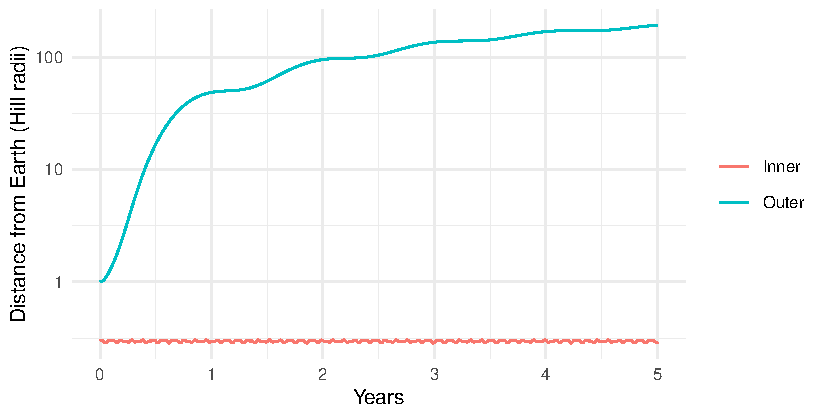
\includegraphics[width=1\linewidth,height=\textheight,keepaspectratio]{11-chaos-and-the-three-body-problem_files/figure-pdf/fig-hill-1.pdf}

}

\caption{\label{fig-hill}Two test moons of Earth, started on circular
orbits at 0.3 and 1.0 Hill radii. The inner one stays; the outer one is
stripped by the Sun within the first orbit.}

\end{figure}%

The inner moon's distance stays in a narrow band; the outer one wanders
off within months and is thereafter a planet in its own right, orbiting
the Sun near Earth. The Hill radius is the boundary of a planet's
domain, and it explains a great deal: why the giant planets, with
enormous Hill spheres, have dozens of moons each; why Mercury, deep in
the Sun's gravity, has none; and why the Moon's orbit, though perturbed
by the Sun in a hundred measurable ways, is in no danger.

\section{The Lagrange points, and which ones are
traps}\label{the-lagrange-points-and-which-ones-are-traps}

Chapter 10 found the \(L_4\) point, where a small body can orbit with
Jupiter indefinitely. There are five such points in the rotating frame
of any circular binary. \(L_1\) lies between the two bodies, \(L_2\)
beyond the smaller one, \(L_3\) beyond the larger one, and \(L_4\) and
\(L_5\) at the two equilateral positions. Only the last two are stable,
and only when the mass ratio is small. \(L_1\), \(L_2\), and \(L_3\) are
\emph{saddle points}: a body placed exactly there stays, but any
displacement along one direction grows exponentially.

\(L_1\) and \(L_2\) are at approximately one Hill radius from the
smaller body, toward and away from the larger one;
Equation~\ref{eq-hill} is in fact the leading-order position of those
two points. Put a test body at the Sun-Earth \(L_1\), moving so that it
would co-rotate with Earth, and watch:

\begin{Shaded}
\begin{Highlighting}[]
\NormalTok{d     }\OtherTok{\textless{}{-}}\NormalTok{ distance\_earth\_sun}
\NormalTok{omega }\OtherTok{\textless{}{-}} \FunctionTok{sqrt}\NormalTok{(gravitational\_constant }\SpecialCharTok{*}\NormalTok{ (mass\_sun }\SpecialCharTok{+}\NormalTok{ mass\_earth) }\SpecialCharTok{/}\NormalTok{ d}\SpecialCharTok{\^{}}\DecValTok{3}\NormalTok{)}
\NormalTok{M     }\OtherTok{\textless{}{-}}\NormalTok{ mass\_sun }\SpecialCharTok{+}\NormalTok{ mass\_earth}

\NormalTok{earth\_x }\OtherTok{\textless{}{-}}\NormalTok{ d }\SpecialCharTok{*}\NormalTok{ mass\_sun }\SpecialCharTok{/}\NormalTok{ M           }\CommentTok{\# Earth\textquotesingle{}s distance from the barycenter}
\NormalTok{L1      }\OtherTok{\textless{}{-}} \FunctionTok{c}\NormalTok{(earth\_x }\SpecialCharTok{{-}}\NormalTok{ r\_H, }\DecValTok{0}\NormalTok{)}
\NormalTok{v\_L1    }\OtherTok{\textless{}{-}}\NormalTok{ omega }\SpecialCharTok{*} \FunctionTok{c}\NormalTok{(}\SpecialCharTok{{-}}\NormalTok{L1[}\DecValTok{2}\NormalTok{], L1[}\DecValTok{1}\NormalTok{])}

\NormalTok{l1\_test }\OtherTok{\textless{}{-}} \FunctionTok{create\_system}\NormalTok{() }\SpecialCharTok{|\textgreater{}}
  \FunctionTok{add\_body}\NormalTok{(}\StringTok{"Sun"}\NormalTok{,   }\AttributeTok{mass =}\NormalTok{ mass\_sun,   }\AttributeTok{x =} \SpecialCharTok{{-}}\NormalTok{d }\SpecialCharTok{*}\NormalTok{ mass\_earth }\SpecialCharTok{/}\NormalTok{ M,}
           \AttributeTok{vy =} \SpecialCharTok{{-}}\NormalTok{omega }\SpecialCharTok{*}\NormalTok{ d }\SpecialCharTok{*}\NormalTok{ mass\_earth }\SpecialCharTok{/}\NormalTok{ M) }\SpecialCharTok{|\textgreater{}}
  \FunctionTok{add\_body}\NormalTok{(}\StringTok{"Earth"}\NormalTok{, }\AttributeTok{mass =}\NormalTok{ mass\_earth, }\AttributeTok{x =}\NormalTok{ earth\_x, }\AttributeTok{vy =}\NormalTok{ omega }\SpecialCharTok{*}\NormalTok{ earth\_x) }\SpecialCharTok{|\textgreater{}}
  \FunctionTok{add\_body}\NormalTok{(}\StringTok{"Probe"}\NormalTok{, }\AttributeTok{mass =} \FloatTok{1e3}\NormalTok{, }\AttributeTok{x =}\NormalTok{ L1[}\DecValTok{1}\NormalTok{], }\AttributeTok{vx =}\NormalTok{ v\_L1[}\DecValTok{1}\NormalTok{], }\AttributeTok{vy =}\NormalTok{ v\_L1[}\DecValTok{2}\NormalTok{]) }\SpecialCharTok{|\textgreater{}}
  \FunctionTok{simulate\_system}\NormalTok{(}\AttributeTok{time\_step =}\NormalTok{ seconds\_per\_hour, }\AttributeTok{duration =}\NormalTok{ seconds\_per\_year)}
\end{Highlighting}
\end{Shaded}

\begin{Shaded}
\begin{Highlighting}[]
\NormalTok{l1\_test }\SpecialCharTok{|\textgreater{}}
  \FunctionTok{filter}\NormalTok{(id }\SpecialCharTok{==} \StringTok{"Probe"}\NormalTok{) }\SpecialCharTok{|\textgreater{}}
  \FunctionTok{mutate}\NormalTok{(}\AttributeTok{theta =}\NormalTok{ omega }\SpecialCharTok{*}\NormalTok{ time,}
         \AttributeTok{xr =}\NormalTok{  x }\SpecialCharTok{*} \FunctionTok{cos}\NormalTok{(theta) }\SpecialCharTok{+}\NormalTok{ y }\SpecialCharTok{*} \FunctionTok{sin}\NormalTok{(theta),}
         \AttributeTok{yr =} \SpecialCharTok{{-}}\NormalTok{x }\SpecialCharTok{*} \FunctionTok{sin}\NormalTok{(theta) }\SpecialCharTok{+}\NormalTok{ y }\SpecialCharTok{*} \FunctionTok{cos}\NormalTok{(theta),}
         \AttributeTok{displacement =} \FunctionTok{sqrt}\NormalTok{((xr }\SpecialCharTok{{-}}\NormalTok{ L1[}\DecValTok{1}\NormalTok{])}\SpecialCharTok{\^{}}\DecValTok{2} \SpecialCharTok{+}\NormalTok{ (yr }\SpecialCharTok{{-}}\NormalTok{ L1[}\DecValTok{2}\NormalTok{])}\SpecialCharTok{\^{}}\DecValTok{2}\NormalTok{)) }\SpecialCharTok{|\textgreater{}}
  \FunctionTok{ggplot}\NormalTok{(}\FunctionTok{aes}\NormalTok{(time }\SpecialCharTok{/}\NormalTok{ seconds\_per\_day, displacement }\SpecialCharTok{/} \FloatTok{1e3}\NormalTok{)) }\SpecialCharTok{+}
  \FunctionTok{geom\_line}\NormalTok{() }\SpecialCharTok{+}
  \FunctionTok{scale\_y\_log10}\NormalTok{() }\SpecialCharTok{+}
  \FunctionTok{labs}\NormalTok{(}\AttributeTok{x =} \StringTok{"Day"}\NormalTok{, }\AttributeTok{y =} \StringTok{"Displacement from L1 (km)"}\NormalTok{)}
\end{Highlighting}
\end{Shaded}

\begin{figure}[tbp]

\centering{

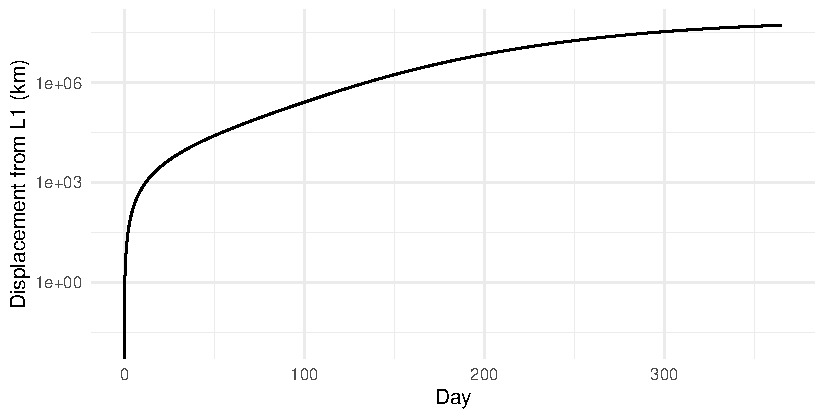
\includegraphics[width=1\linewidth,height=\textheight,keepaspectratio]{11-chaos-and-the-three-body-problem_files/figure-pdf/fig-l1-1.pdf}

}

\caption{\label{fig-l1}A probe placed at the Sun-Earth \(L_1\) point.
Its displacement from \(L_1\) in the rotating frame grows exponentially
with an e-folding time of a few weeks.}

\end{figure}%

\begin{Shaded}
\begin{Highlighting}[]
\NormalTok{l1\_growth }\OtherTok{\textless{}{-}}\NormalTok{ l1\_test }\SpecialCharTok{|\textgreater{}}
  \FunctionTok{filter}\NormalTok{(id }\SpecialCharTok{==} \StringTok{"Probe"}\NormalTok{) }\SpecialCharTok{|\textgreater{}}
  \FunctionTok{mutate}\NormalTok{(}\AttributeTok{theta =}\NormalTok{ omega }\SpecialCharTok{*}\NormalTok{ time,}
         \AttributeTok{xr =}\NormalTok{  x }\SpecialCharTok{*} \FunctionTok{cos}\NormalTok{(theta) }\SpecialCharTok{+}\NormalTok{ y }\SpecialCharTok{*} \FunctionTok{sin}\NormalTok{(theta),}
         \AttributeTok{yr =} \SpecialCharTok{{-}}\NormalTok{x }\SpecialCharTok{*} \FunctionTok{sin}\NormalTok{(theta) }\SpecialCharTok{+}\NormalTok{ y }\SpecialCharTok{*} \FunctionTok{cos}\NormalTok{(theta),}
         \AttributeTok{displacement =} \FunctionTok{sqrt}\NormalTok{((xr }\SpecialCharTok{{-}}\NormalTok{ L1[}\DecValTok{1}\NormalTok{])}\SpecialCharTok{\^{}}\DecValTok{2} \SpecialCharTok{+}\NormalTok{ (yr }\SpecialCharTok{{-}}\NormalTok{ L1[}\DecValTok{2}\NormalTok{])}\SpecialCharTok{\^{}}\DecValTok{2}\NormalTok{)) }\SpecialCharTok{|\textgreater{}}
  \FunctionTok{filter}\NormalTok{(time }\SpecialCharTok{\textgreater{}}\NormalTok{ seconds\_per\_day }\SpecialCharTok{*} \DecValTok{20}\NormalTok{, time }\SpecialCharTok{\textless{}}\NormalTok{ seconds\_per\_day }\SpecialCharTok{*} \DecValTok{120}\NormalTok{)}

\DecValTok{1} \SpecialCharTok{/} \FunctionTok{coef}\NormalTok{(}\FunctionTok{lm}\NormalTok{(}\FunctionTok{log}\NormalTok{(displacement) }\SpecialCharTok{\textasciitilde{}}\NormalTok{ time, }\AttributeTok{data =}\NormalTok{ l1\_growth))[[}\StringTok{"time"}\NormalTok{]] }\SpecialCharTok{/}\NormalTok{ seconds\_per\_day}
\CommentTok{\#\textgreater{} [1] 19.98168}
\end{Highlighting}
\end{Shaded}

The e-folding time is a few weeks. (The probe does not start exactly at
\(L_1\), because Equation~\ref{eq-hill} is only the first term of the
exact position, so it begins drifting at once; a body placed with
perfect precision would still be dislodged by the Moon, the other
planets, and sunlight.) This is why the spacecraft parked at \(L_1\) and
\(L_2\), SOHO, Gaia, JWST, do not sit at the point but fly \emph{halo
orbits} around it, and fire their thrusters every few weeks to stay on
them. The instability is slow enough to manage and fast enough that it
can never be ignored.

\begin{tcolorbox}[enhanced jigsaw, arc=.35mm, bottomrule=.15mm, bottomtitle=1mm, breakable, colback=white, colbacktitle=quarto-callout-tip-color!10!white, colframe=quarto-callout-tip-color-frame, coltitle=black, left=2mm, leftrule=.75mm, opacityback=0, opacitybacktitle=0.6, rightrule=.15mm, title={Key results}, titlerule=0mm, toprule=.15mm, toptitle=1mm]

\begin{itemize}
\tightlist
\item
  Nearby trajectories of a chaotic system separate as \(e^{t/\tau}\);
  \(\tau\) is the Lyapunov time. Beyond a few \(\tau\), a simulation
  predicts the statistics of the motion, not the motion.
\item
  A body has escaped when its energy relative to the rest of the system
  is positive. Three-body breakups eject one body and leave a tighter,
  more eccentric binary. Total energy is conserved throughout.
\item
  Hierarchical triples are stable. The Hill radius
  \(r_{\mathrm{H}} = R\,(m/3M)^{1/3}\) bounds a planet's domain;
  prograde satellites survive out to about half of it.
\item
  \(L_1\), \(L_2\), \(L_3\) are unstable saddle points with e-folding
  times of weeks (Sun-Earth); \(L_4\), \(L_5\) are stable for small mass
  ratios.
\end{itemize}

\end{tcolorbox}

\chapter{Conservation Laws as Diagnostics}\label{sec-diagnostics}

A simulation can be wrong in ways that are invisible in a plot. An orbit
that is an ellipse of the right size, traced at the right speed, can
still be rotating slowly in its plane for no physical reason, and
nothing about the picture will tell you. What \emph{will} tell you is a
set of quantities that the real system keeps constant and the simulated
one may not. Chapter 5 used total energy this way; this chapter adds
total momentum and total angular momentum, derives why all three are
conserved for any number of bodies, explains which of them a good
integrator conserves \emph{exactly} and which only approximately, and
turns them into a single function you can run on any simulation output.
It ends with a worked diagnosis of a simulation that passes the energy
test and is still wrong.

\section{\texorpdfstring{Three conserved quantities, for \(N\)
bodies}{Three conserved quantities, for N bodies}}\label{three-conserved-quantities-for-n-bodies}

Chapter 4 derived conservation of energy and angular momentum for two
bodies. The \(N\)-body versions follow from two properties of gravity:
it is \emph{pairwise antisymmetric}
(\(\mathbf{F}_{jk} = -\mathbf{F}_{kj}\)) and \emph{central}
(\(\mathbf{F}_{jk}\) lies along \(\mathbf{r}_k - \mathbf{r}_j\)).

\textbf{Momentum.} \(\mathbf{P} = \sum_j m_j\mathbf{v}_j\), and

\[
\dot{\mathbf{P}} = \sum_j m_j\mathbf{a}_j = \sum_j\sum_{k\ne j}\mathbf{F}_{jk} = \sum_{j<k}\left(\mathbf{F}_{jk} + \mathbf{F}_{kj}\right) = \mathbf{0}.
\]

Every force appears twice with opposite signs. The center of mass moves
in a straight line at constant velocity, which is Chapter 2's drifting
Earth.

\textbf{Angular momentum.}
\(\mathbf{L} = \sum_j m_j\,\mathbf{r}_j\times\mathbf{v}_j\), and since
\(\mathbf{v}_j\times\mathbf{v}_j = 0\),

\[
\dot{\mathbf{L}} = \sum_j \mathbf{r}_j\times m_j\mathbf{a}_j = \sum_{j<k}\left(\mathbf{r}_j\times\mathbf{F}_{jk} + \mathbf{r}_k\times\mathbf{F}_{kj}\right) = \sum_{j<k}\left(\mathbf{r}_j - \mathbf{r}_k\right)\times\mathbf{F}_{jk} = \mathbf{0},
\]

because \(\mathbf{F}_{jk}\) is parallel to
\(\mathbf{r}_j - \mathbf{r}_k\). Antisymmetry collapses the two terms of
each pair into one; centrality kills it.

\textbf{Energy.}
\(E = \sum_j \tfrac12 m_j v_j^2 - \sum_{j<k} G m_j m_k/r_{jk}\)
(Equation~\ref{eq-total-energy}). The kinetic term's rate of change is
\(\sum_j m_j\mathbf{v}_j\cdot\mathbf{a}_j = \sum_{j<k}\mathbf{F}_{jk}\cdot(\mathbf{v}_j - \mathbf{v}_k)\),
again by antisymmetry. With
\(\mathbf{F}_{jk} = G m_j m_k(\mathbf{r}_k - \mathbf{r}_j)/r_{jk}^3\)
and the identity
\((\mathbf{r}_k - \mathbf{r}_j)\cdot(\mathbf{v}_k - \mathbf{v}_j) = r_{jk}\dot r_{jk}\)
from Chapter 4,

\[
\mathbf{F}_{jk}\cdot(\mathbf{v}_j - \mathbf{v}_k) = -\frac{G m_j m_k\,\dot r_{jk}}{r_{jk}^2},
\]

and the potential term's rate of change is
\(\sum_{j<k} G m_j m_k\,\dot r_{jk}/r_{jk}^2\), which cancels it pair by
pair. With softening (Chapter 6), replace \(r_{jk}\) by
\(\sqrt{r_{jk}^2+\varepsilon^2}\) in the potential and the same
cancellation goes through.

\begin{tcolorbox}[enhanced jigsaw, arc=.35mm, bottomrule=.15mm, bottomtitle=1mm, breakable, colback=white, colbacktitle=quarto-callout-note-color!10!white, colframe=quarto-callout-note-color-frame, coltitle=black, left=2mm, leftrule=.75mm, opacityback=0, opacitybacktitle=0.6, rightrule=.15mm, title={Where it comes from}, titlerule=0mm, toprule=.15mm, toptitle=1mm]

Each of the three laws is the shadow of a symmetry. Emmy Noether proved
in 1918 that every continuous symmetry of a physical system's equations
gives a conserved quantity: invariance under translation in space gives
momentum, under rotation gives angular momentum, under translation in
\emph{time} gives energy. The N-body equations have all three
symmetries, so they have all three laws.

A numerical integrator does not have all three. A fixed-step scheme
respects translations and rotations perfectly: shift or rotate every
position and velocity, run a step, and you get the shifted or rotated
result, exactly. But it does not respect translation in time, because
time comes in lumps of \(\Delta t\). Noether's theorem then says exactly
what to expect: a well-constructed integrator conserves momentum and
angular momentum to rounding error, but energy only approximately. That
is what the next section finds.

\end{tcolorbox}

\section{Which laws an integrator keeps
exactly}\label{which-laws-an-integrator-keeps-exactly}

Look at the integrators of Chapter 5 as compositions of \emph{kicks}
(velocity updates from accelerations computed at fixed positions) and
\emph{drifts} (position updates at fixed velocities).

A kick changes \(\mathbf{P}\) by
\(\Delta t\sum_j m_j\mathbf{a}_j = \Delta t\sum_j\mathbf{F}_j = \mathbf{0}\)
and \(\mathbf{L}\) by
\(\Delta t\sum_j\mathbf{r}_j\times m_j\mathbf{a}_j = \mathbf{0}\), by
the same pairwise arguments as above, \emph{exactly}, for any
\(\Delta t\). A drift changes neither: \(\mathbf{P}\) does not involve
positions, and \(\mathbf{L}\) changes by
\(\Delta t\sum_j m_j\mathbf{v}_j\times\mathbf{v}_j = \mathbf{0}\). So
any method that is a sequence of kicks and drifts, which is Euler-Cromer
(kick, drift) and Velocity Verlet (half kick, drift, half kick),
conserves momentum and angular momentum to machine precision no matter
how large the step.

Plain Euler is not a kick followed by a drift; it updates positions with
the \emph{old} velocities and velocities with the \emph{old}
accelerations simultaneously. Momentum still survives, but angular
momentum picks up \(\Delta t^2\sum_j m_j\mathbf{v}_j\times\mathbf{a}_j\)
per step, which does not vanish. So the three laws grade the three
methods differently:

\begin{longtable}[]{@{}
  >{\raggedright\arraybackslash}p{(\linewidth - 6\tabcolsep) * \real{0.2500}}
  >{\raggedright\arraybackslash}p{(\linewidth - 6\tabcolsep) * \real{0.2500}}
  >{\raggedright\arraybackslash}p{(\linewidth - 6\tabcolsep) * \real{0.2500}}
  >{\raggedright\arraybackslash}p{(\linewidth - 6\tabcolsep) * \real{0.2500}}@{}}
\caption{What each integrator conserves (exact means to rounding
error).}\label{tbl-conservation}\tabularnewline
\toprule\noalign{}
\begin{minipage}[b]{\linewidth}\raggedright
\end{minipage} & \begin{minipage}[b]{\linewidth}\raggedright
Euler
\end{minipage} & \begin{minipage}[b]{\linewidth}\raggedright
Euler-Cromer
\end{minipage} & \begin{minipage}[b]{\linewidth}\raggedright
Verlet
\end{minipage} \\
\midrule\noalign{}
\endfirsthead
\toprule\noalign{}
\begin{minipage}[b]{\linewidth}\raggedright
\end{minipage} & \begin{minipage}[b]{\linewidth}\raggedright
Euler
\end{minipage} & \begin{minipage}[b]{\linewidth}\raggedright
Euler-Cromer
\end{minipage} & \begin{minipage}[b]{\linewidth}\raggedright
Verlet
\end{minipage} \\
\midrule\noalign{}
\endhead
\bottomrule\noalign{}
\endlastfoot
Momentum & exact & exact & exact \\
Angular momentum & \(O(\Delta t)\) drift & exact & exact \\
Energy & \(O(\Delta t)\) drift & bounded, \(O(\Delta t)\) & bounded,
\(O(\Delta t^2)\) \\
\end{longtable}

The table is the key to reading diagnostics. A momentum or angular
momentum error that grows past rounding in a Verlet run is not a
time-step problem; it is a bug, in your setup or in the code. An energy
error is a time-step problem (or an integrator problem), and its
\emph{shape} says which.

\section{Computing all three}\label{computing-all-three}

The package has one function per quantity, and each is a single grouped
sum over the output tibble. Chapter 5 wrote out the energy; momentum and
angular momentum are shorter still, and this is all
\texttt{get\_momentum()} and \texttt{get\_angular\_momentum()} do:

\begin{Shaded}
\begin{Highlighting}[]
\NormalTok{sim }\SpecialCharTok{|\textgreater{}}
  \FunctionTok{group\_by}\NormalTok{(time) }\SpecialCharTok{|\textgreater{}}
  \FunctionTok{summarise}\NormalTok{(}\AttributeTok{px =} \FunctionTok{sum}\NormalTok{(mass }\SpecialCharTok{*}\NormalTok{ vx), }\AttributeTok{py =} \FunctionTok{sum}\NormalTok{(mass }\SpecialCharTok{*}\NormalTok{ vy), }\AttributeTok{pz =} \FunctionTok{sum}\NormalTok{(mass }\SpecialCharTok{*}\NormalTok{ vz))}

\NormalTok{sim }\SpecialCharTok{|\textgreater{}}
  \FunctionTok{group\_by}\NormalTok{(time) }\SpecialCharTok{|\textgreater{}}
  \FunctionTok{summarise}\NormalTok{(}\AttributeTok{Lx =} \FunctionTok{sum}\NormalTok{(mass }\SpecialCharTok{*}\NormalTok{ (y }\SpecialCharTok{*}\NormalTok{ vz }\SpecialCharTok{{-}}\NormalTok{ z }\SpecialCharTok{*}\NormalTok{ vy)),}
            \AttributeTok{Ly =} \FunctionTok{sum}\NormalTok{(mass }\SpecialCharTok{*}\NormalTok{ (z }\SpecialCharTok{*}\NormalTok{ vx }\SpecialCharTok{{-}}\NormalTok{ x }\SpecialCharTok{*}\NormalTok{ vz)),}
            \AttributeTok{Lz =} \FunctionTok{sum}\NormalTok{(mass }\SpecialCharTok{*}\NormalTok{ (x }\SpecialCharTok{*}\NormalTok{ vy }\SpecialCharTok{{-}}\NormalTok{ y }\SpecialCharTok{*}\NormalTok{ vx)))}
\end{Highlighting}
\end{Shaded}

\texttt{conserved\_quantities()} joins the three into one tidy time
series and adds the relative errors. For energy that is
\((E - E_0)/|E_0|\) as before. Momentum is often exactly zero at the
start, so its error is measured against the total
\(\sum_j m_j|\mathbf{v}_j|\) at \(t = 0\) instead; angular momentum
against \(|\mathbf{L}_0|\). On Chapter 5's star and planet with the
three methods:

\begin{Shaded}
\begin{Highlighting}[]
\NormalTok{star\_planet }\OtherTok{\textless{}{-}} \FunctionTok{create\_system}\NormalTok{() }\SpecialCharTok{|\textgreater{}}
  \FunctionTok{add\_body}\NormalTok{(}\StringTok{"Star"}\NormalTok{,   }\AttributeTok{mass =} \FloatTok{1e30}\NormalTok{) }\SpecialCharTok{|\textgreater{}}
  \FunctionTok{add\_body}\NormalTok{(}\StringTok{"Planet"}\NormalTok{, }\AttributeTok{mass =} \FloatTok{1e24}\NormalTok{, }\AttributeTok{x =} \FloatTok{1e11}\NormalTok{, }\AttributeTok{vy =} \DecValTok{30000}\NormalTok{)}

\NormalTok{runs }\OtherTok{\textless{}{-}} \FunctionTok{bind\_rows}\NormalTok{(}\FunctionTok{lapply}\NormalTok{(}\FunctionTok{c}\NormalTok{(}\StringTok{"verlet"}\NormalTok{, }\StringTok{"euler\_cromer"}\NormalTok{, }\StringTok{"euler"}\NormalTok{), }\ControlFlowTok{function}\NormalTok{(m) \{}
\NormalTok{  star\_planet }\SpecialCharTok{|\textgreater{}}
    \FunctionTok{simulate\_system}\NormalTok{(}\AttributeTok{time\_step =}\NormalTok{ seconds\_per\_hour }\SpecialCharTok{*} \DecValTok{6}\NormalTok{,}
                    \AttributeTok{duration =}\NormalTok{ seconds\_per\_year }\SpecialCharTok{*} \DecValTok{10}\NormalTok{, }\AttributeTok{method =}\NormalTok{ m) }\SpecialCharTok{|\textgreater{}}
    \FunctionTok{conserved\_quantities}\NormalTok{() }\SpecialCharTok{|\textgreater{}}
    \FunctionTok{mutate}\NormalTok{(}\AttributeTok{method =}\NormalTok{ m)}
\NormalTok{\}))}
\end{Highlighting}
\end{Shaded}

\begin{Shaded}
\begin{Highlighting}[]
\NormalTok{runs }\SpecialCharTok{|\textgreater{}}
  \FunctionTok{select}\NormalTok{(time, method, energy\_error, momentum\_error, angular\_momentum\_error) }\SpecialCharTok{|\textgreater{}}
\NormalTok{  tidyr}\SpecialCharTok{::}\FunctionTok{pivot\_longer}\NormalTok{(}\FunctionTok{c}\NormalTok{(energy\_error, momentum\_error, angular\_momentum\_error),}
                      \AttributeTok{names\_to =} \StringTok{"quantity"}\NormalTok{, }\AttributeTok{values\_to =} \StringTok{"error"}\NormalTok{) }\SpecialCharTok{|\textgreater{}}
  \FunctionTok{mutate}\NormalTok{(}\AttributeTok{quantity =} \FunctionTok{sub}\NormalTok{(}\StringTok{"\_error$"}\NormalTok{, }\StringTok{""}\NormalTok{, quantity)) }\SpecialCharTok{|\textgreater{}}
  \FunctionTok{ggplot}\NormalTok{(}\FunctionTok{aes}\NormalTok{(time }\SpecialCharTok{/}\NormalTok{ seconds\_per\_year, error)) }\SpecialCharTok{+}
  \FunctionTok{geom\_line}\NormalTok{() }\SpecialCharTok{+}
  \FunctionTok{facet\_grid}\NormalTok{(quantity }\SpecialCharTok{\textasciitilde{}}\NormalTok{ method, }\AttributeTok{scales =} \StringTok{"free\_y"}\NormalTok{) }\SpecialCharTok{+}
  \FunctionTok{labs}\NormalTok{(}\AttributeTok{x =} \StringTok{"Years"}\NormalTok{, }\AttributeTok{y =} \StringTok{"Relative error"}\NormalTok{)}
\end{Highlighting}
\end{Shaded}

\begin{figure}[tbp]

\centering{

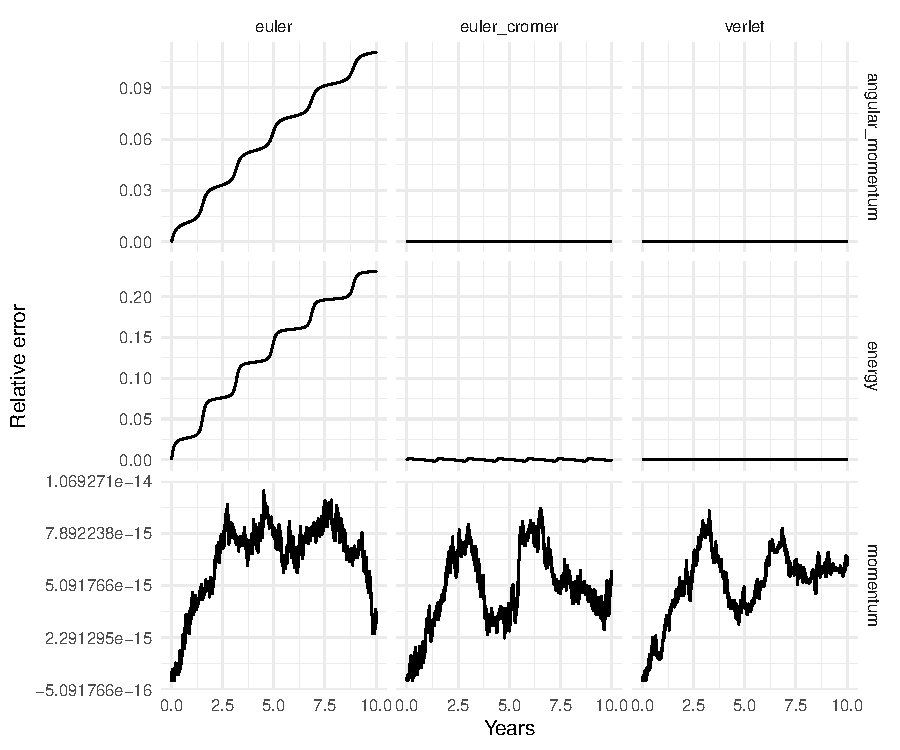
\includegraphics[width=1\linewidth,height=\textheight,keepaspectratio]{12-energy-and-angular-momentum_files/figure-pdf/fig-diagnostics-1.pdf}

}

\caption{\label{fig-diagnostics}Relative errors in energy, momentum, and
angular momentum for ten years of the same orbit with three integrators.
Momentum is conserved to rounding by all three; angular momentum by the
two symplectic methods; energy by none, but Verlet's error stays in a
narrow band. Note the free vertical scales.}

\end{figure}%

Every panel in the table above has its picture here. The momentum row is
noise at the \(10^{-16}\) level for all three methods. The angular
momentum row is noise for Verlet and Euler-Cromer and a steady climb for
Euler. The energy row is Chapter 5's figure again.

\section{Reading the plots}\label{reading-the-plots}

Four shapes cover nearly everything you will see in an energy
diagnostic.

\textbf{A narrow band, oscillating with the orbit.} Healthy. The band's
width is the integrator's \(O(\Delta t^2)\) error and halving the step
should shrink it by four. Nothing to do.

\textbf{A wide band, still oscillating.} The step is too large for the
tightest or most eccentric orbit in the system. The run is probably not
catastrophically wrong, but the next section shows that ``bounded energy
error'' is a weaker guarantee than it sounds. Halve the step and
compare.

\textbf{A steady drift.} Either the wrong integrator (Euler), or a step
so large that the symplectic integrator's shadow-Hamiltonian guarantee
has broken down, which happens when \(\Delta t\) approaches the
periapsis timescale of some orbit (Chapter 13). Check \texttt{method},
then halve the step.

\textbf{A sudden jump.} A close encounter. Two bodies passed each other
faster than the step could follow and the integrator handed one of them
a spurious kick (Chapter 6). Everything after the jump is on a different
orbit from everything before. Either the encounter needs a smaller step
(Chapter 13's segmented runs) or it is a collision in disguise and the
simulation should not continue past it.

A fifth shape is an apparent drift that is not real: you ran with
\texttt{softening} and computed the energy without it. The softened
force conserves the softened energy; \texttt{conserved\_quantities()}
reads the softening length from the run, so this only bites if you
compute the energy by hand or override the argument.

\section{A worked diagnosis: the orbit that looked
fine}\label{a-worked-diagnosis-the-orbit-that-looked-fine}

Mercury's perihelion precesses by 574 arcseconds per century, of which
531 come from the other planets and 43 from general relativity. Suppose
you wanted to measure the planetary part with orbitr. The first question
is what the integrator does to Mercury's perihelion when there are
\emph{no} other planets, where the correct answer is zero precession.
Two bodies, ten years, with daily and five-day steps:

\begin{Shaded}
\begin{Highlighting}[]
\NormalTok{mercury\_run }\OtherTok{\textless{}{-}} \ControlFlowTok{function}\NormalTok{(step\_days) \{}
  \FunctionTok{create\_system}\NormalTok{() }\SpecialCharTok{|\textgreater{}}
    \FunctionTok{add\_sun}\NormalTok{() }\SpecialCharTok{|\textgreater{}}
    \FunctionTok{add\_planet}\NormalTok{(}\StringTok{"Mercury"}\NormalTok{, }\AttributeTok{parent =} \StringTok{"Sun"}\NormalTok{) }\SpecialCharTok{|\textgreater{}}
    \FunctionTok{simulate\_system}\NormalTok{(}\AttributeTok{time\_step =}\NormalTok{ seconds\_per\_day }\SpecialCharTok{*}\NormalTok{ step\_days,}
                    \AttributeTok{duration =}\NormalTok{ seconds\_per\_year }\SpecialCharTok{*} \DecValTok{10}\NormalTok{)}
\NormalTok{\}}

\NormalTok{perihelion\_angle }\OtherTok{\textless{}{-}} \ControlFlowTok{function}\NormalTok{(sim) \{}
  \CommentTok{\# longitude of perihelion = node + argument of perihelion, unwrapped so it}
  \CommentTok{\# can be tracked through 360 degrees}
  \FunctionTok{get\_orbital\_elements}\NormalTok{(sim, }\StringTok{"Mercury"}\NormalTok{, }\StringTok{"Sun"}\NormalTok{) }\SpecialCharTok{|\textgreater{}}
    \FunctionTok{mutate}\NormalTok{(}\AttributeTok{omega\_deg =} \FunctionTok{unwrap}\NormalTok{((lan }\SpecialCharTok{+}\NormalTok{ arg\_pe) }\SpecialCharTok{*}\NormalTok{ pi }\SpecialCharTok{/} \DecValTok{180}\NormalTok{) }\SpecialCharTok{*} \DecValTok{180} \SpecialCharTok{/}\NormalTok{ pi) }\SpecialCharTok{|\textgreater{}}
    \FunctionTok{select}\NormalTok{(time, omega\_deg)}
\NormalTok{\}}

\NormalTok{runs\_m }\OtherTok{\textless{}{-}} \FunctionTok{bind\_rows}\NormalTok{(}\FunctionTok{lapply}\NormalTok{(}\FunctionTok{c}\NormalTok{(}\DecValTok{5}\NormalTok{, }\DecValTok{2}\NormalTok{, }\DecValTok{1}\NormalTok{), }\ControlFlowTok{function}\NormalTok{(s) \{}
\NormalTok{  sim }\OtherTok{\textless{}{-}} \FunctionTok{mercury\_run}\NormalTok{(s)}
  \FunctionTok{perihelion\_angle}\NormalTok{(sim) }\SpecialCharTok{|\textgreater{}}
    \FunctionTok{mutate}\NormalTok{(}\AttributeTok{step\_days =}\NormalTok{ s,}
           \AttributeTok{energy\_error =} \FunctionTok{conserved\_quantities}\NormalTok{(sim)}\SpecialCharTok{$}\NormalTok{energy\_error)}
\NormalTok{\}))}
\end{Highlighting}
\end{Shaded}

(The longitude of perihelion, \(\Omega + \omega\), is the quantity to
track rather than \(\omega\) alone, because for Mercury's small
inclination the node is poorly defined and the two angles can trade
against each other while their sum stays put.)

\begin{Shaded}
\begin{Highlighting}[]
\FunctionTok{bind\_rows}\NormalTok{(}
\NormalTok{  runs\_m }\SpecialCharTok{|\textgreater{}} \FunctionTok{group\_by}\NormalTok{(step\_days) }\SpecialCharTok{|\textgreater{}}
    \FunctionTok{transmute}\NormalTok{(time, }\AttributeTok{panel =} \StringTok{"Perihelion direction (deg)"}\NormalTok{,}
              \AttributeTok{value =}\NormalTok{ omega\_deg }\SpecialCharTok{{-}} \FunctionTok{first}\NormalTok{(omega\_deg)),}
\NormalTok{  runs\_m }\SpecialCharTok{|\textgreater{}} \FunctionTok{group\_by}\NormalTok{(step\_days) }\SpecialCharTok{|\textgreater{}}
    \FunctionTok{transmute}\NormalTok{(time, }\AttributeTok{panel =} \StringTok{"Relative energy error"}\NormalTok{, }\AttributeTok{value =}\NormalTok{ energy\_error)}
\NormalTok{) }\SpecialCharTok{|\textgreater{}}
  \FunctionTok{ungroup}\NormalTok{() }\SpecialCharTok{|\textgreater{}}
  \FunctionTok{ggplot}\NormalTok{(}\FunctionTok{aes}\NormalTok{(time }\SpecialCharTok{/}\NormalTok{ seconds\_per\_year, value, }\AttributeTok{color =} \FunctionTok{factor}\NormalTok{(step\_days))) }\SpecialCharTok{+}
  \FunctionTok{geom\_line}\NormalTok{() }\SpecialCharTok{+}
  \FunctionTok{facet\_wrap}\NormalTok{(}\SpecialCharTok{\textasciitilde{}}\NormalTok{ panel, }\AttributeTok{scales =} \StringTok{"free\_y"}\NormalTok{) }\SpecialCharTok{+}
  \FunctionTok{labs}\NormalTok{(}\AttributeTok{x =} \StringTok{"Years"}\NormalTok{, }\AttributeTok{y =} \ConstantTok{NULL}\NormalTok{, }\AttributeTok{color =} \StringTok{"Step (days)"}\NormalTok{)}
\end{Highlighting}
\end{Shaded}

\begin{figure}[tbp]

\centering{

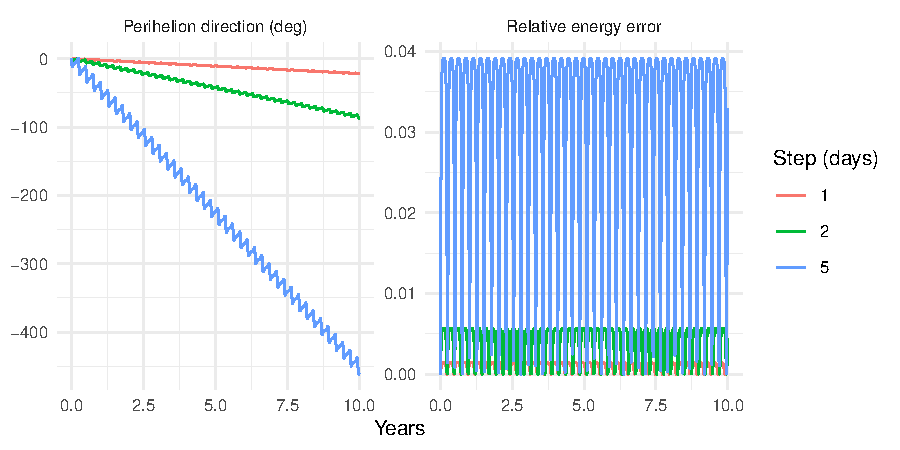
\includegraphics[width=1\linewidth,height=\textheight,keepaspectratio]{12-energy-and-angular-momentum_files/figure-pdf/fig-spurious-precession-1.pdf}

}

\caption{\label{fig-spurious-precession}Left: Mercury's perihelion
direction in a two-body run, which should be a flat line, at three step
sizes. Right: the energy error of the same runs, which is bounded in
every case. Bounded energy did not prevent the orbit from rotating.}

\end{figure}%

The energy error is bounded at every step size, exactly as advertised.
And the perihelion of the five-day run rotates through tens of degrees
in a decade, for no physical reason at all. The daily run rotates too,
more slowly. This is \emph{numerical precession}: the integrator's
shadow Hamiltonian is not Kepler's, and the difference, though it
conserves energy, does not conserve the eccentricity vector. It is the
single most common artifact in orbital simulation, and the energy test
is blind to it.

Measure the rate at each step:

\begin{Shaded}
\begin{Highlighting}[]
\NormalTok{rates }\OtherTok{\textless{}{-}}\NormalTok{ runs\_m }\SpecialCharTok{|\textgreater{}}
  \FunctionTok{group\_by}\NormalTok{(step\_days) }\SpecialCharTok{|\textgreater{}}
  \FunctionTok{summarise}\NormalTok{(}\AttributeTok{deg\_per\_year =} \FunctionTok{coef}\NormalTok{(}\FunctionTok{lm}\NormalTok{(omega\_deg }\SpecialCharTok{\textasciitilde{}} \FunctionTok{I}\NormalTok{(time }\SpecialCharTok{/}\NormalTok{ seconds\_per\_year)))[[}\DecValTok{2}\NormalTok{]])}
\NormalTok{rates}
\CommentTok{\#\textgreater{} \# A tibble: 3 x 2}
\CommentTok{\#\textgreater{}   step\_days deg\_per\_year}
\CommentTok{\#\textgreater{}       \textless{}dbl\textgreater{}        \textless{}dbl\textgreater{}}
\CommentTok{\#\textgreater{} 1         1        {-}2.18}
\CommentTok{\#\textgreater{} 2         2        {-}8.49}
\CommentTok{\#\textgreater{} 3         5       {-}45.1}
\end{Highlighting}
\end{Shaded}

Halving the step cuts the rate by about four: the artifact is
\(O(\Delta t^2)\), like everything else about Verlet. That scaling is
also the cure, because it lets you extrapolate. The real planetary
precession is \(531''\) per century, or \(0.0015°\) per year. To get the
artifact ten times smaller than the signal you would need a step of
about

\begin{Shaded}
\begin{Highlighting}[]
\NormalTok{rate\_1d }\OtherTok{\textless{}{-}}\NormalTok{ rates}\SpecialCharTok{$}\NormalTok{deg\_per\_year[rates}\SpecialCharTok{$}\NormalTok{step\_days }\SpecialCharTok{==} \DecValTok{1}\NormalTok{]}
\NormalTok{target  }\OtherTok{\textless{}{-}} \FloatTok{0.0015} \SpecialCharTok{/} \DecValTok{10}
\FunctionTok{sqrt}\NormalTok{(target }\SpecialCharTok{/} \FunctionTok{abs}\NormalTok{(rate\_1d)) }\SpecialCharTok{*} \DecValTok{24}          \CommentTok{\# hours}
\CommentTok{\#\textgreater{} [1] 0.1992759}
\end{Highlighting}
\end{Shaded}

hours. That is a smaller step than anyone would guess from looking at
the orbit, and it is what Chapter 8's last exercise was getting at when
it asked what limits the precision. The general lesson is worth stating
plainly: an energy diagnostic tells you the integrator is stable. It
does not tell you the integrator is accurate. For accuracy, find a
quantity the true dynamics conserves that the integrator does not, the
eccentricity vector is the usual one, and watch that.

\begin{tcolorbox}[enhanced jigsaw, arc=.35mm, bottomrule=.15mm, bottomtitle=1mm, breakable, colback=white, colbacktitle=quarto-callout-tip-color!10!white, colframe=quarto-callout-tip-color-frame, coltitle=black, left=2mm, leftrule=.75mm, opacityback=0, opacitybacktitle=0.6, rightrule=.15mm, title={Key results}, titlerule=0mm, toprule=.15mm, toptitle=1mm]

\begin{itemize}
\tightlist
\item
  \(N\)-body gravity conserves \(\mathbf{P}\), \(\mathbf{L}\), and \(E\)
  because it is pairwise antisymmetric, central, and derived from a
  potential.
\item
  Kick-drift integrators (Euler-Cromer, Verlet) conserve \(\mathbf{P}\)
  and \(\mathbf{L}\) to rounding error at any step size; a drift in
  either means a bug. Energy is conserved only approximately, and the
  shape of its error says what is wrong.
\item
  Bounded energy error does not imply an accurate orbit. Numerical
  precession of the periapsis is \(O(\Delta t^2)\) and invisible to the
  energy test; track the eccentricity vector.
\end{itemize}

\end{tcolorbox}

\chapter{Comets and Highly Eccentric Orbits}\label{sec-comets}

Everything in the solar system chapter was nearly circular, and nearly
circular orbits are easy: the speed hardly changes, so one time step is
as good as another. A comet is the opposite case. Halley's Comet spends
seventy years crawling through the outer solar system and a few months
sprinting around the Sun at sixty times the speed, and a step that is
wasteful at aphelion is hopeless at perihelion. This chapter sets Halley
up from its orbital elements, shows exactly how and where a fixed step
fails on it, and then builds the tool the package does not have: a way
to take small steps only when they are needed. It closes with two orbits
that are not ellipses at all.

\section{Halley}\label{halley}

Halley's Comet has semi-major axis 17.8 AU, eccentricity 0.967, and an
inclination of 162°, which is to say it orbits the Sun \emph{backward},
tilted 18° from the ecliptic. Its perihelion is 0.586 AU, inside Venus's
orbit; its aphelion is 35 AU, beyond Neptune's. Chapter 7's conversion
handles all of that:

\begin{Shaded}
\begin{Highlighting}[]
\NormalTok{AU     }\OtherTok{\textless{}{-}}\NormalTok{ distance\_earth\_sun}
\NormalTok{mu\_sun }\OtherTok{\textless{}{-}}\NormalTok{ gravitational\_constant }\SpecialCharTok{*}\NormalTok{ mass\_sun}

\NormalTok{halley }\OtherTok{\textless{}{-}} \FunctionTok{list}\NormalTok{(}\AttributeTok{a =} \FloatTok{17.834} \SpecialCharTok{*}\NormalTok{ AU, }\AttributeTok{e =} \FloatTok{0.96714}\NormalTok{, }\AttributeTok{i =} \FloatTok{162.26}\NormalTok{,}
               \AttributeTok{lan =} \FloatTok{58.42}\NormalTok{, }\AttributeTok{arg\_pe =} \FloatTok{111.33}\NormalTok{)}

\NormalTok{halley\_system }\OtherTok{\textless{}{-}} \FunctionTok{create\_system}\NormalTok{() }\SpecialCharTok{|\textgreater{}}
  \FunctionTok{add\_sun}\NormalTok{() }\SpecialCharTok{|\textgreater{}}
  \FunctionTok{add\_body\_keplerian}\NormalTok{(}\StringTok{"Halley"}\NormalTok{, }\AttributeTok{mass =} \FloatTok{2.2e14}\NormalTok{, }\AttributeTok{parent =} \StringTok{"Sun"}\NormalTok{,}
                     \AttributeTok{a =}\NormalTok{ halley}\SpecialCharTok{$}\NormalTok{a, }\AttributeTok{e =}\NormalTok{ halley}\SpecialCharTok{$}\NormalTok{e, }\AttributeTok{i =}\NormalTok{ halley}\SpecialCharTok{$}\NormalTok{i,}
                     \AttributeTok{lan =}\NormalTok{ halley}\SpecialCharTok{$}\NormalTok{lan, }\AttributeTok{arg\_pe =}\NormalTok{ halley}\SpecialCharTok{$}\NormalTok{arg\_pe, }\AttributeTok{nu =} \DecValTok{180}\NormalTok{)}
\end{Highlighting}
\end{Shaded}

\texttt{nu\ =\ 180} starts the comet at aphelion, where it is moving
slowest. Vis-viva gives the speeds at both ends of the orbit and
Kepler's third law the period:

\begin{Shaded}
\begin{Highlighting}[]
\NormalTok{q }\OtherTok{\textless{}{-}}\NormalTok{ halley}\SpecialCharTok{$}\NormalTok{a }\SpecialCharTok{*}\NormalTok{ (}\DecValTok{1} \SpecialCharTok{{-}}\NormalTok{ halley}\SpecialCharTok{$}\NormalTok{e)      }\CommentTok{\# perihelion distance}
\NormalTok{Q }\OtherTok{\textless{}{-}}\NormalTok{ halley}\SpecialCharTok{$}\NormalTok{a }\SpecialCharTok{*}\NormalTok{ (}\DecValTok{1} \SpecialCharTok{+}\NormalTok{ halley}\SpecialCharTok{$}\NormalTok{e)      }\CommentTok{\# aphelion distance}

\FunctionTok{c}\NormalTok{(}\AttributeTok{v\_perihelion\_km\_s =} \FunctionTok{sqrt}\NormalTok{(mu\_sun }\SpecialCharTok{*}\NormalTok{ (}\DecValTok{2} \SpecialCharTok{/}\NormalTok{ q }\SpecialCharTok{{-}} \DecValTok{1} \SpecialCharTok{/}\NormalTok{ halley}\SpecialCharTok{$}\NormalTok{a)) }\SpecialCharTok{/} \FloatTok{1e3}\NormalTok{,}
  \AttributeTok{v\_aphelion\_km\_s   =} \FunctionTok{sqrt}\NormalTok{(mu\_sun }\SpecialCharTok{*}\NormalTok{ (}\DecValTok{2} \SpecialCharTok{/}\NormalTok{ Q }\SpecialCharTok{{-}} \DecValTok{1} \SpecialCharTok{/}\NormalTok{ halley}\SpecialCharTok{$}\NormalTok{a)) }\SpecialCharTok{/} \FloatTok{1e3}\NormalTok{,}
  \AttributeTok{period\_years      =} \DecValTok{2} \SpecialCharTok{*}\NormalTok{ pi }\SpecialCharTok{*} \FunctionTok{sqrt}\NormalTok{(halley}\SpecialCharTok{$}\NormalTok{a}\SpecialCharTok{\^{}}\DecValTok{3} \SpecialCharTok{/}\NormalTok{ mu\_sun) }\SpecialCharTok{/}\NormalTok{ seconds\_per\_year)}
\CommentTok{\#\textgreater{} v\_perihelion\_km\_s   v\_aphelion\_km\_s      period\_years }
\CommentTok{\#\textgreater{}         54.577537          0.911688         75.305411}
\end{Highlighting}
\end{Shaded}

Fifty-five kilometers per second at perihelion, under one at aphelion:
the ratio \((1+e)/(1-e)\) from Chapter 7. The timescale that matters for
the integrator is the perihelion distance divided by the perihelion
speed,

\begin{Shaded}
\begin{Highlighting}[]
\NormalTok{tau\_peri }\OtherTok{\textless{}{-}}\NormalTok{ q }\SpecialCharTok{/} \FunctionTok{sqrt}\NormalTok{(mu\_sun }\SpecialCharTok{*}\NormalTok{ (}\DecValTok{2} \SpecialCharTok{/}\NormalTok{ q }\SpecialCharTok{{-}} \DecValTok{1} \SpecialCharTok{/}\NormalTok{ halley}\SpecialCharTok{$}\NormalTok{a))}
\NormalTok{tau\_peri }\SpecialCharTok{/}\NormalTok{ seconds\_per\_day}
\CommentTok{\#\textgreater{} [1] 18.59175}
\end{Highlighting}
\end{Shaded}

about 19 days. By Chapter 5's rule a step should be a small fraction of
that, so a day is marginal and a week is wrong. Meanwhile the orbit
takes 75 years, and a one-day step over 75 years is 27,000 steps for a
passage that occupies a few hundred of them.

\section{Where a fixed step fails}\label{where-a-fixed-step-fails}

Run one full orbit at four step sizes and watch the energy:

\begin{Shaded}
\begin{Highlighting}[]
\NormalTok{T\_halley }\OtherTok{\textless{}{-}} \DecValTok{2} \SpecialCharTok{*}\NormalTok{ pi }\SpecialCharTok{*} \FunctionTok{sqrt}\NormalTok{(halley}\SpecialCharTok{$}\NormalTok{a}\SpecialCharTok{\^{}}\DecValTok{3} \SpecialCharTok{/}\NormalTok{ mu\_sun)}

\NormalTok{halley\_runs }\OtherTok{\textless{}{-}} \FunctionTok{bind\_rows}\NormalTok{(}\FunctionTok{lapply}\NormalTok{(}\FunctionTok{c}\NormalTok{(}\DecValTok{1}\NormalTok{, }\DecValTok{2}\NormalTok{, }\DecValTok{4}\NormalTok{, }\DecValTok{8}\NormalTok{), }\ControlFlowTok{function}\NormalTok{(step\_days) \{}
\NormalTok{  halley\_system }\SpecialCharTok{|\textgreater{}}
    \FunctionTok{simulate\_system}\NormalTok{(}\AttributeTok{time\_step =}\NormalTok{ seconds\_per\_day }\SpecialCharTok{*}\NormalTok{ step\_days,}
                    \AttributeTok{duration =}\NormalTok{ T\_halley) }\SpecialCharTok{|\textgreater{}}
    \FunctionTok{conserved\_quantities}\NormalTok{() }\SpecialCharTok{|\textgreater{}}
    \FunctionTok{mutate}\NormalTok{(}\AttributeTok{step\_days =}\NormalTok{ step\_days)}
\NormalTok{\}))}
\end{Highlighting}
\end{Shaded}

\begin{Shaded}
\begin{Highlighting}[]
\NormalTok{halley\_runs }\SpecialCharTok{|\textgreater{}}
  \FunctionTok{ggplot}\NormalTok{(}\FunctionTok{aes}\NormalTok{(time }\SpecialCharTok{/}\NormalTok{ seconds\_per\_year, energy\_error)) }\SpecialCharTok{+}
  \FunctionTok{geom\_line}\NormalTok{() }\SpecialCharTok{+}
  \FunctionTok{facet\_wrap}\NormalTok{(}\SpecialCharTok{\textasciitilde{}}\NormalTok{ step\_days, }\AttributeTok{scales =} \StringTok{"free\_y"}\NormalTok{,}
             \AttributeTok{labeller =} \FunctionTok{labeller}\NormalTok{(}\AttributeTok{step\_days =} \ControlFlowTok{function}\NormalTok{(s) }\FunctionTok{paste}\NormalTok{(s, }\StringTok{"day step"}\NormalTok{))) }\SpecialCharTok{+}
  \FunctionTok{labs}\NormalTok{(}\AttributeTok{x =} \StringTok{"Years"}\NormalTok{, }\AttributeTok{y =} \StringTok{"Relative energy error"}\NormalTok{)}
\end{Highlighting}
\end{Shaded}

\begin{figure}[tbp]

\centering{

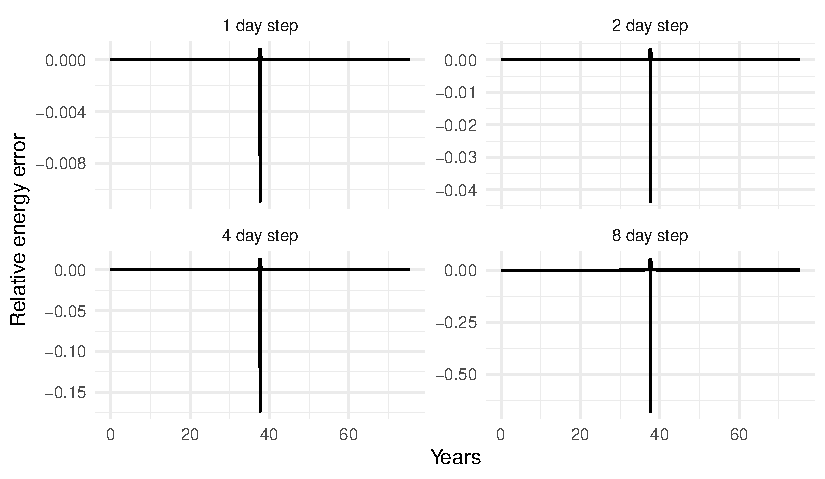
\includegraphics[width=1\linewidth,height=\textheight,keepaspectratio]{13-comets_files/figure-pdf/fig-halley-energy-1.pdf}

}

\caption{\label{fig-halley-energy}Relative energy error over one 75-year
orbit of Halley's Comet, started at aphelion, at four step sizes.
Nothing happens for 37 years; then the comet passes perihelion and the
integrator with the 8-day step hands it a large spurious kick.}

\end{figure}%

The shape is instructive. For the first 37 years the error is
essentially zero at every step size, because far from the Sun the
acceleration changes slowly and even an 8-day step is tiny compared with
the local timescale of years. Then, in the few weeks around perihelion,
each run makes all of its error at once. For the 1-day step the kick is
small and the comet comes out on nearly the right orbit. For the 8-day
step the kick is a substantial fraction of the comet's binding energy,
which means the comet leaves perihelion on a \emph{different orbit},
with a different period, and every subsequent apparition is at the wrong
time.

The error is \(O(\Delta t^2)\) in the usual way, as the ratios between
panels show, but that is cold comfort when the only way to shrink it is
to spend 27,000 steps on an orbit that needs a thousand. Two of the
three possible responses are bad.

\textbf{Softening is not the answer.} It would cap the force near the
Sun, which is exactly the force that is correct. Halley does not hit the
Sun. Softening would change the orbit to a wrong one at every
perihelion, smoothly and forever.

\textbf{A uniform small step works but wastes effort.} A 6-hour step is
safely inside the perihelion timescale and costs 110,000 steps per
orbit. For one comet that is fine, a minute or two of computing. For a
thousand comets, or a comet with a period of a thousand years, it is
not.

\section{Segmented runs}\label{segmented-runs}

The right response is to take small steps near perihelion and large
steps elsewhere. \texttt{simulate\_system()} integrates with one fixed
step, but nothing stops you from running it several times, because the
last row of a simulation tibble is a complete state.
\texttt{continue\_simulation()} does the bookkeeping: it rebuilds the
system from the final time step (\texttt{system\_from\_simulation()}
does that part on its own, if you want to edit the system between
segments), runs it onward with whatever step you give it, and appends
the new rows with \texttt{time} continuing from where the old run ended.
The gravitational constant, integrator, and softening carry over from
the previous segment unless you say otherwise.

Each segment is an ordinary Verlet run with all of Chapter 5's
guarantees; only at the switches is there any disturbance, and it is a
single step's worth.

When to switch? Say we want the small step inside 5 AU. Kepler's
equation, run in reverse, gives the time from perihelion to any true
anomaly, and the true anomaly at \(r = 5\) AU follows from the orbit
equation, \(\cos\nu = (p/r - 1)/e\) (the inverse-direction helper
\texttt{time\_since\_periapsis()} is in \texttt{R/helpers.R}):

\begin{Shaded}
\begin{Highlighting}[]
\NormalTok{p        }\OtherTok{\textless{}{-}}\NormalTok{ halley}\SpecialCharTok{$}\NormalTok{a }\SpecialCharTok{*}\NormalTok{ (}\DecValTok{1} \SpecialCharTok{{-}}\NormalTok{ halley}\SpecialCharTok{$}\NormalTok{e}\SpecialCharTok{\^{}}\DecValTok{2}\NormalTok{)}
\NormalTok{nu\_5AU   }\OtherTok{\textless{}{-}} \FunctionTok{acos}\NormalTok{((p }\SpecialCharTok{/}\NormalTok{ (}\DecValTok{5} \SpecialCharTok{*}\NormalTok{ AU) }\SpecialCharTok{{-}} \DecValTok{1}\NormalTok{) }\SpecialCharTok{/}\NormalTok{ halley}\SpecialCharTok{$}\NormalTok{e) }\SpecialCharTok{*} \DecValTok{180} \SpecialCharTok{/}\NormalTok{ pi}
\NormalTok{t\_inside }\OtherTok{\textless{}{-}} \FunctionTok{time\_since\_periapsis}\NormalTok{(nu\_5AU, halley}\SpecialCharTok{$}\NormalTok{a, halley}\SpecialCharTok{$}\NormalTok{e, mu\_sun)}

\FunctionTok{c}\NormalTok{(}\AttributeTok{nu\_at\_5AU\_deg =}\NormalTok{ nu\_5AU, }\AttributeTok{years\_inside\_5AU\_each\_way =}\NormalTok{ t\_inside }\SpecialCharTok{/}\NormalTok{ seconds\_per\_year)}
\CommentTok{\#\textgreater{}             nu\_at\_5AU\_deg years\_inside\_5AU\_each\_way }
\CommentTok{\#\textgreater{}                 142.71047                   1.02473}
\end{Highlighting}
\end{Shaded}

Halley spends about a year on each side of perihelion inside 5 AU, and
73 years outside. Three segments, then: coarse from aphelion to the 5 AU
crossing, fine through perihelion, coarse back out:

\begin{Shaded}
\begin{Highlighting}[]
\NormalTok{coarse }\OtherTok{\textless{}{-}}\NormalTok{ seconds\_per\_day }\SpecialCharTok{*} \DecValTok{8}
\NormalTok{fine   }\OtherTok{\textless{}{-}}\NormalTok{ seconds\_per\_hour }\SpecialCharTok{*} \DecValTok{6}
\NormalTok{t\_out  }\OtherTok{\textless{}{-}}\NormalTok{ T\_halley }\SpecialCharTok{/} \DecValTok{2} \SpecialCharTok{{-}}\NormalTok{ t\_inside           }\CommentTok{\# aphelion to the inbound crossing}

\NormalTok{segmented }\OtherTok{\textless{}{-}}\NormalTok{ halley\_system }\SpecialCharTok{|\textgreater{}}
  \FunctionTok{simulate\_system}\NormalTok{(}\AttributeTok{time\_step =}\NormalTok{ coarse, }\AttributeTok{duration =}\NormalTok{ t\_out) }\SpecialCharTok{|\textgreater{}}
  \FunctionTok{continue\_simulation}\NormalTok{(}\AttributeTok{time\_step =}\NormalTok{ fine,   }\AttributeTok{duration =} \DecValTok{2} \SpecialCharTok{*}\NormalTok{ t\_inside) }\SpecialCharTok{|\textgreater{}}
  \FunctionTok{continue\_simulation}\NormalTok{(}\AttributeTok{time\_step =}\NormalTok{ coarse, }\AttributeTok{duration =}\NormalTok{ t\_out)}

\FunctionTok{n\_distinct}\NormalTok{(segmented}\SpecialCharTok{$}\NormalTok{time)}
\CommentTok{\#\textgreater{} [1] 6339}
\end{Highlighting}
\end{Shaded}

A few thousand steps instead of 110,000, and the energy:

\begin{Shaded}
\begin{Highlighting}[]
\FunctionTok{bind\_rows}\NormalTok{(}
  \FunctionTok{conserved\_quantities}\NormalTok{(segmented) }\SpecialCharTok{|\textgreater{}} \FunctionTok{mutate}\NormalTok{(}\AttributeTok{run =} \StringTok{"Segmented: 8 d / 6 h / 8 d"}\NormalTok{),}
\NormalTok{  halley\_runs }\SpecialCharTok{|\textgreater{}} \FunctionTok{filter}\NormalTok{(step\_days }\SpecialCharTok{==} \DecValTok{8}\NormalTok{) }\SpecialCharTok{|\textgreater{}} \FunctionTok{mutate}\NormalTok{(}\AttributeTok{run =} \StringTok{"Uniform 8 d"}\NormalTok{)}
\NormalTok{) }\SpecialCharTok{|\textgreater{}}
  \FunctionTok{ggplot}\NormalTok{(}\FunctionTok{aes}\NormalTok{(time }\SpecialCharTok{/}\NormalTok{ seconds\_per\_year, energy\_error, }\AttributeTok{color =}\NormalTok{ run)) }\SpecialCharTok{+}
  \FunctionTok{geom\_line}\NormalTok{() }\SpecialCharTok{+}
  \FunctionTok{labs}\NormalTok{(}\AttributeTok{x =} \StringTok{"Years"}\NormalTok{, }\AttributeTok{y =} \StringTok{"Relative energy error"}\NormalTok{, }\AttributeTok{color =} \ConstantTok{NULL}\NormalTok{)}
\end{Highlighting}
\end{Shaded}

\begin{figure}[tbp]

\centering{

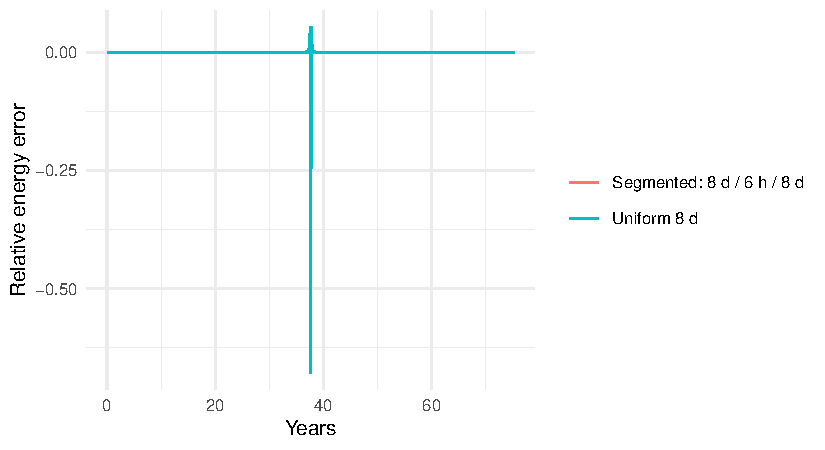
\includegraphics[width=1\linewidth,height=\textheight,keepaspectratio]{13-comets_files/figure-pdf/fig-segmented-1.pdf}

}

\caption{\label{fig-segmented}Energy error for the segmented run (8-day
steps outside 5 AU, 6-hour steps inside) compared with a uniform 8-day
run. The segmented run resolves the perihelion passage at a small
fraction of the cost of a uniform fine step.}

\end{figure}%

\begin{Shaded}
\begin{Highlighting}[]
\FunctionTok{c}\NormalTok{(}\AttributeTok{segmented =} \FunctionTok{max}\NormalTok{(}\FunctionTok{abs}\NormalTok{(}\FunctionTok{conserved\_quantities}\NormalTok{(segmented)}\SpecialCharTok{$}\NormalTok{energy\_error)),}
  \AttributeTok{uniform\_8\_day =} \FunctionTok{max}\NormalTok{(}\FunctionTok{abs}\NormalTok{(}\FunctionTok{filter}\NormalTok{(halley\_runs, step\_days }\SpecialCharTok{==} \DecValTok{8}\NormalTok{)}\SpecialCharTok{$}\NormalTok{energy\_error)),}
  \AttributeTok{uniform\_1\_day =} \FunctionTok{max}\NormalTok{(}\FunctionTok{abs}\NormalTok{(}\FunctionTok{filter}\NormalTok{(halley\_runs, step\_days }\SpecialCharTok{==} \DecValTok{1}\NormalTok{)}\SpecialCharTok{$}\NormalTok{energy\_error)))}
\CommentTok{\#\textgreater{}     segmented uniform\_8\_day uniform\_1\_day }
\CommentTok{\#\textgreater{}  0.0003968142  0.6776209618  0.0109308137}
\end{Highlighting}
\end{Shaded}

The segmented run beats the uniform daily run on accuracy at a fraction
of its cost. The idea generalizes: for a comet with many perihelion
passages, loop over them; for a system with one body that needs fine
steps and many that do not, you still pay for the fine steps on every
body (the package integrates them all together), which is the limitation
that true adaptive-step codes remove. Chapter 16 says why they are hard
to do without losing Verlet's symplectic guarantee.

\begin{tcolorbox}[enhanced jigsaw, arc=.35mm, bottomrule=.15mm, bottomtitle=1mm, breakable, colback=white, colbacktitle=quarto-callout-note-color!10!white, colframe=quarto-callout-note-color-frame, coltitle=black, left=2mm, leftrule=.75mm, opacityback=0, opacitybacktitle=0.6, rightrule=.15mm, title={Where it comes from}, titlerule=0mm, toprule=.15mm, toptitle=1mm]

Halley's Comet is the reason we know comets are periodic at all. Edmond
Halley, using Newton's new method, computed orbits for two dozen
historical comets and noticed that the ones of 1531, 1607, and 1682 had
nearly the same elements. He predicted a return in 1758, sixteen years
after his own death, and when it came the question of whether comets
obeyed gravity was settled. Alexis Clairaut refined the prediction to
within a month by computing the perturbations of Jupiter and Saturn, by
hand, over the preceding orbit, which was the first serious numerical
integration in celestial mechanics and took him and two assistants most
of a year.

\end{tcolorbox}

\section{Hyperbolic visitors}\label{hyperbolic-visitors}

In 2017 an object was found on an orbit with \(e = 1.2\). It was not
bound to the Sun at all; it had come from interstellar space and was on
its way back out. 'Oumuamua passed perihelion at 0.255 AU and was gone
within months.

The same six elements describe a hyperbola, with one twist: its
semi-major axis is \emph{negative}. The periapsis distance \(a(1-e)\)
stays positive, since both factors flip sign, and with \(a < 0\) and
\(e > 1\) the semi-latus rectum \(p = a(1-e^2)\) is positive,
\(h = \sqrt{\mu p}\) is real, and Equation~\ref{eq-pf-position} and
Equation~\ref{eq-pf-velocity} work unchanged.
\texttt{add\_body\_keplerian()} accepts \(e > 1\) when \texttt{a} is
negative, provided the starting true anomaly is within the asymptotes,
\(|\nu| < \arccos(-1/e)\) (it refuses \(e = 1\) exactly, where \(a\)
would be infinite):

\begin{Shaded}
\begin{Highlighting}[]
\NormalTok{e\_ou }\OtherTok{\textless{}{-}} \FloatTok{1.1995}
\NormalTok{q\_ou }\OtherTok{\textless{}{-}} \FloatTok{0.2553} \SpecialCharTok{*}\NormalTok{ AU}
\NormalTok{a\_ou }\OtherTok{\textless{}{-}} \SpecialCharTok{{-}}\NormalTok{q\_ou }\SpecialCharTok{/}\NormalTok{ (e\_ou }\SpecialCharTok{{-}} \DecValTok{1}\NormalTok{)                   }\CommentTok{\# negative for a hyperbola}

\FunctionTok{c}\NormalTok{(}\AttributeTok{asymptote\_deg =} \FunctionTok{acos}\NormalTok{(}\SpecialCharTok{{-}}\DecValTok{1} \SpecialCharTok{/}\NormalTok{ e\_ou) }\SpecialCharTok{*} \DecValTok{180} \SpecialCharTok{/}\NormalTok{ pi,}
  \AttributeTok{deflection\_deg =} \DecValTok{2} \SpecialCharTok{*} \FunctionTok{asin}\NormalTok{(}\DecValTok{1} \SpecialCharTok{/}\NormalTok{ e\_ou) }\SpecialCharTok{*} \DecValTok{180} \SpecialCharTok{/}\NormalTok{ pi)}
\CommentTok{\#\textgreater{}  asymptote\_deg deflection\_deg }
\CommentTok{\#\textgreater{}       146.4787       112.9574}

\NormalTok{oumuamua }\OtherTok{\textless{}{-}} \FunctionTok{create\_system}\NormalTok{() }\SpecialCharTok{|\textgreater{}}
  \FunctionTok{add\_sun}\NormalTok{() }\SpecialCharTok{|\textgreater{}}
  \FunctionTok{add\_body\_keplerian}\NormalTok{(}\StringTok{"Oumuamua"}\NormalTok{, }\AttributeTok{mass =} \FloatTok{1e10}\NormalTok{, }\AttributeTok{parent =} \StringTok{"Sun"}\NormalTok{,}
                     \AttributeTok{a =}\NormalTok{ a\_ou, }\AttributeTok{e =}\NormalTok{ e\_ou, }\AttributeTok{i =} \FloatTok{122.7}\NormalTok{, }\AttributeTok{lan =} \FloatTok{24.6}\NormalTok{,}
                     \AttributeTok{arg\_pe =} \FloatTok{241.8}\NormalTok{, }\AttributeTok{nu =} \SpecialCharTok{{-}}\DecValTok{140}\NormalTok{) }\SpecialCharTok{|\textgreater{}}
  \FunctionTok{simulate\_system}\NormalTok{(}\AttributeTok{time\_step =}\NormalTok{ seconds\_per\_hour, }\AttributeTok{duration =}\NormalTok{ seconds\_per\_year }\SpecialCharTok{*} \FloatTok{2.4}\NormalTok{)}
\end{Highlighting}
\end{Shaded}

\begin{Shaded}
\begin{Highlighting}[]
\NormalTok{rel }\OtherTok{\textless{}{-}} \FunctionTok{relative\_state}\NormalTok{(oumuamua, }\StringTok{"Oumuamua"}\NormalTok{, }\StringTok{"Sun"}\NormalTok{) }\SpecialCharTok{|\textgreater{}}
  \FunctionTok{mutate}\NormalTok{(}\AttributeTok{r =} \FunctionTok{sqrt}\NormalTok{(rx}\SpecialCharTok{\^{}}\DecValTok{2} \SpecialCharTok{+}\NormalTok{ ry}\SpecialCharTok{\^{}}\DecValTok{2} \SpecialCharTok{+}\NormalTok{ rz}\SpecialCharTok{\^{}}\DecValTok{2}\NormalTok{), }\AttributeTok{v =} \FunctionTok{sqrt}\NormalTok{(ux}\SpecialCharTok{\^{}}\DecValTok{2} \SpecialCharTok{+}\NormalTok{ uy}\SpecialCharTok{\^{}}\DecValTok{2} \SpecialCharTok{+}\NormalTok{ uz}\SpecialCharTok{\^{}}\DecValTok{2}\NormalTok{),}
         \AttributeTok{energy =}\NormalTok{ v}\SpecialCharTok{\^{}}\DecValTok{2} \SpecialCharTok{/} \DecValTok{2} \SpecialCharTok{{-}}\NormalTok{ mu }\SpecialCharTok{/}\NormalTok{ r)}

\FunctionTok{c}\NormalTok{(}\AttributeTok{r\_start\_AU =} \FunctionTok{first}\NormalTok{(rel}\SpecialCharTok{$}\NormalTok{r) }\SpecialCharTok{/}\NormalTok{ AU, }\AttributeTok{r\_end\_AU =} \FunctionTok{last}\NormalTok{(rel}\SpecialCharTok{$}\NormalTok{r) }\SpecialCharTok{/}\NormalTok{ AU,}
  \AttributeTok{v\_max\_km\_s =} \FunctionTok{max}\NormalTok{(rel}\SpecialCharTok{$}\NormalTok{v) }\SpecialCharTok{/} \FloatTok{1e3}\NormalTok{,}
  \AttributeTok{v\_perihelion\_predicted =} \FunctionTok{sqrt}\NormalTok{(mu\_sun }\SpecialCharTok{*}\NormalTok{ (}\DecValTok{1} \SpecialCharTok{+}\NormalTok{ e\_ou) }\SpecialCharTok{/}\NormalTok{ q\_ou) }\SpecialCharTok{/} \FloatTok{1e3}\NormalTok{,}
  \AttributeTok{energy\_min =} \FunctionTok{min}\NormalTok{(rel}\SpecialCharTok{$}\NormalTok{energy), }\AttributeTok{energy\_max =} \FunctionTok{max}\NormalTok{(rel}\SpecialCharTok{$}\NormalTok{energy))}
\CommentTok{\#\textgreater{}             r\_start\_AU               r\_end\_AU             v\_max\_km\_s }
\CommentTok{\#\textgreater{}           6.921416e+00           1.061724e+01           8.743576e+01 }
\CommentTok{\#\textgreater{} v\_perihelion\_predicted             energy\_min             energy\_max }
\CommentTok{\#\textgreater{}           8.743615e+01           3.466985e+08           3.467151e+08}
\end{Highlighting}
\end{Shaded}

The specific energy is positive and constant, the maximum speed is the
vis-viva prediction at perihelion (\(v_p^2 = \mu(1+e)/q\), from
\(a \to\) negative in Equation~\ref{eq-vis-viva}), and the eccentricity
at the end is the eccentricity at the start:

\begin{Shaded}
\begin{Highlighting}[]
\FunctionTok{range}\NormalTok{(}\FunctionTok{get\_orbital\_elements}\NormalTok{(oumuamua, }\StringTok{"Oumuamua"}\NormalTok{, }\StringTok{"Sun"}\NormalTok{)}\SpecialCharTok{$}\NormalTok{e)}
\CommentTok{\#\textgreater{} [1] 1.199492 1.199501}
\end{Highlighting}
\end{Shaded}

The object came in at 26 km/s relative to the Sun and left at 26 km/s,
deflected through the angle \(2\arcsin(1/e)\) of about 113 degrees. (The
real 'Oumuamua showed a small extra acceleration away from the Sun that
gravity alone cannot produce, most likely outgassing, which is a
non-gravitational force of the kind Chapter 16 discusses.)

\section{Sungrazers}\label{sungrazers}

The Kreutz family of comets, hundreds of which have been seen by solar
observatories, have perihelia around 0.005 AU, about one solar radius.
Vis-viva at that distance gives

\begin{Shaded}
\begin{Highlighting}[]
\NormalTok{R\_sun }\OtherTok{\textless{}{-}} \FloatTok{6.957e8}
\FunctionTok{sqrt}\NormalTok{(}\DecValTok{2} \SpecialCharTok{*}\NormalTok{ mu\_sun }\SpecialCharTok{/}\NormalTok{ R\_sun) }\SpecialCharTok{/} \FloatTok{1e3}
\CommentTok{\#\textgreater{} [1] 617.7664}
\end{Highlighting}
\end{Shaded}

kilometers per second, over six hundred, which is the escape speed from
the Sun's surface, since these comets arrive on nearly parabolic orbits.
Most of them do not survive. The simulation would carry them through
without comment: the Sun is a point, the comet is a point, and two
points can pass within a solar radius, or within a meter, and the
integrator will either resolve it (with a step of minutes) or produce
the spurious kick of Chapter 6. The package roadmap's \texttt{radius}
argument and collision handling are the fix; until then, a Kreutz comet
is a case where the physics the package implements and the physics that
happens part company, and the simulation's answer should be read as ``it
would have hit.''

\begin{tcolorbox}[enhanced jigsaw, arc=.35mm, bottomrule=.15mm, bottomtitle=1mm, breakable, colback=white, colbacktitle=quarto-callout-tip-color!10!white, colframe=quarto-callout-tip-color-frame, coltitle=black, left=2mm, leftrule=.75mm, opacityback=0, opacitybacktitle=0.6, rightrule=.15mm, title={Key results}, titlerule=0mm, toprule=.15mm, toptitle=1mm]

\begin{itemize}
\tightlist
\item
  A fixed step must resolve the perihelion timescale \(q/v_p\), where
  \(v_p^2 = \mu(1+e)/q\); for Halley that is weeks, for a sungrazer
  minutes.
\item
  A too-large step makes its whole error in one perihelion kick and
  leaves the comet on a different orbit.
\item
  \texttt{continue\_simulation()} lets you change the step between
  segments; Kepler's equation tells you when to switch. Softening is
  never the fix.
\item
  Hyperbolic orbits (\(e > 1\), \(a < 0\)) work in
  \texttt{add\_body\_keplerian()}; the visitor leaves with the speed it
  came with, deflected by \(2\arcsin(1/e)\).
\end{itemize}

\end{tcolorbox}

\chapter{Figures for Papers and Talks}\label{sec-figures}

The plotting functions in orbitr are built to get you a picture in one
line so that you can get back to the physics. That is the right design
for exploring and the wrong one for publishing, where the picture needs
the units, labels, colors, and size that your journal or your slides
demand. The good news is that there is no gap between the two:
\texttt{plot\_orbits()} returns a ggplot you can keep modifying, and
everything else is a tibble you can plot however you like. This chapter
is the short, practical one. It collects the plotting patterns the rest
of the book has been using, adds the ones a paper or a talk needs, and
says where the interactive and animated output fits.

\section{\texorpdfstring{\texttt{plot\_orbits()} is a
ggplot}{plot\_orbits() is a ggplot}}\label{plot_orbits-is-a-ggplot}

Anything you can add to a ggplot you can add to the output of
\texttt{plot\_orbits()}. The most common fixes are a marker for the
central body, which is otherwise invisible because it barely moves; axis
labels in sensible units; and a theme:

\begin{Shaded}
\begin{Highlighting}[]
\NormalTok{AU }\OtherTok{\textless{}{-}}\NormalTok{ distance\_earth\_sun}

\NormalTok{inner }\OtherTok{\textless{}{-}} \FunctionTok{create\_system}\NormalTok{() }\SpecialCharTok{|\textgreater{}}
  \FunctionTok{add\_sun}\NormalTok{() }\SpecialCharTok{|\textgreater{}}
  \FunctionTok{add\_planet}\NormalTok{(}\StringTok{"Mercury"}\NormalTok{, }\AttributeTok{parent =} \StringTok{"Sun"}\NormalTok{) }\SpecialCharTok{|\textgreater{}}
  \FunctionTok{add\_planet}\NormalTok{(}\StringTok{"Venus"}\NormalTok{,   }\AttributeTok{parent =} \StringTok{"Sun"}\NormalTok{) }\SpecialCharTok{|\textgreater{}}
  \FunctionTok{add\_planet}\NormalTok{(}\StringTok{"Earth"}\NormalTok{,   }\AttributeTok{parent =} \StringTok{"Sun"}\NormalTok{) }\SpecialCharTok{|\textgreater{}}
  \FunctionTok{add\_planet}\NormalTok{(}\StringTok{"Mars"}\NormalTok{,    }\AttributeTok{parent =} \StringTok{"Sun"}\NormalTok{) }\SpecialCharTok{|\textgreater{}}
  \FunctionTok{simulate\_system}\NormalTok{(}\AttributeTok{time\_step =}\NormalTok{ seconds\_per\_day, }\AttributeTok{duration =}\NormalTok{ seconds\_per\_year)}

\FunctionTok{plot\_orbits}\NormalTok{(inner, }\AttributeTok{three\_d =} \ConstantTok{FALSE}\NormalTok{) }\SpecialCharTok{+}
  \FunctionTok{annotate}\NormalTok{(}\StringTok{"point"}\NormalTok{, }\AttributeTok{x =} \DecValTok{0}\NormalTok{, }\AttributeTok{y =} \DecValTok{0}\NormalTok{, }\AttributeTok{size =} \DecValTok{3}\NormalTok{) }\SpecialCharTok{+}
  \FunctionTok{scale\_x\_continuous}\NormalTok{(}\AttributeTok{labels =} \ControlFlowTok{function}\NormalTok{(m) m }\SpecialCharTok{/}\NormalTok{ AU) }\SpecialCharTok{+}
  \FunctionTok{scale\_y\_continuous}\NormalTok{(}\AttributeTok{labels =} \ControlFlowTok{function}\NormalTok{(m) m }\SpecialCharTok{/}\NormalTok{ AU) }\SpecialCharTok{+}
  \FunctionTok{labs}\NormalTok{(}\AttributeTok{x =} \StringTok{"x (AU)"}\NormalTok{, }\AttributeTok{y =} \StringTok{"y (AU)"}\NormalTok{, }\AttributeTok{color =} \ConstantTok{NULL}\NormalTok{)}
\end{Highlighting}
\end{Shaded}

\begin{figure}[tbp]

\centering{

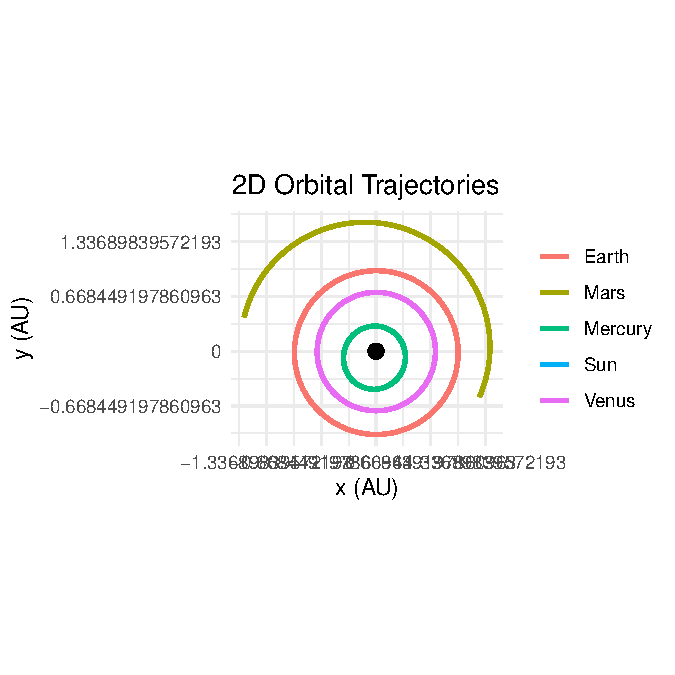
\includegraphics[width=0.65\linewidth,height=\textheight,keepaspectratio]{14-figures-for-papers-and-talks_files/figure-pdf/fig-layered-1.pdf}

}

\caption{\label{fig-layered}The default plot with three additions: a
marker for the Sun, axis labels, and a scale in AU.}

\end{figure}%

The scale functions relabel the axes without touching the data, which
keeps \texttt{coord\_equal()} honest. If you would rather convert the
data, do it before plotting, as the next section does.

\section{Your own plots from the
tibble}\label{your-own-plots-from-the-tibble}

The built-in plot draws one path per body. Everything else is a
\texttt{mutate()} and a \texttt{ggplot()}. Four patterns cover most
needs.

\textbf{Color by time}, to show direction and speed along a path:

\begin{Shaded}
\begin{Highlighting}[]
\FunctionTok{create\_system}\NormalTok{() }\SpecialCharTok{|\textgreater{}}
  \FunctionTok{add\_sun}\NormalTok{() }\SpecialCharTok{|\textgreater{}}
  \FunctionTok{add\_planet}\NormalTok{(}\StringTok{"Earth"}\NormalTok{, }\AttributeTok{parent =} \StringTok{"Sun"}\NormalTok{) }\SpecialCharTok{|\textgreater{}}
  \FunctionTok{add\_planet}\NormalTok{(}\StringTok{"Mars"}\NormalTok{,  }\AttributeTok{parent =} \StringTok{"Sun"}\NormalTok{, }\AttributeTok{nu =} \DecValTok{60}\NormalTok{) }\SpecialCharTok{|\textgreater{}}
  \FunctionTok{simulate\_system}\NormalTok{(}\AttributeTok{time\_step =}\NormalTok{ seconds\_per\_day, }\AttributeTok{duration =}\NormalTok{ seconds\_per\_year }\SpecialCharTok{*} \FloatTok{2.2}\NormalTok{) }\SpecialCharTok{|\textgreater{}}
  \FunctionTok{shift\_reference\_frame}\NormalTok{(}\StringTok{"Earth"}\NormalTok{, }\AttributeTok{keep\_center =} \ConstantTok{FALSE}\NormalTok{) }\SpecialCharTok{|\textgreater{}}
  \FunctionTok{filter}\NormalTok{(id }\SpecialCharTok{==} \StringTok{"Mars"}\NormalTok{) }\SpecialCharTok{|\textgreater{}}
  \FunctionTok{ggplot}\NormalTok{(}\FunctionTok{aes}\NormalTok{(x }\SpecialCharTok{/}\NormalTok{ AU, y }\SpecialCharTok{/}\NormalTok{ AU, }\AttributeTok{color =}\NormalTok{ time }\SpecialCharTok{/}\NormalTok{ seconds\_per\_year)) }\SpecialCharTok{+}
  \FunctionTok{geom\_path}\NormalTok{(}\AttributeTok{linewidth =} \FloatTok{0.9}\NormalTok{) }\SpecialCharTok{+}
  \FunctionTok{scale\_color\_viridis\_c}\NormalTok{() }\SpecialCharTok{+}
  \FunctionTok{coord\_equal}\NormalTok{() }\SpecialCharTok{+}
  \FunctionTok{labs}\NormalTok{(}\AttributeTok{x =} \StringTok{"x (AU)"}\NormalTok{, }\AttributeTok{y =} \StringTok{"y (AU)"}\NormalTok{, }\AttributeTok{color =} \StringTok{"Years"}\NormalTok{)}
\end{Highlighting}
\end{Shaded}

\begin{figure}[tbp]

\centering{

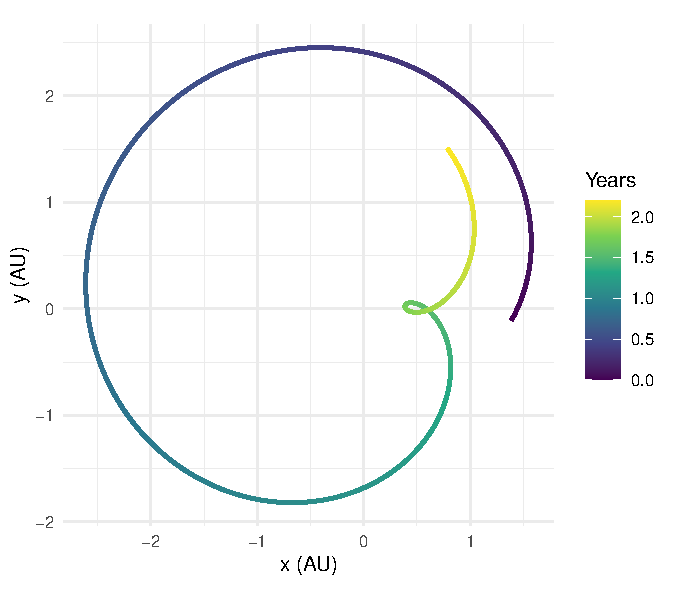
\includegraphics[width=0.65\linewidth,height=\textheight,keepaspectratio]{14-figures-for-papers-and-talks_files/figure-pdf/fig-color-time-1.pdf}

}

\caption{\label{fig-color-time}Mars seen from Earth over two years,
colored by time. The color gradient makes the direction of motion and
the retrograde loop readable without an animation.}

\end{figure}%

\textbf{Time series} of any derived quantity: distance, speed, energy,
an orbital element. The pattern is always \texttt{mutate()} the
quantity, then \texttt{aes(time,\ quantity)}:

\begin{Shaded}
\begin{Highlighting}[]
\FunctionTok{create\_system}\NormalTok{() }\SpecialCharTok{|\textgreater{}}
  \FunctionTok{add\_sun}\NormalTok{() }\SpecialCharTok{|\textgreater{}}
  \FunctionTok{add\_planet}\NormalTok{(}\StringTok{"Mercury"}\NormalTok{, }\AttributeTok{parent =} \StringTok{"Sun"}\NormalTok{) }\SpecialCharTok{|\textgreater{}}
  \FunctionTok{simulate\_system}\NormalTok{(}\AttributeTok{time\_step =}\NormalTok{ seconds\_per\_hour }\SpecialCharTok{*} \DecValTok{6}\NormalTok{, }\AttributeTok{duration =}\NormalTok{ seconds\_per\_day }\SpecialCharTok{*} \DecValTok{88}\NormalTok{) }\SpecialCharTok{|\textgreater{}}
  \FunctionTok{shift\_reference\_frame}\NormalTok{(}\StringTok{"Sun"}\NormalTok{, }\AttributeTok{keep\_center =} \ConstantTok{FALSE}\NormalTok{) }\SpecialCharTok{|\textgreater{}}
  \FunctionTok{transmute}\NormalTok{(}\AttributeTok{day =}\NormalTok{ time }\SpecialCharTok{/}\NormalTok{ seconds\_per\_day,}
            \StringTok{\textasciigrave{}}\AttributeTok{Distance (AU)}\StringTok{\textasciigrave{}} \OtherTok{=} \FunctionTok{sqrt}\NormalTok{(x}\SpecialCharTok{\^{}}\DecValTok{2} \SpecialCharTok{+}\NormalTok{ y}\SpecialCharTok{\^{}}\DecValTok{2} \SpecialCharTok{+}\NormalTok{ z}\SpecialCharTok{\^{}}\DecValTok{2}\NormalTok{) }\SpecialCharTok{/}\NormalTok{ AU,}
            \StringTok{\textasciigrave{}}\AttributeTok{Speed (km/s)}\StringTok{\textasciigrave{}}  \OtherTok{=} \FunctionTok{sqrt}\NormalTok{(vx}\SpecialCharTok{\^{}}\DecValTok{2} \SpecialCharTok{+}\NormalTok{ vy}\SpecialCharTok{\^{}}\DecValTok{2} \SpecialCharTok{+}\NormalTok{ vz}\SpecialCharTok{\^{}}\DecValTok{2}\NormalTok{) }\SpecialCharTok{/} \FloatTok{1e3}\NormalTok{) }\SpecialCharTok{|\textgreater{}}
\NormalTok{  tidyr}\SpecialCharTok{::}\FunctionTok{pivot\_longer}\NormalTok{(}\SpecialCharTok{{-}}\NormalTok{day) }\SpecialCharTok{|\textgreater{}}
  \FunctionTok{ggplot}\NormalTok{(}\FunctionTok{aes}\NormalTok{(day, value)) }\SpecialCharTok{+}
  \FunctionTok{geom\_line}\NormalTok{() }\SpecialCharTok{+}
  \FunctionTok{facet\_wrap}\NormalTok{(}\SpecialCharTok{\textasciitilde{}}\NormalTok{ name, }\AttributeTok{scales =} \StringTok{"free\_y"}\NormalTok{, }\AttributeTok{ncol =} \DecValTok{1}\NormalTok{) }\SpecialCharTok{+}
  \FunctionTok{labs}\NormalTok{(}\AttributeTok{x =} \StringTok{"Day"}\NormalTok{, }\AttributeTok{y =} \ConstantTok{NULL}\NormalTok{)}
\end{Highlighting}
\end{Shaded}

\begin{figure}[tbp]

\centering{

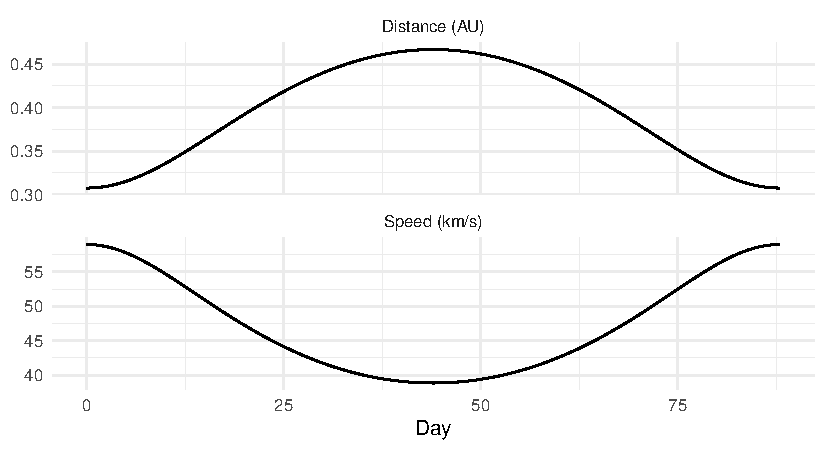
\includegraphics[width=1\linewidth,height=\textheight,keepaspectratio]{14-figures-for-papers-and-talks_files/figure-pdf/fig-time-series-1.pdf}

}

\caption{\label{fig-time-series}Mercury's heliocentric distance and
speed over one orbit, as time series. Two panels from one tibble via
pivot\_longer().}

\end{figure}%

\textbf{Small multiples} with \texttt{facet\_wrap()}, which is how most
of this book's comparisons were drawn: give each run a label column with
\texttt{mutate(run\ =\ "...")}, \texttt{bind\_rows()} them, and facet by
it. Chapter 5's integrator comparison and Chapter 6's encounter figure
are both this pattern.

\textbf{Snapshots in a grid.} \texttt{plot\_system()} draws one instant.
For a sequence of instants in a paper, where an animation is not an
option, overlay the full paths in grey and facet the positions by time:

\begin{Shaded}
\begin{Highlighting}[]
\NormalTok{days }\OtherTok{\textless{}{-}} \FunctionTok{c}\NormalTok{(}\DecValTok{0}\NormalTok{, }\DecValTok{90}\NormalTok{, }\DecValTok{180}\NormalTok{, }\DecValTok{270}\NormalTok{)}

\NormalTok{snapshots }\OtherTok{\textless{}{-}} \FunctionTok{bind\_rows}\NormalTok{(}\FunctionTok{lapply}\NormalTok{(days, }\ControlFlowTok{function}\NormalTok{(d) \{}
\NormalTok{  inner }\SpecialCharTok{|\textgreater{}}
    \FunctionTok{filter}\NormalTok{(}\FunctionTok{abs}\NormalTok{(time }\SpecialCharTok{{-}}\NormalTok{ d }\SpecialCharTok{*}\NormalTok{ seconds\_per\_day) }\SpecialCharTok{\textless{}}\NormalTok{ seconds\_per\_day }\SpecialCharTok{/} \DecValTok{2}\NormalTok{) }\SpecialCharTok{|\textgreater{}}
    \FunctionTok{mutate}\NormalTok{(}\AttributeTok{day =} \FunctionTok{paste}\NormalTok{(}\StringTok{"Day"}\NormalTok{, d))}
\NormalTok{\}))}

\FunctionTok{ggplot}\NormalTok{() }\SpecialCharTok{+}
  \FunctionTok{geom\_path}\NormalTok{(}\AttributeTok{data =}\NormalTok{ inner, }\FunctionTok{aes}\NormalTok{(x }\SpecialCharTok{/}\NormalTok{ AU, y }\SpecialCharTok{/}\NormalTok{ AU, }\AttributeTok{group =}\NormalTok{ id), }\AttributeTok{color =} \StringTok{"grey80"}\NormalTok{) }\SpecialCharTok{+}
  \FunctionTok{geom\_point}\NormalTok{(}\AttributeTok{data =}\NormalTok{ snapshots, }\FunctionTok{aes}\NormalTok{(x }\SpecialCharTok{/}\NormalTok{ AU, y }\SpecialCharTok{/}\NormalTok{ AU, }\AttributeTok{color =}\NormalTok{ id), }\AttributeTok{size =} \DecValTok{2}\NormalTok{) }\SpecialCharTok{+}
  \FunctionTok{annotate}\NormalTok{(}\StringTok{"point"}\NormalTok{, }\AttributeTok{x =} \DecValTok{0}\NormalTok{, }\AttributeTok{y =} \DecValTok{0}\NormalTok{, }\AttributeTok{size =} \DecValTok{2}\NormalTok{) }\SpecialCharTok{+}
  \FunctionTok{coord\_equal}\NormalTok{() }\SpecialCharTok{+}
  \FunctionTok{facet\_wrap}\NormalTok{(}\SpecialCharTok{\textasciitilde{}}\NormalTok{ day) }\SpecialCharTok{+}
  \FunctionTok{labs}\NormalTok{(}\AttributeTok{x =} \StringTok{"x (AU)"}\NormalTok{, }\AttributeTok{y =} \StringTok{"y (AU)"}\NormalTok{, }\AttributeTok{color =} \ConstantTok{NULL}\NormalTok{)}
\end{Highlighting}
\end{Shaded}

\begin{figure}[tbp]

\centering{

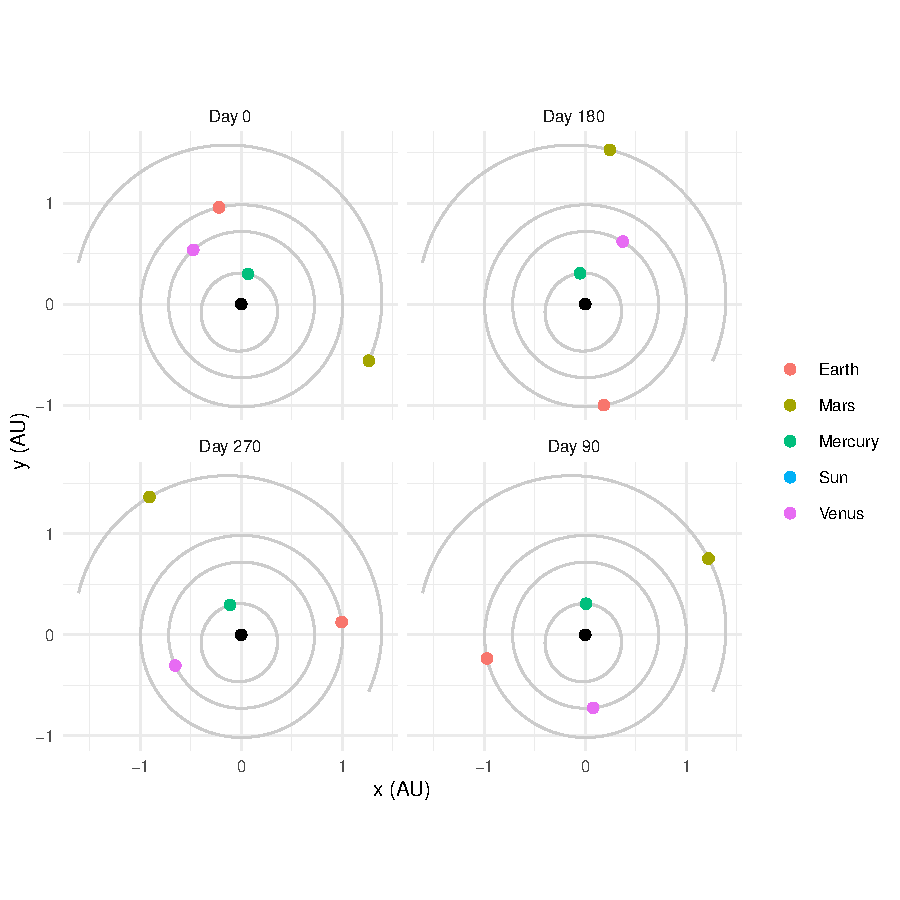
\includegraphics[width=0.85\linewidth,height=\textheight,keepaspectratio]{14-figures-for-papers-and-talks_files/figure-pdf/fig-snapshot-grid-1.pdf}

}

\caption{\label{fig-snapshot-grid}The inner solar system at four
instants, with the full year's paths behind. A static substitute for an
animation.}

\end{figure}%

\section{A figure for a paper}\label{a-figure-for-a-paper}

A journal figure has a few requirements that an exploratory plot does
not: a fixed physical size, a font size that will still be legible after
the figure is shrunk to a column, a color scheme that survives greyscale
printing and colorblind readers, and vector output. Here is a recipe:

\begin{Shaded}
\begin{Highlighting}[]
\NormalTok{star\_planet }\OtherTok{\textless{}{-}} \FunctionTok{create\_system}\NormalTok{() }\SpecialCharTok{|\textgreater{}}
  \FunctionTok{add\_body}\NormalTok{(}\StringTok{"Star"}\NormalTok{,   }\AttributeTok{mass =} \FloatTok{1e30}\NormalTok{) }\SpecialCharTok{|\textgreater{}}
  \FunctionTok{add\_body}\NormalTok{(}\StringTok{"Planet"}\NormalTok{, }\AttributeTok{mass =} \FloatTok{1e24}\NormalTok{, }\AttributeTok{x =} \FloatTok{1e11}\NormalTok{, }\AttributeTok{vy =} \DecValTok{30000}\NormalTok{)}

\NormalTok{comparison }\OtherTok{\textless{}{-}} \FunctionTok{bind\_rows}\NormalTok{(}\FunctionTok{lapply}\NormalTok{(}\FunctionTok{c}\NormalTok{(}\StringTok{"verlet"}\NormalTok{, }\StringTok{"euler"}\NormalTok{), }\ControlFlowTok{function}\NormalTok{(m) \{}
\NormalTok{  star\_planet }\SpecialCharTok{|\textgreater{}}
    \FunctionTok{simulate\_system}\NormalTok{(}\AttributeTok{time\_step =}\NormalTok{ seconds\_per\_hour }\SpecialCharTok{*} \DecValTok{6}\NormalTok{,}
                    \AttributeTok{duration =}\NormalTok{ seconds\_per\_year }\SpecialCharTok{*} \DecValTok{6}\NormalTok{, }\AttributeTok{method =}\NormalTok{ m) }\SpecialCharTok{|\textgreater{}}
    \FunctionTok{filter}\NormalTok{(id }\SpecialCharTok{==} \StringTok{"Planet"}\NormalTok{) }\SpecialCharTok{|\textgreater{}}
    \FunctionTok{mutate}\NormalTok{(}\AttributeTok{method =} \FunctionTok{c}\NormalTok{(}\AttributeTok{verlet =} \StringTok{"Velocity Verlet"}\NormalTok{, }\AttributeTok{euler =} \StringTok{"Euler"}\NormalTok{)[m])}
\NormalTok{\}))}

\NormalTok{paper\_figure }\OtherTok{\textless{}{-}}\NormalTok{ comparison }\SpecialCharTok{|\textgreater{}}
  \FunctionTok{ggplot}\NormalTok{(}\FunctionTok{aes}\NormalTok{(x }\SpecialCharTok{/}\NormalTok{ AU, y }\SpecialCharTok{/}\NormalTok{ AU, }\AttributeTok{color =}\NormalTok{ method, }\AttributeTok{linetype =}\NormalTok{ method)) }\SpecialCharTok{+}
  \FunctionTok{geom\_path}\NormalTok{(}\AttributeTok{linewidth =} \FloatTok{0.5}\NormalTok{) }\SpecialCharTok{+}
  \FunctionTok{annotate}\NormalTok{(}\StringTok{"point"}\NormalTok{, }\AttributeTok{x =} \DecValTok{0}\NormalTok{, }\AttributeTok{y =} \DecValTok{0}\NormalTok{, }\AttributeTok{size =} \FloatTok{2.5}\NormalTok{) }\SpecialCharTok{+}
  \FunctionTok{scale\_color\_brewer}\NormalTok{(}\AttributeTok{palette =} \StringTok{"Dark2"}\NormalTok{) }\SpecialCharTok{+}
  \FunctionTok{coord\_equal}\NormalTok{() }\SpecialCharTok{+}
  \FunctionTok{labs}\NormalTok{(}\AttributeTok{x =} \StringTok{"x (AU)"}\NormalTok{, }\AttributeTok{y =} \StringTok{"y (AU)"}\NormalTok{, }\AttributeTok{color =} \ConstantTok{NULL}\NormalTok{, }\AttributeTok{linetype =} \ConstantTok{NULL}\NormalTok{) }\SpecialCharTok{+}
  \FunctionTok{theme\_classic}\NormalTok{(}\AttributeTok{base\_size =} \DecValTok{9}\NormalTok{) }\SpecialCharTok{+}
  \FunctionTok{theme}\NormalTok{(}\AttributeTok{legend.position =} \StringTok{"bottom"}\NormalTok{)}

\NormalTok{paper\_figure}
\end{Highlighting}
\end{Shaded}

\begin{figure}[tbp]

\centering{

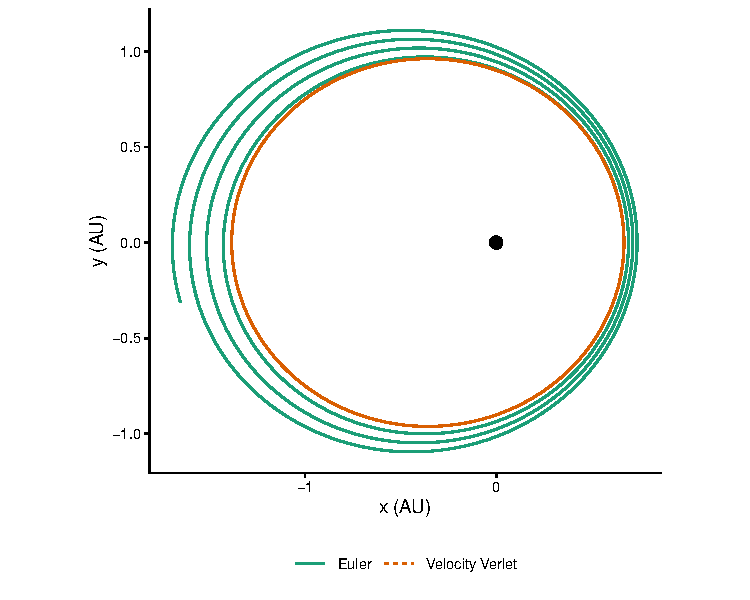
\includegraphics[width=0.7\linewidth,height=\textheight,keepaspectratio]{14-figures-for-papers-and-talks_files/figure-pdf/fig-paper-1.pdf}

}

\caption{\label{fig-paper}A publication-style version of Chapter 5's
integrator comparison: colorblind-safe palette, distinct line types so
the figure works in greyscale, a classic theme, and labels in the units
a reader expects.}

\end{figure}%

Save it at the size it will be printed, as a vector file:

\begin{Shaded}
\begin{Highlighting}[]
\FunctionTok{ggsave}\NormalTok{(}\StringTok{"integrators.pdf"}\NormalTok{, paper\_figure, }\AttributeTok{width =} \FloatTok{3.4}\NormalTok{, }\AttributeTok{height =} \FloatTok{3.0}\NormalTok{, }\AttributeTok{units =} \StringTok{"in"}\NormalTok{)}
\FunctionTok{ggsave}\NormalTok{(}\StringTok{"integrators.png"}\NormalTok{, paper\_figure, }\AttributeTok{width =} \FloatTok{3.4}\NormalTok{, }\AttributeTok{height =} \FloatTok{3.0}\NormalTok{, }\AttributeTok{units =} \StringTok{"in"}\NormalTok{,}
       \AttributeTok{dpi =} \DecValTok{600}\NormalTok{)}
\end{Highlighting}
\end{Shaded}

A single-column figure in most journals is about 3.4 inches wide; set
\texttt{base\_size} so that the text is 7 to 9 points at that size. The
PDF is what you submit; the PNG is for the slide.

Two things to watch. Orbit plots need \texttt{coord\_equal()}, or
circles become ellipses and the eye reads an eccentricity that is not
there. And when the data span orders of magnitude, as a comet's distance
does, a logarithmic axis (\texttt{scale\_y\_log10()}) is usually right,
as it was in Chapter 11.

\section{Interactive 3D for the
screen}\label{interactive-3d-for-the-screen}

Any system with motion out of the plane dispatches to plotly
automatically, and \texttt{plot\_orbits\_3d()} and
\texttt{plot\_system\_3d()} force it:

\begin{Shaded}
\begin{Highlighting}[]
\FunctionTok{load\_solar\_system}\NormalTok{() }\SpecialCharTok{|\textgreater{}}
  \FunctionTok{remove\_body}\NormalTok{(}\StringTok{"Moon"}\NormalTok{) }\SpecialCharTok{|\textgreater{}}
  \FunctionTok{simulate\_system}\NormalTok{(}\AttributeTok{time\_step =}\NormalTok{ seconds\_per\_day, }\AttributeTok{duration =}\NormalTok{ seconds\_per\_year }\SpecialCharTok{*} \DecValTok{30}\NormalTok{) }\SpecialCharTok{|\textgreater{}}
  \FunctionTok{plot\_orbits\_3d}\NormalTok{()}
\end{Highlighting}
\end{Shaded}

You can rotate, zoom, and hover for the time stamp. For a talk, the
widget can be saved as a self-contained HTML file and opened in any
browser:

\begin{Shaded}
\begin{Highlighting}[]
\NormalTok{p }\OtherTok{\textless{}{-}} \FunctionTok{plot\_orbits\_3d}\NormalTok{(sim)}
\NormalTok{htmlwidgets}\SpecialCharTok{::}\FunctionTok{saveWidget}\NormalTok{(p, }\StringTok{"solar{-}system{-}3d.html"}\NormalTok{, }\AttributeTok{selfcontained =} \ConstantTok{TRUE}\NormalTok{)}
\end{Highlighting}
\end{Shaded}

When you need more than the convenience function offers, build the
plotly figure from the tibble. The documentation's custom-visualization
article colors the Moon's path by speed with a \texttt{plot\_ly()} call;
the same idea works for any quantity you can \texttt{mutate()}. For a
static image of a 3D view, the usual route is a screenshot at the
orientation you want, or \texttt{plotly::save\_image()}, which needs the
\texttt{kaleido} Python package installed through \texttt{reticulate}.

\section{Animation}\label{animation}

\texttt{animate\_system()} samples the run into
\texttt{fps\ *\ duration} frames and renders a GIF with gganimate:

\begin{Shaded}
\begin{Highlighting}[]
\NormalTok{anim }\OtherTok{\textless{}{-}} \FunctionTok{animate\_system}\NormalTok{(inner, }\AttributeTok{fps =} \DecValTok{20}\NormalTok{, }\AttributeTok{duration =} \DecValTok{8}\NormalTok{, }\AttributeTok{trails =} \ConstantTok{TRUE}\NormalTok{)}
\NormalTok{anim}
\end{Highlighting}
\end{Shaded}

\begin{Shaded}
\begin{Highlighting}[]
\NormalTok{gganimate}\SpecialCharTok{::}\FunctionTok{anim\_save}\NormalTok{(}\StringTok{"inner{-}solar{-}system.gif"}\NormalTok{, anim)}
\end{Highlighting}
\end{Shaded}

Rendering takes tens of seconds, so get the static version right first,
and keep \texttt{fps\ *\ duration} modest: 160 frames is plenty for a
slide. A GIF loops forever and works in every slide program, which is
usually what you want. If you need an MP4, or control over the frame
labels, build the animation yourself from the tibble with gganimate,
which is a few lines:

\begin{Shaded}
\begin{Highlighting}[]
\FunctionTok{library}\NormalTok{(gganimate)}

\NormalTok{frames }\OtherTok{\textless{}{-}}\NormalTok{ inner }\SpecialCharTok{|\textgreater{}} \FunctionTok{filter}\NormalTok{(time }\SpecialCharTok{\%\%}\NormalTok{ (seconds\_per\_day }\SpecialCharTok{*} \DecValTok{5}\NormalTok{) }\SpecialCharTok{==} \DecValTok{0}\NormalTok{)   }\CommentTok{\# every 5th day}

\NormalTok{p }\OtherTok{\textless{}{-}} \FunctionTok{ggplot}\NormalTok{(frames, }\FunctionTok{aes}\NormalTok{(x }\SpecialCharTok{/}\NormalTok{ AU, y }\SpecialCharTok{/}\NormalTok{ AU, }\AttributeTok{color =}\NormalTok{ id)) }\SpecialCharTok{+}
  \FunctionTok{geom\_point}\NormalTok{(}\AttributeTok{size =} \DecValTok{3}\NormalTok{) }\SpecialCharTok{+}
  \FunctionTok{coord\_equal}\NormalTok{() }\SpecialCharTok{+}
  \FunctionTok{labs}\NormalTok{(}\AttributeTok{title =} \StringTok{"Day \{round(frame\_time / 86400)\}"}\NormalTok{, }\AttributeTok{x =} \StringTok{"x (AU)"}\NormalTok{, }\AttributeTok{y =} \StringTok{"y (AU)"}\NormalTok{) }\SpecialCharTok{+}
  \FunctionTok{transition\_time}\NormalTok{(time) }\SpecialCharTok{+}
  \FunctionTok{shadow\_wake}\NormalTok{(}\AttributeTok{wake\_length =} \FloatTok{0.1}\NormalTok{)}

\FunctionTok{animate}\NormalTok{(p, }\AttributeTok{fps =} \DecValTok{15}\NormalTok{, }\AttributeTok{nframes =} \DecValTok{73}\NormalTok{, }\AttributeTok{renderer =} \FunctionTok{av\_renderer}\NormalTok{(}\StringTok{"inner.mp4"}\NormalTok{))}
\end{Highlighting}
\end{Shaded}

For a 3D animation the plotly route (\texttt{animate\_system\_3d()})
renders instantly and gives a play button and a time slider, but it only
lives in a browser.

\section{Export and reproducibility}\label{export-and-reproducibility}

A figure in a paper should be reproducible from a script. Keep three
things together: the script that builds the system, the version of the
package, and the simulation output.

\begin{Shaded}
\begin{Highlighting}[]
\FunctionTok{save\_system}\NormalTok{(system, }\StringTok{"kepler16{-}setup.rds"}\NormalTok{)          }\CommentTok{\# the initial conditions}
\FunctionTok{saveRDS}\NormalTok{(sim, }\StringTok{"kepler16{-}run.rds"}\NormalTok{)                   }\CommentTok{\# the output tibble}
\NormalTok{readr}\SpecialCharTok{::}\FunctionTok{write\_csv}\NormalTok{(sim, }\StringTok{"kepler16{-}run.csv"}\NormalTok{)          }\CommentTok{\# for collaborators not using R}
\FunctionTok{writeLines}\NormalTok{(}\FunctionTok{as.character}\NormalTok{(}\FunctionTok{packageVersion}\NormalTok{(}\StringTok{"orbitr"}\NormalTok{)), }\StringTok{"orbitr{-}version.txt"}\NormalTok{)}
\end{Highlighting}
\end{Shaded}

The output tibble is often large (half a million rows for Chapter 8's
run) and the setup is tiny, and the output can always be regenerated
from the setup with the same package version, so the setup and the
version are the things to archive. Record the time step and the method
too; they are not stored in the output. A reader who has the
\texttt{.rds} setup file, the version number, and the
\texttt{simulate\_system()} call can reproduce every figure in this
book.

\begin{tcolorbox}[enhanced jigsaw, arc=.35mm, bottomrule=.15mm, bottomtitle=1mm, breakable, colback=white, colbacktitle=quarto-callout-tip-color!10!white, colframe=quarto-callout-tip-color-frame, coltitle=black, left=2mm, leftrule=.75mm, opacityback=0, opacitybacktitle=0.6, rightrule=.15mm, title={Key results}, titlerule=0mm, toprule=.15mm, toptitle=1mm]

\begin{itemize}
\tightlist
\item
  \texttt{plot\_orbits()} returns a ggplot; add layers, scales, and
  themes with \texttt{+}.
\item
  Everything else is \texttt{mutate()} then \texttt{ggplot()}: color by
  time, time series, \texttt{facet\_wrap()} for comparisons and for
  snapshot grids.
\item
  For print: \texttt{coord\_equal()}, a colorblind-safe palette plus
  line types, \texttt{theme\_classic()}, fixed size via
  \texttt{ggsave()}, vector PDF.
\item
  Interactive 3D (plotly) and animation (gganimate) are for screens;
  save widgets as HTML and animations as GIF.
\item
  Archive the setup (\texttt{save\_system()}), the package version, and
  the \texttt{simulate\_system()} call.
\end{itemize}

\end{tcolorbox}

\part{Under the Hood}

\chapter{The C++ Engine}\label{sec-cpp}

Chapter 3 wrote the N-body acceleration in plain R and warned that it
was slow. This chapter looks at what the package does instead: a
forty-line C++ function that computes the same sum, the vectorized R
version that stands in when it is unavailable, and the R loop that calls
one or the other at every step. The most useful thing in the chapter is
not the C++. It is the measurement of where the time actually goes,
which is not where most people expect, and what that means for how big a
system you can run.

\section{Why compiled code}\label{why-compiled-code}

R is an interpreted language, and a \texttt{for} loop in R pays an
interpretive overhead on every iteration: each \texttt{+}, each index,
each assignment goes through the evaluator. For the double loop in
Chapter 3's \texttt{accelerations()}, that is a few microseconds per
pair, which for ten bodies and a hundred thousand steps is minutes, and
for a hundred bodies is hours. C++ compiles the same loop to machine
instructions that run a hundred or a thousand times faster.

Rcpp (Eddelbuettel and François 2011) is the bridge. You write a C++
function that takes R vectors as arguments and returns an R object, mark
it with a comment, and Rcpp generates the glue that lets R call it as if
it were an R function. The package's kernel lives in
\texttt{src/enginer.cpp} and is exported to R as
\texttt{calc\_acceleration\_cpp()}.

\section{The kernel, line by line}\label{the-kernel-line-by-line}

Here it is, in full. It is released under the MIT license with the rest
of the package, and it is short enough to read in one sitting:

\begin{Shaded}
\begin{Highlighting}[]
\PreprocessorTok{\#include }\ImportTok{\textless{}Rcpp.h\textgreater{}}
\KeywordTok{using} \KeywordTok{namespace}\NormalTok{ Rcpp}\OperatorTok{;}

\CommentTok{// [[Rcpp::export]]}
\NormalTok{List calc\_acceleration\_cpp}\OperatorTok{(}\NormalTok{NumericVector x}\OperatorTok{,}\NormalTok{ NumericVector y}\OperatorTok{,}\NormalTok{ NumericVector z}\OperatorTok{,}
\NormalTok{                           NumericVector mass}\OperatorTok{,} \DataTypeTok{double}\NormalTok{ G}\OperatorTok{,}
                           \DataTypeTok{double}\NormalTok{ softening }\OperatorTok{=} \FloatTok{0.0}\OperatorTok{)} \OperatorTok{\{}

  \DataTypeTok{int}\NormalTok{ n }\OperatorTok{=}\NormalTok{ x}\OperatorTok{.}\NormalTok{size}\OperatorTok{();}
\NormalTok{  NumericVector ax}\OperatorTok{(}\NormalTok{n}\OperatorTok{),}\NormalTok{ ay}\OperatorTok{(}\NormalTok{n}\OperatorTok{),}\NormalTok{ az}\OperatorTok{(}\NormalTok{n}\OperatorTok{);}

  \CommentTok{// If no gravity or only one body, return zeros}
  \ControlFlowTok{if} \OperatorTok{(}\NormalTok{G }\OperatorTok{==} \DecValTok{0} \OperatorTok{||}\NormalTok{ n }\OperatorTok{\textless{}=} \DecValTok{1}\OperatorTok{)} \OperatorTok{\{}
    \ControlFlowTok{return}\NormalTok{ List}\OperatorTok{::}\NormalTok{create}\OperatorTok{(}\NormalTok{Named}\OperatorTok{(}\StringTok{"ax"}\OperatorTok{)} \OperatorTok{=}\NormalTok{ ax}\OperatorTok{,}\NormalTok{ Named}\OperatorTok{(}\StringTok{"ay"}\OperatorTok{)} \OperatorTok{=}\NormalTok{ ay}\OperatorTok{,}\NormalTok{ Named}\OperatorTok{(}\StringTok{"az"}\OperatorTok{)} \OperatorTok{=}\NormalTok{ az}\OperatorTok{);}
  \OperatorTok{\}}

  \DataTypeTok{double}\NormalTok{ eps2 }\OperatorTok{=}\NormalTok{ softening }\OperatorTok{*}\NormalTok{ softening}\OperatorTok{;}

  \ControlFlowTok{for} \OperatorTok{(}\DataTypeTok{int}\NormalTok{ j }\OperatorTok{=} \DecValTok{0}\OperatorTok{;}\NormalTok{ j }\OperatorTok{\textless{}}\NormalTok{ n}\OperatorTok{;}\NormalTok{ j}\OperatorTok{++)} \OperatorTok{\{}
    \ControlFlowTok{for} \OperatorTok{(}\DataTypeTok{int}\NormalTok{ k }\OperatorTok{=} \DecValTok{0}\OperatorTok{;}\NormalTok{ k }\OperatorTok{\textless{}}\NormalTok{ n}\OperatorTok{;}\NormalTok{ k}\OperatorTok{++)} \OperatorTok{\{}
      \ControlFlowTok{if} \OperatorTok{(}\NormalTok{j }\OperatorTok{!=}\NormalTok{ k}\OperatorTok{)} \OperatorTok{\{}

        \CommentTok{// Distance components (direction from j toward k)}
        \DataTypeTok{double}\NormalTok{ dx }\OperatorTok{=}\NormalTok{ x}\OperatorTok{[}\NormalTok{k}\OperatorTok{]} \OperatorTok{{-}}\NormalTok{ x}\OperatorTok{[}\NormalTok{j}\OperatorTok{];}
        \DataTypeTok{double}\NormalTok{ dy }\OperatorTok{=}\NormalTok{ y}\OperatorTok{[}\NormalTok{k}\OperatorTok{]} \OperatorTok{{-}}\NormalTok{ y}\OperatorTok{[}\NormalTok{j}\OperatorTok{];}
        \DataTypeTok{double}\NormalTok{ dz }\OperatorTok{=}\NormalTok{ z}\OperatorTok{[}\NormalTok{k}\OperatorTok{]} \OperatorTok{{-}}\NormalTok{ z}\OperatorTok{[}\NormalTok{j}\OperatorTok{];}

        \CommentTok{// Total distance with optional softening to prevent 1/r\^{}2 singularity}
        \DataTypeTok{double}\NormalTok{ r }\OperatorTok{=}\NormalTok{ sqrt}\OperatorTok{(}\NormalTok{dx}\OperatorTok{*}\NormalTok{dx }\OperatorTok{+}\NormalTok{ dy}\OperatorTok{*}\NormalTok{dy }\OperatorTok{+}\NormalTok{ dz}\OperatorTok{*}\NormalTok{dz }\OperatorTok{+}\NormalTok{ eps2}\OperatorTok{);}

        \ControlFlowTok{if} \OperatorTok{(}\NormalTok{r }\OperatorTok{\textgreater{}} \DecValTok{0}\OperatorTok{)} \OperatorTok{\{}
          \CommentTok{// Scalar acceleration: a = G * M\_k / r\^{}2}
          \DataTypeTok{double}\NormalTok{ a }\OperatorTok{=}\NormalTok{ G }\OperatorTok{*}\NormalTok{ mass}\OperatorTok{[}\NormalTok{k}\OperatorTok{]} \OperatorTok{/} \OperatorTok{(}\NormalTok{r}\OperatorTok{*}\NormalTok{r}\OperatorTok{);}

          \CommentTok{// Decompose into directional components}
\NormalTok{          ax}\OperatorTok{[}\NormalTok{j}\OperatorTok{]} \OperatorTok{+=}\NormalTok{ a }\OperatorTok{*} \OperatorTok{(}\NormalTok{dx }\OperatorTok{/}\NormalTok{ r}\OperatorTok{);}
\NormalTok{          ay}\OperatorTok{[}\NormalTok{j}\OperatorTok{]} \OperatorTok{+=}\NormalTok{ a }\OperatorTok{*} \OperatorTok{(}\NormalTok{dy }\OperatorTok{/}\NormalTok{ r}\OperatorTok{);}
\NormalTok{          az}\OperatorTok{[}\NormalTok{j}\OperatorTok{]} \OperatorTok{+=}\NormalTok{ a }\OperatorTok{*} \OperatorTok{(}\NormalTok{dz }\OperatorTok{/}\NormalTok{ r}\OperatorTok{);}
        \OperatorTok{\}}
      \OperatorTok{\}}
    \OperatorTok{\}}
  \OperatorTok{\}}

  \ControlFlowTok{return}\NormalTok{ List}\OperatorTok{::}\NormalTok{create}\OperatorTok{(}\NormalTok{Named}\OperatorTok{(}\StringTok{"ax"}\OperatorTok{)} \OperatorTok{=}\NormalTok{ ax}\OperatorTok{,}\NormalTok{ Named}\OperatorTok{(}\StringTok{"ay"}\OperatorTok{)} \OperatorTok{=}\NormalTok{ ay}\OperatorTok{,}\NormalTok{ Named}\OperatorTok{(}\StringTok{"az"}\OperatorTok{)} \OperatorTok{=}\NormalTok{ az}\OperatorTok{);}
\OperatorTok{\}}
\end{Highlighting}
\end{Shaded}

Walk through it against Equation~\ref{eq-nbody}.

The signature takes the three position vectors, the mass vector, \(G\),
and the softening length. \texttt{NumericVector} is Rcpp's wrapper for
an R numeric vector; it is passed without copying, so handing a thousand
positions to the kernel costs nothing.
\texttt{//\ {[}{[}Rcpp::export{]}{]}} is the marker that tells Rcpp to
generate the R-callable wrapper.

The early return handles \texttt{G\ =\ 0} (Chapter 2's zero-gravity
sandbox) and a lone body.

\texttt{eps2} is \(\varepsilon^2\), computed once. The double loop runs
over all ordered pairs \((j, k)\), \(j \ne k\), exactly like Chapter 3's
R version. For each pair it forms the difference vector pointing from
\(j\) toward \(k\) and the softened distance
\(r = \sqrt{dx^2 + dy^2 + dz^2 + \varepsilon^2}\), which is Chapter 6's
\(r_{\mathrm{soft}}\). The scalar \(a = Gm_k/r^2\) times the unit vector
\((dx, dy, dz)/r\) is \(Gm_k\,(\mathbf{r}_k - \mathbf{r}_j)/r^3\), the
second form of Equation~\ref{eq-nbody}, accumulated into body \(j\)'s
acceleration. With \(\varepsilon = 0\) and no overlapping bodies, this
is exact Newtonian gravity; the \texttt{(r\ \textgreater{}\ 0)} guard
only matters if two bodies sit at the same point with no softening.

The return value is a list of three vectors, which R receives as a named
list with \texttt{\$ax}, \texttt{\$ay}, \texttt{\$az}. That is the whole
engine. There is no physics in the package that is not in this function.

One thing the kernel does \emph{not} do: it computes each pair twice,
once as \((j,k)\) and once as \((k,j)\). Newton's third law says the two
are equal and opposite, so a loop over \(j < k\) that adds the force to
one body and subtracts it from the other would do half the work. The
package does not bother, because, as the benchmarks below show, for the
systems it is built for the kernel is not where the time goes.

\section{The R fallback}\label{the-r-fallback}

If the compiled code is not available, \texttt{simulate\_system()} uses
a pure-R version built on \texttt{outer()}:

\begin{Shaded}
\begin{Highlighting}[]
\NormalTok{dx\_mat }\OtherTok{\textless{}{-}} \FunctionTok{outer}\NormalTok{(x, x, }\StringTok{"{-}"}\NormalTok{) }\SpecialCharTok{*} \SpecialCharTok{{-}}\DecValTok{1}          \CommentTok{\# mat[j, k] = x[k] {-} x[j]}
\NormalTok{dy\_mat }\OtherTok{\textless{}{-}} \FunctionTok{outer}\NormalTok{(y, y, }\StringTok{"{-}"}\NormalTok{) }\SpecialCharTok{*} \SpecialCharTok{{-}}\DecValTok{1}
\NormalTok{dz\_mat }\OtherTok{\textless{}{-}} \FunctionTok{outer}\NormalTok{(z, z, }\StringTok{"{-}"}\NormalTok{) }\SpecialCharTok{*} \SpecialCharTok{{-}}\DecValTok{1}
\NormalTok{r\_mat  }\OtherTok{\textless{}{-}} \FunctionTok{sqrt}\NormalTok{(dx\_mat}\SpecialCharTok{\^{}}\DecValTok{2} \SpecialCharTok{+}\NormalTok{ dy\_mat}\SpecialCharTok{\^{}}\DecValTok{2} \SpecialCharTok{+}\NormalTok{ dz\_mat}\SpecialCharTok{\^{}}\DecValTok{2} \SpecialCharTok{+}\NormalTok{ softening}\SpecialCharTok{\^{}}\DecValTok{2}\NormalTok{)}
\FunctionTok{diag}\NormalTok{(r\_mat) }\OtherTok{\textless{}{-}} \ConstantTok{Inf}                        \CommentTok{\# a body does not pull on itself}
\NormalTok{mass\_mat }\OtherTok{\textless{}{-}} \FunctionTok{matrix}\NormalTok{(mass, }\AttributeTok{nrow =}\NormalTok{ n, }\AttributeTok{ncol =}\NormalTok{ n, }\AttributeTok{byrow =} \ConstantTok{TRUE}\NormalTok{)}
\NormalTok{a\_mat }\OtherTok{\textless{}{-}}\NormalTok{ G }\SpecialCharTok{*}\NormalTok{ mass\_mat }\SpecialCharTok{/}\NormalTok{ r\_mat}\SpecialCharTok{\^{}}\DecValTok{2}
\NormalTok{ax }\OtherTok{\textless{}{-}} \FunctionTok{rowSums}\NormalTok{(a\_mat }\SpecialCharTok{*}\NormalTok{ (dx\_mat }\SpecialCharTok{/}\NormalTok{ r\_mat))}
\NormalTok{ay }\OtherTok{\textless{}{-}} \FunctionTok{rowSums}\NormalTok{(a\_mat }\SpecialCharTok{*}\NormalTok{ (dy\_mat }\SpecialCharTok{/}\NormalTok{ r\_mat))}
\NormalTok{az }\OtherTok{\textless{}{-}} \FunctionTok{rowSums}\NormalTok{(a\_mat }\SpecialCharTok{*}\NormalTok{ (dz\_mat }\SpecialCharTok{/}\NormalTok{ r\_mat))}
\end{Highlighting}
\end{Shaded}

This is the same computation with the double loop replaced by
\(n \times n\) matrices. \texttt{outer()} builds the matrix of all
pairwise differences in one call, the diagonal is set to infinity so
that the self-term contributes zero, and \texttt{rowSums()} does the sum
over \(k\). Every operation is vectorized, so the loop still happens in
compiled code inside R's own internals; the cost is that each step
allocates half a dozen \(n\times n\) matrices. For small \(n\) it is
nearly as fast as the C++ kernel; for large \(n\) the allocations
dominate.

The two engines should agree to rounding error, and do:

\begin{Shaded}
\begin{Highlighting}[]
\NormalTok{cluster }\OtherTok{\textless{}{-}} \ControlFlowTok{function}\NormalTok{(n, }\AttributeTok{seed =} \DecValTok{1}\NormalTok{) \{}
  \FunctionTok{set.seed}\NormalTok{(seed)}
\NormalTok{  sys }\OtherTok{\textless{}{-}} \FunctionTok{create\_system}\NormalTok{()}
  \ControlFlowTok{for}\NormalTok{ (i }\ControlFlowTok{in} \FunctionTok{seq\_len}\NormalTok{(n)) \{}
\NormalTok{    sys }\OtherTok{\textless{}{-}} \FunctionTok{add\_body}\NormalTok{(sys, }\FunctionTok{paste0}\NormalTok{(}\StringTok{"star"}\NormalTok{, i), }\AttributeTok{mass =}\NormalTok{ mass\_sun,}
                    \AttributeTok{x =} \FunctionTok{rnorm}\NormalTok{(}\DecValTok{1}\NormalTok{, }\AttributeTok{sd =} \FloatTok{1e13}\NormalTok{), }\AttributeTok{y =} \FunctionTok{rnorm}\NormalTok{(}\DecValTok{1}\NormalTok{, }\AttributeTok{sd =} \FloatTok{1e13}\NormalTok{), }\AttributeTok{z =} \FunctionTok{rnorm}\NormalTok{(}\DecValTok{1}\NormalTok{, }\AttributeTok{sd =} \FloatTok{1e13}\NormalTok{),}
                    \AttributeTok{vx =} \FunctionTok{rnorm}\NormalTok{(}\DecValTok{1}\NormalTok{, }\AttributeTok{sd =} \FloatTok{1e3}\NormalTok{), }\AttributeTok{vy =} \FunctionTok{rnorm}\NormalTok{(}\DecValTok{1}\NormalTok{, }\AttributeTok{sd =} \FloatTok{1e3}\NormalTok{), }\AttributeTok{vz =} \FunctionTok{rnorm}\NormalTok{(}\DecValTok{1}\NormalTok{, }\AttributeTok{sd =} \FloatTok{1e3}\NormalTok{))}
\NormalTok{  \}}
\NormalTok{  sys}
\NormalTok{\}}

\NormalTok{sys20 }\OtherTok{\textless{}{-}} \FunctionTok{cluster}\NormalTok{(}\DecValTok{20}\NormalTok{)}
\NormalTok{with\_cpp }\OtherTok{\textless{}{-}} \FunctionTok{simulate\_system}\NormalTok{(sys20, }\AttributeTok{time\_step =}\NormalTok{ seconds\_per\_day,}
                            \AttributeTok{duration =}\NormalTok{ seconds\_per\_day }\SpecialCharTok{*} \DecValTok{50}\NormalTok{, }\AttributeTok{use\_cpp =} \ConstantTok{TRUE}\NormalTok{)}
\NormalTok{without  }\OtherTok{\textless{}{-}} \FunctionTok{simulate\_system}\NormalTok{(sys20, }\AttributeTok{time\_step =}\NormalTok{ seconds\_per\_day,}
                            \AttributeTok{duration =}\NormalTok{ seconds\_per\_day }\SpecialCharTok{*} \DecValTok{50}\NormalTok{, }\AttributeTok{use\_cpp =} \ConstantTok{FALSE}\NormalTok{)}

\FunctionTok{max}\NormalTok{(}\FunctionTok{abs}\NormalTok{(with\_cpp}\SpecialCharTok{$}\NormalTok{x }\SpecialCharTok{{-}}\NormalTok{ without}\SpecialCharTok{$}\NormalTok{x) }\SpecialCharTok{/} \FunctionTok{abs}\NormalTok{(without}\SpecialCharTok{$}\NormalTok{x))}
\CommentTok{\#\textgreater{} [1] 0}
\end{Highlighting}
\end{Shaded}

\section{Where the time goes}\label{where-the-time-goes}

The kernel is C++, but the loop that calls it is R. Here is the shape of
\texttt{simulate\_system()}, stripped to its skeleton:

\begin{Shaded}
\begin{Highlighting}[]
\NormalTok{steps   }\OtherTok{\textless{}{-}} \FunctionTok{seq}\NormalTok{(}\DecValTok{0}\NormalTok{, duration, }\AttributeTok{by =}\NormalTok{ time\_step)}
\NormalTok{results }\OtherTok{\textless{}{-}} \FunctionTok{vector}\NormalTok{(}\StringTok{"list"}\NormalTok{, }\FunctionTok{length}\NormalTok{(steps))}

\ControlFlowTok{for}\NormalTok{ (i }\ControlFlowTok{in} \FunctionTok{seq\_along}\NormalTok{(steps)) \{}
\NormalTok{  state}\SpecialCharTok{$}\NormalTok{time   }\OtherTok{\textless{}{-}}\NormalTok{ steps[i]}
\NormalTok{  results[[i]] }\OtherTok{\textless{}{-}}\NormalTok{ state                     }\CommentTok{\# record this step}
  \ControlFlowTok{if}\NormalTok{ (i }\SpecialCharTok{==} \FunctionTok{length}\NormalTok{(steps)) }\ControlFlowTok{break}
\NormalTok{  accels }\OtherTok{\textless{}{-}} \FunctionTok{calc\_acceleration}\NormalTok{(state)        }\CommentTok{\# kernel call 1}
\NormalTok{  state}\SpecialCharTok{$}\NormalTok{x }\OtherTok{\textless{}{-}}\NormalTok{ state}\SpecialCharTok{$}\NormalTok{x }\SpecialCharTok{+}\NormalTok{ state}\SpecialCharTok{$}\NormalTok{vx }\SpecialCharTok{*}\NormalTok{ dt }\SpecialCharTok{+} \FloatTok{0.5} \SpecialCharTok{*}\NormalTok{ accels}\SpecialCharTok{$}\NormalTok{ax }\SpecialCharTok{*}\NormalTok{ dt}\SpecialCharTok{\^{}}\DecValTok{2}   \CommentTok{\# (and y, z)}
\NormalTok{  new\_accels }\OtherTok{\textless{}{-}} \FunctionTok{calc\_acceleration}\NormalTok{(state)    }\CommentTok{\# kernel call 2 (Verlet only)}
\NormalTok{  state}\SpecialCharTok{$}\NormalTok{vx }\OtherTok{\textless{}{-}}\NormalTok{ state}\SpecialCharTok{$}\NormalTok{vx }\SpecialCharTok{+} \FloatTok{0.5} \SpecialCharTok{*}\NormalTok{ (accels}\SpecialCharTok{$}\NormalTok{ax }\SpecialCharTok{+}\NormalTok{ new\_accels}\SpecialCharTok{$}\NormalTok{ax) }\SpecialCharTok{*}\NormalTok{ dt  }\CommentTok{\# (and vy, vz)}
\NormalTok{\}}

\NormalTok{dplyr}\SpecialCharTok{::}\FunctionTok{bind\_rows}\NormalTok{(results)}
\end{Highlighting}
\end{Shaded}

\texttt{state} is a tibble with one row per body. Every step does two
kernel calls, six column assignments on that tibble, and one list
assignment; at the end, \texttt{bind\_rows()} stacks as many tibbles as
there were steps, and the run's settings (\texttt{G},
\texttt{softening}, \texttt{method}, \texttt{time\_step}) are attached
to the result as attributes, which is how
\texttt{conserved\_quantities()} and \texttt{continue\_simulation()}
know them without being told. For a handful of bodies the kernel call
takes microseconds, and everything else takes longer than it does.
Measure it:

\begin{Shaded}
\begin{Highlighting}[]
\NormalTok{time\_run }\OtherTok{\textless{}{-}} \ControlFlowTok{function}\NormalTok{(n, use\_cpp, }\AttributeTok{steps =} \DecValTok{400}\NormalTok{) \{}
\NormalTok{  sys }\OtherTok{\textless{}{-}} \FunctionTok{cluster}\NormalTok{(n)}
\NormalTok{  elapsed }\OtherTok{\textless{}{-}} \FunctionTok{system.time}\NormalTok{(}
    \FunctionTok{simulate\_system}\NormalTok{(sys, }\AttributeTok{time\_step =}\NormalTok{ seconds\_per\_day,}
                    \AttributeTok{duration =}\NormalTok{ seconds\_per\_day }\SpecialCharTok{*}\NormalTok{ steps,}
                    \AttributeTok{use\_cpp =}\NormalTok{ use\_cpp, }\AttributeTok{softening =} \FloatTok{1e10}\NormalTok{)}
\NormalTok{  )[[}\StringTok{"elapsed"}\NormalTok{]]}
  \FunctionTok{tibble}\NormalTok{(}\AttributeTok{n =}\NormalTok{ n, }\AttributeTok{engine =} \ControlFlowTok{if}\NormalTok{ (use\_cpp) }\StringTok{"C++"} \ControlFlowTok{else} \StringTok{"R"}\NormalTok{,}
         \AttributeTok{ms\_per\_step =}\NormalTok{ elapsed }\SpecialCharTok{/}\NormalTok{ steps }\SpecialCharTok{*} \FloatTok{1e3}\NormalTok{)}
\NormalTok{\}}

\NormalTok{bench }\OtherTok{\textless{}{-}} \FunctionTok{bind\_rows}\NormalTok{(}\FunctionTok{lapply}\NormalTok{(}\FunctionTok{c}\NormalTok{(}\DecValTok{2}\NormalTok{, }\DecValTok{5}\NormalTok{, }\DecValTok{10}\NormalTok{, }\DecValTok{20}\NormalTok{, }\DecValTok{50}\NormalTok{, }\DecValTok{100}\NormalTok{, }\DecValTok{200}\NormalTok{), }\ControlFlowTok{function}\NormalTok{(n) \{}
  \FunctionTok{bind\_rows}\NormalTok{(}\FunctionTok{time\_run}\NormalTok{(n, }\ConstantTok{TRUE}\NormalTok{), }\FunctionTok{time\_run}\NormalTok{(n, }\ConstantTok{FALSE}\NormalTok{))}
\NormalTok{\}))}
\NormalTok{bench}
\CommentTok{\#\textgreater{} \# A tibble: 14 x 3}
\CommentTok{\#\textgreater{}        n engine ms\_per\_step}
\CommentTok{\#\textgreater{}    \textless{}dbl\textgreater{} \textless{}chr\textgreater{}        \textless{}dbl\textgreater{}}
\CommentTok{\#\textgreater{}  1     2 C++          0.550}
\CommentTok{\#\textgreater{}  2     2 R            0.800}
\CommentTok{\#\textgreater{}  3     5 C++          0.450}
\CommentTok{\#\textgreater{}  4     5 R            0.750}
\CommentTok{\#\textgreater{}  5    10 C++          0.475}
\CommentTok{\#\textgreater{}  6    10 R            0.600}
\CommentTok{\#\textgreater{}  7    20 C++          0.450}
\CommentTok{\#\textgreater{}  8    20 R            0.775}
\CommentTok{\#\textgreater{}  9    50 C++          0.550}
\CommentTok{\#\textgreater{} 10    50 R            1.30 }
\CommentTok{\#\textgreater{} 11   100 C++          0.85 }
\CommentTok{\#\textgreater{} 12   100 R            3.12 }
\CommentTok{\#\textgreater{} 13   200 C++          1.72 }
\CommentTok{\#\textgreater{} 14   200 R           10.5}
\end{Highlighting}
\end{Shaded}

\begin{Shaded}
\begin{Highlighting}[]
\NormalTok{bench }\SpecialCharTok{|\textgreater{}}
  \FunctionTok{ggplot}\NormalTok{(}\FunctionTok{aes}\NormalTok{(n, ms\_per\_step, }\AttributeTok{color =}\NormalTok{ engine)) }\SpecialCharTok{+}
  \FunctionTok{geom\_line}\NormalTok{() }\SpecialCharTok{+} \FunctionTok{geom\_point}\NormalTok{() }\SpecialCharTok{+}
  \FunctionTok{scale\_x\_log10}\NormalTok{() }\SpecialCharTok{+} \FunctionTok{scale\_y\_log10}\NormalTok{() }\SpecialCharTok{+}
  \FunctionTok{labs}\NormalTok{(}\AttributeTok{x =} \StringTok{"Number of bodies"}\NormalTok{, }\AttributeTok{y =} \StringTok{"Time per step (ms)"}\NormalTok{, }\AttributeTok{color =} \ConstantTok{NULL}\NormalTok{)}
\end{Highlighting}
\end{Shaded}

\begin{figure}[tbp]

\centering{

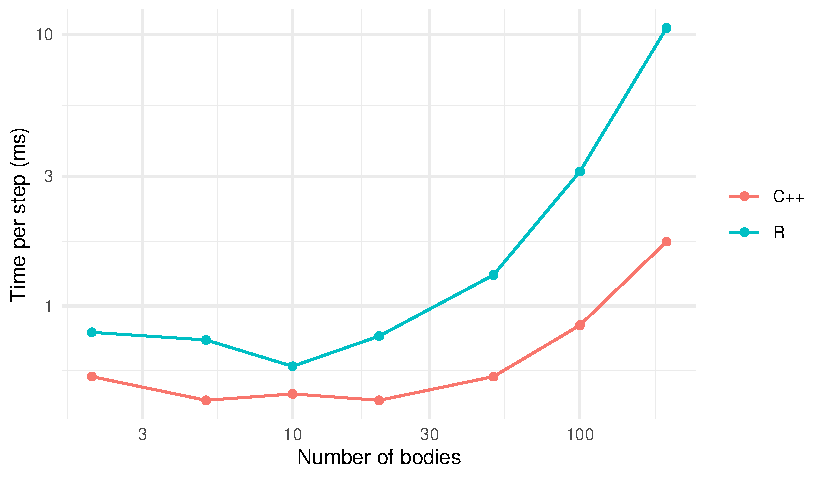
\includegraphics[width=1\linewidth,height=\textheight,keepaspectratio]{15-the-cpp-engine_files/figure-pdf/fig-bench-1.pdf}

}

\caption{\label{fig-bench}Milliseconds per integration step against the
number of bodies, for the C++ kernel and the R fallback, on the machine
this book was built on. Both axes are logarithmic. The flat part at
small \(n\) is the R loop's overhead; the rising part is the \(n^2\)
kernel.}

\end{figure}%

Read the C++ curve from the left. For two bodies and for twenty, the
time per step is about the same: that is the fixed cost of the R loop,
the tibble updates, and the call into the kernel, and it is independent
of \(n\). The kernel's \(n^2\) term is invisible until it grows to match
that overhead, somewhere around fifty bodies, after which the curve
bends up with slope 2 on the log-log plot: doubling \(n\) quadruples the
time. The R fallback has a higher floor, because \texttt{outer()} and
friends allocate matrices on every call, and reaches the \(n^2\) regime
sooner.

The other large cost is at the end. \texttt{bind\_rows()} on sixty
thousand small tibbles, which is what Chapter 8's run produced, is slow,
because each tibble has to be checked and copied:

\begin{Shaded}
\begin{Highlighting}[]
\NormalTok{one\_step }\OtherTok{\textless{}{-}} \FunctionTok{get\_bodies}\NormalTok{(}\FunctionTok{cluster}\NormalTok{(}\DecValTok{9}\NormalTok{))}
\NormalTok{pieces   }\OtherTok{\textless{}{-}} \FunctionTok{replicate}\NormalTok{(}\DecValTok{10000}\NormalTok{, one\_step, }\AttributeTok{simplify =} \ConstantTok{FALSE}\NormalTok{)}
\FunctionTok{system.time}\NormalTok{(}\FunctionTok{bind\_rows}\NormalTok{(pieces))[[}\StringTok{"elapsed"}\NormalTok{]]}
\CommentTok{\#\textgreater{} [1] 0.14}
\end{Highlighting}
\end{Shaded}

Scale that by six for a 60,000-step run. For long runs of small systems,
assembling the output tibble takes about as long as integrating it. The
lesson for a user is simple: the number of \emph{recorded} steps is what
you pay for, and it is also what sets the size of the output. A
simulation that records every hour for a century produces 876,000 rows
per body whether or not it needed to.

\begin{tcolorbox}[enhanced jigsaw, arc=.35mm, bottomrule=.15mm, bottomtitle=1mm, breakable, colback=white, colbacktitle=quarto-callout-note-color!10!white, colframe=quarto-callout-note-color-frame, coltitle=black, left=2mm, leftrule=.75mm, opacityback=0, opacitybacktitle=0.6, rightrule=.15mm, title={Where it comes from}, titlerule=0mm, toprule=.15mm, toptitle=1mm]

This split, a compiled inner kernel driven by an interpreted outer loop,
is how almost all scientific computing in R and Python is done, and the
trade-off is always the same. The interpreted layer is where the
flexibility lives: the tibble output, the three integrators selectable
by a string, the softening argument. The compiled layer is where the
\(n^2\) lives. The design is right as long as the compiled part
dominates for the problems you care about. orbitr's design assumption is
a few to a few dozen bodies, and for those the R layer is the
bottleneck, which is a sign that the kernel is doing its job.

\end{tcolorbox}

\section{\texorpdfstring{The \(n^2\)
wall}{The n\^{}2 wall}}\label{the-n2-wall}

Extrapolate the C++ curve. If the kernel costs \(c\,n^2\) per
evaluation, the \(n = 200\) point gives \(c\), and

\begin{Shaded}
\begin{Highlighting}[]
\NormalTok{c\_kernel }\OtherTok{\textless{}{-}}\NormalTok{ bench }\SpecialCharTok{|\textgreater{}} \FunctionTok{filter}\NormalTok{(engine }\SpecialCharTok{==} \StringTok{"C++"}\NormalTok{, n }\SpecialCharTok{==} \DecValTok{200}\NormalTok{) }\SpecialCharTok{|\textgreater{}} \FunctionTok{pull}\NormalTok{(ms\_per\_step) }\SpecialCharTok{/} \DecValTok{200}\SpecialCharTok{\^{}}\DecValTok{2}
\FunctionTok{tibble}\NormalTok{(}\AttributeTok{n =} \FunctionTok{c}\NormalTok{(}\FloatTok{1e3}\NormalTok{, }\FloatTok{1e4}\NormalTok{, }\FloatTok{1e5}\NormalTok{),}
       \AttributeTok{ms\_per\_step =}\NormalTok{ c\_kernel }\SpecialCharTok{*}\NormalTok{ n}\SpecialCharTok{\^{}}\DecValTok{2}\NormalTok{,}
       \AttributeTok{hours\_per\_10000\_steps =}\NormalTok{ ms\_per\_step }\SpecialCharTok{*} \FloatTok{1e4} \SpecialCharTok{/} \FloatTok{3.6e6}\NormalTok{)}
\CommentTok{\#\textgreater{} \# A tibble: 3 x 3}
\CommentTok{\#\textgreater{}        n ms\_per\_step hours\_per\_10000\_steps}
\CommentTok{\#\textgreater{}    \textless{}dbl\textgreater{}       \textless{}dbl\textgreater{}                 \textless{}dbl\textgreater{}}
\CommentTok{\#\textgreater{} 1   1000        43.1                 0.120}
\CommentTok{\#\textgreater{} 2  10000      4312.                 12.0  }
\CommentTok{\#\textgreater{} 3 100000    431250.               1198.}
\end{Highlighting}
\end{Shaded}

A thousand bodies is comfortable. Ten thousand is a long evening for a
short run. A hundred thousand is out of the question, and a galaxy has a
hundred billion stars. Research codes get around the wall in three ways:

\begin{itemize}
\tightlist
\item
  \textbf{Tree codes} (Barnes and Hut 1986) group distant bodies into
  cells and use each cell's center of mass instead of its members,
  reducing the cost to \(O(n\log n)\) at the price of a controllable
  approximation. Chapter 3's shell theorem is the justification: from
  far away, a clump of mass acts like a point.
\item
  \textbf{The fast multipole method} (Greengard and Rokhlin 1987) takes
  the idea further, expanding the potential of each cell in a series,
  and reaches \(O(n)\).
\item
  \textbf{Hardware.} The pairwise sum is embarrassingly parallel, and
  GPUs compute billions of pair interactions per second. Specialized
  hardware for exactly this sum, the GRAPE boards of the 1990s and
  2000s, was for a time the fastest computing in the world for anything.
\end{itemize}

orbitr does none of these, and it should not. Each of them is a large
piece of engineering whose approximation error has to be understood as
carefully as the integrator's, and none of them changes what a user of
this package wants: a tidy table of where a dozen bodies went. The tidy
table is itself the deeper limit. At \(n = 10^4\) bodies and \(10^4\)
steps the output is \(10^8\) rows, about seven gigabytes in memory, and
the data frame would fail before the kernel became the problem. Big
N-body simulation does not keep every position at every step; it writes
snapshots to disk and analyzes them later. That is a different kind of
tool.

\section{Changing the physics}\label{changing-the-physics}

Because every force the package computes is in one function, adding a
force is a small change to that function. A drag term proportional to
velocity would need the velocities passed in (three more
\texttt{NumericVector} arguments) and three lines inside the outer loop;
Earth's oblateness would need Earth identified and a dozen lines; the
relativistic correction of Chapter 16, a few more. None of it is hard,
and all of it is on the roadmap. If you want to try, the package is on
GitHub, \texttt{Rcpp::sourceCpp()} compiles a modified kernel in
seconds, and \texttt{simulate\_system()}'s \texttt{use\_cpp} argument is
the switch.

\begin{tcolorbox}[enhanced jigsaw, arc=.35mm, bottomrule=.15mm, bottomtitle=1mm, breakable, colback=white, colbacktitle=quarto-callout-tip-color!10!white, colframe=quarto-callout-tip-color-frame, coltitle=black, left=2mm, leftrule=.75mm, opacityback=0, opacitybacktitle=0.6, rightrule=.15mm, title={Key results}, titlerule=0mm, toprule=.15mm, toptitle=1mm]

\begin{itemize}
\tightlist
\item
  The entire physics is \texttt{calc\_acceleration\_cpp()}: a double
  loop over ordered pairs computing
  \(Gm_k(\mathbf{r}_k - \mathbf{r}_j)/r_{\mathrm{soft}}^3\). The R
  fallback is the same sum with \texttt{outer()} matrices.
\item
  For fewer than about fifty bodies, the R loop and the output assembly
  cost more than the kernel. The number of recorded steps, not the
  number of bodies, is what you pay for.
\item
  Beyond that, cost grows as \(n^2\); a thousand bodies is fine, a
  hundred thousand needs a different algorithm and a different output
  format.
\end{itemize}

\end{tcolorbox}

\chapter{Limits and Extensions}\label{sec-limits}

Chapter 1 listed what orbitr leaves out: bodies have no size, gravity is
Newtonian, there are no forces but gravity, and the step is fixed. This
chapter returns to each omission with the physics of what is missing,
the size of the effect, and what it would take to add it. Some of the
additions are on the package roadmap. Two of them you can do today with
the tools this book has built, and the chapter shows how. The rest are
described precisely enough that if you decide to implement one, you will
know what you are implementing.

\section{Collisions}\label{collisions}

Two point masses can pass through each other. Nothing in the equations
of motion objects, and if the step is small enough the integrator will
carry them straight through with energy conserved. In reality two
planets that pass within the sum of their radii collide. The package has
no notion of radius, so collisions are something you detect \emph{after}
the run, by looking.

A helper that finds the closest approach of every pair over a simulation
is a self-join on \texttt{time}, like Chapter 5's hand-written energy
sum:

\begin{Shaded}
\begin{Highlighting}[]
\NormalTok{closest\_approach }\OtherTok{\textless{}{-}} \ControlFlowTok{function}\NormalTok{(sim) \{}
\NormalTok{  sim }\SpecialCharTok{|\textgreater{}}
    \FunctionTok{select}\NormalTok{(time, id, x, y, z) }\SpecialCharTok{|\textgreater{}}
    \FunctionTok{inner\_join}\NormalTok{(sim }\SpecialCharTok{|\textgreater{}} \FunctionTok{select}\NormalTok{(time, }\AttributeTok{id2 =}\NormalTok{ id, }\AttributeTok{x2 =}\NormalTok{ x, }\AttributeTok{y2 =}\NormalTok{ y, }\AttributeTok{z2 =}\NormalTok{ z),}
               \AttributeTok{by =} \StringTok{"time"}\NormalTok{, }\AttributeTok{relationship =} \StringTok{"many{-}to{-}many"}\NormalTok{) }\SpecialCharTok{|\textgreater{}}
    \FunctionTok{filter}\NormalTok{(id }\SpecialCharTok{\textless{}}\NormalTok{ id2) }\SpecialCharTok{|\textgreater{}}
    \FunctionTok{mutate}\NormalTok{(}\AttributeTok{r =} \FunctionTok{sqrt}\NormalTok{((x }\SpecialCharTok{{-}}\NormalTok{ x2)}\SpecialCharTok{\^{}}\DecValTok{2} \SpecialCharTok{+}\NormalTok{ (y }\SpecialCharTok{{-}}\NormalTok{ y2)}\SpecialCharTok{\^{}}\DecValTok{2} \SpecialCharTok{+}\NormalTok{ (z }\SpecialCharTok{{-}}\NormalTok{ z2)}\SpecialCharTok{\^{}}\DecValTok{2}\NormalTok{)) }\SpecialCharTok{|\textgreater{}}
    \FunctionTok{group\_by}\NormalTok{(id, id2) }\SpecialCharTok{|\textgreater{}}
    \FunctionTok{slice\_min}\NormalTok{(r, }\AttributeTok{n =} \DecValTok{1}\NormalTok{) }\SpecialCharTok{|\textgreater{}}
    \FunctionTok{ungroup}\NormalTok{() }\SpecialCharTok{|\textgreater{}}
    \FunctionTok{select}\NormalTok{(id, id2, time, r)}
\NormalTok{\}}
\end{Highlighting}
\end{Shaded}

Run it on Chapter 11's chaotic triple, where the stars came within a
fraction of an AU of one another during the slingshot:

\begin{Shaded}
\begin{Highlighting}[]
\NormalTok{triple }\OtherTok{\textless{}{-}} \FunctionTok{create\_system}\NormalTok{() }\SpecialCharTok{|\textgreater{}}
  \FunctionTok{add\_body}\NormalTok{(}\StringTok{"Star A"}\NormalTok{, }\AttributeTok{mass =} \FloatTok{1e30}\NormalTok{, }\AttributeTok{x =} \FloatTok{1e11}\NormalTok{,  }\AttributeTok{y =} \DecValTok{0}\NormalTok{,        }\AttributeTok{vx =} \DecValTok{0}\NormalTok{,      }\AttributeTok{vy =} \DecValTok{15000}\NormalTok{) }\SpecialCharTok{|\textgreater{}}
  \FunctionTok{add\_body}\NormalTok{(}\StringTok{"Star B"}\NormalTok{, }\AttributeTok{mass =} \FloatTok{1e30}\NormalTok{, }\AttributeTok{x =} \SpecialCharTok{{-}}\FloatTok{5e10}\NormalTok{, }\AttributeTok{y =} \FloatTok{8.66e10}\NormalTok{,  }\AttributeTok{vx =} \SpecialCharTok{{-}}\DecValTok{12990}\NormalTok{, }\AttributeTok{vy =} \SpecialCharTok{{-}}\DecValTok{7500}\NormalTok{) }\SpecialCharTok{|\textgreater{}}
  \FunctionTok{add\_body}\NormalTok{(}\StringTok{"Star C"}\NormalTok{, }\AttributeTok{mass =} \FloatTok{1e30}\NormalTok{, }\AttributeTok{x =} \SpecialCharTok{{-}}\FloatTok{5e10}\NormalTok{, }\AttributeTok{y =} \SpecialCharTok{{-}}\FloatTok{8.66e10}\NormalTok{, }\AttributeTok{vx =} \DecValTok{14000}\NormalTok{,  }\AttributeTok{vy =} \SpecialCharTok{{-}}\DecValTok{8000}\NormalTok{) }\SpecialCharTok{|\textgreater{}}
  \FunctionTok{simulate\_system}\NormalTok{(}\AttributeTok{time\_step =}\NormalTok{ seconds\_per\_hour, }\AttributeTok{duration =}\NormalTok{ seconds\_per\_year }\SpecialCharTok{*} \DecValTok{3}\NormalTok{)}

\FunctionTok{closest\_approach}\NormalTok{(triple) }\SpecialCharTok{|\textgreater{}}
  \FunctionTok{mutate}\NormalTok{(}\AttributeTok{solar\_radii =}\NormalTok{ r }\SpecialCharTok{/} \FloatTok{6.957e8}\NormalTok{, }\AttributeTok{day =}\NormalTok{ time }\SpecialCharTok{/}\NormalTok{ seconds\_per\_day)}
\CommentTok{\#\textgreater{} \# A tibble: 3 x 6}
\CommentTok{\#\textgreater{}   id     id2        time            r solar\_radii   day}
\CommentTok{\#\textgreater{}   \textless{}chr\textgreater{}  \textless{}chr\textgreater{}     \textless{}dbl\textgreater{}        \textless{}dbl\textgreater{}       \textless{}dbl\textgreater{} \textless{}dbl\textgreater{}}
\CommentTok{\#\textgreater{} 1 Star A Star B  9288000 73615522151.       106.   108.}
\CommentTok{\#\textgreater{} 2 Star A Star C 82933200 20904109167.        30.0  960.}
\CommentTok{\#\textgreater{} 3 Star B Star C 10519200 61636240576.        88.6  122.}
\end{Highlighting}
\end{Shaded}

If any pair's closest approach is less than the sum of their radii (two
solar radii, for Sun-like stars), the simulation went somewhere reality
would not have, and everything after that time is fiction. The check
costs seconds and belongs at the end of every run involving close
encounters.

A real collision model needs a rule for what happens next. The usual
choice in planet-formation codes is a perfectly inelastic merger: the
two bodies become one with the summed mass, the center-of-mass position,
and the momentum-conserving velocity
\(\mathbf{v} = (m_1\mathbf{v}_1 + m_2\mathbf{v}_2)/(m_1+m_2)\). Momentum
is conserved; kinetic energy is not, and the difference is the energy
that goes into cratering and heat. The roadmap's \texttt{radius}
argument on \texttt{add\_body()} is the hook for this, and
\texttt{system\_from\_simulation()}, \texttt{remove\_body()},
\texttt{add\_body()}, and \texttt{continue\_simulation()} are enough to
do it by hand today: stop at the collision time, rebuild the system from
that snapshot, replace the two bodies with their merger, and continue.

\section{Forces other than gravity}\label{forces-other-than-gravity}

Every force the package knows is in the kernel of Chapter 15. Three
others matter in practice, and they behave very differently.

\subsection{Radiation pressure}\label{radiation-pressure}

Sunlight carries momentum, and a small body absorbing it feels a force
directed away from the Sun that falls off as \(1/r^2\), exactly like
gravity. For a body of mass \(m\) and cross-section \(A\) at distance
\(r\), \(F = L_\odot A/(4\pi r^2 c)\), where \(L_\odot\) is the Sun's
luminosity. Because it has the same \(r\)-dependence as gravity,
radiation pressure does not change the \emph{shape} of the orbit
equation at all; it just reduces the effective gravitational parameter:

\begin{equation}\protect\phantomsection\label{eq-beta}{
\mu_{\mathrm{eff}} = GM_\odot\,(1 - \beta), \qquad \beta = \frac{F_{\mathrm{rad}}}{F_{\mathrm{grav}}} = \frac{L_\odot A}{4\pi c\,GM_\odot\,m}.
}\end{equation}

\(\beta\) depends on \(A/m\), so it is tiny for a planet and large for
dust. For a sphere of density \(\rho\) and radius \(s\),
\(A/m = 3/(4\rho s)\), which works out to
\(\beta \approx 0.57/(\rho s)\) with \(\rho\) in g/cm\(^3\) and \(s\) in
microns: a micron-sized grain, rocky or icy, feels sunlight at a sizable
fraction of gravity.

Because the correction is just a rescaled \(\mu\), you can simulate it
today with the tool already in \texttt{create\_system()}. For a test
particle in orbit around the Sun alone, setting \(G \to G(1-\beta)\) is
exact. A grain released from a parent body on a circular orbit keeps the
parent's speed \(v = \sqrt{GM/r}\) but sees only \(\mu_{\mathrm{eff}}\);
by Chapter 4's rule, \(e = |k^2 - 1|\) with
\(k^2 = v^2/(\mu_{\mathrm{eff}}/r) = 1/(1-\beta)\), so

\[
e = \frac{\beta}{1-\beta},
\]

and the grain is unbound (\(e \ge 1\)) when \(\beta \ge 1/2\). Dust
released from a comet with \(\beta > 0.5\) leaves the solar system; that
is what the dust tail is.

\begin{Shaded}
\begin{Highlighting}[]
\NormalTok{grain }\OtherTok{\textless{}{-}} \ControlFlowTok{function}\NormalTok{(beta) \{}
  \FunctionTok{create\_system}\NormalTok{(}\AttributeTok{G =}\NormalTok{ gravitational\_constant }\SpecialCharTok{*}\NormalTok{ (}\DecValTok{1} \SpecialCharTok{{-}}\NormalTok{ beta)) }\SpecialCharTok{|\textgreater{}}
    \FunctionTok{add\_sun}\NormalTok{() }\SpecialCharTok{|\textgreater{}}
    \FunctionTok{add\_body}\NormalTok{(}\StringTok{"grain"}\NormalTok{, }\AttributeTok{mass =} \FloatTok{1e{-}12}\NormalTok{, }\AttributeTok{x =}\NormalTok{ distance\_earth\_sun, }\AttributeTok{vy =}\NormalTok{ speed\_earth) }\SpecialCharTok{|\textgreater{}}
    \FunctionTok{simulate\_system}\NormalTok{(}\AttributeTok{time\_step =}\NormalTok{ seconds\_per\_day, }\AttributeTok{duration =}\NormalTok{ seconds\_per\_year }\SpecialCharTok{*} \DecValTok{3}\NormalTok{) }\SpecialCharTok{|\textgreater{}}
    \FunctionTok{filter}\NormalTok{(id }\SpecialCharTok{==} \StringTok{"grain"}\NormalTok{) }\SpecialCharTok{|\textgreater{}}
    \FunctionTok{mutate}\NormalTok{(}\AttributeTok{beta =}\NormalTok{ beta)}
\NormalTok{\}}

\FunctionTok{bind\_rows}\NormalTok{(}\FunctionTok{grain}\NormalTok{(}\DecValTok{0}\NormalTok{), }\FunctionTok{grain}\NormalTok{(}\FloatTok{0.3}\NormalTok{), }\FunctionTok{grain}\NormalTok{(}\FloatTok{0.6}\NormalTok{)) }\SpecialCharTok{|\textgreater{}}
  \FunctionTok{ggplot}\NormalTok{(}\FunctionTok{aes}\NormalTok{(x }\SpecialCharTok{/}\NormalTok{ distance\_earth\_sun, y }\SpecialCharTok{/}\NormalTok{ distance\_earth\_sun,}
             \AttributeTok{color =} \FunctionTok{factor}\NormalTok{(beta))) }\SpecialCharTok{+}
  \FunctionTok{geom\_path}\NormalTok{() }\SpecialCharTok{+}
  \FunctionTok{annotate}\NormalTok{(}\StringTok{"point"}\NormalTok{, }\AttributeTok{x =} \DecValTok{0}\NormalTok{, }\AttributeTok{y =} \DecValTok{0}\NormalTok{, }\AttributeTok{size =} \DecValTok{3}\NormalTok{) }\SpecialCharTok{+}
  \FunctionTok{coord\_equal}\NormalTok{() }\SpecialCharTok{+}
  \FunctionTok{labs}\NormalTok{(}\AttributeTok{x =} \StringTok{"x (AU)"}\NormalTok{, }\AttributeTok{y =} \StringTok{"y (AU)"}\NormalTok{, }\AttributeTok{color =} \FunctionTok{expression}\NormalTok{(beta))}
\end{Highlighting}
\end{Shaded}

\begin{figure}[tbp]

\centering{

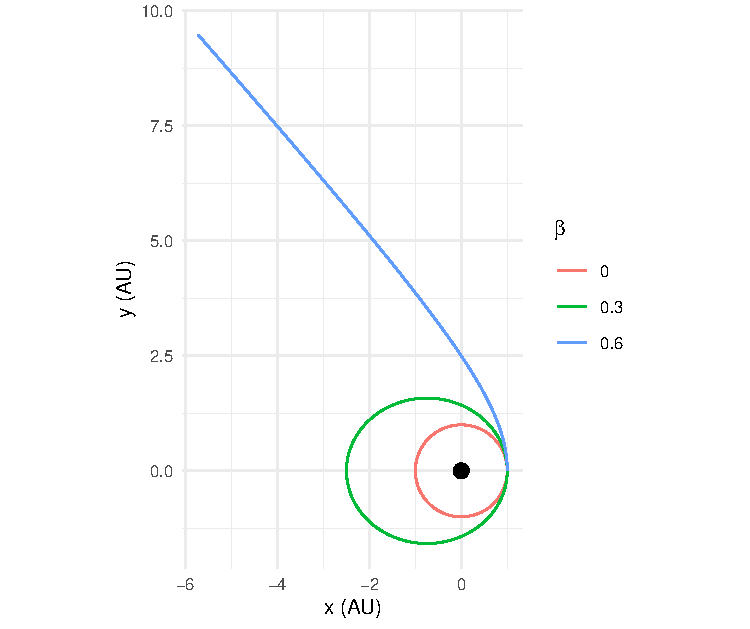
\includegraphics[width=0.7\linewidth,height=\textheight,keepaspectratio]{16-limits-and-extensions_files/figure-pdf/fig-radiation-pressure-1.pdf}

}

\caption{\label{fig-radiation-pressure}Three dust grains released from
Earth's orbit at Earth's speed, with radiation-pressure parameters
\(\beta\) of 0, 0.3, and 0.6, simulated by rescaling \(G\). The last is
unbound.}

\end{figure}%

The trick only works when the Sun is the only massive body. With planets
present, rescaling \(G\) would weaken their gravity too, and a proper
implementation adds the radiation force to the grain alone, inside the
kernel.

\subsection{Drag}\label{drag}

Atmospheric drag on a satellite is
\(\mathbf{F} = -\tfrac12 \rho(r)\, C_D A\, v\,\mathbf{v}\), opposing the
velocity and growing with the square of the speed and with the air
density, which falls off exponentially with altitude. It is dissipative:
it removes energy, and since \(\varepsilon = -\mu/2a\), removing energy
shrinks the orbit, which lowers the satellite into denser air, which
increases the drag. The decay accelerates until re-entry. The
International Space Station loses about two kilometers of altitude a
month to this and is periodically boosted.

Drag depends on velocity, which the kernel does not receive, so adding
it is a signature change as well as a few lines. But there is a way to
approximate it without touching the kernel, and it is a real numerical
technique: \emph{operator splitting}. Run gravity for a short interval
with \texttt{simulate\_system()}, then apply the drag as an
instantaneous change to the velocity, then run gravity again. Chapter
13's \texttt{continue\_simulation()} makes the loop a few lines. Here is
a toy satellite in an atmosphere with an artificially short damping
time, so that a year of decay fits in a figure:

\begin{Shaded}
\begin{Highlighting}[]
\NormalTok{kick\_drag }\OtherTok{\textless{}{-}} \ControlFlowTok{function}\NormalTok{(sim, body, tau, dt) \{}
\NormalTok{  last }\OtherTok{\textless{}{-}}\NormalTok{ sim}\SpecialCharTok{$}\NormalTok{time }\SpecialCharTok{==} \FunctionTok{max}\NormalTok{(sim}\SpecialCharTok{$}\NormalTok{time) }\SpecialCharTok{\&}\NormalTok{ sim}\SpecialCharTok{$}\NormalTok{id }\SpecialCharTok{==}\NormalTok{ body}
\NormalTok{  f }\OtherTok{\textless{}{-}} \FunctionTok{exp}\NormalTok{(}\SpecialCharTok{{-}}\NormalTok{dt }\SpecialCharTok{/}\NormalTok{ tau)                     }\CommentTok{\# velocity damping over the interval}
\NormalTok{  sim}\SpecialCharTok{$}\NormalTok{vx[last] }\OtherTok{\textless{}{-}}\NormalTok{ sim}\SpecialCharTok{$}\NormalTok{vx[last] }\SpecialCharTok{*}\NormalTok{ f}
\NormalTok{  sim}\SpecialCharTok{$}\NormalTok{vy[last] }\OtherTok{\textless{}{-}}\NormalTok{ sim}\SpecialCharTok{$}\NormalTok{vy[last] }\SpecialCharTok{*}\NormalTok{ f}
\NormalTok{  sim}\SpecialCharTok{$}\NormalTok{vz[last] }\OtherTok{\textless{}{-}}\NormalTok{ sim}\SpecialCharTok{$}\NormalTok{vz[last] }\SpecialCharTok{*}\NormalTok{ f}
\NormalTok{  sim}
\NormalTok{\}}

\NormalTok{sat }\OtherTok{\textless{}{-}} \FunctionTok{create\_system}\NormalTok{() }\SpecialCharTok{|\textgreater{}}
  \FunctionTok{add\_body}\NormalTok{(}\StringTok{"Earth"}\NormalTok{, }\AttributeTok{mass =}\NormalTok{ mass\_earth) }\SpecialCharTok{|\textgreater{}}
  \FunctionTok{add\_body}\NormalTok{(}\StringTok{"Sat"}\NormalTok{, }\AttributeTok{mass =} \FloatTok{1e3}\NormalTok{, }\AttributeTok{x =} \FloatTok{8e6}\NormalTok{, }\AttributeTok{vy =} \FunctionTok{sqrt}\NormalTok{(gravitational\_constant }\SpecialCharTok{*}\NormalTok{ mass\_earth }\SpecialCharTok{/} \FloatTok{8e6}\NormalTok{) }\SpecialCharTok{*} \FloatTok{1.1}\NormalTok{) }\SpecialCharTok{|\textgreater{}}
  \FunctionTok{simulate\_system}\NormalTok{(}\AttributeTok{time\_step =} \DecValTok{60}\NormalTok{, }\AttributeTok{duration =}\NormalTok{ seconds\_per\_day)}

\ControlFlowTok{for}\NormalTok{ (day }\ControlFlowTok{in} \DecValTok{1}\SpecialCharTok{:}\DecValTok{40}\NormalTok{) \{}
\NormalTok{  sat }\OtherTok{\textless{}{-}}\NormalTok{ sat }\SpecialCharTok{|\textgreater{}}
    \FunctionTok{kick\_drag}\NormalTok{(}\StringTok{"Sat"}\NormalTok{, }\AttributeTok{tau =} \DecValTok{200} \SpecialCharTok{*}\NormalTok{ seconds\_per\_day, }\AttributeTok{dt =}\NormalTok{ seconds\_per\_day) }\SpecialCharTok{|\textgreater{}}
    \FunctionTok{continue\_simulation}\NormalTok{(}\AttributeTok{time\_step =} \DecValTok{60}\NormalTok{, }\AttributeTok{duration =}\NormalTok{ seconds\_per\_day)}
\NormalTok{\}}

\NormalTok{sat }\SpecialCharTok{|\textgreater{}}
  \FunctionTok{filter}\NormalTok{(id }\SpecialCharTok{==} \StringTok{"Sat"}\NormalTok{) }\SpecialCharTok{|\textgreater{}}
  \FunctionTok{mutate}\NormalTok{(}\AttributeTok{r\_km =} \FunctionTok{sqrt}\NormalTok{(x}\SpecialCharTok{\^{}}\DecValTok{2} \SpecialCharTok{+}\NormalTok{ y}\SpecialCharTok{\^{}}\DecValTok{2}\NormalTok{) }\SpecialCharTok{/} \FloatTok{1e3}\NormalTok{) }\SpecialCharTok{|\textgreater{}}
  \FunctionTok{ggplot}\NormalTok{(}\FunctionTok{aes}\NormalTok{(time }\SpecialCharTok{/}\NormalTok{ seconds\_per\_day, r\_km)) }\SpecialCharTok{+}
  \FunctionTok{geom\_line}\NormalTok{() }\SpecialCharTok{+}
  \FunctionTok{labs}\NormalTok{(}\AttributeTok{x =} \StringTok{"Day"}\NormalTok{, }\AttributeTok{y =} \StringTok{"Distance from Earth\textquotesingle{}s center (km)"}\NormalTok{)}
\end{Highlighting}
\end{Shaded}

\begin{figure}[tbp]

\centering{

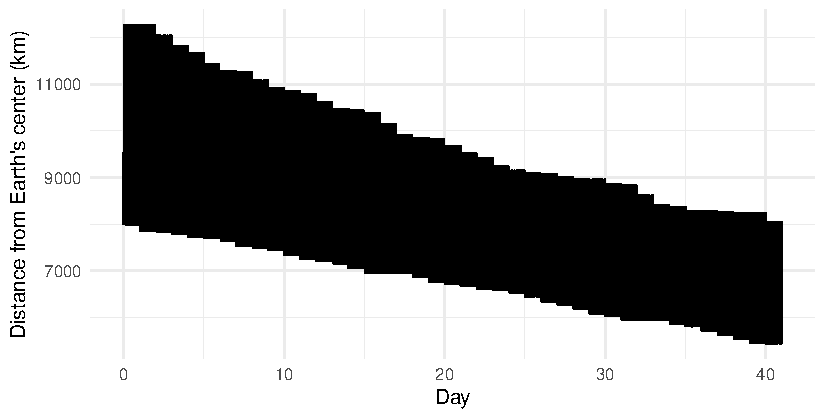
\includegraphics[width=1\linewidth,height=\textheight,keepaspectratio]{16-limits-and-extensions_files/figure-pdf/fig-drag-1.pdf}

}

\caption{\label{fig-drag}Orbital decay under a toy drag law applied by
operator splitting: gravity for a day, a small velocity kick, gravity
for a day. Energy leaves the orbit at every kick and the orbit shrinks.}

\end{figure}%

Splitting is first-order accurate in the interval between kicks, so make
the interval short compared with the drag timescale. The toy applies the
same fractional kick wherever the satellite happens to be, which is what
a body moving through a uniform medium feels. Real atmospheric drag is
concentrated at periapsis, where the air is densest, and that changes
the shape of the decay: periapsis stays nearly fixed while apoapsis is
pulled down, the orbit circularizes, and only then does the whole thing
spiral in. The same loop produces that behavior if the kick depends on
altitude through a density profile,
\(\tau(r) = \tau_0\exp\big((r - r_0)/H\big)\) with a scale height \(H\)
of about 60 km, applied every few minutes instead of every day.

\subsection{Thrust}\label{thrust}

A rocket burn is a kick too, and a short one is well modeled as an
instantaneous velocity change: a \(\Delta v\). The Hohmann transfer
between two circular orbits is two kicks, one at periapsis of the
transfer ellipse and one at apoapsis, with magnitudes that follow
directly from vis-viva: the transfer ellipse has \(a = (r_1 + r_2)/2\),
and each \(\Delta v\) is the difference between the circular speed and
the transfer-orbit speed at that radius. Splitting with
\texttt{continue\_simulation()} does it exactly.

\section{Oblateness}\label{oblateness}

Earth is not a sphere; it is an ellipsoid 21 km fatter at the equator
than at the poles, and the extra mass around the equator pulls a
satellite slightly off the point-mass orbit. The leading correction to
the potential is

\begin{equation}\protect\phantomsection\label{eq-j2}{
\Phi(r,\theta) = -\frac{GM}{r}\left[1 - J_2\left(\frac{R}{r}\right)^2\frac{3\cos^2\theta - 1}{2}\right],
}\end{equation}

where \(\theta\) is the angle from the rotation axis, \(R\) is the
equatorial radius, and \(J_2\) is a dimensionless number that measures
the bulge: \(1.083\times10^{-3}\) for Earth, \(14.7\times10^{-3}\) for
Jupiter, \(0.2\times10^{-3}\) for the Moon. The force is no longer
central, so angular momentum about the center is not conserved, and the
orbit's elements drift: the node \(\Omega\) regresses and the perigee
\(\omega\) advances, at rates that average to

\begin{equation}\protect\phantomsection\label{eq-j2-rates}{
\dot\Omega = -\frac{3}{2}\,n\,J_2\left(\frac{R}{a}\right)^2\frac{\cos i}{(1-e^2)^2}, \qquad
\dot\omega = \frac{3}{4}\,n\,J_2\left(\frac{R}{a}\right)^2\frac{5\cos^2 i - 1}{(1-e^2)^2},
}\end{equation}

with \(n = 2\pi/T\) the mean motion. For the International Space
Station:

\begin{Shaded}
\begin{Highlighting}[]
\NormalTok{R\_earth }\OtherTok{\textless{}{-}} \FloatTok{6.378e6}
\NormalTok{J2      }\OtherTok{\textless{}{-}} \FloatTok{1.083e{-}3}
\NormalTok{a\_iss   }\OtherTok{\textless{}{-}}\NormalTok{ R\_earth }\SpecialCharTok{+} \FloatTok{4.2e5}
\NormalTok{i\_iss   }\OtherTok{\textless{}{-}} \FloatTok{51.6} \SpecialCharTok{*}\NormalTok{ pi }\SpecialCharTok{/} \DecValTok{180}
\NormalTok{n\_iss   }\OtherTok{\textless{}{-}} \FunctionTok{sqrt}\NormalTok{(gravitational\_constant }\SpecialCharTok{*}\NormalTok{ mass\_earth }\SpecialCharTok{/}\NormalTok{ a\_iss}\SpecialCharTok{\^{}}\DecValTok{3}\NormalTok{)}

\NormalTok{node\_rate }\OtherTok{\textless{}{-}} \SpecialCharTok{{-}}\FloatTok{1.5} \SpecialCharTok{*}\NormalTok{ n\_iss }\SpecialCharTok{*}\NormalTok{ J2 }\SpecialCharTok{*}\NormalTok{ (R\_earth }\SpecialCharTok{/}\NormalTok{ a\_iss)}\SpecialCharTok{\^{}}\DecValTok{2} \SpecialCharTok{*} \FunctionTok{cos}\NormalTok{(i\_iss)}
\NormalTok{node\_rate }\SpecialCharTok{*}\NormalTok{ seconds\_per\_day }\SpecialCharTok{*} \DecValTok{180} \SpecialCharTok{/}\NormalTok{ pi        }\CommentTok{\# degrees per day}
\CommentTok{\#\textgreater{} [1] {-}4.952777}
\end{Highlighting}
\end{Shaded}

Five degrees a day. The ISS's orbital plane swings all the way around in
about ten weeks, which anyone who tracks its passes knows. A satellite
at an inclination near \(98°\) has \(\dot\Omega\) of exactly
\(+0.9856°\) per day, one full turn per year, so its orbital plane keeps
a fixed angle to the Sun: that is a Sun-synchronous orbit, and it is how
every Earth-observing satellite that needs constant lighting is flown.
All of it comes from the second term in Equation~\ref{eq-j2}, and all of
it is absent from a point-mass simulation. Adding it to the kernel means
giving one body an axis and a \(J_2\) and adding the gradient of the
correction term to the acceleration of everything near it.

\section{General relativity}\label{general-relativity}

Newtonian gravity gets Mercury's perihelion precession wrong by 43
arcseconds per century, and the discrepancy was known for half a century
before Einstein explained it. The general-relativistic correction to the
acceleration of a test body around a mass \(M\), to first post-Newtonian
order, is

\begin{equation}\protect\phantomsection\label{eq-1pn}{
\mathbf{a}_{\mathrm{GR}} = \frac{GM}{c^2 r^3}\left[\left(\frac{4GM}{r} - v^2\right)\mathbf{r} + 4\,(\mathbf{r}\cdot\mathbf{v})\,\mathbf{v}\right].
}\end{equation}

Its size relative to Newtonian gravity is of order \(v^2/c^2\), which
for Mercury is \(2\times10^{-8}\). Small, but it accumulates: the
perihelion advances by

\begin{equation}\protect\phantomsection\label{eq-gr-precession}{
\Delta\omega = \frac{6\pi GM}{c^2 a(1-e^2)}
}\end{equation}

per orbit, and Mercury makes 415 orbits a century:

\begin{Shaded}
\begin{Highlighting}[]
\NormalTok{c\_light }\OtherTok{\textless{}{-}} \FloatTok{2.998e8}
\NormalTok{a\_merc  }\OtherTok{\textless{}{-}}\NormalTok{ distance\_mercury\_sun}
\NormalTok{e\_merc  }\OtherTok{\textless{}{-}} \FloatTok{0.2056}
\NormalTok{per\_orbit }\OtherTok{\textless{}{-}} \DecValTok{6} \SpecialCharTok{*}\NormalTok{ pi }\SpecialCharTok{*}\NormalTok{ gravitational\_constant }\SpecialCharTok{*}\NormalTok{ mass\_sun }\SpecialCharTok{/}\NormalTok{ (c\_light}\SpecialCharTok{\^{}}\DecValTok{2} \SpecialCharTok{*}\NormalTok{ a\_merc }\SpecialCharTok{*}\NormalTok{ (}\DecValTok{1} \SpecialCharTok{{-}}\NormalTok{ e\_merc}\SpecialCharTok{\^{}}\DecValTok{2}\NormalTok{))}
\NormalTok{orbits\_per\_century }\OtherTok{\textless{}{-}} \DecValTok{100} \SpecialCharTok{*}\NormalTok{ seconds\_per\_year }\SpecialCharTok{/}\NormalTok{ (}\DecValTok{2} \SpecialCharTok{*}\NormalTok{ pi }\SpecialCharTok{*} \FunctionTok{sqrt}\NormalTok{(a\_merc}\SpecialCharTok{\^{}}\DecValTok{3} \SpecialCharTok{/}\NormalTok{ (gravitational\_constant }\SpecialCharTok{*}\NormalTok{ mass\_sun)))}

\NormalTok{per\_orbit }\SpecialCharTok{*}\NormalTok{ orbits\_per\_century }\SpecialCharTok{*} \DecValTok{180} \SpecialCharTok{/}\NormalTok{ pi }\SpecialCharTok{*} \DecValTok{3600}      \CommentTok{\# arcseconds per century}
\CommentTok{\#\textgreater{} [1] 42.99535}
\end{Highlighting}
\end{Shaded}

Forty-three arcseconds. Equation~\ref{eq-1pn} depends on velocity, like
drag, so it needs the same kernel signature change; it is about ten
lines of C++, and the roadmap lists it as an opt-in argument. Chapter 12
explained why measuring the result would be harder than implementing it:
the numerical precession at any practical step size is larger than the
relativistic one, and you would need the step small enough, or a smarter
integrator, to see 43 arcseconds under the artifact.

\section{Better integrators}\label{better-integrators}

Velocity Verlet with a fixed step is the right default and the wrong
tool for two situations this book has met: a highly eccentric orbit,
where the step should shrink near periapsis, and a long integration
where second-order accuracy is not enough.

\textbf{Adaptive steps} solve the first problem and create a new one. If
you change \(\Delta t\) based on the current state, the integrator is no
longer symplectic (the map from one step to the next is no longer a
fixed symplectic map), and the bounded-energy guarantee of Chapter 5 is
lost: the energy drifts secularly, just as Euler's does, though more
slowly. The fix is to choose the step \emph{time-symmetrically}, so that
the step size at each point is the same whether you arrive from the past
or the future; Hut, Makino, and McMillan showed how to do that with an
implicit iteration (Hut et al. 1995), and their time-symmetric leapfrog
is the ancestor of the block time steps that every modern star-cluster
code uses. Chapter 13's segmented runs are the crude version: a few
fixed-step symplectic segments with a small disturbance at each switch.

\textbf{Higher order} solves the second problem, and the symplectic way
to do it is composition. Yoshida showed in 1990 that three Verlet steps
of sizes \(w_1\Delta t\), \(w_0\Delta t\), \(w_1\Delta t\) with

\[
w_1 = \frac{1}{2 - 2^{1/3}} \approx 1.351, \qquad w_0 = -\frac{2^{1/3}}{2 - 2^{1/3}} \approx -1.702
\]

compose to a \emph{fourth}-order symplectic method (Yoshida 1990): halve
the step and the error drops by sixteen. The middle step is backward in
time, which looks absurd and is fine; it cancels the third-order error
of the two forward steps. The same construction yields sixth and eighth
order. (The package integrates only forward, so this is a
kernel-and-loop change, not a trick with
\texttt{continue\_simulation()}.)

\textbf{Non-symplectic high order} is the other route. IAS15 (Rein and
Spiegel 2015), the default integrator of the REBOUND code, is a
fifteenth-order adaptive scheme whose errors are below double-precision
rounding for a billion orbits; it gives up symplecticity and gets away
with it by being so accurate that there is no drift to speak of. For a
few bodies over a long time it is the state of the art. If you find
yourself needing it, that is the point at which to graduate from orbitr
to a research code, and you will understand what the research code is
doing.

\section{The roadmap, and how to
help}\label{the-roadmap-and-how-to-help}

The package roadmap, in the documentation under Roadmap, lists what is
being considered: a \texttt{radius} argument and collision handling;
drag, radiation pressure, \(J_2\), and the post-Newtonian correction as
optional forces; a progress bar for long runs; and built-in conservation
diagnostics. Three earlier items, Keplerian elements, the solar system
loader, and saving and loading systems, have already shipped, which is
some evidence that the list is not decorative.

If you want something that is not there, or want to build something that
is, the package is on GitHub at
\url{https://github.com/DRosenman/orbitr}. Open an issue to describe
what you need; a reproducible example, which in orbitr is usually five
lines, helps more than anything. If you implement a feature, every
chapter of this book is a test: the conservation laws of Chapter 12, the
two-body predictions of Chapter 4, the Kepler's-law check of Chapter 8.
A pull request that comes with the check that shows the physics is right
is the kind that gets merged.

\section{Where to go next}\label{where-to-go-next}

You now know what the simulation does and why. That is a different kind
of knowledge from knowing how to drive it, and it transfers. Every
orbital-mechanics code, from the ones that fly spacecraft to the ones
that model galaxy formation, is built from the same parts: a force law,
an integrator, a set of conserved quantities to watch, and a long list
of things left out. Some of them use the same integrator as orbitr. All
of them share its limits in one form or another, and the person who
understands the limits is the person who gets the right answer out of
the code.

Thornton and Marion (Thornton and Marion 2004) for the mechanics, Murray
and Dermott (Murray and Dermott 1999) for the solar system, Hairer,
Lubich, and Wanner (Hairer et al. 2006) for the integrators, and Aarseth
(Aarseth 2003) for the N-body methods will take you further than this
book did on each of its four parts. The package will keep changing. The
physics will not.

\begin{tcolorbox}[enhanced jigsaw, arc=.35mm, bottomrule=.15mm, bottomtitle=1mm, breakable, colback=white, colbacktitle=quarto-callout-tip-color!10!white, colframe=quarto-callout-tip-color-frame, coltitle=black, left=2mm, leftrule=.75mm, opacityback=0, opacitybacktitle=0.6, rightrule=.15mm, title={Key results}, titlerule=0mm, toprule=.15mm, toptitle=1mm]

\begin{itemize}
\tightlist
\item
  Collisions: detect after the run with \texttt{closest\_approach()}; a
  merger conserves momentum, not kinetic energy.
\item
  Radiation pressure rescales \(\mu\) by \((1-\beta)\); grains with
  \(\beta > 1/2\) escape. Drag and thrust are velocity kicks, which
  operator splitting with \texttt{continue\_simulation()} can apply
  today.
\item
  \(J_2\) regresses the node at \(-\tfrac32 n J_2 (R/a)^2\cos i\); five
  degrees a day for the ISS.
\item
  The post-Newtonian correction advances Mercury's perihelion by
  \(6\pi GM/(c^2 a(1-e^2))\) per orbit: 43 arcseconds per century.
\item
  Adaptive steps break symplecticity unless chosen time-symmetrically;
  higher order comes from Yoshida's composition of Verlet steps.
\end{itemize}

\end{tcolorbox}

\bookmarksetup{startatroot}

\chapter*{References}\label{references}
\addcontentsline{toc}{chapter}{References}

\markboth{References}{References}

\protect\phantomsection\label{refs}
\begin{CSLReferences}{1}{1}
\bibitem[\citeproctext]{ref-aarseth2003}
Aarseth, Sverre J. 2003. \emph{Gravitational {N}-Body Simulations: Tools
and Algorithms}. Cambridge University Press.

\bibitem[\citeproctext]{ref-barnes1986}
Barnes, Josh, and Piet Hut. 1986. {``A Hierarchical {O(N log N)}
Force-Calculation Algorithm.''} \emph{Nature} 324: 446--49.
\url{https://doi.org/10.1038/324446a0}.

\bibitem[\citeproctext]{ref-bate1971}
Bate, Roger R., Donald D. Mueller, and Jerry E. White. 1971.
\emph{Fundamentals of Astrodynamics}. Dover.

\bibitem[\citeproctext]{ref-cromer1981}
Cromer, Alan. 1981. {``Stable Solutions Using the {Euler}
Approximation.''} \emph{American Journal of Physics} 49 (5): 455--59.
\url{https://doi.org/10.1119/1.12478}.

\bibitem[\citeproctext]{ref-doyle2011}
{Doyle, Laurance R., Joshua A. Carter, Daniel C. Fabrycky, et al.} 2011.
{``{Kepler-16}: A Transiting Circumbinary Planet.''} \emph{Science} 333
(6049): 1602--6. \url{https://doi.org/10.1126/science.1210923}.

\bibitem[\citeproctext]{ref-eddelbuettel2011}
Eddelbuettel, Dirk, and Romain François. 2011. {``{Rcpp}: Seamless {R}
and {C++} Integration.''} \emph{Journal of Statistical Software} 40 (8):
1--18. \url{https://doi.org/10.18637/jss.v040.i08}.

\bibitem[\citeproctext]{ref-feynman1963}
Feynman, Richard P., Robert B. Leighton, and Matthew Sands. 1963.
\emph{The Feynman Lectures on Physics, Volume i}. Addison-Wesley.

\bibitem[\citeproctext]{ref-goldstein2002}
Goldstein, Herbert, Charles Poole, and John Safko. 2002. \emph{Classical
Mechanics}. 3rd ed. Addison-Wesley.

\bibitem[\citeproctext]{ref-greengard1987}
Greengard, Leslie, and Vladimir Rokhlin. 1987. {``A Fast Algorithm for
Particle Simulations.''} \emph{Journal of Computational Physics} 73 (2):
325--48. \url{https://doi.org/10.1016/0021-9991(87)90140-9}.

\bibitem[\citeproctext]{ref-hairer2003}
Hairer, Ernst, Christian Lubich, and Gerhard Wanner. 2003. {``Geometric
Numerical Integration Illustrated by the {St{ø}rmer--Verlet} Method.''}
\emph{Acta Numerica} 12: 399--450.
\url{https://doi.org/10.1017/S0962492902000144}.

\bibitem[\citeproctext]{ref-hairer2006}
Hairer, Ernst, Christian Lubich, and Gerhard Wanner. 2006.
\emph{Geometric Numerical Integration: Structure-Preserving Algorithms
for Ordinary Differential Equations}. 2nd ed. Springer.

\bibitem[\citeproctext]{ref-holman1999}
Holman, Matthew J., and Paul A. Wiegert. 1999. {``Long-Term Stability of
Planets in Binary Systems.''} \emph{The Astronomical Journal} 117 (1):
621--28. \url{https://doi.org/10.1086/300695}.

\bibitem[\citeproctext]{ref-hut1995}
Hut, Piet, Jun Makino, and Steve McMillan. 1995. {``Building a Better
Leapfrog.''} \emph{The Astrophysical Journal} 443: L93--96.
\url{https://doi.org/10.1086/187844}.

\bibitem[\citeproctext]{ref-kepler1609}
Kepler, Johannes. 1609. \emph{Astronomia Nova}. G. Voegelinus.

\bibitem[\citeproctext]{ref-kepler1619}
Kepler, Johannes. 1619. \emph{Harmonices Mundi}. J. Planck.

\bibitem[\citeproctext]{ref-murray1999}
Murray, Carl D., and Stanley F. Dermott. 1999. \emph{Solar System
Dynamics}. Cambridge University Press.

\bibitem[\citeproctext]{ref-newman2012}
Newman, Mark. 2012. \emph{Computational Physics}. CreateSpace.

\bibitem[\citeproctext]{ref-newton1687}
Newton, Isaac. 1687. \emph{Philosophi{æ} Naturalis Principia
Mathematica}. Royal Society.

\bibitem[\citeproctext]{ref-park2021}
Park, Ryan S., William M. Folkner, James G. Williams, and Dale H. Boggs.
2021. {``The {JPL} Planetary and Lunar Ephemerides {DE440} and
{DE441}.''} \emph{The Astronomical Journal} 161 (3): 105.
\url{https://doi.org/10.3847/1538-3881/abd414}.

\bibitem[\citeproctext]{ref-plummer1911}
Plummer, H. C. 1911. {``On the Problem of Distribution in Globular Star
Clusters.''} \emph{Monthly Notices of the Royal Astronomical Society} 71
(5): 460--70. \url{https://doi.org/10.1093/mnras/71.5.460}.

\bibitem[\citeproctext]{ref-poincare1890}
Poincaré, Henri. 1890. {``Sur Le Probl{è}me Des Trois Corps Et Les
{é}quations de La Dynamique.''} \emph{Acta Mathematica} 13: 1--270.
\url{https://doi.org/10.1007/BF02392506}.

\bibitem[\citeproctext]{ref-rein2015}
Rein, Hanno, and David S. Spiegel. 2015. {``{IAS15}: A Fast, Adaptive,
High-Order Integrator for Gravitational Dynamics, Accurate to Machine
Precision over a Billion Orbits.''} \emph{Monthly Notices of the Royal
Astronomical Society} 446 (2): 1424--37.
\url{https://doi.org/10.1093/mnras/stu2164}.

\bibitem[\citeproctext]{ref-rosenman2026orbitr}
Rosenman, David P. 2026. \emph{Orbitr: A Tidy Physics Engine for
Building and Visualizing Orbital Simulations in {R}}.
\url{https://orbit-r.com}.

\bibitem[\citeproctext]{ref-stormer1907}
Størmer, Carl. 1907. {``Sur Les Trajectoires Des Corpuscules
{é}lectris{é}s Dans l'espace Sous l'action Du Magn{é}tisme Terrestre,
Avec Application Aux Aurores Bor{é}ales.''} \emph{Archives Des Sciences
Physiques Et Naturelles} 24: 5--18, 113--58, 221--47.

\bibitem[\citeproctext]{ref-swope1982}
Swope, William C., Hans C. Andersen, Peter H. Berens, and Kent R.
Wilson. 1982. {``A Computer Simulation Method for the Calculation of
Equilibrium Constants for the Formation of Physical Clusters of
Molecules: Application to Small Water Clusters.''} \emph{The Journal of
Chemical Physics} 76 (1): 637--49.
\url{https://doi.org/10.1063/1.442716}.

\bibitem[\citeproctext]{ref-thornton2004}
Thornton, Stephen T., and Jerry B. Marion. 2004. \emph{Classical
Dynamics of Particles and Systems}. 5th ed. Brooks/Cole.

\bibitem[\citeproctext]{ref-tiesinga2021}
Tiesinga, Eite, Peter J. Mohr, David B. Newell, and Barry N. Taylor.
2021. {``{CODATA} Recommended Values of the Fundamental Physical
Constants: 2018.''} \emph{Reviews of Modern Physics} 93 (2): 025010.
\url{https://doi.org/10.1103/RevModPhys.93.025010}.

\bibitem[\citeproctext]{ref-touboul2022}
{Touboul, Pierre, Gilles Métris, Manuel Rodrigues, et al.} 2022.
{``{MICROSCOPE} Mission: Final Results of the Test of the Equivalence
Principle.''} \emph{Physical Review Letters} 129 (12): 121102.
\url{https://doi.org/10.1103/PhysRevLett.129.121102}.

\bibitem[\citeproctext]{ref-verlet1967}
Verlet, Loup. 1967. {``Computer {`Experiments'} on Classical Fluids.
{I}. {Thermodynamical} Properties of {Lennard-Jones} Molecules.''}
\emph{Physical Review} 159 (1): 98--103.
\url{https://doi.org/10.1103/PhysRev.159.98}.

\bibitem[\citeproctext]{ref-yoshida1990}
Yoshida, Haruo. 1990. {``Construction of Higher Order Symplectic
Integrators.''} \emph{Physics Letters A} 150 (5--7): 262--68.
\url{https://doi.org/10.1016/0375-9601(90)90092-3}.

\end{CSLReferences}

\cleardoublepage
\phantomsection
\addcontentsline{toc}{part}{Appendices}
\appendix

\chapter{R Basics}\label{sec-r-basics}

This appendix is for the reader who has never opened R. It covers the
minimum needed to run and modify the code in this book: installing the
software, running code, installing packages, and the small vocabulary of
functions the chapters use over and over. It is deliberately brief. R is
a large language and this book uses a narrow slice of it; the last
section says where to go when you want the rest, and every book listed
there is free online.

If you already use R, skip this. If you have used Python or MATLAB, skim
it; most of what differs is in the sections on the pipe and on tibbles.

\section{Installing R and RStudio}\label{installing-r-and-rstudio}

Two installs, in this order.

\textbf{R} is the language. Download it from
\url{https://cran.r-project.org}: pick your operating system, then the
``base'' distribution on Windows or the \texttt{.pkg} installer on a
Mac, and run the installer with its defaults. On Linux, use your
distribution's package manager (\texttt{sudo\ apt\ install\ r-base} on
Ubuntu).

\textbf{RStudio} is the editor most people use, and the one this book
assumes. Download the free desktop version from
\url{https://posit.co/download/rstudio-desktop/}. (Positron, from the
same company, is a newer alternative; either works.) When you open
RStudio you will see four panes. The two that matter now are the
\textbf{Console} at the bottom left, where you type a line of R and get
an answer, and the \textbf{Source} pane above it, where you edit files.

Try the console. Type \texttt{2\ +\ 2} next to the
\texttt{\textgreater{}} prompt and press Enter:

\begin{Shaded}
\begin{Highlighting}[]
\DecValTok{2} \SpecialCharTok{+} \DecValTok{2}
\CommentTok{\#\textgreater{} [1] 4}
\end{Highlighting}
\end{Shaded}

The \texttt{{[}1{]}} means ``this is the first element of the result,''
which matters once results have more than one element, and they usually
do.

\section{Running code}\label{running-code}

Three ways, from quickest to most reusable.

\begin{itemize}
\tightlist
\item
  \textbf{Console.} Type and press Enter. Good for checking something.
\item
  \textbf{Script.} File → New File → R Script gives you a text file
  ending in \texttt{.R}. Type lines of code; press Ctrl+Enter (Cmd+Enter
  on a Mac) to run the line the cursor is on, or select several lines
  and press it to run them together. Save the file and you can rerun
  everything tomorrow.
\item
  \textbf{Quarto or R Markdown document.} A document that mixes text and
  code ``chunks,'' which is what this book is written in. File → New
  File → Quarto Document. Each chunk has a small green arrow to run it.
  This is the right format for a lab report, because the figures and
  numbers are regenerated from the code every time you render.
\end{itemize}

Lines starting with \texttt{\#} are comments and are ignored. Assignment
uses \texttt{\textless{}-}: \texttt{x\ \textless{}-\ 3} stores the value
3 under the name \texttt{x}, and typing \texttt{x} afterward prints it.
(\texttt{=} also works for assignment; \texttt{\textless{}-} is the
convention and the book uses it.)

\begin{Shaded}
\begin{Highlighting}[]
\NormalTok{x }\OtherTok{\textless{}{-}} \DecValTok{3}
\NormalTok{x }\SpecialCharTok{*} \DecValTok{2}
\CommentTok{\#\textgreater{} [1] 6}
\end{Highlighting}
\end{Shaded}

Everything in R is case-sensitive: \texttt{mass\_earth} and
\texttt{Mass\_Earth} are different names, and only the first one exists.

\section{Packages}\label{packages}

R's base installation is small on purpose. Almost everything useful,
including orbitr, comes as a \textbf{package}, which you install once
and load each session.

\begin{Shaded}
\begin{Highlighting}[]
\FunctionTok{install.packages}\NormalTok{(}\StringTok{"orbitr"}\NormalTok{)      }\CommentTok{\# once, downloads and installs (needs internet)}
\FunctionTok{library}\NormalTok{(orbitr)                 }\CommentTok{\# every session, makes the functions available}
\end{Highlighting}
\end{Shaded}

\texttt{install.packages()} takes the name in quotes; \texttt{library()}
takes it bare (quotes work there too). If you call a function from a
package you have not loaded, R says
\texttt{could\ not\ find\ function\ "simulate\_system"}, and the fix is
\texttt{library(orbitr)}. Installing orbitr also installs dplyr and
ggplot2, which the book uses for analysis and plotting; load them the
same way. The preface's ``What you need'' section has the full list,
including how to get the development version from GitHub.

Two more things about packages. \texttt{packageVersion("orbitr")} tells
you which version you have; this book needs 1.0.0 or later. And
\texttt{orbitr::simulate\_system()}, with the double colon, calls a
function from a package without loading the whole package, which is why
you will see \texttt{tidyr::pivot\_longer()} in a few places in the book
for a package that is used only once.

\section{Getting help}\label{getting-help}

\texttt{?simulate\_system} opens the help page for a function: what it
does, every argument and its default, and runnable examples at the
bottom. This is the single most useful habit to form. Every function in
orbitr has one, and Appendix~\ref{sec-function-reference} is a condensed
index of them. For a package as a whole, its website
(\url{https://orbit-r.com} for orbitr) has longer articles than the help
pages.

When something goes wrong, read the error message from the top; the
first line usually says what R could not do, and the rest is where it
was when it failed. The three errors new users hit most are
\texttt{could\ not\ find\ function} (load the package),
\texttt{object\ \textquotesingle{}x\textquotesingle{}\ not\ found} (you
have not created \texttt{x} yet, or spelled it differently), and
\texttt{unexpected\ symbol} or
\texttt{unexpected\ \textquotesingle{})\textquotesingle{}} (a typo: a
missing comma, an extra bracket, mismatched quotes). RStudio's editor
underlines the last kind in red before you run it.

\section{Functions and arguments}\label{functions-and-arguments}

A function call is a name followed by parentheses with the inputs,
called arguments, inside:

\begin{Shaded}
\begin{Highlighting}[]
\FunctionTok{sqrt}\NormalTok{(}\DecValTok{16}\NormalTok{)}
\CommentTok{\#\textgreater{} [1] 4}
\FunctionTok{round}\NormalTok{(}\FloatTok{3.14159}\NormalTok{, }\AttributeTok{digits =} \DecValTok{2}\NormalTok{)}
\CommentTok{\#\textgreater{} [1] 3.14}
\end{Highlighting}
\end{Shaded}

Arguments can be matched by position or by name.
\texttt{round(3.14159,\ 2)} and \texttt{round(3.14159,\ digits\ =\ 2)}
are the same call. This book names arguments almost everywhere, because
\texttt{add\_body("Moon",\ mass\ =\ mass\_moon,\ x\ =\ distance\_earth\_moon,\ vy\ =\ speed\_moon)}
is readable and the positional version is not. Arguments with defaults
can be left out: \texttt{add\_body()} has \texttt{x}, \texttt{y},
\texttt{z}, \texttt{vx}, \texttt{vy}, and \texttt{vz} all defaulting to
0, so you only mention the ones that are not zero.

Writing your own function is the same idea in reverse:

\begin{Shaded}
\begin{Highlighting}[]
\NormalTok{circular\_speed }\OtherTok{\textless{}{-}} \ControlFlowTok{function}\NormalTok{(mass, r, }\AttributeTok{G =}\NormalTok{ gravitational\_constant) \{}
  \FunctionTok{sqrt}\NormalTok{(G }\SpecialCharTok{*}\NormalTok{ mass }\SpecialCharTok{/}\NormalTok{ r)}
\NormalTok{\}}

\FunctionTok{circular\_speed}\NormalTok{(mass\_earth, distance\_earth\_moon)}
\CommentTok{\#\textgreater{} [1] 1018.289}
\end{Highlighting}
\end{Shaded}

The body runs with the arguments filled in, and the last value computed
is returned. The book defines a dozen small functions like this; every
one of them follows this pattern.

\section{The pipe}\label{the-pipe}

Most of the book's code is written as a chain:

\begin{Shaded}
\begin{Highlighting}[]
\FunctionTok{create\_system}\NormalTok{() }\SpecialCharTok{|\textgreater{}}
  \FunctionTok{add\_sun}\NormalTok{() }\SpecialCharTok{|\textgreater{}}
  \FunctionTok{add\_planet}\NormalTok{(}\StringTok{"Earth"}\NormalTok{, }\AttributeTok{parent =} \StringTok{"Sun"}\NormalTok{) }\SpecialCharTok{|\textgreater{}}
  \FunctionTok{simulate\_system}\NormalTok{(}\AttributeTok{time\_step =}\NormalTok{ seconds\_per\_day, }\AttributeTok{duration =}\NormalTok{ seconds\_per\_year) }\SpecialCharTok{|\textgreater{}}
  \FunctionTok{plot\_orbits}\NormalTok{()}
\end{Highlighting}
\end{Shaded}

The operator \texttt{\textbar{}\textgreater{}} is the \textbf{pipe}. It
takes the value on its left and passes it as the \emph{first argument}
of the function on its right, so
\texttt{x\ \textbar{}\textgreater{}\ f(y)} means \texttt{f(x,\ y)}. The
chain above is exactly

\begin{Shaded}
\begin{Highlighting}[]
\FunctionTok{plot\_orbits}\NormalTok{(}\FunctionTok{simulate\_system}\NormalTok{(}\FunctionTok{add\_planet}\NormalTok{(}\FunctionTok{add\_sun}\NormalTok{(}\FunctionTok{create\_system}\NormalTok{()), }\StringTok{"Earth"}\NormalTok{, }\AttributeTok{parent =} \StringTok{"Sun"}\NormalTok{),}
                            \AttributeTok{time\_step =}\NormalTok{ seconds\_per\_day, }\AttributeTok{duration =}\NormalTok{ seconds\_per\_year))}
\end{Highlighting}
\end{Shaded}

which says the same thing inside out and is why nobody writes it that
way. Read a pipe top to bottom as a sequence of steps: create a system,
add the Sun, add Earth, simulate, plot. Each function in orbitr takes
the system or the simulation output as its first argument precisely so
that it can sit in a chain like this.

You will see \texttt{\%\textgreater{}\%} in older code and in some of
the books below; it is the same idea from the magrittr package, from
before the pipe was built into R. \texttt{\textbar{}\textgreater{}}
needs R 4.1 or later, which is why the preface asks for it.

\section{Vectors, data frames, and
tibbles}\label{vectors-data-frames-and-tibbles}

A \textbf{vector} is a sequence of values of one type, built with
\texttt{c()}:

\begin{Shaded}
\begin{Highlighting}[]
\NormalTok{speeds }\OtherTok{\textless{}{-}} \FunctionTok{c}\NormalTok{(}\DecValTok{1000}\NormalTok{, }\DecValTok{1022}\NormalTok{, }\DecValTok{1044}\NormalTok{)}
\NormalTok{speeds }\SpecialCharTok{*} \DecValTok{2}
\CommentTok{\#\textgreater{} [1] 2000 2044 2088}
\NormalTok{speeds[}\DecValTok{2}\NormalTok{]}
\CommentTok{\#\textgreater{} [1] 1022}
\end{Highlighting}
\end{Shaded}

Arithmetic applies to every element at once, with no loop, and
\texttt{{[}2{]}} picks the second element. Most of R works this way,
which is why the book's code has so few loops.

A \textbf{data frame} is a table: columns are vectors, all the same
length, each with a name. A \textbf{tibble} is the modern data frame,
from the tidyverse, with a tidier print method and fewer surprises.
Everything orbitr returns is a tibble. The output of
\texttt{simulate\_system()} has one row per body per time step and the
columns \texttt{time}, \texttt{id}, \texttt{mass}, \texttt{x},
\texttt{y}, \texttt{z}, \texttt{vx}, \texttt{vy}, \texttt{vz}:

\begin{Shaded}
\begin{Highlighting}[]
\NormalTok{sim }\OtherTok{\textless{}{-}} \FunctionTok{create\_system}\NormalTok{() }\SpecialCharTok{|\textgreater{}}
  \FunctionTok{add\_body}\NormalTok{(}\StringTok{"Earth"}\NormalTok{, }\AttributeTok{mass =}\NormalTok{ mass\_earth) }\SpecialCharTok{|\textgreater{}}
  \FunctionTok{add\_body}\NormalTok{(}\StringTok{"Moon"}\NormalTok{, }\AttributeTok{mass =}\NormalTok{ mass\_moon, }\AttributeTok{x =}\NormalTok{ distance\_earth\_moon, }\AttributeTok{vy =}\NormalTok{ speed\_moon) }\SpecialCharTok{|\textgreater{}}
  \FunctionTok{simulate\_system}\NormalTok{(}\AttributeTok{time\_step =}\NormalTok{ seconds\_per\_hour, }\AttributeTok{duration =}\NormalTok{ seconds\_per\_day }\SpecialCharTok{*} \DecValTok{2}\NormalTok{)}

\NormalTok{sim}
\CommentTok{\#\textgreater{} \# A tibble: 98 x 9}
\CommentTok{\#\textgreater{}    id       mass          x           y     z      vx          vy    vz  time}
\CommentTok{\#\textgreater{}    \textless{}chr\textgreater{}   \textless{}dbl\textgreater{}      \textless{}dbl\textgreater{}       \textless{}dbl\textgreater{} \textless{}dbl\textgreater{}   \textless{}dbl\textgreater{}       \textless{}dbl\textgreater{} \textless{}dbl\textgreater{} \textless{}dbl\textgreater{}}
\CommentTok{\#\textgreater{}  1 Earth 5.97e24         0         0        0   0        0            0     0}
\CommentTok{\#\textgreater{}  2 Moon  7.34e22 384400000         0        0   0     1022            0     0}
\CommentTok{\#\textgreater{}  3 Earth 5.97e24       215.        0        0   0.119    0.000571     0  3600}
\CommentTok{\#\textgreater{}  4 Moon  7.34e22 384382520.  3679200        0  {-}9.71  1022.           0  3600}
\CommentTok{\#\textgreater{}  5 Earth 5.97e24       860.        4.11     0   0.239    0.00229      0  7200}
\CommentTok{\#\textgreater{}  6 Moon  7.34e22 384330083.  7358065.       0 {-}19.4   1022.           0  7200}
\CommentTok{\#\textgreater{}  7 Earth 5.97e24      1934.       16.5      0   0.358    0.00514      0 10800}
\CommentTok{\#\textgreater{}  8 Moon  7.34e22 384242692. 11036262.       0 {-}29.1   1022.           0 10800}
\CommentTok{\#\textgreater{}  9 Earth 5.97e24      3438.       41.1      0   0.477    0.00914      0 14400}
\CommentTok{\#\textgreater{} 10 Moon  7.34e22 384120357. 14713454.       0 {-}38.8   1021.           0 14400}
\CommentTok{\#\textgreater{} \# i 88 more rows}
\end{Highlighting}
\end{Shaded}

Printing a tibble shows the first ten rows and the column types
(\texttt{\textless{}chr\textgreater{}} is text,
\texttt{\textless{}dbl\textgreater{}} is a number). \texttt{nrow(sim)}
and \texttt{names(sim)} give the row count and the column names;
\texttt{sim\$x} pulls one column out as a plain vector;
\texttt{sim{[}sim\$id\ ==\ "Moon",\ {]}} picks rows by a condition. The
dplyr verbs in the next section do the same things more readably, and
the book uses them instead.

\section{The six dplyr verbs the book
uses}\label{the-six-dplyr-verbs-the-book-uses}

dplyr is the tidyverse package for working with tables, and the book
uses six of its functions. Each takes a tibble as its first argument (so
it sits in a pipe) and returns a tibble.

\begin{Shaded}
\begin{Highlighting}[]
\FunctionTok{library}\NormalTok{(dplyr)}

\NormalTok{sim }\SpecialCharTok{|\textgreater{}}
  \FunctionTok{filter}\NormalTok{(id }\SpecialCharTok{==} \StringTok{"Moon"}\NormalTok{) }\SpecialCharTok{|\textgreater{}}                      \CommentTok{\# keep rows where this is true}
  \FunctionTok{mutate}\NormalTok{(}\AttributeTok{r\_km =} \FunctionTok{sqrt}\NormalTok{(x}\SpecialCharTok{\^{}}\DecValTok{2} \SpecialCharTok{+}\NormalTok{ y}\SpecialCharTok{\^{}}\DecValTok{2} \SpecialCharTok{+}\NormalTok{ z}\SpecialCharTok{\^{}}\DecValTok{2}\NormalTok{) }\SpecialCharTok{/} \FloatTok{1e3}\NormalTok{) }\SpecialCharTok{|\textgreater{}} \CommentTok{\# add a column computed from others}
  \FunctionTok{select}\NormalTok{(time, r\_km) }\SpecialCharTok{|\textgreater{}}                        \CommentTok{\# keep only these columns}
  \FunctionTok{arrange}\NormalTok{(}\FunctionTok{desc}\NormalTok{(r\_km)) }\SpecialCharTok{|\textgreater{}}                       \CommentTok{\# sort rows (desc = largest first)}
  \FunctionTok{slice\_head}\NormalTok{(}\AttributeTok{n =} \DecValTok{3}\NormalTok{)                            }\CommentTok{\# the first few rows}
\CommentTok{\#\textgreater{} \# A tibble: 3 x 2}
\CommentTok{\#\textgreater{}     time    r\_km}
\CommentTok{\#\textgreater{}    \textless{}dbl\textgreater{}   \textless{}dbl\textgreater{}}
\CommentTok{\#\textgreater{} 1 172800 384673.}
\CommentTok{\#\textgreater{} 2 169200 384662.}
\CommentTok{\#\textgreater{} 3 165600 384652.}
\end{Highlighting}
\end{Shaded}

The one that takes a moment to learn is \texttt{summarise()} with
\texttt{group\_by()}: split the table into groups, then collapse each
group to one row.

\begin{Shaded}
\begin{Highlighting}[]
\NormalTok{sim }\SpecialCharTok{|\textgreater{}}
  \FunctionTok{group\_by}\NormalTok{(id) }\SpecialCharTok{|\textgreater{}}
  \FunctionTok{summarise}\NormalTok{(}\AttributeTok{max\_speed =} \FunctionTok{max}\NormalTok{(}\FunctionTok{sqrt}\NormalTok{(vx}\SpecialCharTok{\^{}}\DecValTok{2} \SpecialCharTok{+}\NormalTok{ vy}\SpecialCharTok{\^{}}\DecValTok{2} \SpecialCharTok{+}\NormalTok{ vz}\SpecialCharTok{\^{}}\DecValTok{2}\NormalTok{)),}
            \AttributeTok{n\_steps   =} \FunctionTok{n}\NormalTok{())}
\CommentTok{\#\textgreater{} \# A tibble: 2 x 3}
\CommentTok{\#\textgreater{}   id    max\_speed n\_steps}
\CommentTok{\#\textgreater{}   \textless{}chr\textgreater{}     \textless{}dbl\textgreater{}   \textless{}int\textgreater{}}
\CommentTok{\#\textgreater{} 1 Earth      5.68      49}
\CommentTok{\#\textgreater{} 2 Moon    1022         49}
\end{Highlighting}
\end{Shaded}

Inside any of these, column names are used bare, without quotes or
\texttt{sim\$}: \texttt{filter(id\ ==\ "Moon")}, not
\texttt{filter(sim\$id\ ==\ "Moon")}. Comparisons use \texttt{==} for
equals, \texttt{!=} for not equals, and \texttt{\&}, \texttt{\textbar{}}
for and, or. That is nearly all the dplyr in the book;
\texttt{inner\_join()}, which lines up two tables on a shared column,
appears in a few chapters and is explained where it is used.

\section{The ggplot2 the book uses}\label{the-ggplot2-the-book-uses}

ggplot2 builds a plot in layers. You say which columns map to which
visual properties (\texttt{aes()}), add a geometry layer that draws
them, and keep adding with \texttt{+}:

\begin{Shaded}
\begin{Highlighting}[]
\FunctionTok{library}\NormalTok{(ggplot2)}

\NormalTok{sim }\SpecialCharTok{|\textgreater{}}
  \FunctionTok{filter}\NormalTok{(id }\SpecialCharTok{==} \StringTok{"Moon"}\NormalTok{) }\SpecialCharTok{|\textgreater{}}
  \FunctionTok{mutate}\NormalTok{(}\AttributeTok{r\_km =} \FunctionTok{sqrt}\NormalTok{(x}\SpecialCharTok{\^{}}\DecValTok{2} \SpecialCharTok{+}\NormalTok{ y}\SpecialCharTok{\^{}}\DecValTok{2} \SpecialCharTok{+}\NormalTok{ z}\SpecialCharTok{\^{}}\DecValTok{2}\NormalTok{) }\SpecialCharTok{/} \FloatTok{1e3}\NormalTok{) }\SpecialCharTok{|\textgreater{}}
  \FunctionTok{ggplot}\NormalTok{(}\FunctionTok{aes}\NormalTok{(}\AttributeTok{x =}\NormalTok{ time }\SpecialCharTok{/}\NormalTok{ seconds\_per\_hour, }\AttributeTok{y =}\NormalTok{ r\_km)) }\SpecialCharTok{+}
  \FunctionTok{geom\_line}\NormalTok{() }\SpecialCharTok{+}
  \FunctionTok{labs}\NormalTok{(}\AttributeTok{x =} \StringTok{"Hour"}\NormalTok{, }\AttributeTok{y =} \StringTok{"Distance from origin (km)"}\NormalTok{)}
\end{Highlighting}
\end{Shaded}

\begin{center}
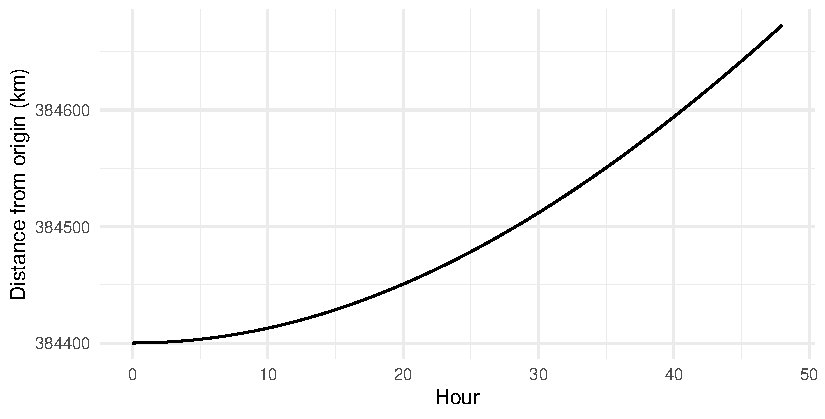
\includegraphics[width=1\linewidth,height=\textheight,keepaspectratio]{A-r-basics_files/figure-pdf/unnamed-chunk-13-1.pdf}
\end{center}

Note the switch from \texttt{\textbar{}\textgreater{}} to \texttt{+}
once the plot starts: ggplot2 predates the pipe and uses \texttt{+} to
add layers. The geometries the book uses are \texttt{geom\_line()} (a
line in order of \(x\)), \texttt{geom\_path()} (a line in the order of
the rows, which is what an orbit needs), \texttt{geom\_point()}, and
\texttt{annotate("point",\ ...)} for a single marker.
\texttt{aes(color\ =\ id)} colors by a column and adds a legend
automatically. \texttt{facet\_wrap(\textasciitilde{}\ method)} splits
one plot into panels, one per value of a column. \texttt{coord\_equal()}
makes one meter on the \(x\) axis the same length as one meter on \(y\),
without which circles come out as ellipses, and
\texttt{scale\_y\_log10()} gives a logarithmic axis. \texttt{labs()}
sets the labels and \texttt{theme\_minimal()} the look.
\texttt{plot\_orbits()} returns a ggplot built this way, so anything
here can be added to it.

\section{Where to learn more}\label{where-to-learn-more}

All of these are free to read online, and all are good.

\begin{itemize}
\tightlist
\item
  \textbf{R for Data Science}, by Hadley Wickham, Mine Çetinkaya-Rundel,
  and Garrett Grolemund (\url{https://r4ds.hadley.nz}). The standard
  introduction to the tidyverse: dplyr, ggplot2, tibbles, and the way of
  working this book assumes. If you read one other book, read this one;
  the first few chapters are enough.
\item
  \textbf{Hands-On Programming with R}, by Garrett Grolemund
  (\url{https://rstudio-education.github.io/hopr/}). Shorter and more
  about the language itself: vectors, functions, loops, the things R4DS
  skips. Good if you want to understand \emph{why} R behaves as it does.
\item
  \textbf{ggplot2: Elegant Graphics for Data Analysis}, by Hadley
  Wickham, Danielle Navarro, and Thomas Lin Pedersen
  (\url{https://ggplot2-book.org}). The full account of the plotting
  system, from the people who wrote it. Read it when
  \texttt{plot\_orbits()} stops being enough.
\item
  \textbf{R Graphics Cookbook}, by Winston Chang
  (\url{https://r-graphics.org}). Recipes: ``I want a plot that looks
  like this.'' The fastest route to a specific figure.
\item
  \textbf{Advanced R}, by Hadley Wickham
  (\url{https://adv-r.hadley.nz}). Not needed for this book. Read it
  when you start wanting to know what a function \emph{is}.
\item
  The \textbf{Posit cheat sheets}
  (\url{https://posit.co/resources/cheatsheets/}). One page each for
  dplyr, ggplot2, and RStudio; worth printing.
\end{itemize}

For the physics side, the references in the chapters and the Further
Reading section at \url{https://orbit-r.com} do the same job.

\chapter{Mathematical Background}\label{sec-math}

This appendix collects the mathematics the rest of the book takes for
granted. It is not a course; it is a reference, written for a reader who
has met calculus and vectors before and wants the specific facts the
derivations lean on, in the notation the book uses, with a pointer to
where each one earns its keep. If you can read it without surprises, you
have everything you need. If a section is new to you, it is short enough
to learn from, and the chapter it feeds will make it concrete.

The book assumes you are comfortable with algebra, with trigonometry
(sines, cosines, radians), and with the derivative and integral of a
function of one variable. Everything beyond that is here.

\section{Vectors}\label{vectors}

A \textbf{vector} is a quantity with magnitude and direction: a
position, a velocity, a force. The book sets vectors in bold,
\(\mathbf{r}\), and writes their components as
\(\mathbf{r} = (x, y, z)\). The \textbf{magnitude} (length) is

\[
r = |\mathbf{r}| = \sqrt{x^2 + y^2 + z^2},
\]

in italic, and the \textbf{unit vector} in the direction of
\(\mathbf{r}\) wears a hat, \(\hat{\mathbf{r}} = \mathbf{r}/r\), with
\(|\hat{\mathbf{r}}| = 1\). Vectors add component by component, and
multiplying a vector by a number scales its length (and reverses it if
the number is negative). The difference \(\mathbf{r}_k - \mathbf{r}_j\)
is the vector \emph{from} \(\mathbf{r}_j\) \emph{to} \(\mathbf{r}_k\);
its magnitude is the distance between the two points. That one fact is
the whole content of Chapter 3's force law.

\subsection{The dot product}\label{the-dot-product}

The \textbf{dot product} of two vectors is a number:

\begin{equation}\protect\phantomsection\label{eq-dot}{
\mathbf{a}\cdot\mathbf{b} = a_x b_x + a_y b_y + a_z b_z = |\mathbf{a}|\,|\mathbf{b}|\cos\theta,
}\end{equation}

where \(\theta\) is the angle between them. It is commutative
(\(\mathbf{a}\cdot\mathbf{b} = \mathbf{b}\cdot\mathbf{a}\)), distributes
over addition, and is zero when the vectors are perpendicular. Two uses
recur throughout the book. First, a vector dotted with itself is its
squared length, \(\mathbf{r}\cdot\mathbf{r} = r^2\), which is how the
book gets from vector equations to scalar ones (Chapter 4's energy
derivation). Second, the dot product with a unit vector picks out the
component along that direction: \(\mathbf{v}\cdot\hat{\mathbf{r}}\) is
the part of the velocity that points radially.

\subsection{The cross product}\label{the-cross-product}

The \textbf{cross product} of two vectors is a vector:

\begin{equation}\protect\phantomsection\label{eq-cross}{
\mathbf{a}\times\mathbf{b} = \big(a_y b_z - a_z b_y,\ a_z b_x - a_x b_z,\ a_x b_y - a_y b_x\big).
}\end{equation}

Its magnitude is \(|\mathbf{a}|\,|\mathbf{b}|\sin\theta\), which is the
area of the parallelogram the two vectors span (so
\(\tfrac12|\mathbf{a}\times\mathbf{b}|\) is the area of the triangle;
Chapter 4 uses this for Kepler's second law). Its direction is
perpendicular to both \(\mathbf{a}\) and \(\mathbf{b}\), by the
right-hand rule: curl the fingers of your right hand from \(\mathbf{a}\)
toward \(\mathbf{b}\) and the thumb points along
\(\mathbf{a}\times\mathbf{b}\). The properties the book uses:

\begin{itemize}
\tightlist
\item
  It is \textbf{anticommutative}:
  \(\mathbf{b}\times\mathbf{a} = -\mathbf{a}\times\mathbf{b}\).
\item
  Any vector crossed with itself, or with a multiple of itself, is zero:
  \(\mathbf{a}\times\mathbf{a} = \mathbf{0}\),
  \(\mathbf{a}\times(c\mathbf{a}) = \mathbf{0}\). This is why angular
  momentum is conserved under a central force (Chapter 4).
\item
  It distributes over addition and obeys the product rule under
  differentiation (next section).
\end{itemize}

Angular momentum, \(\mathbf{r}\times\mathbf{v}\), is the cross product
you will see most. The pattern of indices in Equation~\ref{eq-cross} is
worth memorizing once: each component uses the other two coordinates,
cyclically (\(x \to y \to z \to x\)), and the code in Chapters 4, 7, and
12 is a direct transcription of it.

\subsection{Two triple-product
identities}\label{two-triple-product-identities}

Chapter 4's derivation of the orbit equation uses two identities for
three vectors.

The \textbf{scalar triple product}
\(\mathbf{a}\cdot(\mathbf{b}\times\mathbf{c})\) is the volume of the
parallelepiped spanned by the three, and it is unchanged by cycling the
vectors:

\begin{equation}\protect\phantomsection\label{eq-scalar-triple}{
\mathbf{a}\cdot(\mathbf{b}\times\mathbf{c}) = \mathbf{b}\cdot(\mathbf{c}\times\mathbf{a}) = \mathbf{c}\cdot(\mathbf{a}\times\mathbf{b}).
}\end{equation}

It is zero if any two of the vectors are parallel or if all three lie in
a plane. The book uses it to turn
\(\mathbf{r}\cdot(\mathbf{v}\times\mathbf{h})\) into
\(\mathbf{h}\cdot(\mathbf{r}\times\mathbf{v}) = h^2\).

The \textbf{vector triple product} expands as

\begin{equation}\protect\phantomsection\label{eq-vector-triple}{
\mathbf{a}\times(\mathbf{b}\times\mathbf{c}) = \mathbf{b}\,(\mathbf{a}\cdot\mathbf{c}) - \mathbf{c}\,(\mathbf{a}\cdot\mathbf{b}),
}\end{equation}

the ``BAC minus CAB'' rule. Note that the result lies in the plane of
\(\mathbf{b}\) and \(\mathbf{c}\), and that the parentheses matter:
\((\mathbf{a}\times\mathbf{b})\times\mathbf{c}\) is a different vector.
Both identities can be verified by writing out components with
Equation~\ref{eq-cross}; it is tedious once and then you never doubt
them again.

\section{Derivatives of vectors}\label{derivatives-of-vectors}

A vector that changes with time is differentiated component by
component: if \(\mathbf{r}(t) = (x(t), y(t), z(t))\) then
\(\dot{\mathbf{r}} = (\dot x, \dot y, \dot z)\). The book uses Newton's
dot for time derivatives: \(\dot{\mathbf{r}}\) is velocity,
\(\ddot{\mathbf{r}}\) is acceleration. Velocity is also written
\(\mathbf{v}\) and acceleration \(\mathbf{a}\) when the context is
clear.

The product rules work for every kind of product, as long as the order
of the factors is kept in the cross product:

\begin{equation}\protect\phantomsection\label{eq-vector-product-rules}{
\frac{d}{dt}(f\mathbf{a}) = \dot f\,\mathbf{a} + f\,\dot{\mathbf{a}}, \qquad
\frac{d}{dt}(\mathbf{a}\cdot\mathbf{b}) = \dot{\mathbf{a}}\cdot\mathbf{b} + \mathbf{a}\cdot\dot{\mathbf{b}}, \qquad
\frac{d}{dt}(\mathbf{a}\times\mathbf{b}) = \dot{\mathbf{a}}\times\mathbf{b} + \mathbf{a}\times\dot{\mathbf{b}}.
}\end{equation}

Two consequences do a lot of work in Chapter 4.

\textbf{The derivative of a length.} Differentiating
\(r^2 = \mathbf{r}\cdot\mathbf{r}\) gives
\(2r\dot r = 2\,\mathbf{r}\cdot\dot{\mathbf{r}}\), so

\begin{equation}\protect\phantomsection\label{eq-r-dot}{
\dot r = \frac{\mathbf{r}\cdot\dot{\mathbf{r}}}{r} = \hat{\mathbf{r}}\cdot\dot{\mathbf{r}}.
}\end{equation}

The rate at which the distance changes is the radial component of the
velocity. Note that \(\dot r\) (the derivative of the length) is not
\(|\dot{\mathbf{r}}|\) (the length of the derivative, the speed); on a
circular orbit the first is zero and the second is not.

\textbf{The derivative of a unit vector.} By the quotient rule and
Equation~\ref{eq-r-dot},

\begin{equation}\protect\phantomsection\label{eq-unit-vector-dot}{
\frac{d}{dt}\left(\frac{\mathbf{r}}{r}\right) = \frac{\dot{\mathbf{r}}}{r} - \frac{\mathbf{r}\,\dot r}{r^2} = \frac{\dot{\mathbf{r}}}{r} - \frac{\mathbf{r}\,(\mathbf{r}\cdot\dot{\mathbf{r}})}{r^3}.
}\end{equation}

This is the expression that the vector triple product produces in
Chapter 4's eccentricity-vector derivation, and recognizing it is the
step that makes the derivation close.

A function of a vector, like the potential \(-\mu/r\), is differentiated
through the chain rule: \(\frac{d}{dt}(-\mu/r) = \mu\dot r/r^2\), and
then Equation~\ref{eq-r-dot}.

\section{Polar coordinates in the
plane}\label{polar-coordinates-in-the-plane}

Two-body orbits are planar (Chapter 4 proves it), so most of the book's
geometry lives in a plane, where a point can be given either by
Cartesian coordinates \((x, y)\) or by its distance \(r\) from the
origin and its angle \(\theta\) from the \(x\) axis:

\[
x = r\cos\theta, \qquad y = r\sin\theta, \qquad r = \sqrt{x^2+y^2}, \qquad \theta = \operatorname{atan2}(y, x).
\]

The orbit equation of Chapter 4 is a relation between \(r\) and
\(\theta\). To differentiate it you need the velocity in polar form.
Define the unit vectors \(\hat{\mathbf{r}} = (\cos\theta, \sin\theta)\),
pointing outward, and
\(\hat{\boldsymbol{\theta}} = (-\sin\theta, \cos\theta)\), pointing in
the direction of increasing \(\theta\). Unlike the Cartesian unit
vectors, these rotate as the point moves:
\(\dot{\hat{\mathbf{r}}} = \dot\theta\,\hat{\boldsymbol{\theta}}\) and
\(\dot{\hat{\boldsymbol{\theta}}} = -\dot\theta\,\hat{\mathbf{r}}\).
Differentiating \(\mathbf{r} = r\hat{\mathbf{r}}\) with the product
rule,

\begin{equation}\protect\phantomsection\label{eq-polar-velocity}{
\mathbf{v} = \dot r\,\hat{\mathbf{r}} + r\dot\theta\,\hat{\boldsymbol{\theta}}.
}\end{equation}

The velocity has a radial part, \(\dot r\), and a transverse part,
\(r\dot\theta\), and the speed squared is
\(\dot r^2 + r^2\dot\theta^2\). The angular momentum per unit mass is
\(h = |\mathbf{r}\times\mathbf{v}| = r\cdot r\dot\theta = r^2\dot\theta\),
and because \(h\) is constant for a central force this gives
\(\dot\theta = h/r^2\) directly, which Chapter 7 uses to turn the orbit
equation into the velocity formulas. In a time \(dt\) the position
vector sweeps out a thin triangle of area
\(\tfrac12 r\cdot r\dot\theta\,dt\), so the area swept per unit time is
\(h/2\): Kepler's second law in one line.

\section{Conic sections}\label{conic-sections}

Every two-body orbit is a conic section: the curve you get by slicing a
cone with a plane. Chapter 4 derives this; here is the geometry it
needs.

An \textbf{ellipse} is the set of points whose distances to two fixed
points, the \textbf{foci}, add up to a constant, \(2a\). It has a
longest diameter \(2a\) (the major axis) and a shortest \(2b\) (the
minor axis); \(a\) is the \textbf{semi-major axis} and \(b\) the
\textbf{semi-minor axis}. The foci lie on the major axis at a distance
\(c = \sqrt{a^2 - b^2}\) from the center, and the \textbf{eccentricity}
is \(e = c/a\), between 0 (a circle, both foci at the center) and 1 (a
degenerate line). The relations the book uses:

\begin{equation}\protect\phantomsection\label{eq-ellipse-facts}{
b = a\sqrt{1-e^2}, \qquad \text{area} = \pi a b, \qquad r_{\min} = a(1-e), \qquad r_{\max} = a(1+e),
}\end{equation}

where \(r_{\min}\) and \(r_{\max}\) are the nearest and farthest
distances from a focus (periapsis and apoapsis, when the focus is a
star). With the origin at one focus and \(\nu\) the angle from the
direction of the nearest point, the ellipse is

\begin{equation}\protect\phantomsection\label{eq-conic-polar}{
r(\nu) = \frac{a(1-e^2)}{1 + e\cos\nu} = \frac{p}{1 + e\cos\nu},
}\end{equation}

where \(p = a(1-e^2)\) is the \textbf{semi-latus rectum}, the distance
from the focus to the curve at \(\nu = 90°\). Check it: \(\nu = 0\)
gives \(a(1-e)\) and \(\nu = \pi\) gives \(a(1+e)\). This polar form is
the one that falls out of Newton's law, and it is why the orbiting body
is at a focus rather than at the center.

The same equation with \(e = 1\) describes a \textbf{parabola}, which
reaches infinity at \(\nu = \pm 180°\), and with \(e > 1\) a
\textbf{hyperbola}, which reaches infinity at the \textbf{asymptotes}
\(\nu = \pm\arccos(-1/e)\); between them the denominator is positive and
the curve is a single open branch. For a hyperbola the semi-major axis
is conventionally negative, \(a < 0\), so that \(p = a(1-e^2) > 0\) and
the periapsis distance \(a(1-e) > 0\) come out right from the same
formulas. The angle between the two asymptotes, which is how much a
flyby bends a trajectory, is \(2\arcsin(1/e)\). Chapter 13 uses all of
this.

\section{Taylor series}\label{taylor-series}

If a function is smooth, its value a short distance ahead can be built
from its derivatives at the current point:

\begin{equation}\protect\phantomsection\label{eq-taylor-general}{
f(t + \Delta t) = f(t) + f'(t)\,\Delta t + \frac{f''(t)}{2}\,\Delta t^2 + \frac{f'''(t)}{6}\,\Delta t^3 + \cdots
}\end{equation}

The general term is \(f^{(n)}(t)\,\Delta t^n/n!\). For the position of a
body this reads
\(\mathbf{r}(t+\Delta t) = \mathbf{r} + \mathbf{v}\Delta t + \tfrac12\mathbf{a}\Delta t^2 + \cdots\),
which is where every integrator in Chapter 5 comes from: an integrator
is a decision about where to cut the series off and what to do about the
terms you cut.

The \textbf{big-O} notation summarizes the size of what was cut. Writing
``\(+\,O(\Delta t^3)\)'' means the omitted terms are no larger than a
constant times \(\Delta t^3\) when \(\Delta t\) is small. The practical
meaning is in the scaling: an \(O(\Delta t^3)\) error shrinks by a
factor of eight when the step is halved, an \(O(\Delta t^2)\) error by
four. If a method's error over one step is \(O(\Delta t^{p+1})\), then
over a fixed time interval, which takes \(1/\Delta t\) steps, the
accumulated error is \(O(\Delta t^p)\), and the method is said to be of
order \(p\). Chapter 5 measures these exponents directly.

Three special cases of Equation~\ref{eq-taylor-general} appear so often
that it is worth knowing them by sight, with \(x\) small:

\begin{equation}\protect\phantomsection\label{eq-common-approximations}{
(1 + x)^n \approx 1 + nx, \qquad \sin x \approx x, \qquad e^x \approx 1 + x.
}\end{equation}

The first, the \textbf{binomial approximation}, is how Chapter 6
estimates the cost of softening:
\((1 + \varepsilon^2/r^2)^{-3/2} \approx 1 - \tfrac32\,\varepsilon^2/r^2\).
The last is how a small growth rate turns into exponential growth over
many steps: multiplying by \((1 + x)\) a total of \(N\) times gives
\((1+x)^N \approx e^{Nx}\).

\section{Differential equations and the idea of
state}\label{differential-equations-and-the-idea-of-state}

Newton's second law for one body,
\(\ddot{\mathbf{r}} = \mathbf{a}(\mathbf{r})\), is a
\textbf{second-order differential equation}: it involves the second
derivative of the unknown function \(\mathbf{r}(t)\). To solve it you
need two pieces of starting information, the position and the velocity
at some instant, because the equation only tells you how the velocity
\emph{changes}. Those two pieces are the \textbf{state}, and the whole
of Chapter 3's ``simulation loop'' is the observation that a
second-order equation can be rewritten as two first-order ones,

\[
\dot{\mathbf{r}} = \mathbf{v}, \qquad \dot{\mathbf{v}} = \mathbf{a}(\mathbf{r}),
\]

each of which says how one part of the state changes given the current
state. Any system of higher-order equations can be reduced to first
order this way, and numerical methods work on the first-order form.

A \textbf{solution in closed form} is a formula for \(\mathbf{r}(t)\).
The simplest example is the harmonic oscillator,
\(\ddot x = -\omega^2 x\), whose solution is
\(x(t) = A\cos\omega t + B\sin\omega t\), with \(A\) and \(B\) fixed by
the initial position and velocity. Chapter 5 uses this equation as its
test case because it is exactly solvable, so an integrator's mistakes
can be measured against the truth. The two-body problem has a
closed-form solution too (Chapter 4). The three-body problem does not
(Chapter 11), and the simulation is the only way to find
\(\mathbf{r}(t)\).

A \textbf{conserved quantity} (or first integral) is a function of the
state that does not change along any solution, like the oscillator's
energy \(\tfrac12\dot x^2 + \tfrac12\omega^2 x^2\). Finding one is the
standard trick for learning about a solution without solving: Chapter 4
finds three for the two-body problem and reads the shape of the orbit
off them.

\section{Matrices, rotations, and
determinants}\label{matrices-rotations-and-determinants}

A \textbf{matrix} is a grid of numbers; a \(2\times2\) or \(3\times3\)
matrix acts on a vector to produce another vector, by the rule ``each
component of the output is the dot product of a row with the input'':

\[
\begin{pmatrix} a & b \\ c & d \end{pmatrix}\begin{pmatrix} x \\ y \end{pmatrix} = \begin{pmatrix} ax + by \\ cx + dy \end{pmatrix}.
\]

Applying one matrix after another is the same as applying their
\textbf{product}, and the product is read right to left: \(M_2 M_1\)
applies \(M_1\) first. Matrix multiplication is not commutative, which
is why the order of the three rotations in Chapter 7 matters.

A \textbf{rotation} of the plane counterclockwise by \(\theta\) is the
matrix

\[
R(\theta) = \begin{pmatrix} \cos\theta & -\sin\theta \\ \sin\theta & \cos\theta \end{pmatrix},
\]

and the three-dimensional rotations about the \(z\) and \(x\) axes are
this block embedded in the \(3\times3\) identity:

\begin{equation}\protect\phantomsection\label{eq-rotation-matrices}{
R_z(\theta) = \begin{pmatrix} \cos\theta & -\sin\theta & 0 \\ \sin\theta & \cos\theta & 0 \\ 0 & 0 & 1 \end{pmatrix}, \qquad
R_x(\theta) = \begin{pmatrix} 1 & 0 & 0 \\ 0 & \cos\theta & -\sin\theta \\ 0 & \sin\theta & \cos\theta \end{pmatrix}.
}\end{equation}

Rotations preserve lengths and angles. Their inverse is their transpose
(\(R^{-1} = R^{T}\)), so undoing a rotation costs nothing. The sign
convention here, that \(R(\theta)\) rotates the \emph{vector}
counterclockwise by \(\theta\), is the one the package uses; some texts
instead rotate the coordinate axes, which is the same matrix with
\(-\theta\).

The \textbf{determinant} of a \(2\times2\) matrix is \(ad - bc\). Its
geometric meaning is the thing Chapter 5 is built on: a matrix with
determinant \(D\) scales every area by a factor \(|D|\) (every volume,
for \(3\times3\) matrices). A rotation has determinant 1, as it should.
A map that preserves area has determinant exactly 1, and a map with
determinant greater than 1 inflates every region it touches. Chapter 5
computes the determinant of each integrator's one-step map and finds
\(1 + \omega^2\Delta t^2\) for Euler and exactly 1 for Euler-Cromer and
Verlet; that single number is the difference between an orbit that
spirals and one that does not.

One more fact about \(2\times2\) matrices, used in a Chapter 5 exercise:
the eigenvalues \(\lambda\) satisfy
\(\lambda^2 - (\operatorname{trace})\lambda + \det = 0\). When
\(\det = 1\) the two eigenvalues multiply to 1, and they are a
complex-conjugate pair on the unit circle, meaning the map rotates
without growing, exactly when \(|\operatorname{trace}| < 2\). That is
where the stability condition \(\omega\Delta t < 2\) comes from.

\section{Logarithms, exponentials, and power
laws}\label{logarithms-exponentials-and-power-laws}

If \(y = C x^k\), then \(\log y = \log C + k\log x\): a power law is a
straight line on a plot with logarithmic axes, and its slope is the
exponent. Chapter 8 checks Kepler's third law this way (the slope is
\(3/2\)) and Chapter 15 reads the \(n^2\) cost of the force calculation
off a log-log benchmark. Chapter 5's convergence tables are the same
idea in a table: halving \(\Delta t\) and watching the error fall by
\(2^p\) measures \(p\).

If a quantity grows as \(y = y_0\,e^{t/\tau}\), then \(\log y\) is a
straight line against \(t\) with slope \(1/\tau\); \(\tau\) is the
\textbf{e-folding time}, the time for the quantity to grow by a factor
of \(e \approx 2.718\). Chapter 11 measures the Lyapunov time of a
chaotic triple, and the instability time of a Lagrange point, from
exactly such a slope. The natural logarithm is the one that makes this
work; R's \texttt{log()} is natural by default, and \texttt{log10()} is
for the axes.

\section{Angles}\label{angles}

The book's formulas use \textbf{radians}; the package's arguments use
\textbf{degrees}, because that is how orbital elements are published.
The conversion is \(\pi\) radians \(= 180°\), so multiply degrees by
\(\pi/180\) to get radians, and the book's code does this at the top of
every function that takes an angle.

The angle of a point \((x, y)\) from the \(x\) axis is
\texttt{atan2(y,\ x)}, not \texttt{atan(y/x)}: the two-argument form
knows which quadrant the point is in and returns a value in
\((-\pi, \pi]\). The jump from \(+\pi\) to \(-\pi\) as a body crosses
the negative \(x\) axis is an artifact of that range, and several
chapters \textbf{unwrap} a sequence of angles, adding \(2\pi\) at each
jump so the angle grows continuously and a body's total travel can be
measured. The helper \texttt{unwrap()} in \texttt{R/helpers.R} does this
with one line: take successive differences, wrap each into
\((-\pi, \pi]\), and accumulate.

\section{Units and dimensions}\label{units-and-dimensions}

Everything in the book is in SI units: meters, kilograms, seconds. The
only reason to mention it is that \textbf{dimensional analysis} is the
cheapest error check there is, and the book uses it silently all the
time. \(G\) has units \(\mathrm{m^3\,kg^{-1}\,s^{-2}}\), so \(GM\) has
units \(\mathrm{m^3\,s^{-2}}\), \(GM/r\) has units
\(\mathrm{m^2\,s^{-2}}\), and \(\sqrt{GM/r}\) has units of
\(\mathrm{m\,s^{-1}}\): a speed, as the circular-orbit formula says it
should be. \(\sqrt{a^3/GM}\) has units of seconds, so
\(2\pi\sqrt{a^3/\mu}\) is a time, as Kepler's third law requires. If you
derive a formula and the units do not come out right, the formula is
wrong; if they do, it is at worst wrong by a dimensionless factor like
\(2\pi\), which is the kind of error a simulation will show you
immediately.

A related habit is estimating \textbf{orders of magnitude} before
computing. Earth's orbital speed is
\(\sqrt{GM_\odot/r} \approx \sqrt{1.3\times10^{20}/1.5\times10^{11}} \approx \sqrt{10^9} \approx 3\times10^4\)
m/s. Knowing that number is about 30 km/s before you run anything is
what lets you notice when a simulation hands you 300.

\section{Where each tool is used}\label{where-each-tool-is-used}

{\def\LTcaptype{none} % do not increment counter
\begin{longtable}[]{@{}
  >{\raggedright\arraybackslash}p{(\linewidth - 2\tabcolsep) * \real{0.5000}}
  >{\raggedright\arraybackslash}p{(\linewidth - 2\tabcolsep) * \real{0.5000}}@{}}
\toprule\noalign{}
\begin{minipage}[b]{\linewidth}\raggedright
Tool
\end{minipage} & \begin{minipage}[b]{\linewidth}\raggedright
Used in
\end{minipage} \\
\midrule\noalign{}
\endhead
\bottomrule\noalign{}
\endlastfoot
Dot and cross products, triple-product identities & Chapters 3, 4, 7,
12 \\
Derivatives of \(r\) and of \(\mathbf{r}/r\) & Chapter 4 \\
Polar coordinates, \(h = r^2\dot\theta\) & Chapters 4, 7 \\
Ellipse geometry and the polar conic & Chapters 4, 7, 13 \\
Taylor series, big-O, binomial approximation & Chapters 5, 6 \\
State form of differential equations & Chapters 3, 5 \\
Rotation matrices and determinants & Chapters 5, 7, 10 \\
Log-log slopes and e-folding times & Chapters 5, 8, 11, 15 \\
\texttt{atan2} and unwrapping & Chapters 4, 8, 10, 12 \\
\end{longtable}
}

\chapter{Function Quick Reference}\label{sec-function-reference}

Every exported function in orbitr 1.0.0, grouped by role. Positions are
in meters, velocities in m/s, masses in kg, times in seconds. Full
documentation for each is at \url{https://orbit-r.com/reference/}.

\section{Building a system}\label{building-a-system}

{\def\LTcaptype{none} % do not increment counter
\begin{longtable}[]{@{}
  >{\raggedright\arraybackslash}p{(\linewidth - 4\tabcolsep) * \real{0.3333}}
  >{\raggedright\arraybackslash}p{(\linewidth - 4\tabcolsep) * \real{0.3333}}
  >{\raggedright\arraybackslash}p{(\linewidth - 4\tabcolsep) * \real{0.3333}}@{}}
\toprule\noalign{}
\begin{minipage}[b]{\linewidth}\raggedright
Function
\end{minipage} & \begin{minipage}[b]{\linewidth}\raggedright
What it does
\end{minipage} & \begin{minipage}[b]{\linewidth}\raggedright
Key arguments
\end{minipage} \\
\midrule\noalign{}
\endhead
\bottomrule\noalign{}
\endlastfoot
\texttt{create\_system()} & Start an empty system & \texttt{G} (default
\texttt{gravitational\_constant}) \\
\texttt{add\_body()} & Add a body by Cartesian state & \texttt{id},
\texttt{mass}, \texttt{x}, \texttt{y}, \texttt{z}, \texttt{vx},
\texttt{vy}, \texttt{vz} (all default 0) \\
\texttt{add\_sun()} & Add the Sun at rest at the origin & \texttt{mass}
(default \texttt{mass\_sun}); position and velocity overridable \\
\texttt{add\_body\_keplerian()} & Add a body by orbital elements;
\texttt{e\ \textgreater{}\ 1} with \texttt{a\ \textless{}\ 0} for a
hyperbola & \texttt{id}, \texttt{mass}, \texttt{a}, \texttt{e},
\texttt{i}, \texttt{lan}, \texttt{arg\_pe}, \texttt{nu} (degrees),
\texttt{parent} \\
\texttt{add\_planet()} & Add a named solar-system body from JPL elements
& \texttt{name}, \texttt{parent}, \texttt{nu}; any element or
\texttt{mass} overridable \\
\texttt{load\_solar\_system()} & Sun, eight planets, Moon, Pluto &
\texttt{moon\ =\ TRUE}, \texttt{pluto\ =\ TRUE} \\
\texttt{remove\_body()} & Drop bodies by name & \texttt{id} (vector) \\
\texttt{get\_bodies()} & The body table as a tibble & \\
\texttt{system\_from\_simulation()} & Rebuild a system from one time
step of a run & \texttt{time} (default: the last step), \texttt{G} \\
\end{longtable}
}

\section{Running}\label{running}

{\def\LTcaptype{none} % do not increment counter
\begin{longtable}[]{@{}
  >{\raggedright\arraybackslash}p{(\linewidth - 4\tabcolsep) * \real{0.3333}}
  >{\raggedright\arraybackslash}p{(\linewidth - 4\tabcolsep) * \real{0.3333}}
  >{\raggedright\arraybackslash}p{(\linewidth - 4\tabcolsep) * \real{0.3333}}@{}}
\toprule\noalign{}
\begin{minipage}[b]{\linewidth}\raggedright
Function
\end{minipage} & \begin{minipage}[b]{\linewidth}\raggedright
What it does
\end{minipage} & \begin{minipage}[b]{\linewidth}\raggedright
Key arguments
\end{minipage} \\
\midrule\noalign{}
\endhead
\bottomrule\noalign{}
\endlastfoot
\texttt{simulate\_system()} & Integrate forward in time &
\texttt{time\_step} (default 3600), \texttt{duration} (default one
year), \texttt{method} (\texttt{"verlet"}, \texttt{"euler\_cromer"},
\texttt{"euler"}), \texttt{softening} (default 0), \texttt{use\_cpp}
(default \texttt{TRUE}) \\
\texttt{continue\_simulation()} & Run on from a simulation's last state,
appending rows & \texttt{time\_step}, \texttt{duration};
\texttt{method}, \texttt{softening}, \texttt{G} default to the previous
segment's \\
\end{longtable}
}

Output of \texttt{simulate\_system()}: a tibble with one row per body
per time step and columns \texttt{time}, \texttt{id}, \texttt{mass},
\texttt{x}, \texttt{y}, \texttt{z}, \texttt{vx}, \texttt{vy},
\texttt{vz}. The run's \texttt{G}, \texttt{softening}, \texttt{method},
and \texttt{time\_step} are attached as attributes.

\section{Analysis}\label{analysis}

{\def\LTcaptype{none} % do not increment counter
\begin{longtable}[]{@{}
  >{\raggedright\arraybackslash}p{(\linewidth - 4\tabcolsep) * \real{0.3333}}
  >{\raggedright\arraybackslash}p{(\linewidth - 4\tabcolsep) * \real{0.3333}}
  >{\raggedright\arraybackslash}p{(\linewidth - 4\tabcolsep) * \real{0.3333}}@{}}
\toprule\noalign{}
\begin{minipage}[b]{\linewidth}\raggedright
Function
\end{minipage} & \begin{minipage}[b]{\linewidth}\raggedright
What it does
\end{minipage} & \begin{minipage}[b]{\linewidth}\raggedright
Key arguments
\end{minipage} \\
\midrule\noalign{}
\endhead
\bottomrule\noalign{}
\endlastfoot
\texttt{shift\_reference\_frame()} & Re-center the output on one body,
or on the center of mass & \texttt{center\_id} (a body id or
\texttt{"barycenter"}), \texttt{keep\_center\ =\ TRUE} \\
\texttt{get\_orbital\_elements()} & Osculating \texttt{a}, \texttt{e},
\texttt{i}, \texttt{lan}, \texttt{arg\_pe}, \texttt{nu}, \texttt{period}
of a body about a parent, at every time step & \texttt{body},
\texttt{parent}, \texttt{mu} (default \(GM_{\mathrm{parent}}\)) \\
\texttt{get\_energy()} & Total \texttt{kinetic}, \texttt{potential},
\texttt{energy} at every time step & \texttt{G}, \texttt{softening}
(default: as recorded in the run) \\
\texttt{get\_momentum()} & Total linear momentum \texttt{px},
\texttt{py}, \texttt{pz} & \\
\texttt{get\_angular\_momentum()} & Total angular momentum \texttt{Lx},
\texttt{Ly}, \texttt{Lz} & \\
\texttt{conserved\_quantities()} & All of the above joined, plus
\texttt{energy\_error}, \texttt{momentum\_error},
\texttt{angular\_momentum\_error} & \texttt{G}, \texttt{softening} \\
\end{longtable}
}

\section{Plotting}\label{plotting}

{\def\LTcaptype{none} % do not increment counter
\begin{longtable}[]{@{}
  >{\raggedright\arraybackslash}p{(\linewidth - 4\tabcolsep) * \real{0.3333}}
  >{\raggedright\arraybackslash}p{(\linewidth - 4\tabcolsep) * \real{0.3333}}
  >{\raggedright\arraybackslash}p{(\linewidth - 4\tabcolsep) * \real{0.3333}}@{}}
\toprule\noalign{}
\begin{minipage}[b]{\linewidth}\raggedright
Function
\end{minipage} & \begin{minipage}[b]{\linewidth}\raggedright
What it does
\end{minipage} & \begin{minipage}[b]{\linewidth}\raggedright
Key arguments
\end{minipage} \\
\midrule\noalign{}
\endhead
\bottomrule\noalign{}
\endlastfoot
\texttt{plot\_orbits()} & Full trajectories; ggplot in 2D, plotly if any
\(z\) motion & \texttt{three\_d} \\
\texttt{plot\_orbits\_3d()} & Interactive 3D trajectories & \\
\texttt{plot\_system()} & Snapshot at one time & \texttt{time},
\texttt{trails}, \texttt{three\_d} \\
\texttt{plot\_system\_3d()} & Interactive 3D snapshot & \texttt{time},
\texttt{trails} \\
\texttt{animate\_system()} & GIF animation (gganimate) or plotly if 3D &
\texttt{fps}, \texttt{duration}, \texttt{trails}, \texttt{three\_d} \\
\texttt{animate\_system\_3d()} & Interactive plotly animation &
\texttt{fps}, \texttt{duration}, \texttt{trails} \\
\end{longtable}
}

\section{Saving}\label{saving}

{\def\LTcaptype{none} % do not increment counter
\begin{longtable}[]{@{}
  >{\raggedright\arraybackslash}p{(\linewidth - 2\tabcolsep) * \real{0.5000}}
  >{\raggedright\arraybackslash}p{(\linewidth - 2\tabcolsep) * \real{0.5000}}@{}}
\toprule\noalign{}
\begin{minipage}[b]{\linewidth}\raggedright
Function
\end{minipage} & \begin{minipage}[b]{\linewidth}\raggedright
What it does
\end{minipage} \\
\midrule\noalign{}
\endhead
\bottomrule\noalign{}
\endlastfoot
\texttt{save\_system()} / \texttt{load\_system()} & Write and read a
system as \texttt{.rds} \\
\texttt{export\_bodies()} & Write the body table as CSV \\
\end{longtable}
}

\section{Helpers defined in this
book}\label{helpers-defined-in-this-book}

These are not part of the package. Each is defined in full where it
first appears; those marked with an asterisk are also collected in
\texttt{R/helpers.R} in the book's source, which every chapter loads.
Several of them do by hand what a package function does in one call, and
are kept in the text for the derivation.

{\def\LTcaptype{none} % do not increment counter
\begin{longtable}[]{@{}
  >{\raggedright\arraybackslash}p{(\linewidth - 6\tabcolsep) * \real{0.2500}}
  >{\raggedright\arraybackslash}p{(\linewidth - 6\tabcolsep) * \real{0.2500}}
  >{\raggedright\arraybackslash}p{(\linewidth - 6\tabcolsep) * \real{0.2500}}
  >{\raggedright\arraybackslash}p{(\linewidth - 6\tabcolsep) * \real{0.2500}}@{}}
\toprule\noalign{}
\begin{minipage}[b]{\linewidth}\raggedright
Helper
\end{minipage} & \begin{minipage}[b]{\linewidth}\raggedright
Defined in
\end{minipage} & \begin{minipage}[b]{\linewidth}\raggedright
Purpose
\end{minipage} & \begin{minipage}[b]{\linewidth}\raggedright
Package equivalent
\end{minipage} \\
\midrule\noalign{}
\endhead
\bottomrule\noalign{}
\endlastfoot
\texttt{accelerations()} & Chapter 3 & N-body accelerations in plain R &
the C++ kernel \\
\texttt{relative\_state()}* & Chapter 4 & Relative position and velocity
of one body about another & \texttt{shift\_reference\_frame()} \\
\texttt{eccentricity()}* & Chapter 4 & Eccentricity vector at every time
step & \texttt{get\_orbital\_elements()} \\
\texttt{measure\_period()}* & Chapter 4 & Orbital period measured from
the time series (independent of Kepler's third law) & \\
\texttt{total\_energy()} & Chapter 5 & The energy sum written out &
\texttt{get\_energy()} \\
\texttt{keplerian\_to\_state()}* & Chapter 7 & Orbital elements to a
Cartesian state vector & inside \texttt{add\_body\_keplerian()} \\
\texttt{state\_to\_elements()}* & Chapter 7 & Cartesian state vector to
osculating elements & \texttt{get\_orbital\_elements()} \\
\texttt{solve\_kepler()}*, \texttt{true\_anomaly\_at()}* & Chapter 7 &
Kepler's equation; true anomaly at a given time since periapsis & \\
\texttt{unwrap()}* & Chapter 8 & Make a sequence of angles continuous
past \(\pm\pi\) & \\
\texttt{add\_binary()}, \texttt{add\_eccentric\_binary()} & Chapter 9 &
Place two bodies on a circular or eccentric mutual orbit with zero total
momentum & \\
\texttt{body\_energies()} & Chapter 11 & Each body's energy relative to
the rest of the system & \\
\texttt{time\_since\_periapsis()}* & Chapter 13 & Kepler's equation in
reverse: time from periapsis to a true anomaly & \\
\texttt{closest\_approach()} & Chapter 16 & Minimum separation of every
pair over a run & \\
\texttt{kick\_drag()} & Chapter 16 & Apply a velocity kick to one body
at the last time step & \\
\end{longtable}
}

\chapter{Physical Constants}\label{sec-constants}

orbitr exports the constants below, all in SI units. The masses and
semi-major axes are from the JPL DE440 ephemeris (Park et al. 2021); the
gravitational constant is the CODATA 2018 value (Tiesinga et al. 2021);
the time constants are exact (a year here is the Julian year of 365.25
days). The table is generated from the installed package, so it always
matches the version the book was built with.

The ``distance'' constants are semi-major axes, not current separations.
Every orbit is an ellipse, and the semi-major axis is the one length
that determines its period (Chapter 4). Paired with the mean orbital
speed it gives a near-circular orbit that closely approximates the real
one; for the real ellipse, use \texttt{add\_planet()} or
\texttt{add\_body\_keplerian()} (Chapter 7).

{

\begin{longtable}[]{@{}lrl@{}}

\caption{\label{tbl-constants}Constants exported by orbitr, read from
the installed package.}

\tabularnewline

\toprule\noalign{}
Constant & Value & Unit \\
\midrule\noalign{}
\endhead
\bottomrule\noalign{}
\endlastfoot
gravitational\_constant & 6.6743e-11 & m\^{}3 kg\^{}-1 s\^{}-2 \\
seconds\_per\_hour & 3.6000e+03 & s \\
seconds\_per\_day & 8.6400e+04 & s \\
seconds\_per\_year & 3.1558e+07 & s \\
mass\_sun & 1.9890e+30 & kg \\
mass\_mercury & 3.3010e+23 & kg \\
mass\_venus & 4.8670e+24 & kg \\
mass\_earth & 5.9720e+24 & kg \\
mass\_moon & 7.3420e+22 & kg \\
mass\_mars & 6.4170e+23 & kg \\
mass\_jupiter & 1.8980e+27 & kg \\
mass\_saturn & 5.6830e+26 & kg \\
mass\_uranus & 8.6810e+25 & kg \\
mass\_neptune & 1.0240e+26 & kg \\
mass\_pluto & 1.3090e+22 & kg \\
distance\_mercury\_sun & 5.7910e+10 & m \\
distance\_venus\_sun & 1.0820e+11 & m \\
distance\_earth\_sun & 1.4960e+11 & m \\
distance\_earth\_moon & 3.8440e+08 & m \\
distance\_mars\_sun & 2.2790e+11 & m \\
distance\_jupiter\_sun & 7.7850e+11 & m \\
distance\_saturn\_sun & 1.4340e+12 & m \\
distance\_uranus\_sun & 2.8710e+12 & m \\
distance\_neptune\_sun & 4.4950e+12 & m \\
distance\_pluto\_sun & 5.9060e+12 & m \\
speed\_mercury & 4.7360e+04 & m/s \\
speed\_venus & 3.5020e+04 & m/s \\
speed\_earth & 2.9780e+04 & m/s \\
speed\_moon & 1.0220e+03 & m/s \\
speed\_mars & 2.4070e+04 & m/s \\
speed\_jupiter & 1.3060e+04 & m/s \\
speed\_saturn & 9.6800e+03 & m/s \\
speed\_uranus & 6.8000e+03 & m/s \\
speed\_neptune & 5.4300e+03 & m/s \\
speed\_pluto & 4.7400e+03 & m/s \\

\end{longtable}

}

\chapter*{About the Author}\label{about-the-author}
\addcontentsline{toc}{chapter}{About the Author}

\markboth{About the Author}{About the Author}

\textbf{Dave Rosenman} is a software engineer and data scientist. He
holds a B.S. in Physics from The College of New Jersey and an earlier
degree in Political Science from Temple University, and is working
toward an M.S. in Computer Science at Georgia Tech, specializing in
artificial intelligence. He is currently an Infrastructure and
Operations Engineer at Optum.

He began his career in R at the New Jersey Department of Environmental
Protection, where he was the lead programmer on the \emph{2016 New
Jersey Integrated Water Quality Assessment Report}, the state's
assessment of its surface waters under the Clean Water Act. He built the
application, in R, that downloaded and assessed the water quality data
behind the report, and is listed as its co-author. Since then his work
has mostly combined SQL Server with R and Python.

He is the author of orbitr, the R package this book is built on, and of
other open-source packages, among them \texttt{sqlserverconnect}, an R
package on CRAN for connecting R to SQL Server, and
\texttt{polars\_mssql}, a Python package on PyPI for working with SQL
Server data in Polars. He lives in Newtown, Pennsylvania, with his wife,
Kerry.

\section*{Where to find things}\label{where-to-find-things}
\addcontentsline{toc}{section}{Where to find things}

\markright{Where to find things}

\begin{itemize}
\tightlist
\item
  \textbf{orbitr documentation:} \url{https://orbit-r.com} --- the
  package reference, the articles, and the interactive app. Start here
  for how any function works.
\item
  \textbf{GitHub:} \url{https://github.com/DRosenman} --- the package
  source (\texttt{orbitr}), this book's source (\texttt{orbitr-book}),
  and his other open-source work. Bug reports and pull requests for
  either go there.
\item
  \textbf{Personal site:} \url{https://daverosenman.com} --- projects,
  writing, and contact.
\end{itemize}

If you use the book in a course, or build something with the package, he
would like to hear about it.


\backmatter


\end{document}
